% $Id: physics.tex,v 1.30 2012/07/08 13:48:20 johanw Exp johanw $
\mag=1000
\documentclass[twoside]{report}
%\usepackage{times}
\usepackage{amssymb}
\usepackage{tikz,tsemlines}
%\usepackage{hyperref}

\makeatletter

% changes to report.sty

\def\@makechapterhead#1{{\parindent 0pt\raggedright
\ifnum \c@secnumdepth >\m@ne \huge\bf\@chapapp{} \thechapter\par
\vskip 18pt\fi\Huge\bf #1\par
\nobreak\vskip 40pt}}

\def\@makeschapterhead#1{{\parindent 0pt\raggedright
\Huge\bf #1\par
\nobreak\vskip 40pt}}

% fancyheadings.sty

\def\lhead{\@ifnextchar[{\@xlhead}{\@ylhead}}
\def\@xlhead[#1]#2{\gdef\@elhead{#1}\gdef\@olhead{#2}}
\def\@ylhead#1{\gdef\@elhead{#1}\gdef\@olhead{#1}}

\def\chead{\@ifnextchar[{\@xchead}{\@ychead}}
\def\@xchead[#1]#2{\gdef\@echead{#1}\gdef\@ochead{#2}}
\def\@ychead#1{\gdef\@echead{#1}\gdef\@ochead{#1}}

\def\rhead{\@ifnextchar[{\@xrhead}{\@yrhead}}
\def\@xrhead[#1]#2{\gdef\@erhead{#1}\gdef\@orhead{#2}}
\def\@yrhead#1{\gdef\@erhead{#1}\gdef\@orhead{#1}}

\def\lfoot{\@ifnextchar[{\@xlfoot}{\@ylfoot}}
\def\@xlfoot[#1]#2{\gdef\@elfoot{#1}\gdef\@olfoot{#2}}
\def\@ylfoot#1{\gdef\@elfoot{#1}\gdef\@olfoot{#1}}

\def\cfoot{\@ifnextchar[{\@xcfoot}{\@ycfoot}}
\def\@xcfoot[#1]#2{\gdef\@ecfoot{#1}\gdef\@ocfoot{#2}}
\def\@ycfoot#1{\gdef\@ecfoot{#1}\gdef\@ocfoot{#1}}

\def\rfoot{\@ifnextchar[{\@xrfoot}{\@yrfoot}}
\def\@xrfoot[#1]#2{\gdef\@erfoot{#1}\gdef\@orfoot{#2}}
\def\@yrfoot#1{\gdef\@erfoot{#1}\gdef\@orfoot{#1}}

\newdimen\headrulewidth
\newdimen\footrulewidth
\newdimen\plainheadrulewidth
\newdimen\plainfootrulewidth
\newdimen\headwidth
\newif\if@fancyplain \@fancyplainfalse
\def\fancyplain#1#2{\if@fancyplain#1\else#2\fi}

\headrulewidth 0.5pt
\footrulewidth 0.5pt
\plainheadrulewidth\z@
\plainfootrulewidth\z@

\lhead[\fancyplain{}{\sl\rightmark}]{\fancyplain{}{\sl\leftmark}}
\rhead[\fancyplain{}{\sl\leftmark}]{\fancyplain{}{\sl\rightmark}}
\chead{}
\lfoot{}
\rfoot{}

\def\@fancyhead#1#2#3#4#5{#1\hbox to\headwidth{\vbox{\hbox
{\rlap{\parbox[b]{\headwidth}{\raggedright#2\strut}}\hfill
\parbox[b]{\headwidth}{\centering#3\strut}\hfill
\llap{\parbox[b]{\headwidth}{\raggedleft#4\strut}}}\headrule}}#5}

\def\@fancyfoot#1#2#3#4#5{#1\hbox to\headwidth{\vbox{\footrule
\hbox{\rlap{\parbox[t]{\headwidth}{\raggedright#2\strut}}\hfill
\parbox[t]{\headwidth}{\centering#3\strut}\hfill
\llap{\parbox[t]{\headwidth}{\raggedleft#4\strut}}}}}#5}

\def\headrule{{\if@fancyplain\headrulewidth\plainheadrulewidth\fi
\hrule\@height\headrulewidth\@width\headwidth \vskip-\headrulewidth}}

\def\footrule{{\if@fancyplain\footrulewidth\plainfootrulewidth\fi
\vskip-0.3\normalbaselineskip\vskip-\footrulewidth
\hrule\@width\headwidth\@height\footrulewidth\vskip0.3\normalbaselineskip}}

\def\ps@fancy{
\let\@mkboth\markboth
\@ifundefined{chapter}{\def\sectionmark##1{\markboth
{\uppercase{\ifnum \c@secnumdepth>\z@
\thesection\hskip 1em\relax \fi ##1}}{}}
\def\subsectionmark##1{\markright {\ifnum \c@secnumdepth >\@ne
\thesubsection\hskip 1em\relax \fi ##1}}}
{\def\chaptermark##1{\markboth {\uppercase{\ifnum \c@secnumdepth>\m@ne
\@chapapp\ \thechapter. \ \fi ##1}}{}}
\def\sectionmark##1{\markright{\uppercase{\ifnum \c@secnumdepth >\z@
\thesection. \ \fi ##1}}}}
\def\@oddhead{\@fancyhead\relax\@olhead\@ochead\@orhead\hss}
\def\@oddfoot{\@fancyfoot\relax\@olfoot\@ocfoot\@orfoot\hss}
\def\@evenhead{\@fancyhead\hss\@elhead\@echead\@erhead\relax}
\def\@evenfoot{\@fancyfoot\hss\@elfoot\@ecfoot\@erfoot\relax}
\headwidth\textwidth}
\def\ps@fancyplain{\ps@fancy \let\ps@plain\ps@plain@fancy}
\def\ps@plain@fancy{\@fancyplaintrue\ps@fancy}

% bezier.sty

\newcounter{@sc}
\newcounter{@scp}
\newcounter{@t}
\newlength{\@x}
\newlength{\@xa}
\newlength{\@xb}
\newlength{\@y}
\newlength{\@ya}
\newlength{\@yb}
\newsavebox{\@pt}
\def\bezier#1(#2,#3)(#4,#5)(#6,#7){\c@@sc#1\relax
\c@@scp\c@@sc\advance\c@@scp\@ne
\@xb #4\unitlength\advance\@xb -#2\unitlength\multiply\@xb\tw@
\@xa #6\unitlength\advance\@xa -#2\unitlength
\advance\@xa -\@xb\divide\@xa\c@@sc
\@yb #5\unitlength\advance\@yb -#3\unitlength\multiply\@yb\tw@
\@ya #7\unitlength\advance\@ya -#3\unitlength
\advance\@ya -\@yb\divide\@ya\c@@sc
\setbox\@pt\hbox{\vrule height\@halfwidth depth\@halfwidth
width\@wholewidth}\c@@t\z@
\put(#2,#3){\@whilenum{\c@@t<\c@@scp}\do
{\@x\c@@t\@xa\advance\@x\@xb\divide\@x\c@@sc\multiply\@x\c@@t
\@y\c@@t\@ya\advance\@y\@yb\divide\@y\c@@sc\multiply\@y\c@@t
\raise\@y\hbox to\z@{\hskip\@x\unhcopy\@pt\hss}\advance\c@@t\@ne}}}

\makeatother

\hoffset 0mm
\voffset 0mm
\parindent 0pt
\unitlength 1mm
\topmargin 0pt
\evensidemargin 0.385cm
\oddsidemargin 0.385cm
\marginparwidth 0.75in
\textwidth 15.4225cm
\textheight 53\baselineskip
\advance\textheight by \topskip
\advance\textheight by 5mm

\begin{document}

\typeout{Physics Formulary by ir. J.C.A. Wevers <johanw@xs4all.nl>}

\newfont{\sfd}{cmssdc10 scaled\magstep0}
\newfont{\cmu}{cmu10 scaled\magstep0}

\def\npar{\par\medskip}
%\def\vec#1{\mbox{\boldmath$#1$\unboldmath}} % Uncomment this when you don't like the arrows
\def\vvec#1{\vec{#1}\,}
\def\rr{\vec{r}}
\def\vv{\vec{v}}
\def\aaa{\vec{a}}
\def\e#1{\vec{e}_{\rm #1}}
\def\ee#1{\vec{e}_{#1}}
\def\Q#1#2{\frac{\partial #1}{\partial #2}}
\def\QQ#1#2{\frac{\partial^2 #1}{\partial #2^2}}
\def\Qc#1#2#3{\left(\frac{\partial #1}{\partial #2}\right)_{#3}}
\def\LL{{\cal L}}
\def\RR{I\hspace{-1mm}R}
\def\NN{I\hspace{-1mm}N}
\def\TT{\mbox{\sfd T}}
\def\DD{\mbox{\sfd D}}
\def\half{\mbox{$\frac{1}{2}$}}
\def\kwart{\mbox{$\frac{1}{4}$}}
\def\av#1{\left\langle #1 \right\rangle}
\def\oiint{\int\hspace{-2ex}\int\hspace{-3ex}\bigcirc~}
\def\iint{\int\hspace{-1.5ex}\int}
\def\iiint{\int\hspace{-1.5ex}\int\hspace{-1.5ex}\int}
\def\dd{d\hspace{-1ex}\rule[1.25ex]{2mm}{0.4pt}}
\def\lrarrow{~\lower.2ex\hbox{$\rightarrow$}\kern-2.4ex\raise.7ex\hbox{$\leftarrow$}~}
\def\rlarrow{~\lower.2ex\hbox{$\leftarrow$}\kern-2.3ex\raise.7ex\hbox{$\rightarrow$}~}
\def\ne{n_{\rm e}}
\def\ni{n_{\rm i}}
\def\no{n_{\rm 0}}
\def\me{m_{\rm e}}
\def\mi{m_{\rm i}}
\def\Te{T_{\rm e}}
\def\Ti{T_{\rm i}}

\def\labelenumii{\Roman{enumii}.}
\def\theenumii{\Roman{enumii}}
\def\p@enumii{\theenumi}

\pagestyle{fancyplain}
\lhead[\fancyplain{}{\thepage}]{\fancyplain{}{\cmu Physics Formulary by ir. J.C.A. Wevers}}
\rhead[\fancyplain{}{\cmu Physics Formulary by ir. J.C.A. Wevers}]{\fancyplain{}{\thepage}}
\cfoot{\fancyplain{\thepage}{}}

\thispagestyle{empty}
\setcounter{page}{0}
\hrule
\rule{.4pt}{22.85cm}\hspace*{154mm}\rule{.4pt}{22.85cm}
\vspace*{-18cm}
\begin{center}
\Huge
\fbox{\fbox{Physics Formulary}}
\end{center}
\vspace{2cm}
\centerline{\Large\bf By ir. J.C.A. Wevers}
\vspace*{2cm}
%\centerline{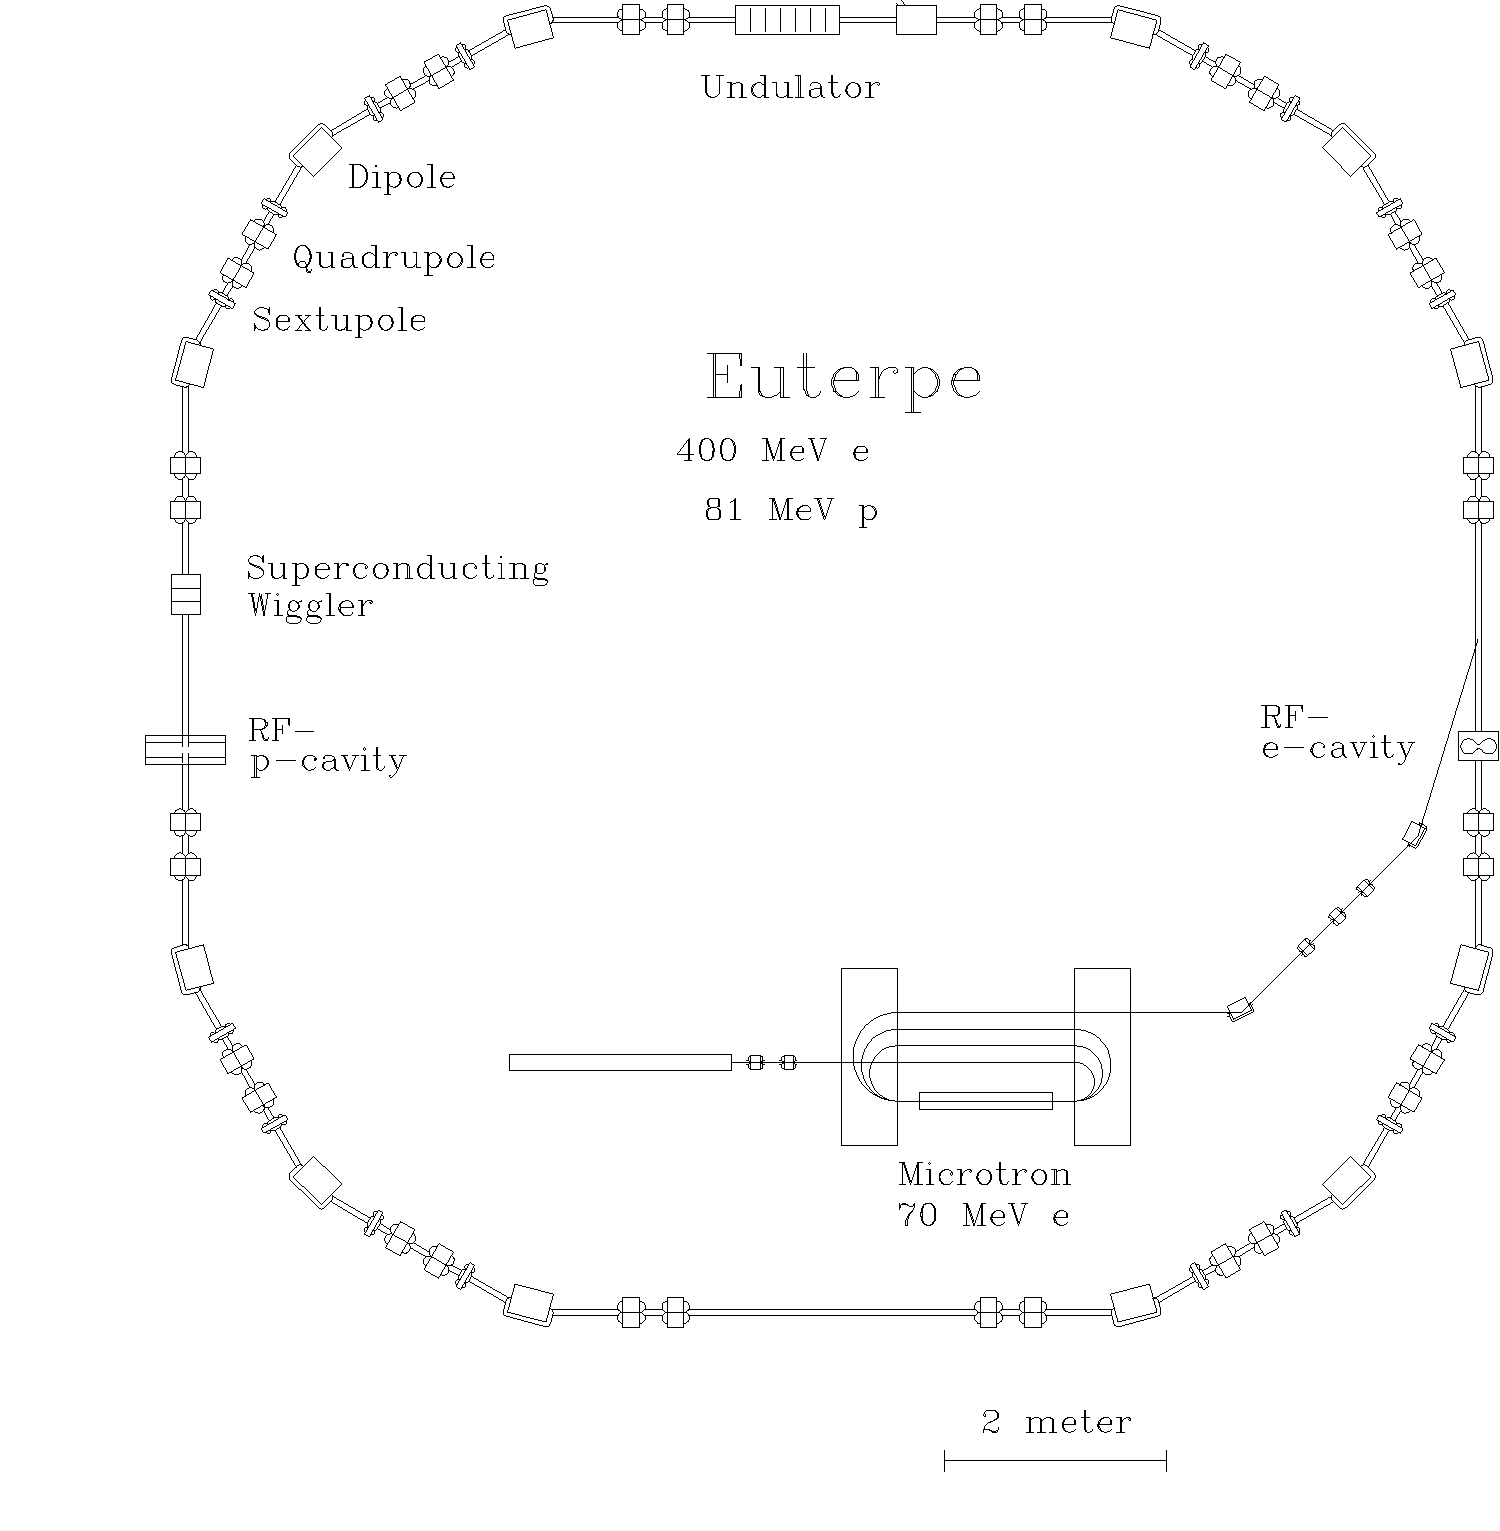
\includegraphics[width=10cm]{euterpe.pdf}~~~~~~}
\vfill
\hrule
\newpage
\thispagestyle{empty}
\copyright~1995, 2022~~J.C.A. Wevers\hfill Version: November 22, 2022
\npar
\hrule
\par
\bigskip
Dear reader,
\npar
This document contains a 108 page \LaTeX\ file which contains a lot equations
in physics. It is written at advanced undergraduate/postgraduate level. It is
intended to be a short reference for anyone who works with physics and often
needs to look up equations.
\npar
This, and a Dutch version of this file, can be obtained from the author,
Johan Wevers\linebreak ({\tt johanw@xs4all.nl}).
\npar
It can also be obtained on the WWW. See
{\tt http://www.xs4all.nl/\~{}johanw/index.html}, where also Postscript
and PDF versions are available.
\npar
If you find any errors or have any comments, please let me know. I am always
open for suggestions and possible corrections to the physics formulary.
\npar
The Physics Formulary is made with MiK\TeX.
\npar
If you prefer the notation in which
vectors are typefaced in boldface, uncomment the redefinition of the
{\tt $\backslash$vec} command in the \TeX\ file and recompile the file.
\npar
This work is licenced under the Creative Commons Attribution 3.0 Netherlands License.
To view a copy of this licence, visit {\tt http://creativecommons.org/licenses/by/3.0/nl/} or send
a letter to Creative Commons, 171 Second Street, Suite 300, San Francisco, California 94105, USA.
\npar
Johan Wevers
\vfill
\hrule
\newpage

\pagenumbering{Roman}
\addcontentsline{toc}{chapter}{Contents}
\typeout{Contents}
\tableofcontents
\newpage

\pagenumbering{arabic}

\chapter*{\center Physical Constants}
\typeout{Physical Constants}
\addcontentsline{toc}{chapter}{Physical Constants}
\begin{center}
\begin{tabular}{||l|lll||}
\hline
{\bf Name}&{\bf Symbol}&{\bf Value}&{\bf Unit}\\
\hline
\hline
Number $\pi$                 &$\pi$&3.14159265358979323846...&\\
Number e                     &e    &2.71828182845904523536...&\\
Euler's constant &\multicolumn{3}{|l||}{$\gamma=\lim\limits_{n\rightarrow\infty}\left(\sum\limits_{k=1}^n 1/k-\ln(n)\right)=0.5772156649...$}\\
\hline
Elementary charge            &$e$&$1.602176634\cdot10^{-19}$&C\rule{0pt}{13pt}\\
Gravitational constant       &$G,\kappa$&$6.67430(15)\cdot10^{-11}$&m$^3$kg$^{-1}$s$^{-2}$\\
Fine-structure constant      &$\alpha=e^2/2hc\varepsilon_0$&$\approx1/137$&\\
Speed of light in vacuum     &$c$&$2.99792458\cdot10^8$&m/s (def)\\
Permittivity of the vacuum   &$\varepsilon_0$&$8.8541878128(13)\cdot10^{-12}$&F/m\\
Permeability of the vacuum   &$\mu_0$&$4\pi\cdot10^{-7}$&H/m\\
$(4\pi\varepsilon_0)^{-1}$   &&$8.9876\cdot10^9$&Nm$^2$C$^{-2}$\\
\hline
Planck's constant            &$h$&$6.62607015\cdot10^{-34}$&Js\rule{0pt}{13pt}\\
Dirac's constant             &$\hbar=h/2\pi$&$1.054571817\cdot10^{-34}$&Js\\
Bohr magneton                &$\mu_{\rm B}=e\hbar/2m_{\rm e}$&$9.2740100783(28)\cdot10^{-24}$&Am$^2$\\
Bohr radius                  &$a_0$&$0.529177210903(80)$&\AA\\
Rydberg's constant           &$Ry$&13.605693122994(26)&eV\\
Electron Compton wavelength  &$\lambda_{\rm Ce}=h/\me c$&$2.42631023867(73)\cdot10^{-12}$&m\\
Proton Compton wavelength    &$\lambda_{\rm Cp}=h/m_{\rm p}c$&$1.32140985539(40)\cdot10^{-15}$&m\\
Reduced mass of the H-atom   &$\mu_{\rm H}$&$9.1045755\cdot10^{-31}$&kg\\
\hline
Stefan-Boltzmann's constant  &$\sigma$&$5.670374419\cdot10^{-8}$&Wm$^{-2}$K$^{-4}$\rule{0pt}{13pt}\\
Wien's constant              &$k_{\rm W}$&$2.897771955...\cdot10^{-3}$&mK\\
\hline
Molar gasconstant            &$R$&8.31446261815324&J$\cdot$mol$^{-1}\cdot$K$^{-1}$\\
Avogadro's constant          &$N_{\rm A}$&$6.02214076\cdot10^{23}$&mol$^{-1}$\\
Boltzmann's constant         &$k=R/N_{\rm A}$&$1.380649\cdot10^{-23}$&J/K\\
\hline
Electron mass                &$m_{\rm e}$&$9.1093837015(28)\cdot10^{-31}$&kg\rule{0pt}{13pt}\\
Proton mass                  &$m_{\rm p}$&$1.67262192369(51)\cdot10^{-27}$&kg\\
Neutron mass                 &$m_{\rm n}$&$1.67492749804(95)\cdot10^{-27}$&kg\\
Elementary mass unit         &$m_{\rm u}=\frac{1}{12}m(^{12}_{~6}$C)&$1.66053906660(50)\cdot10^{-27}$&kg\\
Nuclear magneton             &$\mu_{\rm N}$&$5.050783699(31)\cdot10^{-27}$&J/T\\
\hline
Diameter of the Sun          &$D_\odot$&$1392\cdot10^6$&m\rule{0pt}{13pt}\\
Mass of the Sun              &$M_\odot$&$1.989\cdot10^{30}$&kg\\
Rotational period of the Sun &$T_\odot$&25.38&days\\
Radius of Earth              &$R_{\rm A}$&$6.378\cdot10^6$&m\\
Mass of Earth                &$M_{\rm A}$&$5.976\cdot10^{24}$&kg\\
Rotational period of Earth   &$T_{\rm A}$&23.96&hours\\
Earth orbital period         &Tropical year&365.24219879&days\\
Astronomical unit            &AU&$1.4959787066\cdot10^{11}$&m\\
Light year                   &lj&$9.4605\cdot10^{15}$&m\\
Parsec                       &pc&$3.0857\cdot10^{16}$&m\\
Hubble constant              &$H$&$\approx(75\pm25)$&km$\cdot$s$^{-1}\cdot$Mpc$^{-1}$\\
\hline
\end{tabular}
\end{center}

\renewcommand{\chaptermark}[1]{\markboth{#1}{#1}}
\lhead[\fancyplain{}{\thepage}]{\fancyplain{}{\cmu Chapter \thechapter: \leftmark}}
\rhead[\fancyplain{}{\cmu Physics Formulary by ir. J.C.A. Wevers}]{\fancyplain{}{\thepage}}

\chapter{Mechanics}
\typeout{Mechanics}
\section{Point-kinetics in a fixed coordinate system}
\subsection{Definitions}
The position $\rr$, the velocity $\vv$ and the acceleration $\aaa$ are defined
by:
$\rr=(x,y,z)$, $\vv=(\dot{x},\dot{y},\dot{z})$, $\aaa=(\ddot{x},\ddot{y},\ddot{z})$.
The following holds:
\[
s(t)=s_0+\int|\vv(t)|dt~;~~~\rr(t)=\rr_0+\int\vv(t)dt~;~~~\vv(t)=\vv_0+\int\aaa(t)dt
\]
When the acceleration is constant this gives: $v(t)=v_0+at$ and
$s(t)=s_0+v_0t+\half at^2$.

For the unit vectors in a direction $\perp$ to the orbit $\e{t}$ and parallel
to it $\e{n}$ holds:
\[
\e{t}=\frac{\vv}{|\vv|}=\frac{d\rr}{ds}~~~\dot{\e{t}}=
\frac{v}{\rho}\e{n}~;~~~\e{n}=\frac{\dot{\e{t}}}{|\dot{\e{t}}|}
\]
For the {\it curvature} $k$ and the {\it radius of curvature} $\rho$ holds:
\[
\vec{k}=\frac{d\e{t}}{ds}=\frac{d^2\rr}{ds^2}=\left|\frac{d\varphi}{ds}\right|
~;~~~\rho=\frac{1}{|k|}
\]
\subsection{Polar coordinates}
Polar coordinates are defined by: $x=r\cos(\theta)$, $y=r\sin(\theta)$.
So, for the unit coordinate vectors holds: $\dot{\ee{r}}=\dot{\theta}\ee{\theta}$,
$\dot{\ee{\theta}}=-\dot{\theta}\ee{r}$
\npar
The velocity and the acceleration are derived from: $\rr=r\ee{r}$,
$\vv=\dot{r}\ee{r}+r\dot{\theta}\ee{\theta}$,
$\aaa=(\ddot{r}-r\dot{\theta}^2)\ee{r}+(2\dot{r}\dot{\theta}+r\ddot{\theta})\ee{\theta}$.

\section{Relative motion}
For the motion of a point D w.r.t. a point Q holds:
$\displaystyle\rr_{\rm D}=\rr_{\rm Q}+\frac{\vec{\omega}\times\vv_{\rm Q}}{\omega^2}$
with $\vec{\rm QD}=\rr_{\rm D}-\rr_{\rm Q}$ and $\omega=\dot{\theta}$.
\npar
Further holds: $\alpha=\ddot{\theta}$. $'$ means that the quantity is defined
in a moving system of coordinates. In a moving system holds:\\
$\vv=\vv_{\rm Q}+\vv\,'+\vec{\omega}\times\rr\,'$ and
$\aaa=\aaa_{\rm Q}+\aaa\,'+\vec{\alpha}\times\rr\,'+2\vec{\omega}\times\vv\,'+\vec{\omega}\times(\vec{\omega}\times\rr\,')$\\
with $\vec{\omega}\times(\vec{\omega}\times\rr\,')=-\omega^2\rr\,'_n$

\section{Point-dynamics in a fixed coordinate system}
\subsection{Force, (angular)momentum and energy}
Newton's 2nd law connects the force on an object and the resulting
acceleration of the object where the {\it momentum} is given by
$\vec{p}=m\vv$:
\[
\vec{F}(\rr,\vv,t)=\frac{d\vec{p}}{dt}=\frac{d(m\vv\,)}{dt}=m\frac{d\vv}{dt}+
\vv\,\frac{dm}{dt}\mathop{=}\limits^{m={\rm const}}m\aaa
\]
Newton's 3rd law is given by: $\vec{F}_{\rm action}=-\vec{F}_{\rm reaction}$.
\npar
For the power $P$ holds: $P=\dot{W}=\vec{F}\cdot\vv$. For the total
energy $W$, the kinetic energy $T$ and the potential energy $U$ holds:
$W=T+U~;~~~\dot{T}=-\dot{U}$ with $T=\half mv^2$.
\npar
The {\it kick} $\vec{S}$ is given by:
$\displaystyle\vec{S}=\Delta\vec{p}=\int\vec{F}dt$
\npar
The work $A$, delivered by a force, is
$\displaystyle A=\int\limits_1^2\vec{F}\cdot d\vec{s}=\int\limits_1^2F\cos(\alpha)ds$
\npar
The torque $\vec{\tau}$ is related to the angular momentum
$\vec{L}$:~~$\vec{\tau}=\dot{\vec{L}}=\rr\times\vec{F}$; and\\
$\vec{L}=\rr\times\vec{p}=m\vv\times\rr$, $|\vec{L}|=mr^2\omega$. The
following equation is valid:
\[
\tau=-\Q{U}{\theta}
\]
Hence, the conditions for a mechanical equilibrium are: $\sum\vec{F}_i=0$ and
$\sum\vec{\tau}_i=0$.
\npar
The {\it force of friction} is usually proportional to the force
perpendicular to the surface, except when the motion starts, when a
threshold has to be overcome: $F_{\rm fric}=f\cdot F_{\rm norm}\cdot\e{t}$.

\subsection{Conservative force fields}
A conservative force can be written as the gradient of a potential:
$\vec{F}_{\rm cons}=-\vec{\nabla}U$. From this follows that
$\nabla\times\vec{F}=\vec{0}$. For such a force field also holds:
\[
\oint\vec{F}\cdot d\vec{s}=0~\Rightarrow~U=U_0-\int\limits_{r_0}^{r_1}\vec{F}\cdot d\vec{s}
\]
So the work delivered by a conservative force field depends not on the
trajectory covered but only on the starting and ending points of the motion.

\subsection{Gravitation}
The Newtonian law of gravitation is (in GRT one also uses $\kappa$ instead of $G$):
\[
\vec{F}_{\rm g}=-G\frac{m_1 m_2}{r^2}\ee{r}
\]
The gravitational potential is then given by $V=-Gm/r$. From Gauss law it then
follows: $\nabla^2 V=4\pi G\varrho$.

\subsection{Orbital equations}
If $V=V(r)$ one can derive from the equations of Lagrange for $\phi$ the
conservation of angular momentum:
\[
\Q{\LL}{\phi}=\Q{V}{\phi}=0\Rightarrow\frac{d}{dt}(mr^2\phi)=0\Rightarrow L_z=mr^2\phi=\mbox{constant}
\]
For the radial position as a function of time can be found that:
\[
\left(\frac{dr}{dt}\right)^2=\frac{2(W-V)}{m}-\frac{L^2}{m^2r^2}
\]
The angular equation is then:
\[
\phi-\phi_0=\int\limits_0^r\left[\frac{mr^2}{L}\sqrt{\frac{2(W-V)}{m}-\frac{L^2}{m^2r^2}}~\right]^{-1}dr
\stackrel{r^{-2}{\rm field}}{=}
\arccos\left(1+\frac{\frac{1}{r}-\frac{1}{r_0}}{\frac{1}{r_0}+km/L_z^2}\right)
\]
If $F=F(r)$: $L=$constant, if $F$ is conservative: $W=$constant, if
$\vec{F}\perp\vv$ then $\Delta T=0$ and $U=0$.

\subsubsection{Kepler's orbital equations}
In a force field $F=kr^{-2}$, the orbits are conic sections with the origin of
the force in one of the foci (Kepler's 1st law). The equation of the orbit is:
\[
r(\theta)=\frac{\ell}{1+\varepsilon\cos(\theta-\theta_0)}~,~~\mbox{or:~~}
x^2+y^2=(\ell-\varepsilon x)^2
\]
with
\[
\ell=\frac{L^2}{G\mu^2M_{\rm tot}}~;~~~\varepsilon^2=1+\frac{2WL^2}{G^2\mu^3M^2_{\rm tot}}=1-\frac{\ell}{a}
~;~~~a=\frac{\ell}{1-\varepsilon^2}=\frac{k}{2W}
\]
$a$ is half the length of the long axis of the elliptical orbit in case the
orbit is closed. Half the length of the short axis is $b=\sqrt{a\ell}$.
$\varepsilon$ is the {\it excentricity} of the orbit. Orbits with an equal
$\varepsilon$ are of equal shape. Now, 5 types of orbits are possible:
\begin{enumerate}
\item $k<0$ and $\varepsilon=0$: a circle.
\item $k<0$ and $0<\varepsilon<1$: an ellipse.
\item $k<0$ and $\varepsilon=1$: a parabole.
\item $k<0$ and $\varepsilon>1$: a hyperbole, curved towards the centre of force.
\item $k>0$ and $\varepsilon>1$: a hyperbole, curved away from the centre of force.
\end{enumerate}
Other combinations are not possible: the total energy in a repulsive
force field is always positive so $\varepsilon>1$.
\npar
If the surface between the orbit covered between $t_1$ and $t_2$ and the
focus C around which the planet moves is $A(t_1,t_2)$, Kepler's 2nd law is
\[
A(t_1,t_2)=\frac{L_{\rm C}}{2m}(t_2-t_1)
\]
Kepler's 3rd law is, with $T$ the period and $M_{\rm tot}$ the total mass of
the system:
\[
\frac{T^2}{a^3}=\frac{4\pi^2}{GM_{\rm tot}}
\]
\subsection{The virial theorem}
The virial theorem for one particle is:
\[
\av{m\vv\cdot\rr}=0\Rightarrow\av{T}=-\half\av{\vec{F}\cdot\rr}=\half\av{r\frac{dU}{dr}}=
\half n\av{U}\mbox{ if } U=-\frac{k}{r^n}
\]
The virial theorem for a collection of particles is:
\[
\av{T}=-\half\av{\sum\limits_{\rm particles}\vec{F}_i\cdot\rr_i+
\sum\limits_{\rm pairs}\vec{F}_{ij}\cdot\rr_{ij}}
\]
These propositions can also be written as: $2E_{\rm kin}+E_{\rm pot}=0$.

\section{Point dynamics in a moving coordinate system}
\subsection{Apparent forces}
The total force in a moving coordinate system can be found by subtracting
the apparent forces from the forces working in the reference frame:
$\vec{F}\,'=\vec{F}-\vec{F}_{\rm app}$. The different apparent forces are
given by:
\begin{enumerate}
\item Transformation of the origin: $F_{\rm or}=-m\aaa_a$
\item Rotation: $\vec{F}_{\alpha}=-m\vec{\alpha}\times\rr\,'$
\item Coriolis force: $F_{\rm cor}=-2m\vec{\omega}\times\vv$
\item Centrifugal force: $\vec{F}_{\rm cf}=m\omega^2\rr_n\,'=-\vec{F}_{\rm cp}$
      ;~~$\displaystyle\vec{F}_{\rm cp}=-\frac{mv^2}{r}\ee{r}$
\end{enumerate}

\subsection{Tensor notation}
Transformation of the Newtonian equations of motion to $x^\alpha=x^\alpha(x)$
gives:
\[
\frac{dx^\alpha}{dt}=\Q{x^\alpha}{\bar{x}^\beta}\frac{d\bar{x}^\beta}{dt};
\]
The chain rule gives:
\[
\frac{d}{dt}\frac{dx^\alpha}{dt}=\frac{d^2x^\alpha}{dt^2}=\frac{d}{dt}
\left(\Q{x^\alpha}{\bar{x}^\beta}\frac{d\bar{x}^\beta}{dt}\right)=
\Q{x^\alpha}{\bar{x}^\beta}\frac{d^2\bar{x}^\beta}{dt^2}+
\frac{d\bar{x}^\beta}{dt}\frac{d}{dt}\left(\Q{x^\alpha}{\bar{x}^\beta}\right)
\]
so:
\[
\frac{d}{dt}\Q{x^\alpha}{\bar{x}^\beta}=\Q{}{\bar{x}^\gamma}\Q{x^\alpha}{\bar{x}^\beta}\frac{d\bar{x}^\gamma}{dt}=
\frac{\partial^2x^\alpha}{\partial\bar{x}^\beta\partial\bar{x}^\gamma}\frac{d\bar{x}^\gamma}{dt}
\]
This leads to:
\[
\frac{d^2x^\alpha}{dt^2}=\Q{x^\alpha}{\bar{x}^\beta}\frac{d^2\bar{x}^\beta}{dt^2}+
\frac{\partial^2x^\alpha}{\partial\bar{x}^\beta\partial\bar{x}^\gamma}\frac{d\bar{x}^\gamma}{dt}
\left(\frac{d\bar{x}^\beta}{dt}\right)
\]
Hence the Newtonian equation of motion
\[
m\frac{d^2x^\alpha}{dt^2}=F^\alpha
\]
will be transformed into:
\[
m\left\{\frac{d^2x^\alpha}{dt^2}+\Gamma_{\beta\gamma}^\alpha
\frac{dx^\beta}{dt}\frac{dx^\gamma}{dt}\right\}=F^\alpha
\]
The apparent forces are taken from he origin to the effect side in
the way $\displaystyle\Gamma_{\beta\gamma}^\alpha\frac{dx^\beta}{dt}\frac{dx^\gamma}{dt}$.

\section{Dynamics of masspoint collections}
\subsection{The centre of mass}
The velocity w.r.t. the centre of mass $\vec{R}$ is given by $\vv-\dot{\vec{R}}$.
The coordinates of the centre of mass are given by:
\[
\rr_{\rm m}=\frac{\sum m_i\rr_i}{\sum m_i}
\]
In a 2-particle system, the coordinates of the centre of mass are given by:
\[
\vec{R}=\frac{m_1\rr_1+m_2\rr_2}{m_1+m_2}
\]
With $\rr=\rr_1-\rr_2$, the kinetic energy becomes:
$T=\half M_{\rm tot}\dot{R}^2+\half\mu\dot{r}^2$, with the {\it reduced mass}
$\mu$ given by: $\displaystyle\frac{1}{\mu}=\frac{1}{m_1}+\frac{1}{m_2}$\\
The motion within and outside the centre of mass can be separated:
\[
\dot{\vec{L}}_{\rm outside}=\vec{\tau}_{\rm outside}~;~~~
\dot{\vec{L}}_{\rm inside}=\vec{\tau}_{\rm inside}
\]
\[
\vec{p}=m\vv_{\rm m}~;~~~\vec{F}_{\rm ext}=m\aaa_{\rm m}~;~~~\vec{F}_{12}=\mu\vec{u}
\]
\subsection{Collisions}
With collisions, where B are the coordinates of the collision and C an
arbitrary other position, holds: $\vec{p}=m\vv_{\rm m}$ is constant, and
$T=\half m\vv_{\rm m}^{\,2}$ is constant. The changes in the
{\it relative velocities} can be derived from:
$\vec{S}=\Delta\vec{p}=\mu(\vv_{\rm aft}-\vv_{\rm before})$. Further holds
$\Delta\vec{L}_{\rm C}=\vec{\rm CB}\times\vec{S}$,
$\vec{p}~\parallel~\vec{S}=$constant and $\vec{L}$ w.r.t. B is constant.

\section{Dynamics of rigid bodies}
\subsection{Moment of Inertia}
The angular momentum in a moving coordinate system is given by:
\[
\vec{L}'=I\vec{\omega}+\vec{L}_n'
\]
where $I$ is the {\it moment of inertia} with respect to a central axis,
which is given by:
\[
I=\sum\limits_i m_i\rr_i~^2~;~~~T'=W_{\rm rot}=\half\omega I_{ij}\vec{e}_i\vec{e}_j=\half I\omega^2
\]
or, in the continuous case:
\[
I=\frac{m}{V}\int{r'}^2_ndV=\int{r'}^2_ndm
\]
Further holds:
\[
L_i=I^{ij}\omega_j~;~~~I_{ii}=I_i~;~~~I_{ij}=I_{ji}=-\sum\limits_km_kx_i'x_j'
\]
Steiner's theorem is: $I_{\rm w.r.t. D}=I_{\rm w.r.t. C}+m(DM)^2$ if axis
C $\parallel$ axis D.

\begin{center}
\begin{tabular}{||l|l||l|l||}
\hline
{\bf Object}&$I$&{\bf Object}&$I$\\
\hline
\hline
\rule{0pt}{15pt}Cavern cylinder                   &$I=mR^2$                 &Massive cylinder      &$I=\half mR^2$\\
\rule{0pt}{15pt}Disc, axis in plane disc through m&$I=\kwart mR^2$          &Halter                &$I=\half\mu R^2$\\
\rule{0pt}{15pt}Cavern sphere                     &$I=\frac{2}{3}mR^2$      &Massive sphere        &$I=\frac{2}{5}mR^2$\\
\rule{0pt}{15pt}Bar, axis $\perp$ through c.o.m.  &$I=\frac{1}{12}ml^2$     &Bar, axis $\perp$ through end &$I=\frac{1}{3}ml^2$\\
\rule[-5pt]{0pt}{20pt}Rectangle, axis $\perp$ plane thr. c.o.m.&$I=\frac{1}{12}m(a^2+b^2)$&Rectangle, axis $\parallel b$ thr. m &$I=ma^2$\\
\hline
\end{tabular}
\end{center}

\subsection{Principal axes}
Each rigid body has (at least) 3 principal axes which stand $\perp$ to each
other. For a principal axis holds:
\[
\Q{I}{\omega_x}=\Q{I}{\omega_y}=\Q{I}{\omega_z}=0~~\mbox{so}~~L'_n=0
\]
The following holds: $\dot{\omega}_k=-a_{ijk}\omega_i\omega_j$ with
$\displaystyle a_{ijk}=\frac{I_i-I_j}{I_k}$ if $I_1\leq I_2\leq I_3$.

\subsection{Time dependence}
For torque of force $\vec{\tau}$ holds:
\[
\vec{\tau}\,'=I\ddot{\theta}~;~~~\frac{d''\vec{L}'}{dt}=\vec{\tau}\,'-\vec{\omega}\times\vec{L}'
\]
The {\it torque} $\vec{T}$ is defined by: $\vec{T}=\vec{F}\times\vec{d}$.

\section{Variational Calculus, Hamilton and Lagrange mechanics}
\subsection{Variational Calculus}
Starting with:
\[
\delta\int\limits_a^b\LL(q,\dot{q},t)dt=0\mbox{~~with~~}\delta(a)=\delta(b)=0\mbox{~~and~~}
\delta\left(\frac{du}{dx}\right)=\frac{d}{dx}(\delta u)
\]
the equations of Lagrange can be derived:
\[
\frac{d}{dt}\Q{\LL}{\dot{q}_i}=\Q{\LL}{q_i}
\]
When there are additional conditions applying to the variational problem
$\delta J(u)=0$ of the type $K(u)=$constant, the new problem becomes:
$\delta J(u)-\lambda\delta K(u)=0$.

\subsection{Hamilton mechanics}
The {\it Lagrangian} is given by: $\LL=\sum T(\dot{q}_i)-V(q_i)$.
The {\it Hamiltonian} is given by: $H=\sum\dot{q}_ip_i-\LL$. In 2
dimensions holds: $\LL=T-U=\half m(\dot{r}^2+r^2\dot{\phi}^2)-U(r,\phi)$.
\npar
If the used coordinates are {\it canonical} the Hamilton equations are
the equations of motion for the system:
\[
\frac{dq_i}{dt}=\Q{H}{p_i}~;~~~\frac{dp_i}{dt}=-\Q{H}{q_i}
\]
Coordinates are canonical if the following holds:
$\{q_i,q_j\}=0,~\{p_i,p_j\}=0,~\{q_i,p_j\}=\delta_{ij}$ where $\{,\}$ is the
{\it Poisson bracket}:
\[
\{A,B\}=\sum\limits_i\left[\Q{A}{q_i}\Q{B}{p_i}-\Q{A}{p_i}\Q{B}{q_i}\right]
\]
The Hamiltonian of a Harmonic oscillator is given by
$H(x,p)=p^2/2m+\half m\omega^2 x^2$. With new coordinates $(\theta,I)$,
obtained by the canonical transformation $x=\sqrt{2I/m\omega}\cos(\theta)$
and $p=-\sqrt{2Im\omega}\sin(\theta)$, with inverse $\theta=\arctan(-p/m\omega x)$
and $I=p^2/2m\omega+\half m\omega x^2$ it follows: $H(\theta,I)=\omega I$.
\npar
The Hamiltonian of a charged particle with charge $q$ in an external
electromagnetic field is given by:
\[
H=\frac{1}{2m}\left(\vec{p}-q\vvec{A}\right)^2+qV
\]
This Hamiltonian can be derived from the Hamiltonian of a free particle
$H=p^2/2m$ with the transformations $\vec{p}\rightarrow\vec{p}-q\vec{A}$ and
$H\rightarrow H-qV$. This is elegant from a relativistic point of view: this
is equivalent to the transformation of the momentum 4-vector
$p^\alpha\rightarrow p^\alpha-qA^\alpha$. A gauge transformation on the
potentials $A^\alpha$ corresponds with a canonical transformation, which make
the Hamilton equations the equations of motion for the system.

\subsection{Motion around an equilibrium, linearization}
For natural systems around equilibrium the following equations are valid:
\[
\left(\Q{V}{q_i}\right)_0=0~;~~~V(q)=V(0)+V_{ik}q_iq_k\mbox{~~with~~}
V_{ik}=\left(\frac{\partial^2V}{\partial q_i\partial q_k}\right)_0
\]
With $T=\half(M_{ik}\dot{q}_i\dot{q}_k)$ one receives the set of equations
$M\ddot{q}+Vq=0$. If $q_i(t)=a_i\exp(i\omega t)$ is substituted, this set
of equations has solutions if ${\rm det}(V-\omega^2 M)=0$. This leads to
the eigenfrequencies of the problem:
$\displaystyle\omega^2_k=\frac{a_k^{\rm T}Va_k}{a_k^{\rm T}Ma_k}$.
If the equilibrium is stable holds: $\forall k$ that $\omega^2_k>0$. The
general solution is a superposition if eigenvibrations.

\subsection{Phase space, Liouville's equation}
In phase space holds:
\[
\nabla=\left(\sum_i\Q{}{q_i},\sum_i\Q{}{p_i}\right)\mbox{~~so~~}
\nabla\cdot\vv=\sum_i\left(\Q{}{q_i}\Q{H}{p_i}-\Q{}{p_i}\Q{H}{q_i}\right)
\]
If the equation of continuity, $\partial_t\varrho+\nabla\cdot(\varrho\vv\,)=0$
holds, this can be written as:
\[
\{\varrho,H\}+\Q{\varrho}{t}=0
\]
For an arbitrary quantity $A$ holds:
\[
\frac{dA}{dt}=\{A,H\}+\Q{A}{t}
\]
Liouville's theorem can than be written as:
\[
\frac{d\varrho}{dt}=0~;~~~\mbox{or:~}\int pdq=\mbox{constant}
\]
\subsection{Generating functions}
Starting with the coordinate transformation:
\[
\left\{\begin{array}{l}
Q_i=Q_i(q_i,p_i,t)\\
P_i=P_i(q_i,p_i,t)
\end{array}\right.
\]
one can derive the following Hamilton equations with the new Hamiltonian $K$:
\[
\frac{dQ_i}{dt}=\Q{K}{P_i}~;~~~\frac{dP_i}{dt}=-\Q{K}{Q_i}
\]
Now, a distinction between 4 cases can be made:
\begin{enumerate}
\item If $\displaystyle p_i\dot{q}_i-H=P_iQ_i-K(P_i,Q_i,t)-\frac{dF_1(q_i,Q_i,t)}{dt}$,
the coordinates follow from:
\[
p_i=\Q{F_1}{q_i}~;~~~P_i=-\Q{F_1}{Q_i}~;~~~K=H+\Q{F_1}{t}
\]
\item If $\displaystyle p_i\dot{q}_i-H=-\dot{P}_iQ_i-K(P_i,Q_i,t)+\frac{dF_2(q_i,P_i,t)}{dt}$,
the coordinates follow from:
\[
p_i=\Q{F_2}{q_i}~;~~~Q_i=\Q{F_2}{P_i}~;~~~K=H+\Q{F_2}{t}
\]
\item If $\displaystyle-\dot{p}_iq_i-H=P_i\dot{Q}_i-K(P_i,Q_i,t)+\frac{dF_3(p_i,Q_i,t)}{dt}$,
the coordinates follow from:
\[
q_i=-\Q{F_3}{p_i}~;~~~P_i=-\Q{F_3}{Q_i}~;~~~K=H+\Q{F_3}{t}
\]
\item If $\displaystyle-\dot{p}_iq_i-H=-P_iQ_i-K(P_i,Q_i,t)+\frac{dF_4(p_i,P_i,t)}{dt}$,
the coordinates follow from:
\[
q_i=-\Q{F_4}{p_i}~;~~~Q_i=\Q{F_4}{P_i}~;~~~K=H+\Q{F_4}{t}
\]
\end{enumerate}
The functions $F_1$, $F_2$, $F_3$ and $F_4$ are called {\it generating functions}.

\chapter{Electricity \& Magnetism}
\typeout{Electricity & Magnetism}
\section{The Maxwell equations}
The classical electromagnetic field can be described by the
{\it Maxwell equations}. Those can be written both as differential and
integral equations:
\[
\begin{array}{ll}
\displaystyle\oiint(\vec{D}\cdot\vec{n}\,)d^2A=Q_{\rm free,included}~~~~~~~~~~~~~
 &\displaystyle\nabla\cdot\vec{D}=\rho_{\rm free}\\
\displaystyle\oiint(\vec{B}\cdot\vec{n}\,)d^2A=0
 &\displaystyle\nabla\cdot\vec{B}=0\\
\displaystyle\oint\vec{E}\cdot d\vec{s}=-\frac{d\Phi}{dt}
 &\displaystyle\nabla\times\vec{E}=-\Q{\vec{B}}{t}\\
\displaystyle\oint\vec{H}\cdot d\vec{s}=I_{\rm free,included}+\frac{d\Psi}{dt}
 &\displaystyle\nabla\times\vec{H}=\vec{J}_{\rm free}+\Q{\vec{D}}{t}
\end{array}
\]
For the fluxes holds: $\displaystyle \Psi=\iint(\vec{D}\cdot\vec{n}\,)d^2A$,
$\displaystyle\Phi=\iint(\vec{B}\cdot\vec{n}\,)d^2A$.
\npar
The electric displacement $\vec{D}$, polarization $\vec{P}$ and
electric field strength $\vec{E}$ depend on each other according to:
\npar
$\vec{D}=\varepsilon_0\vec{E}+\vec{P}=\varepsilon_0\varepsilon_{\rm r}\vec{E}$,~~
$\vec{P}=\sum\vec{p}_0/{\rm Vol}$, $\varepsilon_{\rm r}=1+\chi_{\rm e}$, with
$\displaystyle\chi_{\rm e}=\frac{np_0^2}{3\varepsilon_0kT}$
\npar
The magnetic field strength $\vec{H}$, the magnetization $\vec{M}$ and the
magnetic flux density $\vec{B}$ depend on each other according to:
\npar
$\vec{B}=\mu_0(\vec{H}+\vec{M})=\mu_0\mu_{\rm r}\vec{H}$,~~
$\vec{M}=\sum\vec{m}/{\rm Vol}$, $\mu_{\rm r}=1+\chi_{\rm m}$, with
$\displaystyle\chi_{\rm m}=\frac{\mu_0nm_0^2}{3kT}$

\section{Force and potential}
The force and the electric field between 2 point charges are given by:
\[
\vec{F}_{12}=\frac{Q_1Q_2}{4\pi\varepsilon_0\varepsilon_{\rm r}r^2}\ee{r}
~;~~~\vec{E}=\frac{\vec{F}}{Q}
\]
The Lorentzforce is the force which is felt by a charged particle that moves
through a magnetic field. The origin of this force is a relativistic
transformation of the Coulomb force:
$\vec{F}_{\rm L}=Q(\vv\times\vvec{B})=l(\vec{I}\times\vvec{B})$.
\npar
The magnetic field in point $P$ which results from an electric current is
given by the {\it law of Biot-Savart}, also known as the law of Laplace.
In here, $d\vec{l}\parallel\vec{I}$ and $\rr$ points from $d\vec{l}$
to $P$:
\[
d\vec{B}_P=\frac{\mu_0I}{4\pi r^2}d\vec{l}\times\ee{r}
\]
If the current is time-dependent one has to take {\it retardation} into
account: the substitution $I(t)\rightarrow I(t-r/c)$ has to be applied.
\npar
The potentials are given by:
$\displaystyle V_{12}=-\int\limits_1^2\vec{E}\cdot d\vec{s}$ and
$\vec{A}=\half\vec{B}\times\rr$.
\npar
Here, the freedom remains to apply a {\it gauge transformation}. The fields
can be derived from the potentials as follows:
\[
\vec{E}=-\nabla V-\Q{\vec{A}}{t}~,~~~\vec{B}=\nabla\times\vec{A}
\]
Further holds the relation: $c^2\vec{B}=\vv\times\vec{E}$.

\section{Gauge transformations}
The potentials of the electromagnetic fields transform as follows when a
gauge transformation is applied:
\[
\left\{\begin{array}{l}
\vec{A}'=\vec{A}-\nabla f\\
\displaystyle V'=V+\Q{f}{t}
\end{array}\right.
\]
so the fields $\vec{E}$ and $\vec{B}$ do not change. This results in a
canonical transformation of the Hamiltonian. Further, the freedom remains to
apply a limiting condition. Two common choices are:
\begin{enumerate}
\item Lorentz-gauge: $\displaystyle\nabla\cdot\vec{A}+\frac{1}{c^2}\Q{V}{t}=0$.
      This separates the differential equations for $\vec{A}$ and $V$:
      $\displaystyle\Box V=-\frac{\rho}{\varepsilon_0}$, $\Box\vec{A}=-\mu_0\vec{J}$.
\item Coulomb gauge: $\nabla\cdot\vec{A}=0$. If $\rho=0$ and $\vec{J}=0$ holds
      $V=0$ and follows $\vec{A}$ from $\Box\vec{A}=0$.
\end{enumerate}

\section{Energy of the electromagnetic field}
The energy density of the electromagnetic field is:
\[
\frac{dW}{d{\rm Vol}}=w=\int HdB+\int EdD
\]
The energy density can be expressed in the potentials and currents as follows:
\[
w_{\rm mag}=\half\int\vec{J}\cdot\vec{A}\,d^3x~~,~~w_{\rm el}=\half\int\rho Vd^3x
\]

\section{Electromagnetic waves}
\subsection{Electromagnetic waves in vacuum}
The wave equation $\Box\Psi(\rr,t)=-f(\rr,t)$ has the general solution, with
$c=(\varepsilon_0\mu_0)^{-1/2}$:
\[
\Psi(\rr,t)=\int\frac{f(\rr,t-|\rr-\rr\,'|/c)}{4\pi|\rr-\rr\,'|}d^3r'
\]
If this is written as: $\vec{J}(\rr,t)=\vec{J}(\rr\,)\exp(-i\omega t)$ and
$\vec{A}(\rr,t)=\vec{A}(\rr\,)\exp(-i\omega t)$ with:
\[
\vec{A}(\rr\,)=\frac{\mu}{4\pi}\int\vec{J}(\rr\,')\frac{\exp(ik|\rr-\rr\,'|)}{|\rr-\rr\,'|}d^3\rr\,'~~,~~~
V(\rr\,)=\frac{1}{4\pi\varepsilon}\int\rho(\rr\,')\frac{\exp(ik|\rr-\rr\,'|)}{|\rr-\rr\,'|}d^3\rr\,'
\]
A derivation via multipole expansion will show that for the radiated energy
holds, if $d,\lambda\gg r$:
\[
\frac{dP}{d\Omega}=\frac{k^2}{32\pi^2\varepsilon_0c}\left|\int J_\perp(\rr\,'){\rm e}^{i\vec{k}\cdot\rr}d^3r'\right|^2
\]
The energy density of the electromagnetic wave of a vibrating dipole at a
large distance is:
\[
w=\varepsilon_0E^2=\frac{p^2_0\sin^2(\theta)\omega^4}{16\pi^2\varepsilon_0r^2c^4}\sin^2(kr-\omega t)~,~~~
\av{w}_t=\frac{p^2_0\sin^2(\theta)\omega^4}{32\pi^2\varepsilon_0r^2c^4}~,~~
P=\frac{ck^4|\vvec{p}|^2}{12\pi\varepsilon_0}
\]
The radiated energy can be derived from the {\it Poynting vector} $\vec{S}$:
$\vec{S}=\vec{E}\times\vec{H}=cW\vec{e}_v$. The {\it irradiance} is the
time-averaged of the Poynting vector: $I=\langle|\vvec{S}|\rangle_t$. The
radiation pressure $p_{\rm s}$ is given by $p_{\rm s}=(1+R)|\vvec{S}|/c$,
where $R$ is the coefficient of reflection.

\subsection{Electromagnetic waves in matter}
The wave equations in matter, with $c_{\rm mat}=(\varepsilon\mu)^{-1/2}$ the
lightspeed in matter, are:
\[
\left(\nabla^2-\varepsilon\mu\QQ{}{t}-\frac{\mu}{\rho}\Q{}{t}\right)\vec{E}=0~,~~
\left(\nabla^2-\varepsilon\mu\QQ{}{t}-\frac{\mu}{\rho}\Q{}{t}\right)\vec{B}=0
\]
give, after substitution of monochromatic plane waves:
$\vec{E}=E\exp(i(\vec{k}\cdot\rr-\omega t))$ and
$\vec{B}=B\exp(i(\vec{k}\cdot\rr-\omega t))$ the dispersion relation:
\[
k^2=\varepsilon\mu\omega^2+\frac{i\mu\omega}{\rho}
\]
The first term arises from the displacement current, the second from the
conductance current. If $k$ is written in the form $k:=k'+ik''$ it follows
that:
\[
k'=\omega\sqrt{\half\varepsilon\mu}\sqrt{1+\sqrt{1+\frac{1}{(\rho\varepsilon\omega)^2}}}~~~\mbox{and}~~~
k''=\omega\sqrt{\half\varepsilon\mu}\sqrt{-1+\sqrt{1+\frac{1}{(\rho\varepsilon\omega)^2}}}
\]
This results in a damped wave: $\vec{E}=E\exp(-k''\vec{n}\cdot\rr\,)\exp(i(k'\vec{n}\cdot\rr-\omega t))$.
If the material is a good conductor, the wave vanishes after approximately
one wavelength, $\displaystyle k=(1+i)\sqrt{\frac{\mu\omega}{2\rho}}$.

\section{Multipoles}
Because
$\displaystyle
\frac{1}{|\rr-\rr\,'|}=\frac{1}{r}\sum_0^\infty\left(\frac{r'}{r}\right)^lP_l(\cos\theta)$
the potential can be written as:
$\displaystyle V=\frac{Q}{4\pi\varepsilon}\sum_n\frac{k_n}{r^n}$
\npar
For the lowest-order terms this results in:
\begin{itemize}
\item Monopole: $l=0$, $k_0=\int\rho dV$
\item Dipole: $l=1$, $k_1=\int r\cos(\theta)\rho dV$
\item Quadrupole: $l=2$, $k_2=\half\sum\limits_i(3z^2_i-r^2_i)$
\end{itemize}
\begin{enumerate}
\item The electric dipole: dipole moment: $\vec{p}=Ql\e{}$, where $\e{}$
      goes from $\oplus$ to $\ominus$, and
      $\vec{F}=(\vec{p}\cdot\nabla)\vec{E}_{\rm ext}$, and
      $W=-\vec{p}\cdot\vec{E}_{\rm out}$.\\
      Electric field: $\displaystyle \vec{E}\approx\frac{Q}{4\pi\varepsilon r^3}\left(\frac{3\vec{p}\cdot\rr}{r^2}-\vec{p}\right)$.~~
      The torque is: $\vec{\tau}=\vec{p}\times\vec{E}_{\rm out}$
\item The magnetic dipole: dipole moment: if $r\gg\sqrt{A}$: $\vec{\mu}=\vec{I}\times(A\ee{\perp})$,
      $\vec{F}=(\vec{\mu}\cdot\nabla)\vec{B}_{\rm out}$\\
      $\displaystyle|\mu|=\frac{mv^2_\perp}{2B}$, $W=-\vec{\mu}\times\vec{B}_{\rm out}$\\
      Magnetic field: $\displaystyle\vec{B}=\frac{-\mu}{4\pi r^3}\left(\frac{3\mu\cdot\rr}{r^2}-\vec{\mu}\right)$.~~
      The moment is: $\vec{\tau}=\vec{\mu}\times\vec{B}_{\rm out}$
\end{enumerate}

\section{Electric currents}
The continuity equation for charge is:
$\displaystyle\Q{\rho}{t}+\nabla\cdot\vec{J}=0$.
The {\it electric current} is given by:
\[
I=\frac{dQ}{dt}=\iint(\vec{J}\cdot\vvec{n})d^2A
\]
For most conductors holds: $\vec{J}=\vec{E}/\rho$, where $\rho$ is the
{\it resistivity}.
\npar
If the flux enclosed by a conductor changes this results in an
{\it induced voltage} $\displaystyle V_{\rm ind}=-N\frac{d\Phi}{dt}$.
If the current flowing through a conductor changes, this results in a
self-inductance which opposes the original change:
$\displaystyle V_{\rm selfind}=-L\frac{dI}{dt}$.
If a conductor encloses a flux $\Phi$ holds: $\Phi=LI$.
\npar
The magnetic induction within a coil is approximated by:
$\displaystyle B=\frac{\mu NI}{\sqrt{l^2+4R^2}}$ where $l$ is the length, $R$
the radius and $N$ the number of coils. The energy contained within a coil is
given by $W=\half LI^2$ and $L=\mu N^2A/l$.
\npar
The {\it capacity} is defined by: $C=Q/V$. For a capacitor holds:
$C=\varepsilon_0\varepsilon_{\rm r}A/d$ where $d$ is the distance between the
plates and $A$ the surface of one plate. The electric field strength
between the plates is $E=\sigma/\varepsilon_0=Q/\varepsilon_0A$ where $\sigma$
is the surface charge. The accumulated energy is given by $W=\half CV^2$.
The current through a capacity is given by $\displaystyle I=-C\frac{dV}{dt}$.
\npar
For most PTC resistors holds approximately: $R=R_0(1+\alpha T)$,
where $R_0=\rho l/A$. For a NTC holds: $R(T)=C\exp(-B/T)$ where $B$ and $C$
depend only on the material.
\npar
If a current flows through two different, connecting conductors $x$ and $y$,
the contact area will heat up or cool down, depending on the direction of the
current: the {\it Peltier effect}. The generated or removed heat is given by:
$W=\Pi_{xy}It$. This effect can be amplified with semiconductors.
\npar
The {\it thermic voltage} between 2 metals is given by: $V=\gamma(T-T_0)$.
For a Cu-Konstantane connection holds: $\gamma\approx0.2-0.7$ mV/K.
\npar
In an electrical net with only stationary currents, {\it Kirchhoff's}
equations apply: for a knot holds: $\sum I_n=0$, along a closed path holds:
$\sum V_n=\sum I_nR_n=0$.

\section{Depolarizing field}
If a dielectric material is placed in an electric or magnetic field, the
field strength within and outside the material will change because the
material will be polarized or magnetized. If the medium has an ellipsoidal
shape and one of the principal axes is parallel with the external field
$\vec{E}_0$ or $\vec{B}_0$ then the depolarizing is field homogeneous.
\begin{eqnarray*}
\vec{E}_{\rm dep}=\vec{E}_{\rm mat}-\vec{E}_0=-\frac{{\cal N}\vec{P}}{\varepsilon_0}\\
\vec{H}_{\rm dep}=\vec{H}_{\rm mat}-\vec{H}_0=-{\cal N}\vec{M}
\end{eqnarray*}
$\cal N$ is a constant depending only on the shape of the object placed in
the field, with $0\leq{\cal N}\leq1$. For a few limiting cases of an
ellipsoid holds: a thin plane: ${\cal N}=1$, a long, thin bar: ${\cal N}=0$,
a sphere: ${\cal N}=\frac{1}{3}$.

\section{Mixtures of materials}
The average electric displacement in a material which is inhomogenious on a
mesoscopic scale is given by: $\av{D}=\av{\varepsilon E}=\varepsilon^*\av{E}$
where $\displaystyle \varepsilon^*=\varepsilon_1\left(1-\frac{\phi_2(1-x)}{\Phi(\varepsilon^*/\varepsilon_2)}\right)^{-1}$
where $x=\varepsilon_1/\varepsilon_2$. For a sphere holds:
$\Phi=\frac{1}{3}+\frac{2}{3}x$. Further holds:
\[
\left(\sum_i \frac{\phi_i}{\varepsilon_i}\right)^{-1}\leq\varepsilon^*\leq\sum_i \phi_i\varepsilon_i
\]

\chapter{Relativity}
\typeout{Relativity}
\section{Special relativity}
\subsection{The Lorentz transformation}
The Lorentz transformation $(\vvec{x}',t')=(\vvec{x}'(\vec{x},t),t'(\vec{x},t))$
leaves the wave equation invariant if $c$ is invariant:
\[
\QQ{}{x}+\QQ{}{y}+\QQ{}{z}-\frac{1}{c^2}\QQ{}{t}=
\QQ{}{x'}+\QQ{}{y'}+\QQ{}{z'}-\frac{1}{c^2}\QQ{}{t'}
\]
This transformation can also be found when $ds^2=ds'^2$ is demanded. The
general form of the Lorentz transformation is given by:
\[
\vvec{x}'=\vec{x}+\frac{(\gamma-1)(\vec{x}\cdot\vv\,)\vv}{|v|^2}-\gamma\vv t~~,~~
t'=\gamma\left(t-\frac{\vec{x}\cdot\vv}{c^2}\right)
\]
where
\[
\gamma=\frac{1}{\sqrt{1-\frac{\displaystyle v^2}{\displaystyle c^2}}}
\]
The velocity difference $\vv\,'$ between two observers transforms according to:
\[
\vv\,'=\left(\gamma\left(1-\frac{\vv_1\cdot\vv_2}{c^2}\right)\right)^{-1}
\left(\vv_2+(\gamma-1)\frac{\vv_1\cdot\vv_2}{v_1^2}\vv_1-\gamma\vv_1\right)
\]
If the velocity is parallel to the $x$-axis, this becomes $y'=y$, $z'=z$ and:
\begin{eqnarray*}
&&x'=\gamma(x-vt)~,~~~x=\gamma(x'+vt')\\
&&t'=\gamma\left(t-\displaystyle\frac{xv}{c^2}\right)~,~~~t=\gamma\left(t'+\displaystyle\frac{x'v}{c^2}\right)~,~~~
v'=\frac{\displaystyle v_2-v_1}{\displaystyle 1-\frac{v_1v_2}{c^2}}
\end{eqnarray*}
If $\vv=v\vec{e}_x$ holds:
\[
p'_x=\gamma\left(p_x-\frac{\beta W}{c}\right)~,~~~W'=\gamma(W-vp_x)
\]
With $\beta=v/c$ the electric field of a moving charge is given by:
\[
\vec{E}=\frac{Q}{4\pi\varepsilon_0r^2}\frac{(1-\beta^2)\ee{r}}{(1-\beta^2\sin^2(\theta))^{3/2}}
\]
The electromagnetic field transforms according to:
\[
\vec{E}'=\gamma(\vec{E}+\vv\times\vvec{B})~~,~~~
\vec{B}'=\gamma\left(\vec{B}-\frac{\vv\times\vec{E}}{c^2}\right)
\]
Length, mass and time transform according to:
$\Delta t_{\rm r}=\gamma\Delta t_{\rm 0}$, $m_{\rm r}=\gamma m_0$,
$l_{\rm r}=l_0/\gamma$, with $_{\rm 0}$ the quantities in a co-moving
reference frame and $_{\rm r}$ the quantities in a frame moving with velocity
$v$ w.r.t.\ it. The proper time $\tau$ is defined as: $d\tau^2=ds^2/c^2$, so
$\Delta\tau=\Delta t/\gamma$. For energy and momentum holds: $W=m_{\rm
r}c^2=\gamma W_0$, $W^2=m_0^2c^4+p^2c^2$. $p=m_{\rm r}v=\gamma m_0v=Wv/c^2$,
and $pc=W\beta$ where $\beta=v/c$. The {\it force} is {\it defined} by
$\vec{F}=d\vec{p}/dt$.
\npar
4-vectors have the property that their modulus is independent of the
observer: their components {\it can} change after a coordinate transformation
but not their modulus. The difference of two 4-vectors transforms also as a
4-vector. The 4-vector for the velocity is given by
$\displaystyle U^\alpha=\frac{dx^\alpha}{d\tau}$. The relation with the
``common'' velocity $u^i:=dx^i/dt$ is: $U^\alpha=(\gamma u^i,ic\gamma)$.
For particles with nonzero restmass holds: $U^\alpha U_\alpha=-c^2$, for
particles with zero restmass (so with $v=c$) holds: $U^\alpha U_\alpha=0$.
The 4-vector for energy and momentum is given by:
$p^\alpha=m_0U^\alpha=(\gamma p^i,iW/c)$. So:
$p_\alpha p^\alpha=-m_0^2c^2=p^2-W^2/c^2$.

\subsection{Red and blue shift}
There are three causes of red and blue shifts:
\begin{enumerate}
\item Motion: with $\vec{e}_v\cdot\vec{e}_r=\cos(\varphi)$ follows:
      $\displaystyle \frac{f'}{f}=\gamma\left(1-\frac{v\cos(\varphi)}{c}\right)$.\\
      This can give both red- and blueshift, also $\perp$ to the direction of
      motion.
\item Gravitational redshift: $\displaystyle\frac{\Delta f}{f}=\frac{\kappa M}{rc^2}$.
\item Redshift because the universe expands, resulting in e.g.~the
      cosmic background radiation:\\
      $\displaystyle\frac{\lambda_0}{\lambda_1}=\frac{R_0}{R_1}$.
\end{enumerate}

\subsection{The stress-energy tensor and the field tensor}
The stress-energy tensor is given by:
\[
T_{\mu\nu}=(\varrho c^2+p)u_\mu u_\nu+pg_{\mu\nu}+\frac{1}{c^2}
\left(F_{\mu\alpha}F^\alpha_\nu+\kwart g_{\mu\nu}F^{\alpha\beta}F_{\alpha\beta}\right)
\]
The conservation laws can than be written as: $\nabla_\nu T^{\mu\nu}=0$. The
electromagnetic field tensor is given by:
\[
\mbox{\fbox{$\displaystyle F_{\alpha\beta}=\Q{A_\beta}{x^\alpha}-\Q{A_\alpha}{x^\beta}$}}
\]
with $A_\mu:=(\vec{A},iV/c)$ and $J_\mu:=(\vec{J},ic\rho)$. The
Maxwell equations can than be written as:
\[
\partial_\nu F^{\mu\nu}=\mu_0J^\mu~,~~
\partial_\lambda F_{\mu\nu}+\partial_\mu F_{\nu\lambda}+\partial_\nu F_{\lambda\mu}=0
\]
The equations of motion for a charged particle in an EM field become with the
field tensor:
\[
\mbox{\fbox{$\displaystyle\frac{dp_\alpha}{d\tau}=qF_{\alpha\beta}u^\beta$}}
\]

\section{General relativity}
\subsection{Riemannian geometry, the Einstein tensor}
The basic principles of general relativity are:
\begin{enumerate}
\item The geodesic postulate: free falling particles move along geodesics of
      space-time with the proper time $\tau$ or arc length $s$ as parameter.
      For particles with zero rest mass (photons), the use of a free
      parameter is required because for them holds $ds=0$. From
      $\delta\int ds=0$ the equations of motion can be derived:
      \[
      \frac{d^2x^\alpha}{ds^2}+\Gamma_{\beta\gamma}^{\alpha}\frac{dx^\beta}{ds}\frac{dx^\gamma}{ds}=0
      \]
\item The {\it principle of equivalence}: inertial mass $\equiv$ gravitational
      mass $\Rightarrow$ gravitation is equivalent with a curved space-time
      were particles move along geodesics.
\item By a proper choice of the coordinate system it is possible to make the
      metric locally flat in each point $x_i$:
      $g_{\alpha\beta}(x_i)=\eta_{\alpha\beta}:=$diag$(-1,1,1,1)$.
\end{enumerate}
\npar
The {\it Riemann tensor} is defined as:
$R^\mu_{\nu\alpha\beta}T^\nu:=\nabla_\alpha\nabla_\beta T^\mu-\nabla_\beta\nabla_\alpha T^\mu$,
where the covariant derivative is given by
$\nabla_j a^i=\partial_ja^i+\Gamma_{jk}^ia^k$ and
$\nabla_j a_i=\partial_ja_i-\Gamma_{ij}^ka_k$. Here,
\[
\Gamma_{jk}^i=\frac{g^{il}}{2}\left(\frac{\partial g_{lj}}{\partial x^k}+
\frac{\partial g_{lk}}{\partial x^j}-\frac{\partial g_{_jk}}{\partial x^l}\right),
\mbox{ for Euclidean spaces this reduces to: }
\Gamma_{jk}^i=\frac{\partial^2\bar{x}^l}{\partial x^j\partial x^k}\Q{x^i}{\bar{x}^l},
\]
are the {\it Christoffel symbols}. For a second-order tensor holds:
$[\nabla_\alpha,\nabla_\beta]T_\nu^\mu=R_{\sigma\alpha\beta}^\mu T^\sigma_\nu+R^\sigma_{\nu\alpha\beta}T^\mu_\sigma$,
$\nabla_k a^i_j=\partial_ka^i_j-\Gamma_{kj}^la_l^i+\Gamma_{kl}^ia_j^l$,
$\nabla_k a_{ij}=\partial_ka_{ij}-\Gamma_{ki}^la_{lj}-\Gamma_{kj}^la_{jl}$ and
$\nabla_k a^{ij}=\partial_ka^{ij}+\Gamma_{kl}^ia^{lj}+\Gamma_{kl}^ja^{il}$.
The following holds: $R_{\beta\mu\nu}^\alpha=\partial_\mu\Gamma_{\beta\nu}^\alpha-\partial_\nu\Gamma_{\beta\mu}^\alpha+
\Gamma_{\sigma\mu}^\alpha\Gamma_{\beta\nu}^\sigma-\Gamma_{\sigma\nu}^\alpha\Gamma_{\beta\mu}^\sigma$.
\npar
The {\it Ricci tensor} is a contraction of the Riemann tensor:
$R_{\alpha\beta}:=R^\mu_{\alpha\mu\beta}$, which is symmetric:
$R_{\alpha\beta}=R_{\beta\alpha}$. The {\it Bianchi identities} are:
$\nabla_\lambda R_{\alpha\beta\mu\nu}+\nabla_\nu R_{\alpha\beta\lambda\mu}+
\nabla_\mu R_{\alpha\beta\nu\lambda}=0$.
\npar
The {\it Einstein tensor} is given by:
$G^{\alpha\beta}:=R^{\alpha\beta}-\half g^{\alpha\beta}R$, where
$R:=R_\alpha^\alpha$ is the {\it Ricci scalar}, for which holds:
$\nabla_\beta G_{\alpha\beta}=0$. With the variational principle
$\delta\int(\LL(g_{\mu\nu})-Rc^2/16\pi\kappa)\sqrt{|g|}d^4x=0$ for variations
$g_{\mu\nu}\rightarrow g_{\mu\nu}+\delta g_{\mu\nu}$ the
{\it Einstein field equations} can be derived:
\[
\mbox{\fbox{$\displaystyle
G_{\alpha\beta}=\frac{8\pi\kappa}{c^2}T_{\alpha\beta}
$}}
~~~\mbox{, which can also be written as}~~~
R_{\alpha\beta}=\frac{8\pi\kappa}{c^2}(T_{\alpha\beta}-\half g_{\alpha\beta}T^{\mu}_{\mu})
\]
For empty space this is equivalent to $R_{\alpha\beta}=0$. The equation
$R_{\alpha\beta\mu\nu}=0$ has as only solution a flat space.
\npar
The Einstein equations are 10 independent equations, which are of second order
in $g_{\mu\nu}$. From this, the Laplace equation from Newtonian gravitation
can be derived by stating: $g_{\mu\nu}=\eta_{\mu\nu}+h_{\mu\nu}$, where
$|h|\ll1$. In the stationary case, this results in
$\nabla^2 h_{00}=8\pi\kappa\varrho/c^2$.
\npar
The most general form of the field equations is:
$\displaystyle R_{\alpha\beta}-\half g_{\alpha\beta}R+\Lambda g_{\alpha\beta}=\frac{8\pi\kappa}{c^2}T_{\alpha\beta}$
\npar
where $\Lambda$ is the {\it cosmological constant}. This constant plays a
role in inflatory models of the universe.

\subsection{The line element}
The {\it metric tensor} in an Euclidean space is given by:
$\displaystyle g_{ij}=\sum_k\Q{\bar{x}^k}{x^i}\Q{\bar{x}^k}{x^j}$.
\npar
In general holds: $ds^2=g_{\mu\nu}dx^\mu dx^\nu$. In special relativity this
becomes $ds^2=-c^2dt^2+dx^2+dy^2+dz^2$. This metric,
$\eta_{\mu\nu}:=$diag$(-1,1,1,1)$, is called the {\it Minkowski metric}.
\npar
The {\it external Schwarzschild metric} applies in vacuum outside a spherical
mass distribution, and is given by:
\[
ds^2=\left(-1+\frac{2m}{r}\right)c^2dt^2+\left(1-\frac{2m}{r}\right)^{-1}dr^2+r^2d\Omega^2
\]
Here, $m:=M\kappa/c^2$ is the {\it geometrical mass} of an object with
mass $M$, and $d\Omega^2=d\theta^2+\sin^2\theta d\varphi^2$. This metric is
singular for $r=2m=2\kappa M/c^2$. If an object is smaller than its event
horizon $2m$, that implies that its escape velocity is $>c$, it is called a
{\it black hole}. The Newtonian limit of this metric is given by:
\[
ds^2=-(1+2V)c^2dt^2+(1-2V)(dx^2+dy^2+dz^2)
\]
where $V=-\kappa M/r$ is the Newtonian gravitation potential. In general
relativity, the components of $g_{\mu\nu}$ are associated with the potentials
and the derivatives of $g_{\mu\nu}$ with the field strength.
\npar
The Kruskal-Szekeres coordinates are used to solve certain problems with the
Schwarzschild metric near $r=2m$. They are defined by:
\begin{itemize}
\item $r>2m$:
\[
\left\{\begin{array}{ccl}
u&=&\displaystyle{\sqrt{\frac{r}{2m}-1}\exp\left(\frac{r}{4m}\right)\cosh\left(\frac{t}{4m}\right)}\\
&&\\
v&=&\displaystyle{\sqrt{\frac{r}{2m}-1}\exp\left(\frac{r}{4m}\right)\sinh\left(\frac{t}{4m}\right)}
\end{array}\right.
\]
\item $r<2m$:
\[
\left\{\begin{array}{ccl}
u&=&\displaystyle{\sqrt{1-\frac{r}{2m}}\exp\left(\frac{r}{4m}\right)\sinh\left(\frac{t}{4m}\right)}\\
&&\\
v&=&\displaystyle{\sqrt{1-\frac{r}{2m}}\exp\left(\frac{r}{4m}\right)\cosh\left(\frac{t}{4m}\right)}
\end{array}\right.
\]
\item $r=2m$: here, the Kruskal coordinates are singular, which is necessary
to eliminate the coordinate singularity there.
\end{itemize}
The line element in these coordinates is given by:
\[
ds^2=-\frac{32m^3}{r}{\rm e}^{-r/2m}(dv^2-du^2)+r^2d\Omega^2
\]
The line $r=2m$ corresponds to $u=v=0$, the limit $x^0\rightarrow\infty$ with
$u=v$ and $x^0\rightarrow-\infty$ with $u=-v$. The Kruskal coordinates are
only singular on the hyperbole $v^2-u^2=1$, this corresponds with $r=0$.
On the line $dv=\pm du$ holds $d\theta=d\varphi=ds=0$.
\npar
For the metric outside a rotating, charged spherical mass the Newman metric
applies:
\begin{eqnarray*}
ds^2&=&\left(1-\frac{2mr-e^2}{r^2+a^2\cos^2\theta}\right)c^2dt^2-
  \left(\frac{r^2+a^2\cos^2\theta}{r^2-2mr+a^2-e^2}\right)dr^2-
  (r^2+a^2\cos^2\theta)d\theta^2-\\
&&\left(r^2+a^2+\frac{(2mr-e^2)a^2\sin^2\theta}{r^2+a^2\cos^2\theta}\right)\sin^2\theta d\varphi^2+
  \left(\frac{2a(2mr-e^2)}{r^2+a^2\cos^2\theta}\right)\sin^2\theta(d\varphi)(cdt)
\end{eqnarray*}
where $m=\kappa M/c^2$, $a=L/Mc$ and $e=\kappa Q/\varepsilon_0c^2$.\\
A rotating charged black hole has an event horizon with
$R_{\rm S}=m+\sqrt{m^2-a^2-e^2}$.
\npar
Near rotating black holes frame dragging occurs because $g_{t\varphi}\neq0$.
For the Kerr metric ($e=0$, $a\neq0$) then follows that within the surface
$R_{\rm E}=m+\sqrt{m^2-a^2\cos^2\theta}$ (de ergosphere) no particle can be
at rest.

\subsection{Planetary orbits and the perihelium shift}
To find a planetary orbit, the variational problem $\delta\int ds=0$ has to
be solved. This is equivalent to the problem $\delta\int ds^2=\delta\int g_{ij}dx^idx^j=0$.
Substituting the external Schwarzschild metric yields for a planetary orbit:
\[
\frac{du}{d\varphi}\left(\frac{d^2u}{d\varphi^2}+u\right)=\frac{du}{d\varphi}\left(3mu+\frac{m}{h^2}\right)
\]
where $u:=1/r$ and $h=r^2\dot{\varphi}=$constant. The term $3mu$ is not present
in the classical solution. This term can in the classical case also be found
from a potential $\displaystyle V(r)=-\frac{\kappa M}{r}\left(1+\frac{h^2}{r^2}\right)$.
\npar
The orbital equation gives $r=$constant as solution, or can, after dividing
by $du/d\varphi$, be solved with perturbation theory. In zeroth order,
this results in an elliptical orbit: $u_0(\varphi)=A+B\cos(\varphi)$ with
$A=m/h^2$ and $B$ an arbitrary constant. In first order, this becomes:
\[
u_1(\varphi)=A+B\cos(\varphi-\varepsilon\varphi)+\varepsilon
\left(A+\frac{B^2}{2A}-\frac{B^2}{6A}\cos(2\varphi)\right)
\]
where $\varepsilon=3m^2/h^2$ is small. The perihelion of a planet is the
point for which $r$ is minimal, or $u$ maximal. This is the case if
$\cos(\varphi-\varepsilon\varphi)=0\Rightarrow\varphi\approx2\pi n(1+\varepsilon)$.
For the perihelion shift then follows:
$\Delta\varphi=2\pi\varepsilon=6\pi m^2/h^2$ per orbit.

\subsection{The trajectory of a photon}
For the trajectory of a photon (and for each particle with zero restmass)
holds $ds^2=0$. Substituting the external Schwarzschild metric results in the
following orbital equation:
\[
\frac{du}{d\varphi}\left(\frac{d^2u}{d\varphi^2}+u-3mu\right)=0
\]

\subsection{Gravitational waves}
Starting with the approximation $g_{\mu\nu}=\eta_{\mu\nu}+h_{\mu\nu}$ for
weak gravitational fields and the definition
$h'_{\mu\nu}=h_{\mu\nu}-\half\eta_{\mu\nu}h^{\alpha}_{\alpha}$ it follows
that $\Box h'_{\mu\nu}=0$ if the gauge condition
$\partial h'_{\mu\nu}/\partial x^\nu=0$ is satisfied. From this, it follows
that the loss of energy of a mechanical system, if the occurring velocities
are $\ll c$ and for wavelengths $\gg$ the size of the system, is given by:
\[
\frac{dE}{dt}=-\frac{G}{5c^5}\sum_{i,j}\left(\frac{d^3Q_{ij}}{dt^3}\right)^2
\]
with $Q_{ij}=\int\varrho(x_ix_j-\frac{1}{3}\delta_{ij}r^2)d^3x$ the
mass quadrupole moment.

\subsection{Cosmology}
If for the universe as a whole is assumed:
\begin{enumerate}
\item There exists a global time coordinate which acts as $x^0$ of a Gaussian
      coordinate system,
\item The 3-dimensional spaces are isotrope for a certain value of $x^0$,
\item Each point is equivalent to each other point for a fixed $x^0$.
\end{enumerate}
then the {\it Robertson-Walker metric} can be derived for the line element:
\[
ds^2=-c^2dt^2+\frac{R^2(t)}{r_0^2\left(1-\displaystyle\frac{kr^2}{4r_0^2}\right)}(dr^2+r^2d\Omega^2)
\]
For the {\it scalefactor} $R(t)$ the following equations can be derived:
\[
\frac{2\ddot{R}}{R}+\frac{\dot{R}^2+kc^2}{R^2}=-\frac{8\pi\kappa p}{c^2}+\Lambda
~~~\mbox{and}~~~
\frac{\dot{R}^2+kc^2}{R^2}=\frac{8\pi\kappa\varrho}{3}+\frac{\Lambda}{3}
\]
where $p$ is the pressure and $\varrho$ the density of the universe.
If $\Lambda=0$ can be derived for the {\it deceleration parameter} $q$:
\[
q=-\frac{\ddot{R}R}{\dot{R}^2}=\frac{4\pi\kappa\varrho}{3H^2}
\]
where $H=\dot{R}/R$ is {\it Hubble's constant}. This is a measure of the
velocity with which galaxies far away are moving away from each other, and
has the value $\approx(75\pm25)$ km$\cdot$s$^{-1}\cdot$Mpc$^{-1}$. This gives
3 possible conditions for the universe (here, $W$ is the total amount of
energy in the universe):
\begin{enumerate}
\item {\bf Parabolical universe}: $k=0$, $W=0$, $q=\half$. The expansion
      velocity of the universe $\rightarrow0$ if $t\rightarrow\infty$. The
      hereto related {\it critical density} is $\varrho_{\rm c}=3H^2/8\pi\kappa$.
\item {\bf Hyperbolical universe}: $k=-1$, $W<0$, $q<\half$. The expansion
      velocity of the universe remains positive forever.
\item {\bf Elliptical universe}: $k=1$, $W>0$, $q>\half$. The expansion
      velocity of the universe becomes negative after some time: the universe
      starts collapsing.
\end{enumerate}

\chapter{Oscillations}
\typeout{Oscillations}
\section{Harmonic oscillations}
The general form of a harmonic oscillation is:
$\Psi(t)=\hat{\Psi}{\rm e}^{i(\omega t\pm\varphi)}\equiv\hat{\Psi}\cos(\omega t\pm\varphi)$,
\npar
where $\hat{\Psi}$ is the {\it amplitude}. A superposition of several harmonic
oscillations {\it with the same frequency} results in another harmonic
oscillation:
\[
\sum_i \hat{\Psi}_i\cos(\alpha_i\pm\omega t)=\hat{\Phi}\cos(\beta\pm\omega t)
\]
with:
\[
\tan(\beta)=\frac{\sum\limits_i\hat{\Psi}_i\sin(\alpha_i)}{\sum\limits_i\hat{\Psi}_i\cos(\alpha_i)}~~~\mbox{and}~~~
\hat{\Phi}^2=\sum_i\hat{\Psi}^2_i+2\sum_{j>i}\sum_i\hat{\Psi}_i\hat{\Psi}_j\cos(\alpha_i-\alpha_j)
\]
For harmonic oscillations holds:
$\displaystyle\int x(t)dt=\frac{x(t)}{i\omega}$ and
$\displaystyle\frac{d^nx(t)}{dt^n}=(i\omega)^n x(t)$.

\section{Mechanic oscillations}
For a construction with a spring with constant $C$ parallel to a damping $k$
which is connected to a mass $M$, to which a periodic force
$F(t)=\hat{F}\cos(\omega t)$ is applied holds the equation of motion
$m\ddot{x}=F(t)-k\dot{x}-Cx$. With complex amplitudes, this becomes
$-m\omega^2 x=F-Cx-ik\omega x$. With $\omega_0^2=C/m$ follows:
\[
x=\frac{F}{m(\omega_0^2-\omega^2)+ik\omega}~~,\mbox{and for the velocity holds:}~~
\dot{x}=\frac{F}{i\sqrt{Cm}\delta+k}
\]
where $\displaystyle\delta=\frac{\omega}{\omega_0}-\frac{\omega_0}{\omega}$.
The quantity $Z=F/\dot{x}$ is called the {\it impedance} of the system. The
{\it quality} of the system is given by $\displaystyle Q=\frac{\sqrt{Cm}}{k}$.
\npar
The frequency with minimal $|Z|$ is called {\it velocity resonance frequency}.
This is equal to $\omega_0$. In the {\it resonance curve} $|Z|/\sqrt{Cm}$ is
plotted against $\omega/\omega_0$. The width of this curve is characterized
by the points where $|Z(\omega)|=|Z(\omega_0)|\sqrt{2}$. In these points
holds: $R=X$ and $\delta=\pm Q^{-1}$, and the width is
$2\Delta\omega_{\rm B}=\omega_0/Q$.
\npar
The {\it stiffness} of an oscillating system is given by $F/x$. The
{\it amplitude resonance frequency} $\omega_{\rm A}$ is the frequency where
$i\omega Z$ is minimal. This is the case for $\omega_{\rm A}=\omega_0\sqrt{1-\half Q^2}$.
\npar
The {\it damping frequency} $\omega_{\rm D}$ is a measure for the time
in which an oscillating system comes to rest. It is given by
$\displaystyle\omega_{\rm D}=\omega_0\sqrt{1-\frac{1}{4Q^2}}$. A weak damped
oscillation $(k^2<4mC)$ dies out after $T_{\rm D}=2\pi/\omega_{\rm D}$.
For a {\it critical damped} oscillation $(k^2=4mC)$ holds $\omega_{\rm D}=0$.
A strong damped oscillation $(k^2>4mC)$ drops like (if $k^2\gg 4mC$)
$x(t)\approx x_0\exp(-t/\tau)$.

\section{Electric oscillations}
The {\it impedance} is given by: $Z=R+iX$. The phase angle is $\varphi:=\arctan(X/R)$.
The impedance of a resistor is $R$, of a capacitor $1/i\omega C$ and of a
self inductor $i\omega L$. The quality of a coil is $Q=\omega L/R$. The total
impedance in case several elements are positioned is given by:
\begin{enumerate}
\item Series connection: $V=IZ$,
\[
Z_{\rm tot}=\sum_i Z_i~,~~L_{\rm tot}=\sum_i L_i~,~~
\frac{1}{C_{\rm tot}}=\sum_i\frac{1}{C_i}~,~~Q=\frac{Z_0}{R}~,~~
Z=R(1+iQ\delta)
\]
\item parallel connection: $V=IZ$,
\[
\frac{1}{Z_{\rm tot}}=\sum_i\frac{1}{Z_i}~,~~
\frac{1}{L_{\rm tot}}=\sum_i\frac{1}{L_i}~,~~
C_{\rm tot}=\sum_i C_i~,~~Q=\frac{R}{Z_0}~,~~
Z=\frac{R}{1+iQ\delta}
\]
Here, $\displaystyle Z_0=\sqrt{\frac{L}{C}}$ and
$\displaystyle\omega_0=\frac{1}{\sqrt{LC}}$.
\end{enumerate}
The power given by a source is given by $P(t)=V(t)\cdot I(t)$,
so $\av{P}_t=\hat{V}_{\rm eff}\hat{I}_{\rm eff}\cos(\Delta\phi)$\\
$=\half\hat{V}\hat{I}\cos(\phi_v-\phi_i)=\half\hat{I}^2{\rm Re}(Z)=
\half\hat{V}^2{\rm Re}(1/Z)$, where $\cos(\Delta\phi)$ is the work factor.

\section{Waves in long conductors}
These cables are in use for signal transfer, e.g.\ coax cable. For them holds:
$\displaystyle Z_0=\sqrt{\frac{dL}{dx}\frac{dx}{dC}}$.\\ The transmission
velocity is given by $\displaystyle v=\sqrt{\frac{dx}{dL}\frac{dx}{dC}}$.

\section{Coupled conductors and transformers}
For two coils enclosing each others flux holds: if $\Phi_{12}$ is the part of
the flux originating from $I_2$ through coil 2 which is enclosed by coil 1,
than holds $\Phi_{12}=M_{12}I_2$, $\Phi_{21}=M_{21}I_1$. For the coefficients
of mutual induction $M_{ij}$ holds:
\[
M_{12}=M_{21}:=M=k\sqrt{L_1L_2}=\frac{N_1\Phi_1}{I_2}=\frac{N_2\Phi_2}{I_1}\sim N_1N_2
\]
where $0\leq k\leq1$ is the {\it coupling factor}. For a transformer is
$k\approx1$. At full load holds:
\[
\frac{V_1}{V_2}=\frac{I_2}{I_1}=-\frac{i\omega M}{i\omega L_2+R_{\rm load}}\approx-\sqrt{\frac{L_1}{L_2}}=-\frac{N_1}{N_2}
\]
\section{Pendulums}
The oscillation time $T=1/f$, and for different types of pendulums is given
by:
\begin{itemize}
\item Oscillating spring: $T=2\pi\sqrt{m/C}$ if the
      spring force is given by $F=C\cdot\Delta l$.
\item Physical pendulum: $T=2\pi\sqrt{I/\tau}$ with
      $\tau$ the moment of force and $I$ the moment of inertia.
\item Torsion pendulum: $T=2\pi\sqrt{I/\kappa}$ with
      $\displaystyle\kappa=\frac{2lm}{\pi r^4\Delta\varphi}$ the constant of
      torsion and $I$ the moment of inertia.
\item Mathematical pendulum: $T=2\pi\sqrt{l/g}$ with
      $g$ the acceleration of gravity and $l$ the length of the pendulum.
\end{itemize}

\chapter{Waves}
\typeout{Waves}
\section{The wave equation}
The general form of the wave equation is: $\Box u=0$, or:
\[
\nabla^2u-\frac{1}{v^2}\QQ{u}{t}=\QQ{u}{x}+\QQ{u}{y}+\QQ{u}{z}-\frac{1}{v^2}\QQ{u}{t}=0
\]
where $u$ is the disturbance and $v$ the {\it propagation velocity}. In general
holds: $v=f\lambda$. By definition holds: $k\lambda=2\pi$ and $\omega=2\pi f$.
\npar
In principle, there are two types of waves:
\begin{enumerate}
\item Longitudinal waves: for these holds $\vec{k}\parallel\vv\parallel\vec{u}$.
\item Transversal waves: for these holds $\vec{k}\parallel\vv\perp\vec{u}$.
\end{enumerate}
The {\it phase velocity} is given by $v_{\rm ph}=\omega/k$. The
{\it group velocity} is given by:
\[
v_{\rm g}=\frac{d\omega}{dk}=v_{\rm ph}+k\frac{dv_{\rm ph}}{dk}=
v_{\rm ph}\left(1-\frac{k}{n}\frac{dn}{dk}\right)
\]
where $n$ is the refractive index of the medium. If $v_{\rm ph}$ does not
depend on $\omega$ holds: $v_{\rm ph}=v_{\rm g}$. In a dispersive medium it
is possible that $v_{\rm g}>v_{\rm ph}$ or $v_{\rm g}<v_{\rm ph}$, and
$v_{\rm g}\cdot v_{\rm f}=c^2$. If one wants to transfer information with a
wave, e.g. by modulation of an EM wave, the information travels with the velocity
at with a change in the electromagnetic field propagates. This velocity is
often almost equal to the group velocity.
\npar
For some media, the propagation velocity follows from:
\begin{itemize}
\item Pressure waves in a liquid or gas: $v=\sqrt{\kappa/\varrho}$, where
      $\kappa$ is the modulus of compression.
\item For pressure waves in a gas also holds: $v=\sqrt{\gamma p/\varrho}=\sqrt{\gamma RT/M}$.
\item Pressure waves in a thin solid bar with diameter $<<\lambda$: $v=\sqrt{E/\varrho}$
\item waves in a string: $v=\sqrt{F_{\rm span}l/m}$
\item Surface waves on a liquid: $\displaystyle v=\sqrt{\left(\frac{g\lambda}{2\pi}+
      \frac{2\pi\gamma}{\varrho\lambda}\right)\tanh\left(\frac{2\pi h}{\lambda}\right)}$\\
      where $h$ is the depth of the liquid and $\gamma$ the surface tension.
      If $h\ll\lambda$ holds: $v\approx\sqrt{gh}$.
\end{itemize}

\section{Solutions of the wave equation}
\subsection{Plane waves}
In $n$ dimensions a harmonic plane wave is defined by:
\[
u(\vec{x},t)=2^n\hat{u}\cos(\omega t)\sum_{i=1}^n\sin(k_ix_i)
\]
The equation for a harmonic traveling plane wave is:
$u(\vec{x},t)=\hat{u}\cos(\vec{k}\cdot\vec{x}\pm\omega t+\varphi)$
\npar
If waves reflect at the end of a spring this will result in a change in phase.
A fixed end gives a phase change of $\pi/2$ to the reflected wave, with
boundary condition $u(l)=0$. A lose end gives no change in the phase of the
reflected wave, with boundary condition $(\partial u/\partial x)_l=0$.
\npar
If an observer is moving w.r.t. the wave with a velocity $v_{\rm obs}$, he
will observe a change in frequency: the {\it Doppler effect}. This is given
by: $\displaystyle\frac{f}{f_0}=\frac{v_{\rm f}-v_{\rm obs}}{v_{\rm f}}$.

\subsection{Spherical waves}
When the situation is spherical symmetric, the homogeneous wave equation
is given by:
\[
\frac{1}{v^2}\QQ{(ru)}{t}-\QQ{(ru)}{r}=0
\]
with general solution:
\[
u(r,t)=C_1\frac{f(r-vt)}{r}+C_2\frac{g(r+vt)}{r}
\]
\subsection{Cylindrical waves}
When the situation has a cylindrical symmetry, the homogeneous wave equation
becomes:
\[
\frac{1}{v^2}\QQ{u}{t}-\frac{1}{r}\Q{}{r}\left(r\Q{u}{r}\right)=0
\]
This is a Bessel equation, with solutions which can be written as Hankel
functions. For sufficient large values of $r$ these are approximated by:
\[
u(r,t)=\frac{\hat{u}}{\sqrt{r}}\cos(k(r\pm vt))
\]
\subsection{The general solution in one dimension}
Starting point is the equation:
\[
\QQ{u(x,t)}{t}=\sum_{m=0}^{N}\left(b_m\Q{^m}{x^m}\right)u(x,t)
\]
where $b_m\in\RR$. Substituting $u(x,t)=A{\rm e}^{i(kx-\omega t)}$ gives two
solutions $\omega_j=\omega_j(k)$ as dispersion relations. The general
solution is given by:
\[
u(x,t)=\int\limits_{-\infty}^{\infty}\left(a(k){\rm e}^{i(kx-\omega_1(k)t)}+
b(k){\rm e}^{i(kx-\omega_2(k)t)}\right)dk
\]
Because in general the frequencies $\omega_j$ are non-linear in $k$ there is
dispersion and the solution cannot be written any more as a sum of functions
depending only on $x\pm vt$: the wave front transforms.

\section{The stationary phase method}
Usually the Fourier integrals of the previous section cannot be calculated
exactly. If $\omega_j(k)\in\RR$ the stationary phase method can be applied.
Assuming that $a(k)$ is only a slowly varying function of $k$, one can state
that the parts of the $k$-axis where the phase of $kx-\omega(k)t$ changes
rapidly will give no net contribution to the integral because the exponent
oscillates rapidly there. The only areas contributing significantly to the
integral are areas with a stationary phase, determined by
$\displaystyle\frac{d}{dk}(kx-\omega(k)t)=0$. Now the following approximation
is possible:
\[
\int\limits_{-\infty}^\infty a(k){\rm e}^{i(kx-\omega(k)t)}dk\approx
\sum_{i=1}^{N}\sqrt{\frac{2\pi}{\frac{d^2\omega(k_i)}{dk_i^2}}}
\exp\left[-i\kwart\pi+i(k_ix-\omega(k_i)t)\right]
\]

\section{Green functions for the initial-value problem}
This method is preferable if the solutions deviate much from the stationary
solutions, like point-like excitations. Starting with the wave equation in
one dimension, with $\nabla^2=\partial^2/\partial x^2$ holds: if $Q(x,x',t)$
is the solution with initial values $Q(x,x',0)=\delta(x-x')$ and
$\displaystyle\Q{Q(x,x',0)}{t}=0$, and $P(x,x',t)$ the solution with initial
values $P(x,x',0)=0$ and $\displaystyle\Q{P(x,x',0)}{t}=\delta(x-x')$, then
the solution of the wave equation with arbitrary initial conditions
$f(x)=u(x,0)$ and $\displaystyle g(x)=\Q{u(x,0)}{t}$ is given by:
\[
u(x,t)=\int\limits_{-\infty}^\infty f(x')Q(x,x',t)dx'+
\int\limits_{-\infty}^\infty g(x')P(x,x',t)dx'
\]
$P$ and $Q$ are called the {\it propagators}. They are defined by:
\begin{eqnarray*}
Q(x,x',t)&=&\half[\delta(x-x'-vt)+\delta(x-x'+vt)]\\
P(x,x',t)&=&
\left\{\begin{array}{ll}
\displaystyle\frac{1}{2v}&~~~\mbox{if}~~|x-x'|<vt\\
0&~~~\mbox{if}~~|x-x'|>vt
\end{array}\right.
\end{eqnarray*}
Further holds the relation: $\displaystyle Q(x,x',t)=\Q{P(x,x',t)}{t}$

\section{Waveguides and resonating cavities}
The boundary conditions for a perfect conductor can be derived from the
Maxwell equations. If $\vec{n}$ is a unit vector $\perp$ the surface, pointed
from 1 to 2, and $\vec{K}$ is a surface current density, than holds:
\[
\begin{array}{ll}
\vec{n}\cdot(\vec{D}_2-\vec{D}_1)=\sigma~~&~~\vec{n}\times(\vec{E}_2-\vec{E}_1)=0\\
\vec{n}\cdot(\vec{B}_2-\vec{B}_1)=0~~&~~\vec{n}\times(\vec{H}_2-\vec{H}_1)=\vec{K}
\end{array}
\]
In a waveguide holds because of the cylindrical symmetry:
$\vec{E}(\vec{x},t)=\vec{{\cal E}}(x,y){\rm e}^{i(kz-\omega t)}$ and
$\vec{B}(\vec{x},t)=\vec{{\cal B}}(x,y){\rm e}^{i(kz-\omega t)}$. From this
one can now deduce that, if ${\cal B}_z$ and ${\cal E}_z$ are not $\equiv0$:
\[
\begin{array}{ll}
\displaystyle
{\cal B}_x=\frac{i}{\varepsilon\mu\omega^2-k^2}\left(k\Q{{\cal B}_z}{x}-\varepsilon\mu\omega\Q{{\cal E}_z}{y}\right)~~&~~
\displaystyle
{\cal B}_y=\frac{i}{\varepsilon\mu\omega^2-k^2}\left(k\Q{{\cal B}_z}{y}+\varepsilon\mu\omega\Q{{\cal E}_z}{x}\right)\\
\displaystyle
{\cal E}_x=\frac{i}{\varepsilon\mu\omega^2-k^2}\left(k\Q{{\cal E}_z}{x}+\varepsilon\mu\omega\Q{{\cal B}_z}{y}\right)~~&~~
\displaystyle
{\cal E}_y=\frac{i}{\varepsilon\mu\omega^2-k^2}\left(k\Q{{\cal E}_z}{y}-\varepsilon\mu\omega\Q{{\cal B}_z}{x}\right)
\end{array}
\]
Now one can distinguish between three cases:
\begin{enumerate}
\item $B_z\equiv0$: the Transversal Magnetic modes (TM). Boundary condition:
      ${\cal E}_z|_{\rm surf}=0$.
\item $E_z\equiv0$: the Transversal Electric modes (TE). Boundary condition:
      $\displaystyle\left.\Q{{\cal B}_z}{n}\right|_{\rm surf}=0$.
      \npar
      For the TE and TM modes this gives an eigenvalue problem for ${\cal E}_z$
      resp.\ ${\cal B}_z$ with boundary conditions:
      \[
      \left(\QQ{}{x}+\QQ{}{y}\right)\psi=-\gamma^2\psi~~\mbox{with eigenvalues}~~
      \gamma^2:=\varepsilon\mu\omega^2-k^2
      \]
      This gives a discrete solution $\psi_\ell$ with eigenvalue
      $\gamma_\ell^2$: $k=\sqrt{\varepsilon\mu\omega^2-\gamma_\ell^2}$.
      For $\omega<\omega_\ell$, $k$ is imaginary and the wave is damped.
      Therefore, $\omega_\ell$ is called the {\it cut-off frequency}. In
      rectangular conductors the following expression can be found for the
      cut-off frequency for modes TE$_{m,n}$ of TM$_{m,n}$:
      \[
      \lambda_\ell=\frac{2}{\sqrt{(m/a)^2+(n/b)^2}}
      \]
\item $E_z$ and $B_z$ are zero everywhere: the Transversal electromagnetic
      mode (TEM). Than holds: $k=\pm\omega\sqrt{\varepsilon\mu}$ and
      $v_{\rm f}=v_{\rm g}$, just as if here were no waveguide. Further
      $k\in\RR$, so there exists no cut-off frequency.
\end{enumerate}
In a rectangular, 3 dimensional resonating cavity with edges $a$, $b$ and $c$
the possible wave numbers are given by:
$\displaystyle k_x=\frac{n_1\pi}{a}~,~~k_y=\frac{n_2\pi}{b}~,~~k_z=\frac{n_3\pi}{c}$
This results in the possible frequencies $f=vk/2\pi$ in the cavity:
\[
f=\frac{v}{2}\sqrt{\frac{n_x^2}{a^2}+\frac{n_y^2}{b^2}+\frac{n_z^2}{c^2}}
\]
For a cubic cavity, with $a=b=c$, the possible number of oscillating
modes $N_{\rm L}$ for longitudinal waves is given by:
\[
N_{\rm L}=\frac{4\pi a^3f^3}{3v^3}
\]
Because transversal waves have two possible polarizations holds for them:
$N_{\rm T}=2N_{\rm L}$.

\section{Non-linear wave equations}
The {\it Van der Pol} equation is given by:
\[
\frac{d^2x}{dt^2}-\varepsilon\omega_0(1-\beta x^2)\frac{dx}{dt}+\omega_0^2x=0
\]
$\beta x^2$ can be ignored for very small values of the amplitude.
Substitution of $x\sim{\rm e}^{i\omega t}$ gives:
$\omega=\half\omega_0(i\varepsilon\pm2\sqrt{1-\frac{1}{2}\varepsilon^2})$.
The lowest-order instabilities grow as $\half\varepsilon\omega_0$. While
$x$ is growing, the 2nd term becomes larger and diminishes the growth.
Oscillations on a time scale $\sim\omega_0^{-1}$ can exist. If $x$ is
expanded as $x=x^{(0)}+\varepsilon x^{(1)}+\varepsilon^2x^{(2)}+\cdots$
and this is substituted one obtains, besides periodic, {\it secular terms}
$\sim\varepsilon t$. If it is assumed that there exist timescales $\tau_n$,
$0\leq\tau\leq N$ with $\partial\tau_n/\partial t=\varepsilon^n$ and if the
secular terms are put 0 one obtains:
\[
\frac{d}{dt}\left\{\frac{1}{2}\left(\frac{dx}{dt}\right)^2+\half\omega_0^2x^2\right\}=
\varepsilon\omega_0(1-\beta x^2)\left(\frac{dx}{dt}\right)^2
\]
This is an energy equation. Energy is conserved if the left-hand side is 0.
If $x^2>1/\beta$, the right-hand side changes sign and an increase in energy
changes into a decrease of energy. This mechanism limits the growth of
oscillations.
\npar
The {\it Korteweg-De Vries} equation is given by:
\[
\Q{u}{t}+\Q{u}{x}-\underbrace{au\Q{u}{x}}_{\rm non-lin}+
\underbrace{b^2\Q{^3u}{x^3}}_{\rm dispersive}=0
\]
This equation is for example a model for ion-acoustic waves in a plasma.
For this equation, soliton solutions of the following form exist:
\[
u(x-ct)=\frac{-d}{\cosh^2(e(x-ct))}
\]
with $c=1+\frac{1}{3}ad$ and $e^2=ad/(12b^2)$.

\chapter{Optics}
\typeout{Optics}
\section{The bending of light}
For the refraction at a surface holds: $n_i\sin(\theta_i)=n_t\sin(\theta_t)$
where $n$ is the {\it refractive index} of the material. Snell's law is:
\[
\frac{n_2}{n_1}=\frac{\lambda_1}{\lambda_2}=\frac{v_1}{v_2}
\]
If $\Delta n\leq1$, the change in phase of the light is $\Delta\varphi=0$,
if $\Delta n>1$ holds: $\Delta\varphi=\pi$. The refraction of light in
a material is caused by scattering from atoms. This is described by:
\[
n^2=1+\frac{n_{\rm e}e^2}{\varepsilon_0m}\sum_j\frac{f_j}{\omega_{0,j}^2-\omega^2-i\delta\omega}
\]
where $n_{\rm e}$ is the electron density and $f_j$ the {\it oscillator
strength}, for which holds: $\sum\limits_j f_j=1$. From this follows that
$v_{\rm g}=c/(1+(n_{\rm e}e^2/2\varepsilon_0m\omega^2))$. From this the
equation of Cauchy can be derived: $n=a_0+a_1/\lambda^2$. More general, it is
possible to expand $n$ as: $\displaystyle n=\sum_{k=0}^n\frac{a_k}{\lambda^{2k}}$.
\npar
For an electromagnetic wave in general holds:
$n=\sqrt{\varepsilon_{\rm r}\mu_{\rm r}}$.
\npar
The path, followed by a light ray in material can be found from {\it Fermat's
principle}:
\[
\delta\int\limits_1^2 dt=\delta\int\limits_1^2\frac{n(s)}{c}ds=0\Rightarrow
\delta\int\limits_1^2 n(s)ds=0
\]

\section{Paraxial geometrical optics}
\subsection{Lenses}
The Gaussian lens formula can be deduced from Fermat's principle with the
approximations $\cos\varphi=1$ and $\sin\varphi=\varphi$. For the refraction
at a spherical surface with radius $R$ holds:
\[
\frac{n_1}{v}-\frac{n_2}{b}=\frac{n_1-n_2}{R}
\]
where $|v|$ is the distance of the object and $|b|$ the distance of the image.
Applying this twice results in:
\[
\frac{1}{f}=(n_{\rm l}-1)\left(\frac{1}{R_2}-\frac{1}{R_1}\right)
\]
where $n_{\rm l}$ is the refractive index of the lens, $f$ is the focal length
and $R_1$ and $R_2$ are the curvature radii of both surfaces. For a double
concave lens holds $R_1<0$, $R_2>0$, for a double convex lens holds $R_1>0$
and $R_2<0$. Further holds:
\[
\frac{1}{f}=\frac{1}{v}-\frac{1}{b}
\]
$D:=1/f$ is called the dioptric power of a lens. For a lens with thickness
$d$ and diameter $D$ holds to a good approximation: $1/f=8(n-1)d/D^2$. For
two lenses placed on a line with distance $d$ holds:
\[
\frac{1}{f}=\frac{1}{f_1}+\frac{1}{f_2}-\frac{d}{f_1f_2}
\]
In these equations the following signs are being used for refraction at a
spherical surface, as is seen by an incoming light ray:

\begin{center}
\begin{tabular}{||c|l|l||}
\hline
{\bf Quantity}&\multicolumn{1}{c|}{\boldmath$+$}&\multicolumn{1}{c||}{\boldmath$-$}\\
\hline
\hline
$R$&Concave surface&Convex surface\\
$f$&Converging lens&Diverging lens\\
$v$&Real object&Virtual object\\
$b$&Virtual image&Real image\\
\hline
\end{tabular}
\end{center}

\subsection{Mirrors}
For images of mirrors holds:
\[
\frac{1}{f}=\frac{1}{v}+\frac{1}{b}=\frac{2}{R}+\frac{h^2}{2}\left(\frac{1}{R}-\frac{1}{v}\right)^2
\]
where $h$ is the perpendicular distance from the point the light ray hits the
mirror to the optical axis. Spherical aberration can be reduced by not using
spherical mirrors. A parabolical mirror has no spherical aberration for light
rays parallel with the optical axis and is therefore often used for
telescopes. The used signs are:

\begin{center}
\begin{tabular}{||c|l|l||}
\hline
{\bf Quantity}&\multicolumn{1}{c|}{\boldmath$+$}&\multicolumn{1}{c||}{\boldmath$-$}\\
\hline
\hline
$R$&Concave mirror&Convex mirror\\
$f$&Concave mirror&Convex mirror\\
$v$&Real object&Virtual object\\
$b$&Real image&Virtual image\\
\hline
\end{tabular}
\end{center}

\subsection{Principal planes}
\parbox[t]{115mm}{
The {\it nodal points} N of a lens are defined by the figure on the right.
If the lens is surrounded by the same medium on both sides, the nodal points
are the same as the principal points H. The plane $\perp$ the optical axis
through the principal points is called the {\it principal plane}. If the lens
is described by a matrix $m_{ij}$ than for the distances $h_1$ and $h_2$ to
the boundary of the lens holds:
\[
h_1=n\frac{m_{11}-1}{m_{12}}~~,~~~h_2=n\frac{m_{22}-1}{m_{12}}
\]
}\hfill
\parbox[b]{35mm}{
\begin{picture}(35,0)(0,25)
\put(10,15){\line(1,0){20}}
\bezier{120}(15,5)(10,15)(15,25)
\bezier{120}(25,5)(30,15)(25,25)
\put(20,15){\circle*{1}}
\emline{10}{1}{1}{16}{15}{2}
\emline{13.4}{8.82}{3}{26.5}{21.23}{4}
\emline{24}{15}{5}{29.65}{29}{6}
\put(24,15){\circle*{1}}
\put(16,15){\circle*{1}}
\put(16,18){\makebox(0,0)[cc]{N$_1$}}
\put(24,11){\makebox(0,0)[cc]{N$_2$}}
\put(20,11){\makebox(0,0)[cc]{O}}
\end{picture}
}

\subsection{Magnification}
The {\it linear magnification} is defined by: $\displaystyle N=-\frac{b}{v}$
\npar
The {\it angular magnification} is defined by:
$\displaystyle N_{\alpha}=-\frac{\alpha_{\rm syst}}{\alpha_{\rm none}}$
\npar
where $\alpha_{\rm sys}$ is the size of the retinal image with the optical
system and $\alpha_{\rm none}$ the size of the retinal image without the
system. Further holds: $N\cdot N_{\alpha}=1$. For a telescope holds:
$N=f_{\rm objective}/f_{\rm ocular}$. The {\it f-number} is defined by
$f/D_{\rm objective}$.

\section{Matrix methods}
A light ray can be described by a vector $(n\alpha,y)$ with $\alpha$ the
angle with the optical axis and $y$ the distance to the optical axis. The
change of a light ray interacting with an optical system can be obtained
using a matrix multiplication:
\[
\left(\begin{array}{c}n_2\alpha_2\\y_2\end{array}\right)=M
\left(\begin{array}{c}n_1\alpha_1\\y_1\end{array}\right)
\]
where ${\rm Tr}(M)=1$. $M$ is a product of elementary matrices. These are:
\begin{enumerate}
\item Transfer along length $l$: $\displaystyle M_{\rm R}=
      \left(\begin{array}{cc}1&0\\l/n&1\end{array}\right)$
\item Refraction at a surface with dioptric power $D$:
      $\displaystyle M_{\rm T}=\left(\begin{array}{cc}1&-D\\0&1\end{array}\right)$
\end{enumerate}

\section{Aberrations}
Lenses usually do not give a perfect image. Some causes are:
\begin{enumerate}
\item {\bf Chromatic aberration} is caused by the fact that $n=n(\lambda)$.
      This can be partially corrected with a lens which is composed of more
      lenses with different functions $n_i(\lambda)$. Using $N$ lenses makes
      it possible to obtain the same $f$ for $N$ wavelengths.
\item {\bf Spherical aberration} is caused by second-order effects which are
      usually ignored; a spherical surface does not make a perfect lens.
      Incomming rays far from the optical axis will more bent.
\item {\bf Coma} is caused by the fact that the principal planes of a lens
      are only flat near the principal axis. Further away of the optical
      axis they are curved. This curvature can be both positive or negative.
\item {\bf Astigmatism}: from each point of an object not on the optical axis
      the image is an ellipse because the thickness of the lens is not the
      same everywhere.
\item {\bf Field curvature} can be corrected by the human eye.
\item {\bf Distorsion} gives abberations near the edges of the image. This
      can be corrected with a combination of positive and negative lenses.
\end{enumerate}

\section{Reflection and transmission}
If an electromagnetic wave hits a transparent medium part of the wave
will reflect at the same angle as the incident angle, and a part will
be refracted at an angle according to Snell's law. It makes a difference
whether the $\vec{E}$ field of the wave is $\perp$ or $\parallel$ w.r.t. the
surface. When the coefficients of reflection $r$ and transmission $t$ are
defined as:
\[
r_\parallel\equiv\left(\frac{E_{0r}}{E_{0i}}\right)_\parallel~,~~
r_\perp\equiv\left(\frac{E_{0r}}{E_{0i}}\right)_\perp~,~~
t_\parallel\equiv\left(\frac{E_{0t}}{E_{0i}}\right)_\parallel~,~~
t_\perp\equiv\left(\frac{E_{0t}}{E_{0i}}\right)_\perp
\]
where $E_{0r}$ is the reflected amplitude and $E_{0t}$ the transmitted
amplitude. Then the Fresnel equations are:
\[
r_\parallel=\frac{\tan(\theta_i-\theta_t)}{\tan(\theta_i+\theta_t)}~~~,~~~
r_\perp    =\frac{\sin(\theta_t-\theta_i)}{\sin(\theta_t+\theta_i)}\\
\]
\[
t_\parallel=\frac{2\sin(\theta_t)\cos(\theta_i)}{\sin(\theta_t+\theta_i)\cos(\theta_t-\theta_i)}~~~,~~~
t_\perp    =\frac{2\sin(\theta_t)\cos(\theta_i)}{\sin(\theta_t+\theta_i)}
\]
The following holds: $t_\perp-r_\perp=1$ and $t_\parallel+r_\parallel=1$.
If the coefficient of reflection $R$ and transmission $T$ are defined as
(with $\theta_i=\theta_r$):
\[
R\equiv\frac{I_r}{I_i}~~~\mbox{and}~~~T\equiv\frac{I_t\cos(\theta_t)}{I_i\cos(\theta_i)}
\]
with $I=\langle|\vec{S}|\rangle$ it follows: $R+T=1$. A special case is
$r_\parallel=0$. This happens if the angle between the reflected and transmitted
rays is $90^\circ$. From Snell's law it then follows: $\tan(\theta_i)=n$.
This angle is called {\it Brewster's angle}. The situation with $r_\perp=0$
is not possible.

\section{Polarization}
The polarization is defined as:
$\displaystyle
P=\frac{I_{\rm p}}{I_{\rm p}+I_{\rm u}}=\frac{I_{\rm max}-I_{\rm min}}{I_{\rm max}+I_{\rm min}}
$
\npar
where the intensity of the polarized light is given by $I_{\rm p}$ and the
intensity of the unpolarized light is given by $I_{\rm u}$. $I_{\rm max}$ and
$I_{\rm min}$ are the maximum and minimum intensities when the light passes
a polarizer. If polarized light passes through a polarizer {\it Malus law}
applies: $I(\theta)=I(0)\cos^2(\theta)$ where $\theta$ is the angle of the
polarizer.
\npar
The state of a light ray can be described by the {\it Stokes-parameters}:
start with 4 filters which each transmits half the intensity. The first is
independent of the polarization, the second and third are linear polarizers
with the transmission axes horizontal and at $+45^\circ$, while the fourth
is a circular polarizer which is opaque for $L$-states. Then holds
$S_1=2I_1$, $S_2=2I_2-2I_1$, $S_3=2I_3-2I_1$ and $S_4=2I_4-2I_1$.
\npar
The state of a {\it polarized} light ray can also be described by the
{\it Jones vector}:
\[
\vec{E}=\left(\begin{array}{c}
E_{0x}{\rm e}^{i\varphi_x}\\
E_{0y}{\rm e}^{i\varphi_y}
\end{array}\right)
\]
For the horizontal $P$-state holds: $\vec{E}=(1,0)$, for the vertical
$P$-state $\vec{E}=(0,1)$, the $R$-state is given by
$\vec{E}=\half\sqrt{2}(1,-i)$ and the $L$-state by
$\vec{E}=\half\sqrt{2}(1,i)$. The change in state of a light beam after
passage of optical equipment can be described as $\vec{E}_2=M\cdot\vec{E}_1$.
For some types of optical equipment the Jones matrix $M$ is given by:
\npar
\begin{tabular}{lr}
Horizontal linear polarizer:     &$\left(\begin{array}{cc}1&0\\0&0\end{array}\right)$\\[4mm]
Vertical linear polarizer:       &$\left(\begin{array}{cc}0&0\\0&1\end{array}\right)$\\[4mm]
Linear polarizer at $+45^\circ$&$\half\left(\begin{array}{cc}1&1\\1&1\end{array}\right)$\\[4mm]
Lineair polarizer at $-45^\circ$&$\half\left(\begin{array}{cc}1&-1\\-1&1\end{array}\right)$\\[4mm]
\kwart-$\lambda$ plate, fast axis vertical  &${\rm e}^{i\pi/4}\left(\begin{array}{cc}1&0\\0&-i\end{array}\right)$\\[4mm]
\kwart-$\lambda$ plate, fast axis horizontal&${\rm e}^{i\pi/4}\left(\begin{array}{cc}1&0\\0&i\end{array}\right)$\\[4mm]
Homogene circular polarizor right&$\half\left(\begin{array}{cc}1&i\\-i&1\end{array}\right)$\\[4mm]
Homogene circular polarizer left &$\half\left(\begin{array}{cc}1&-i\\i&1\end{array}\right)$
\end{tabular}

\section{Prisms and dispersion}
A light ray passing through a prism is refracted twice and aquires a deviation
from its original direction $\delta=\theta_i+\theta_{i'}+\alpha$ w.r.t. the
incident direction, where $\alpha$ is the apex angle, $\theta_i$ is the angle
between the incident angle and a line perpendicular to the surface and
$\theta_{i'}$ is the angle between the ray leaving the prism and a line
perpendicular to the surface. When $\theta_i$ varies there is an angle for
which $\delta$ becomes minimal. For the refractive index of the prism now
holds:
\[
n=\frac{\sin(\half(\delta_{\rm min}+\alpha))}{\sin(\half\alpha)}
\]
The dispersion of a prism is defined by:
\[
D=\frac{d\delta}{d\lambda}=\frac{d\delta}{dn}\frac{dn}{d\lambda}
\]
where the first factor depends on the shape and the second on the composition
of the prism. For the first factor follows:
\[
\frac{d\delta}{dn}=\frac{2\sin(\half\alpha)}{\cos(\half(\delta_{\rm min}+\alpha))}
\]
For visible light usually holds $dn/d\lambda<0$: shorter wavelengths are
stronger bent than longer. The refractive index in this area can usually be
approximated by Cauchy's formula.

\section{Diffraction}
Fraunhofer diffraction occurs far away from the source(s). The Fraunhofer
diffraction of light passing through multiple slits is described by:
\[
\frac{I(\theta)}{I_0}=\left(\frac{\sin(u)}{u}\right)^2\cdot
\left(\frac{\sin(Nv)}{\sin(v)}\right)^2
\]
where $u=\pi b\sin(\theta)/\lambda$, $v=\pi d\sin(\theta)/\lambda$. $N$ is
the number of slits, $b$ the width of a slit and $d$ the distance
between the slits. The maxima in intensity are given by $d\sin(\theta)=k\lambda$.
\npar
The diffraction through a spherical aperture with radius $a$ is described by:
\[
\frac{I(\theta)}{I_0}=\left(\frac{J_1(ka\sin(\theta))}{ka\sin(\theta)}\right)^2
\]
The diffraction pattern of a rectangular aperture at distance $R$ with length
$a$ in the $x$-direction and $b$ in the $y$-direction is described by:
\[
\frac{I(x,y)}{I_0}=\left(\frac{\sin(\alpha')}{\alpha'}\right)^2\left(\frac{\sin(\beta')}{\beta'}\right)^2
\]
where $\alpha'=kax/2R$ and $\beta'=kby/2R$.
\npar
When X rays are diffracted at a crystal holds for the position of the maxima
in intensity {\it Bragg's relation}: $2d\sin(\theta)=n\lambda$ where $d$
is the distance between the crystal layers.
\npar
Close at the source the Fraunhofermodel is invalid because it ignores the
angle-dependence of the reflected waves. This is described by the
{\it obliquity} or {\it inclination factor}, which describes the
directionality of the secondary emissions: $E(\theta)=\frac{1}{2}E_0(1+\cos(\theta))$
where $\theta$ is the angle w.r.t. the optical axis.
\npar
Diffraction limits the {\it resolution} of a system. This is the minimum
angle $\Delta\theta_{\rm min}$ between two incident rays coming from points
far away for which their refraction patterns can be detected separately.
For a circular slit holds: $\Delta\theta_{\rm min}=1.22\lambda/D$ where $D$
is the diameter of the slit.
\npar
For a grating holds: $\Delta\theta_{\rm min}=2\lambda/(Na\cos(\theta_m))$
where $a$ is the distance between two peaks and $N$ the number of peaks.
The minimum difference between two wavelengths that gives a separated
diffraction pattern in a multiple slit geometry is given by
$\Delta\lambda/\lambda=nN$ where $N$ is the number of lines and $n$ the
order of the pattern.

\section{Special optical effects}
\begin{itemize}
\item {\bf Birefringe and dichroism}.
      $\vec{D}$ is not parallel with $\vec{E}$ if the polarizability
      $\vec{P}$ of a material is not equal in all directions. There are at
      least 3 directions, the {\it principal axes}, in which they are
      parallel. This results in 3 refractive indices $n_i$ which can be
      used to construct Fresnel's ellipsoid. In case $n_2=n_3\neq n_1$, which
      happens e.g. at trigonal, hexagonal and tetragonal crystals there is
      one optical axis in the direction of $n_1$. Incident light rays can
      now be split up in two parts: the {\it ordinary wave} is linear
      polarized $\perp$ the plane through the transmission direction and
      the optical axis. The {\it extraordinary wave} is linear polarized
      in the plane through the transmission direction and the optical axis.
      {\it Dichroism} is caused by a different absorption of the ordinary
      and extraordinary wave in some materials. {\it Double images} occur
      when the incident ray makes an angle with the optical axis: the
      extraordinary wave will refract, the ordinary will not.
\item {\bf Retarders: waveplates and compensators}. Incident light will have
      a phase shift of $\Delta\varphi=2\pi d(|n_0-n_{\rm e}|)/\lambda_0$ if
      an uniaxial crystal is cut in such a way that the optical axis is
      parallel with the front and back plane. Here, $\lambda_0$ is the
      wavelength in vacuum and $n_0$ and $n_{\rm e}$ the refractive indices
      for the ordinary and extraordinary wave. For a quarter-wave plate
      holds: $\Delta\varphi=\pi/2$.
\item {\bf The Kerr-effect}: isotropic, transparent materials can become
      birefringent when placed in an electric field. In that case, the
      optical axis is parallel to $\vec{E}$. The difference in refractive
      index in the two directions is given by: $\Delta n=\lambda_0KE^2$,
      where $K$ is the {\it Kerr constant} of the material. If the electrodes
      have an effective length $\ell$ and are separated by a distance $d$,
      the retardation is given by: $\Delta\varphi=2\pi K\ell V^2/d^2$, where
      $V$ is the applied voltage.
\item {\bf The Pockels} or linear electro-optical effect can occur in 20
      (from a total of 32) crystal symmetry classes, namely those without a
      centre of symmetry. These crystals are also {\it piezoelectric}:
      their polarization changes when a pressure is applied and vice versa:
      $\vec{P}=pd+\varepsilon_0\chi\vec{E}$. The retardation in a Pockels cell
      is $\Delta\varphi=2\pi n_0^3 r_{63}V/\lambda_0$ where $r_{63}$ is the
      6-3 element of the electro-optic tensor.
\item {\bf The Faraday effect}: the polarization of light passing through
      material with length $d$ and to which a magnetic field is applied in
      the propagation direction is rotated by an angle $\beta={\cal V}Bd$
      where $\cal V$ is the {\it Verdet constant}.
\item {\bf \u{C}erenkov radiation} arises when a charged particle with
      $v_q>v_{\rm f}$ arrives. The radiation is emitted within a cone with an
      apex angle $\alpha$ with $\sin(\alpha)=c/c_{\rm medium}=c/nv_q$.
\end{itemize}

\section{The Fabry-Perot interferometer}
\parbox[b]{59mm}{
For a Fabry-Perot interferometer holds in general: $T+R+A=1$ where $T$ is the
transmission factor, $R$ the reflection factor and $A$ the absorption factor.
If $F$ is given by $F=4R/(1-R)^2$ it follows for the intensity distribution:
\[
\frac{I_t}{I_i}=\left[1-\frac{A}{1-R}\right]^2\frac{1}{1+F\sin^2(\theta)}
\]
The term $[1+F\sin^2(\theta)]^{-1}:={\cal A}(\theta)$ is called the
{\it Airy function}.
}\hfill
\parbox[b]{9cm}{
\begin{picture}(90,50)
\put(10,30){\line(1,0){80}}
\put(10,10){\framebox(2.13,39.99)[cc]{}}
\bezier{250}(25,10)(20,30)(25,50)
\bezier{250}(25,10)(30,30)(25,50)
\special{em:linewidth 0.5pt}
\emline{35.05}{10}{0}{39.94}{50}{1}
\emline{39.94}{50}{2}{42}{50}{3}
\emline{42}{50}{4}{42}{10}{5}
\emline{42}{10}{6}{35.05}{10}{7}
\emline{49.94}{10}{8}{56.96}{10}{9}
\emline{56.96}{10}{10}{52.07}{50}{11}
\emline{52.07}{50}{12}{49.94}{50}{13}
\emline{49.94}{50}{13}{49.94}{10}{14}
\bezier{250}(70,10)(65,30)(70,50)
\bezier{250}(70,10)(75,30)(70,50)
\emline{70}{50}{15}{75}{50}{16}
\emline{75}{50}{17}{75}{10}{18}
\emline{75}{10}{19}{70}{10}{20}
\put(88,10){\framebox(1.91,40)[cc]{}}
\put(42,15){\rule{0.85\unitlength}{30\unitlength}}
\put(49,15){\rule{0.85\unitlength}{30\unitlength}}
\special{em:linewidth 0.25pt}
\emline{42}{10}{21}{42}{5.10}{22}
\emline{49.94}{23}{10}{49.94}{5.10}{24}
\put(45,7){\vector(-1,0){2.98}}
\put(44,7){\vector(1,0){5.96}}
\put(10,5){\makebox(0,0)[cc]{Source}}
\put(25,5){\makebox(0,0)[cc]{Lens}}
\put(45,4){\makebox(0,0)[cc]{$d$}}
\put(70,2){\makebox(0,0)[cc]{Focussing lens}}
\put(79,6){\makebox(0,0)[lc]{Screen}}
\put(12.08,17.02){\vector(3,-1){12.97}}
\emline{25.06}{13}{25}{49}{18.93}{26}
\emline{49}{18.93}{27}{67.59}{23.61}{28}
\emline{67.59}{23.61}{29}{75.04}{25.10}{30}
\emline{75.04}{25.10}{31}{88.01}{39.99}{32}
\emline{49}{18.93}{33}{42.92}{20.42}{34}
\emline{42.92}{20.42}{35}{49}{21.91}{36}
\emline{49}{21.91}{37}{43.14}{23.40}{38}
\emline{43.14}{23.40}{39}{48.88}{24.88}{40}
\emline{48.88}{24.88}{41}{43.14}{26.37}{42}
\emline{43.14}{26.37}{43}{48.88}{27.86}{44}
\emline{48.88}{27.86}{45}{43.14}{29.35}{46}
\emline{43.14}{29.35}{47}{49}{30.84}{48}
\emline{49}{30.84}{49}{42.92}{32.33}{50}
\emline{42.92}{32.33}{51}{49}{33.82}{52}
\emline{49}{33.82}{53}{42.92}{35.31}{54}
\emline{42.92}{35.31}{55}{49}{36.80}{56}
\emline{49}{36.80}{57}{42.92}{38.28}{58}
\emline{42.92}{38.28}{59}{49}{39.77}{60}
\emline{49.03}{21.95}{61}{75}{32.29}{62}
\emline{75}{32.29}{63}{88.03}{40.04}{64}
\emline{49.03}{24.89}{65}{75}{36.52}{66}
\emline{75}{36.52}{67}{88.03}{40.04}{68}
\emline{49.03}{27.82}{69}{75}{41.22}{70}
\emline{75}{41.22}{71}{88.03}{40.04}{72}
\emline{49.03}{30.88}{73}{75}{44.04}{74}
\emline{75}{44.04}{75}{88.03}{40.04}{76}
\emline{49.03}{33.82}{77}{75}{46.97}{78}
\emline{75}{46.97}{79}{88.03}{40.04}{80}
\emline{49.03}{36.75}{81}{75}{48.97}{82}
\emline{75}{48.97}{83}{88.03}{40.04}{84}
\special{em:linewidth 0.75pt}
\emline{42.11}{12.01}{85}{49.87}{12.01}{86}
\emline{49.87}{11.09}{87}{42.11}{11.09}{88}
\emline{42.11}{48.97}{89}{49.87}{48.97}{90}
\emline{49.87}{48.05}{91}{42.11}{48.05}{92}
\end{picture}
}
\npar
The width of the peaks at half height is given by $\gamma=4/\sqrt{F}$.
The {\it finesse} $\cal F$ is defined as ${\cal F}=\half\pi\sqrt{F}$. The
maximum resolution is then given by $\Delta f_{\rm min}=c/2nd{\cal F}$.

\chapter{Statistical physics}
\typeout{Statistical physics}
\section{Degrees of freedom}
A molecule consisting of $n$ atoms has $s=3n$ degrees of freedom. There are
3 translational degrees of freedom, a linear molecule has $s=3n-5$
vibrational degrees of freedom and a non-linear molecule $s=3n-6$. A linear
molecule has 2 rotational degrees of freedom and a non-linear molecule 3.
\npar
Because vibrational degrees of freedom account for both kinetic and potential
energy they count double. So, for linear molecules this results in a total of
$s=6n-5$. For non-linear molecules this gives $s=6n-6$. The average energy of
a molecule in thermodynamic equilibrium is $\av{E_{\rm tot}}=\frac{1}{2}skT$.
Each degree of freedom of a molecule has in principle the same energy: the
{\it principle of equipartition}.
\npar
The rotational and vibrational energy of a molecule are:
\[
W_{\rm rot}=\frac{\hbar^2}{2I}l(l+1)=Bl(l+1)~,~~W_{\rm vib}=(v+\half)\hbar\omega_0
\]
The vibrational levels are excited if $kT\approx\hbar\omega$, the
rotational levels of a hetronuclear molecule are excited if $kT\approx2B$.
For homonuclear molecules additional selection rules apply so the rotational
levels are well coupled if $kT\approx6B$.

\section{The energy distribution function}
The general form of the equilibrium velocity distribution function is\\
$P(v_x,v_y,v_z)dv_xdv_ydv_z=P(v_x)dv_x\cdot P(v_y)dv_y\cdot P(v_z)dv_z$ with
\[
P(v_i)dv_i=\frac{1}{\alpha\sqrt{\pi}}\exp\left(-\frac{v_i^2}{\alpha^2}\right)dv_i
\]
where $\alpha=\sqrt{2kT/m}$ is the {\it most probable velocity} of a particle.
The average velocity is given by $\av{v}=2\alpha/\sqrt{\pi}$, and
$\av{v^2}=\frac{3}{2}\alpha^2$. The distribution as a function of the
absolute value of the velocity is given by:
\[
\frac{dN}{dv}=\frac{4N}{\alpha^3\sqrt{\pi}}~v^2\exp\left(-\frac{mv^2}{2kT}\right)
\]
The general form of the energy distribution function then becomes:
\[
P(E)dE=\frac{c(s)}{kT}\left(\frac{E}{kT}\right)^{\frac{1}{2}s-1}\exp\left(-\frac{E}{kT}\right)dE
\]
where $c(s)$ is a normalization constant, given by:
\begin{enumerate}
\item Even $s$: $s=2l$: $\displaystyle c(s)=\frac{1}{(l-1)!}$
\item Odd $s$: $s=2l+1$: $\displaystyle c(s)=\frac{2^l}{\sqrt{\pi}(2l-1)!!}$
\end{enumerate}

\section{Pressure on a wall}
The number of molecules that collides with a wall with surface $A$ within a
time $\tau$ is given by:
\[
\iiint d^3N=\int\limits_0^\infty \int\limits_0^\pi \int\limits_0^{2\pi}
nAv\tau\cos(\theta)P(v,\theta,\varphi)dvd\theta d\varphi
\]
From this follows for the particle flux on the wall: $\Phi=\kwart n\av{v}$.
For the pressure on the wall then follows:
\[
d^3p=\frac{2mv\cos(\theta)d^3N}{A\tau}~,~~\mbox{so}~~p=\frac{2}{3}n\av{E}
\]

\section{The equation of state}
If intermolecular forces and the volume of the molecules can be neglected
then for gases from $p=\frac{2}{3}n\av{E}$ and $\av{E}=\frac{3}{2}kT$ can be
derived:
\[
pV=n_sRT=\frac{1}{3}Nm\av{v^2}
\]
Here, $n_s$ is the number of {\it moles} particles and $N$ is the total
number of particles within volume $V$. If the own volume and the
intermolecular forces cannot be neglected the {\it Van der Waals} equation
can be derived:
\[
\left(p+\frac{an_s^2}{V^2}\right)(V-bn_s)=n_sRT
\]
There is an isotherme with a horizontal point of inflection. In the Van der
Waals equation this corresponds with the {\it critical temperature, pressure}
and {\it volume} of the gas. This is the upper limit of the area of
coexistence between liquid and vapor. From $dp/dV=0$ and $d^2p/dV^2=0$
follows:
\[
T_{\rm cr}=\frac{8a}{27bR}~,~~p_{\rm cr}=\frac{a}{27b^2}~,~~V_{\rm cr}=3bn_s
\]
For the critical point holds: $p_{\rm cr}V_{m,\rm cr}/RT_{\rm cr}=\frac{3}{8}$,
which differs from the value of 1 which follows from the general gas law.
\npar
Scaled on the critical quantities, with $p^*:=p/p_{\rm cr}$,
$T^*=T/T_{\rm cr}$ and $V_m^*=V_m/V_{m,\rm cr}$ with $V_m:=V/n_s$ holds:
\[
\left(p^*+\frac{3}{(V_m^*)^2}\right)\left(V_m^*-\mbox{$\frac{1}{3}$}\right)=
\mbox{$\frac{8}{3}$}T^*
\]
Gases behave the same for equal values of the reduced quantities: the
{\it law of the corresponding states}. A {\it virial expansion} is used for
even more accurate views:
\[
p(T,V_m)=RT\left(\frac{1}{V_m}+\frac{B(T)}{V_m^2}+\frac{C(T)}{V_m^3}+\cdots\right)
\]
The {\it Boyle temperature} $T_{\rm B}$ is the temperature for which the 2nd
virial coefficient is 0. In a Van der Waals gas, this happens at
$T_{\rm B}=a/Rb$. The {\it inversion temperature} $T_{\rm i}=2T_{\rm B}$.
\npar
The equation of state for solids and liquids is given by:
\[
\frac{V}{V_0}=1+\gamma_p\Delta T-\kappa_T\Delta p=
1+\frac{1}{V}\Qc{V}{T}{p}\Delta T+\frac{1}{V}\Qc{V}{p}{T}\Delta p
\]

\section{Collisions between molecules}
The collision probability of a particle in a gas that is translated over a
distance $dx$ is given by $n\sigma dx$, where $\sigma$ is the {\it cross
section}. The mean free path is given by $\displaystyle\ell=\frac{v_1}{nu\sigma}$
with $u=\sqrt{v_1^2+v_2^2}$ the relative velocity between the particles. If
$m_1\ll m_2$ holds: $\displaystyle\frac{u}{v_1}=\sqrt{1+\frac{m_1}{m_2}}$, so
$\displaystyle\ell=\frac{1}{n\sigma}$. If $m_1=m_2$ holds:
$\displaystyle\ell=\frac{1}{n\sigma\sqrt{2}}$. This means that the average
time between two collisions is given by $\displaystyle\tau=\frac{1}{n\sigma v}$.
If the molecules are approximated by hard spheres the cross section is:
$\sigma=\kwart\pi(D_1^2+D_2^2)$. The average distance between two molecules
is $0.55n^{-1/3}$. Collisions between molecules and small particles in a
solution result in the {\it Brownian motion}. For the average motion of a
particle with radius $R$ can be derived: $\av{x_i^2}=\frac{1}{3}\av{r^2}=kTt/3\pi\eta R$.
\npar
A gas is called a {\it Knudsen gas} if $\ell\gg$ the dimensions of the gas,
something that can easily occur at low pressures. The equilibrium condition
for a vessel which has a hole with surface $A$ in it for which holds that
$\ell\gg\sqrt{A/\pi}$ is: $n_1\sqrt{T_1}=n_2\sqrt{T_2}$. Together with the
general gas law follows: $p_1/\sqrt{T_1}=p_2/\sqrt{T_2}$.
\npar
If two plates move along each other at a distance $d$ with velocity $w_x$
the {\it viscosity} $\eta$ is given by: $\displaystyle F_x=\eta\frac{Aw_x}{d}$.
The velocity profile between the plates is in that case given by $w(z)=zw_x/d$.
It can be derived that $\eta=\frac{1}{3}\varrho\ell\av{v}$ where $v$ is the
{\it thermal velocity}.
\npar
The heat conductance in a non-moving gas is described by:
$\displaystyle\frac{dQ}{dt}=\kappa A\left(\frac{T_2-T_1}{d}\right)$, which
results in a temperature profile $T(z)=T_1+z(T_2-T_1)/d$. It can be derived
that $\kappa=\frac{1}{3}C_{mV}n\ell\av{v}/N_{\rm A}$. Also holds:
$\kappa=C_V\eta$. A better expression for $\kappa$ can be obtained with the
{\it Eucken correction}: $\kappa=(1+9R/4c_{mV})C_V\cdot\eta$ with an error $<$5\%.

\section{Interaction between molecules}
For dipole interaction between molecules can be derived that $U\sim-1/r^6$.
If the distance between two molecules approaches the molecular diameter $D$
a repulsing force between the electron clouds appears. This force can be
described by $U_{\rm rep}\sim\exp(-\gamma r)$ or $V_{\rm rep}=+C_s/r^s$ with
$12\leq s\leq20$. This results in the {\it Lennard-Jones} potential for
intermolecular forces:
\[
U_{\rm LJ}=4\epsilon\left[\left(\frac{D}{r}\right)^{12}-\left(\frac{D}{r}\right)^6\right]
\]
with a minimum $\epsilon$ at $r=r_{\rm m}$. The following holds:
$D\approx0.89r_{\rm m}$. For the Van der Waals coefficients $a$ and $b$
and the critical quantities holds: $a=5.275 N_{\rm A}^2D^3\epsilon$,
$b=1.3N_{\rm A}D^3$, $kT_{\rm kr}=1.2\epsilon$ and
$V_{\rm m,kr}=3.9N_{\rm A}D^3$.
\npar
A more simple model for intermolecular forces assumes a potential
$U(r)=\infty$ for $r<D$, $U(r)=U_{\rm LJ}$ for $D\leq r\leq3D$ and $U(r)=0$
for $r\geq3D$. This gives for the potential energy of one molecule:
$\displaystyle E_{\rm pot}=\int_D^{3D}U(r)F(r)dr$.
\npar
with $F(r)$ the spatial distribution function in spherical coordinates, which
for a homogeneous distribution is given by: $F(r)dr=4n\pi r^2dr$.
\npar
Some useful mathematical relations are:
\[
\int\limits_0^\infty x^n{\rm e}^{-x}dx=n!~~,~~
\int\limits_0^\infty x^{2n}{\rm e}^{-x^2}dx=\frac{(2n)!\sqrt{\pi}}{n!2^{2n+1}}~~,~~
\int\limits_0^\infty x^{2n+1}{\rm e}^{-x^2}dx=\half n!
\]

\chapter{Thermodynamics}
\typeout{Thermodynamics}
\section{Mathematical introduction}
If there exists a relation $f(x,y,z)=0$ between 3 variables, one can write:
$x=x(y,z)$, $y=y(x,z)$ and $z=z(x,y)$. The {\it total differential} $dz$ of
$z$ is than given by:
\[
dz=\Qc{z}{x}{y}dx+\Qc{z}{y}{x}dy
\]
By writing this also for $dx$ and $dy$ it can be obtained that
\[
\Qc{x}{y}{z}\cdot\Qc{y}{z}{x}\cdot\Qc{z}{x}{y}=-1
\]
Because $dz$ is a total differential holds $\oint dz=0$.
\npar
A homogeneous function of degree $m$ obeys:
$\varepsilon^m F(x,y,z)=F(\varepsilon x,\varepsilon y,\varepsilon z)$.
For such a function Euler's theorem applies:
\[
mF(x,y,z)=x\Q{F}{x}+y\Q{F}{y}+z\Q{F}{z}
\]

\section{Definitions}
\begin{itemize}
\item The isochoric pressure coefficient: $\displaystyle \beta_V=\frac{1}{p}\Qc{p}{T}{V}$
\item The isothermal compressibility: $\displaystyle \kappa_T=-\frac{1}{V}\Qc{V}{p}{T}$
\item The isobaric volume coefficient: $\displaystyle \gamma_p=\frac{1}{V}\Qc{V}{T}{p}$
\item The adiabatic compressibility: $\displaystyle \kappa_S=-\frac{1}{V}\Qc{V}{p}{S}$
\end{itemize}
For an ideal gas follows: $\gamma_p=1/T$, $\kappa_T=1/p$ and $\beta_V=-1/V$.

\section{Thermal heat capacity}
\begin{itemize}
\item The specific heat at constant $X$ is: $\displaystyle C_X=T\Qc{S}{T}{X}$
\item The specific heat at constant pressure: $\displaystyle C_p=\Qc{H}{T}{p}$
\item The specific heat at constant volume: $\displaystyle C_V=\Qc{U}{T}{V}$
\end{itemize}
For an ideal gas holds: $C_{mp}-C_{mV}=R$. Further, if the temperature is
high enough to thermalize all internal rotational and vibrational degrees of
freedom, holds: $C_V=\half sR$. Hence $C_p=\half(s+2)R$. For their ratio now
follows $\gamma=(2+s)/s$. For a lower $T$ one needs only to consider the
thermalized degrees of freedom. For a Van der Waals gas holds:
$C_{mV}=\half sR+ap/RT^2$.
\npar
In general holds:
\[
C_p-C_V=T\Qc{p}{T}{V}\cdot\Qc{V}{T}{p}=-T\Qc{V}{T}{p}^2\Qc{p}{V}{T}\geq0
\]
Because $(\partial p/\partial V)_T$ is always $<0$, the following is always
valid: $C_p\geq C_V$. If the coefficient of expansion is 0, $C_p=C_V$, and
also at $T=0$K.

\section{The laws of thermodynamics}
The zeroth law states that heat flows from higher to lower temperatures. The
first law is the conservation of energy. For a closed system holds: $Q=\Delta
U+W$, where $Q$ is the total added heat, $W$ the work done and $\Delta U$ the
difference in the internal energy. In differential form this becomes: $\dd
Q=dU+\dd W$, where $\dd$ means that the it is not a differential of a
quantity of state. For a quasi-static process holds: $\dd W=pdV$. So for a
reversible process holds: $\dd Q=dU+pdV$.
\npar
For an open (flowing) system the first law is:
$Q=\Delta H+W_{\rm i}+\Delta E_{\rm kin}+\Delta E_{\rm pot}$. One can extract
an amount of work $W_{\rm t}$ from the system or add $W_{\rm t}=-W_{\rm i}$
to the system.
\npar
The second law states: for a closed system there exists an additive quantity
$S$, called the entropy, the differential of which has the following property:
\[
dS\geq\frac{\dd Q}{T}
\]
If the only processes occurring are reversible holds:
$dS=\dd Q_{\rm rev}/T$. So, the entropy difference after a reversible process
is:
\[
S_2-S_1=\int\limits_1^2 \frac{\dd Q_{\rm rev}}{T}
\]
So, for a reversible cycle holds: $\displaystyle\oint\frac{\dd Q_{\rm rev}}{T}=0$.
\npar
For an irreversible cycle holds: $\displaystyle\oint\frac{\dd Q_{\rm irr}}{T}<0$.
\npar
The third law of thermodynamics is (Nernst):
\[
\lim_{T\rightarrow0}\Qc{S}{X}{T}=0
\]
From this it can be concluded that the thermal heat capacity $\rightarrow0$
if $T\rightarrow0$, so absolute zero temperature cannot be reached by cooling
through a finite number of steps.

\section{State functions and Maxwell relations}
The quantities of state and their differentials are:
\begin{center}
\begin{tabular}{||l@{~~~~~~~}l@{~~~~~~~}l||}
\hline
Internal energy:     &$U$     &$dU=TdS-pdV$\\
Enthalpy:            &$H=U+pV$&$dH=TdS+Vdp$\\
Free energy:         &$F=U-TS$&$dF=-SdT-pdV$\\
Gibbs free enthalpy: &$G=H-TS$&$dG=-SdT+Vdp$\\
\hline
\end{tabular}
\end{center}
From this one can derive Maxwell's relations:
\[
\Qc{T}{V}{S}=-\Qc{p}{S}{V}~,~~\Qc{T}{p}{S}=\Qc{V}{S}{p}~,~~
\Qc{p}{T}{V}=\Qc{S}{V}{T}~,~~\Qc{V}{T}{p}=-\Qc{S}{p}{T}
\]
From the total differential and the definitions of $C_V$ and $C_p$ it can be
derived that:
\[
TdS=C_VdT+T\Qc{p}{T}{V}dV~~\mbox{and}~~TdS=C_pdT-T\Qc{V}{T}{p}dp
\]
For an ideal gas also holds:
\[
S_m=C_V\ln\left(\frac{T}{T_0}\right)+R\ln\left(\frac{V}{V_0}\right)+S_{m0}~~\mbox{and}~~
S_m=C_p\ln\left(\frac{T}{T_0}\right)-R\ln\left(\frac{p}{p_0}\right)+S_{m0}'
\]
Helmholtz' equations are:
\[
\Qc{U}{V}{T}=T\Qc{p}{T}{V}-p~~,~~\Qc{H}{p}{T}=V-T\Qc{V}{T}{p}
\]
for an enlarged surface holds: $\dd W_{\rm rev}=-\gamma dA$, with
$\gamma$ the surface tension. From this follows:
\[
\gamma=\Qc{U}{A}{S}=\Qc{F}{A}{T}
\]

\section{Processes}
The {\it efficiency} $\eta$ of a process is given by:
$\displaystyle\eta=\frac{\mbox{Work done}}{\mbox{Heat added}}$
\npar
The {\it Cold factor} $\xi$ of a cooling down process is given by:
$\displaystyle\xi=\frac{\mbox{Cold delivered}}{\mbox{Work added}}$
\npar
{\bf Reversible adiabatic processes}\\[2mm]
For adiabatic processes holds: $W=U_1-U_2$. For reversible adiabatic
processes holds Poisson's equation: with $\gamma=C_p/C_V$ one gets that
$pV^\gamma=$constant. Also holds: $TV^{\gamma-1}=$constant and
$T^\gamma p^{1-\gamma}=$constant. Adiabatics exhibit a greater steepness
$p$-$V$ diagram than isothermics because $\gamma>1$.
\npar
{\bf Isobaric processes}\\[2mm]
Here holds: $H_2-H_1=\int_1^2 C_pdT$. For a reversible isobaric process
holds: $H_2-H_1=Q_{\rm rev}$.
\npar
{\bf The throttle process}\\[2mm]
This is also called the {\it Joule-Kelvin} effect and is an adiabatic
expansion of a gas through a porous material or a small opening. Here $H$ is
a conserved quantity, and $dS>0$. In general this is accompanied with a
change in temperature. The quantity which is important here is the
{\it throttle coefficient}:
\[
\alpha_H=\Qc{T}{p}{H}=\frac{1}{C_p}\left[T\Qc{V}{T}{p}-V\right]
\]
The {\it inversion temperature} is the temperature where an adiabatically
expanding gas keeps the same temperature. If $T>T_{\rm i}$ the gas heats up,
if $T<T_{\rm i}$ the gas cools down. $T_{\rm i}=2T_{\rm B}$, with for
$T_{\rm B}$: $[\partial(pV)/\partial p]_T=0$. The throttle process is
e.g.\ applied in refridgerators.
\npar
{\bf The Carnotprocess}\\[2mm]
The system undergoes a reversible cycle with 2 isothemics and 2 adiabatics:
\begin{enumerate}
\item Isothermic expansion at $T_1$. The system absorbs a heat $Q_1$ from
      the reservoir.
\item Adiabatic expansion with a temperature drop to $T_2$.
\item Isothermic compression at $T_2$, removing $Q_2$ from the system.
\item Adiabatic compression to $T_1$.
\end{enumerate}
The efficiency for Carnot's process is:
\[
\eta=1-\frac{|Q_2|}{|Q_1|}=1-\frac{T_2}{T_1}:=\eta_{\rm C}
\]
The {\it Carnot efficiency} $\eta_{\rm C}$ is the maximal efficiency at which
a heat machine can operate. If the process is applied in reverse order and
the system performs a work $-W$ the cold factor is given by:
\[
\xi=\frac{|Q_2|}{W}=\frac{|Q_2|}{|Q_1|-|Q_2|}=\frac{T_2}{T_1-T_2}
\]

{\bf The Stirling process}\\[2mm]
Stirling's cycle exists of 2 isothermics and 2 isochorics. The efficiency
in the ideal case is the same as for Carnot's cycle.

\section{Maximal work}
Consider a system that changes from state 1 into state 2, with the temperature
and pressure of the surroundings given by $T_0$ and $p_0$. The maximum work
which can be obtained from this change is, when all processes are reversible:
\begin{enumerate}
\item Closed system: $W_{\rm max}=(U_1-U_2)-T_0(S_1-S_2)+p_0(V_1-V_2)$.
\item Open system: $W_{\rm max}=(H_1-H_2)-T_0(S_1-S_2)-\Delta E_{\rm kin}-\Delta E_{\rm pot}$.
\end{enumerate}
The minimal work needed to attain a certain state is: $W_{\rm min}=-W_{\rm max}$.

\section{Phase transitions}
Phase transitions are isothermic and isobaric, so $dG=0$. When the phases are
indicated by $\alpha$, $\beta$ and $\gamma$ holds: $G_m^\alpha=G_m^\beta$ and
\[
\Delta S_m=S_m^\alpha - S_m^\beta=\frac{r_{\beta\alpha}}{T_0}
\]
where $r_{\beta\alpha}$ is the transition heat of phase $\beta$ to phase
$\alpha$ and $T_0$ is the transition temperature. The following holds:
$r_{\beta\alpha}=r_{\alpha\beta}$ and
$r_{\beta\alpha}=r_{\gamma\alpha}-r_{\gamma\beta}$.
Further
\[
S_m=\Qc{G_m}{T}{p}
\]
so $G$ has a twist in the transition point. In a two phase system Clapeyron's
equation is valid:
\[
\frac{dp}{dT}=\frac{S_m^\alpha-S_m^\beta}{V_m^\alpha-V_m^\beta}=
\frac{r_{\beta\alpha}}{(V_m^\alpha-V_m^\beta)T}
\]
For an ideal gas one finds for the vapor line at some distance from the
critical point:
\[
p=p_0{\rm e}^{-r_{\beta\alpha/RT}}
\]
There exist also phase transitions with $r_{\beta\alpha}=0$. For those there
will occur only a discontinuity in the second derivates of $G_m$. These
second-order transitions appear at {\it organization phenomena}.
\npar
A phase-change of the 3rd order, so with e.g. $[\partial^3 G_m/\partial T^3]_p$
non continuous arises e.g. when ferromagnetic iron changes to the paramagnetic
state.

\section{Thermodynamic potential}
When the number of particles within a system changes this number becomes a
third quantity of state. Because addition of matter usually takes place at
constant $p$ and $T$, $G$ is the relevant quantity. If a system exists of
more components this becomes:
\[
dG=-SdT+Vdp+\sum_i\mu_idn_i
\]
where $\displaystyle\mu=\Qc{G}{n_i}{p,T,n_j}$ is called the thermodynamic
potential. This is a {\it partial quantity}. For $V$ holds:
\[
V=\sum_{i=1}^c n_i\Qc{V}{n_i}{n_j,p,T}:=\sum_{i=1}^c n_i V_i
\]
where $V_i$ is the partial volume of component $i$. The following holds:
\begin{eqnarray*}
V_m&=&\sum_i x_i V_i\\
0&=&\sum_i x_i dV_i
\end{eqnarray*}
where $x_i=n_i/n$ is the molar fraction of component $i$. The molar volume
of a mixture of two components can be a concave line in a $V$-$x_2$ diagram:
the mixing contracts the volume.
\npar
The thermodynamic potentials are not independent in a multiple-phase system.
It can be derived that
$\sum\limits_i n_i d\mu_i=-SdT+Vdp$, this gives at constant $p$ and $T$:
$\sum\limits_i x_i d\mu_i=0$ (Gibbs-Duhmen).
\npar
Each component has as much $\mu$'s as there are phases. The number of free
parameters in a system with $c$ components and $p$ different phases is given
by $f=c+2-p$.

\section{Ideal mixtures}
For a mixture of $n$ components holds (the index $^0$ is the value for the
pure component):
\[
U_{\rm mixture}=\sum_i n_i U^0_i~~,~~H_{\rm mixture}=\sum_i n_i H^0_i~~,~~
S_{\rm mixture}=n\sum_i x_i S^0_i+\Delta S_{\rm mix}
\]
where for ideal gases holds:
$\Delta S_{\rm mix}=-nR\sum\limits_i x_i\ln(x_i)$.
\npar
For the thermodynamic potentials holds: $\mu_i=\mu_i^0+RT\ln(x_i)<\mu_i^0$.
A mixture of two liquids is rarely ideal: this is usually only the case for
chemically related components or isotopes. In spite of this holds Raoult's law
for the vapour pressure holds for many binary mixtures: $p_i=x_ip^0_i=y_ip$.
Here is $x_i$ the fraction of the $i$th component in liquid phase and $y_i$
the fraction of the $i$th component in gas phase.
\npar
A solution of one component in another gives rise to an increase in the
boiling point $\Delta T_{\rm k}$ and a decrease of the freezing point
$\Delta T_{\rm s}$. For $x_2\ll1$ holds:
\[
\Delta T_{\rm k}=\frac{RT_{\rm k}^2}{r_{\beta\alpha}}x_2~~,~~
\Delta T_{\rm s}=-\frac{RT_{\rm s}^2}{r_{\gamma\beta}}x_2
\]
with $r_{\beta\alpha}$ the evaporation heat and $r_{\gamma\beta}<0$ the
melting heat. For the {\it osmotic pressure} $\Pi$ of a solution holds:
$\Pi V_{m1}^0=x_2RT$.

\section{Conditions for equilibrium}
When a system evolves towards equilibrium the only changes that are possible
are those for which holds: $(dS)_{U,V}\geq0$ or $(dU)_{S,V}\leq0$ or
$(dH)_{S,p}\leq0$ or $(dF)_{T,V}\leq0$ or $(dG)_{T,p}\leq0$. In equilibrium
for each component holds: $\mu_i^\alpha=\mu_i^\beta=\mu_i^\gamma$.

\section{Statistical basis for thermodynamics}
The number of possibilities $P$ to distribute $N$ particles on $n$ possible
energy levels, each with a $g$-fold degeneracy is called the thermodynamic
probability and is given by:
\[
P=N!\prod_i\frac{g_i^{n_i}}{n_i!}
\]
The most probable distribution, that with the maximum value for $P$, is the
{\it equilibrium state}. When Stirling's equation, $\ln(n!)\approx n\ln(n)-n$
is used, one finds for a discrete system the Maxwell-Boltzmann distribution.
The occupation numbers in equilibrium are then given by:
\[
n_i=\frac{N}{Z}g_i\exp\left(-\frac{W_i}{kT}\right)
\]
The {\it state sum} $Z$ is a normalization constant, given by:
$Z=\sum\limits_ig_i\exp(-W_i/kT)$. For an ideal gas holds:
\[
Z=\frac{V(2\pi mkT)^{3/2}}{h^3}
\]
The entropy can then be defined as: \fbox{\mbox{$S=k\ln(P)$}}. For a
system in thermodynamic equilibrium this becomes:
\[
S=\frac{U}{T}+kN\ln\left(\frac{Z}{N}\right)+kN\approx\frac{U}{T}+k\ln\left(\frac{Z^N}{N!}\right)
\]
For an ideal gas, with $U=\frac{3}{2}kT$ then holds:
$\displaystyle S=\mbox{$\frac{5}{2}$}kN+kN\ln\left(\frac{V(2\pi mkT)^{3/2}}{Nh^3}\right)$

\section{Application to other systems}
Thermodynamics can be applied to other systems than gases and liquids. To do
this the term $\dd W=pdV$ has to be replaced with the correct work term, like
$\dd W_{\rm rev}=-Fdl$ for the stretching of a wire, $\dd W_{\rm rev}=-\gamma dA$
for the expansion of a soap bubble or $\dd W_{\rm rev}=-BdM$ for a magnetic
system.
\npar
A rotating, non-charged black hole has a temparature of $T=\hbar c/8\pi km$.
It has an entropy $S=Akc^3/4\hbar\kappa$ with $A$ the area of its event
horizon. For a Schwarzschild black hole $A$ is given by $A=16\pi m^2$.
Hawkings area theorem states that $dA/dt\geq0$.
\npar
Hence, the lifetime of a black hole $\sim m^3$.

\chapter{Transport phenomena}
\typeout{Transport phenomena}
\section{Mathematical introduction}
An important relation is: if $X$ is a quantity of a volume element which
travels from position $\rr$ to $\rr+d\rr$ in a time $dt$, the total
differential $dX$ is then given by:
\[
dX=\Q{X}{x}dx+\Q{X}{y}dy+\Q{X}{z}dz+\Q{X}{t}dt~\Rightarrow~
\frac{dX}{dt}=\Q{X}{x}v_x+\Q{X}{y}v_y+\Q{X}{z}v_z+\Q{X}{t}
\]
This results in general to:~~\fbox{\mbox{$\displaystyle\frac{dX}{dt}=\Q{X}{t}+(\vv\cdot\nabla)X$}}.
\npar
From this follows that also holds:~~
\fbox{\mbox{$\displaystyle
\frac{d}{dt}\iiint Xd^3V=\Q{}{t}\iiint Xd^3V+\oiint X(\vv\cdot\vvec{n})d^2A
$}}
\npar
where the volume $V$ is surrounded by surface $A$. Some properties of the
$\nabla$ operator are:
\[
\begin{array}{l@{~~~~~}l@{~~~~~}l}
{\rm div}(\phi\vv\,)=\phi{\rm div}\vv+{\rm grad}\phi\cdot\vv&
{\rm rot}(\phi\vv\,)=\phi{\rm rot}\vv+({\rm grad}\phi)\times\vv&{\rm rot~grad}\phi=\vec{0}\\
{\rm div}(\vec{u}\times\vv\,)=\vv\cdot({\rm rot}\vec{u}\,)-\vec{u}\cdot({\rm rot}\vv\,)&
{\rm rot~rot}\vv={\rm grad~div}\vv-\nabla^2\vv&{\rm div~rot\vv}=0\\
{\rm div~grad}\phi=\nabla^2\phi&\nabla^2\vv\equiv(\nabla^2v_1,\nabla^2v_2,\nabla^2v_3)
\end{array}
\]
Here, $\vv$ is an arbitrary vector field and $\phi$ an arbitrary scalar field.
Some important integral theorems are:
\[
\begin{array}{l@{~~}l}
\mbox{Gauss:}&\displaystyle\oiint(\vv\cdot\vvec{n})d^2A=\iiint({\rm div}\vv\,)d^3V\\[5mm]
\mbox{Stokes for a scalar field:}&\displaystyle\oint(\phi\cdot\e{t})ds=\iint(\vec{n}\times{\rm grad}\phi)d^2A\\[5mm]
\mbox{Stokes for a vector field:}&\displaystyle\oint(\vv\cdot\e{t})ds=\iint({\rm rot}\vv\cdot\vvec{n})d^2A\\[5mm]
\mbox{This results in:}&\displaystyle\oiint({\rm rot}\vv\cdot\vvec{n})d^2A=0\\[5mm]
\mbox{Ostrogradsky:}&\displaystyle\oiint(\vec{n}\times\vv\,)d^2A=\iiint({\rm rot}\vv\,)d^3A\\[5mm]
\mbox{}&\displaystyle\oiint(\phi\vvec{n})d^2A=\iiint({\rm grad}\phi)d^3V
\end{array}
\]
Here, the orientable surface $\int\hspace{-1mm}\int d^2A$ is limited by the
Jordan curve $\oint ds$.

\section{Conservation laws}
On a volume work two types of forces:
\begin{enumerate}
\item The force $\vec{f}_0$ on each volume element. For gravity holds:
      $\vec{f}_0=\varrho\vec{g}$.
\item Surface forces working only on the margins: $\vec{t}$. For these holds:
      $\vec{t}=\vec{n}~\TT$, where {\TT} is the {\it stress tensor}.
\end{enumerate}
{\TT} can be split in a part $p${\sfd I} representing the normal tensions and
a part $\TT'$ representing the shear stresses: $\TT=\TT'+p${\sfd I}, where
{\sfd I} is the unit tensor. When viscous aspects can be ignored holds:
div\TT$=-$grad$p$.
\npar
When the flow velocity is $\vv$ at position $\rr$ holds on position $\rr+d\rr$:
\[
\vv(d\rr\,)=
\underbrace{\vv(\rr\,)}_{\rm translation}+
\underbrace{d\rr\cdot({\rm grad}\vv\,)}_{\rm rotation,~deformation,~dilatation}
\]
The quantity {\sfd L}$:=$grad$\vv$ can be split in a symmetric part \DD~and
an antisymmetric part {\sfd W}. $\mbox{\sfd L}=\mbox{\sfd D}+\mbox{\sfd W}$
with
\[
D_{ij}:=\frac{1}{2}\left(\Q{v_i}{x_j}+\Q{v_j}{x_i}\right)~,~~
W_{ij}:=\frac{1}{2}\left(\Q{v_i}{x_j}-\Q{v_j}{x_i}\right)
\]
When the rotation or {\it vorticity} $\vec{\omega}={\rm rot}\vv$ is introduced
holds: $W_{ij}=\half\varepsilon_{ijk}\omega_k$. $\vec{\omega}$ represents the
local rotation velocity: $\vec{dr}\cdot\mbox{\sfd W}=\half\omega\times\vec{dr}$.
\npar
For a {\it Newtonian liquid} holds: $\TT'=2\eta\DD$. Here, $\eta$ is the
dynamical viscosity. This is related to the shear stress $\tau$ by:
\[
\tau_{ij}=\eta\Q{v_i}{x_j}
\]
For compressible media can be stated:
$\TT'=(\eta'{\rm div}\vv\,)\mbox{\sfd I}+2\eta\DD$. From equating the
thermodynamical and mechanical pressure it follows: $3\eta'+2\eta=0$. If the
viscosity is constant holds: ${\rm div}(2\DD)=\nabla^2\vv+{\rm grad~div}\vv$.
\npar
The conservation laws for mass, momentum and energy for continuous media can
be written in both integral and differential form. They are:
\npar
{\large\bf Integral notation}:
\begin{enumerate}
\item Conservation of mass: $\displaystyle\Q{}{t}\iiint\varrho d^3V+\oiint\varrho(\vv\cdot\vvec{n})d^2A=0$
\item Conservation of momentum: $\displaystyle\Q{}{t}\iiint\varrho\vv d^3V+\oiint\varrho\vv(\vv\cdot\vec{n}\,)d^2A=\iiint f_0d^3V+\oiint\vec{n}\cdot Td^2A$
\item Conservation of energy: $\displaystyle\Q{}{t}\iiint(\half v^2+e)\varrho d^3V+\oiint(\half v^2+e)\varrho(\vv\cdot\vec{n}\,)d^2A=$\\[3mm]
\hspace*{35mm}$\displaystyle-\oiint(\vec{q}\cdot\vvec{n})d^2A+\iiint(\vv\cdot\vec{f}_0)d^3V+\oiint(\vv\cdot\vec{n}~\TT)d^2A$
\end{enumerate}

{\large\bf Differential notation}:
\begin{enumerate}
\item Conservation of mass: $\displaystyle\Q{\varrho}{t}+{\rm div}\cdot(\varrho\vv\,)=0$
\item Conservation of momentum: $\displaystyle\varrho\Q{\vv}{t}+(\varrho\vv\cdot\nabla)\vv=\vec{f}_0+{\rm div}\TT=\vec{f}_0-{\rm grad}p+{\rm div}\TT'$
\item Conservation of energy: $\displaystyle\varrho T\frac{ds}{dt}=\varrho\frac{de}{dt}-\frac{p}{\varrho}\frac{d\varrho}{dt}=-{\rm div}\vec{q}+\TT':\DD$
\end{enumerate}

Here, $e$ is the internal energy per unit of mass $E/m$ and $s$ is the
entropy per unit of mass $S/m$. $\vec{q}=-\kappa\vec{\nabla}T$ is the
heat flow. Further holds:
\[
p=-\Q{E}{V}=-\Q{e}{1/\varrho}~~,~~~T=\Q{E}{S}=\Q{e}{s}
\]
so
\[
C_V=\Qc{e}{T}{V}~~~\mbox{and}~~~C_p=\Qc{h}{T}{p}
\]
with $h=H/m$ the enthalpy per unit of mass.
\npar
From this one can derive the {\it Navier-Stokes} equations for an
incompressible, viscous and heat-conducting medium:
\begin{eqnarray*}
{\rm div}\vv&=&0\\
\varrho\Q{\vv}{t}+\varrho(\vv\cdot\nabla)\vv&=&\varrho\vec{g}-{\rm grad}p+\eta\nabla^2\vv\\
\varrho C\Q{T}{t}+\varrho C(\vv\cdot\nabla)T&=&\kappa\nabla^2 T+2\eta\DD:\DD
\end{eqnarray*}
with $C$ the thermal heat capacity. The force $\vec{F}$ on an object within a
flow, when viscous effects are limited to the boundary layer, can be
obtained using the momentum law. If a surface $A$ surrounds the object
outside the boundary layer holds:
\[
\vec{F}=-\oiint[p\vec{n}+\varrho\vv(\vv\cdot\vvec{n})]d^2A
\]

\section{Bernoulli's equations}
Starting with the momentum equation one can find for a non-viscous medium
for stationary flows, with
\[
(\vv\cdot{\rm grad})\vv=\half{\rm grad}(v^2)+({\rm rot}\vv\,)\times\vv
\]
and the potential equation $\vec{g}=-{\rm grad}(gh)$ that:
\[
\half v^2+gh+\int\frac{dp}{\varrho}=\mbox{constant along a streamline}
\]
For compressible flows holds: $\half v^2+gh+p/\varrho=$constant along a line
of flow. If also holds rot$\vv=0$ and the entropy is equal on each streamline
holds $\half v^2+gh+\int dp/\varrho=$constant everywhere. For incompressible
flows this becomes: $\half v^2+gh+p/\varrho=$constant everywhere. For ideal
gases with constant $C_p$ and $C_V$ holds, with $\gamma=C_p/C_V$:
\[
\half v^2+\frac{\gamma}{\gamma-1}\frac{p}{\varrho}=\half v^2+\frac{c^2}{\gamma-1}=\mbox{constant}
\]
With a velocity potential defined by $\vv={\rm grad}\phi$ holds for
instationary flows:
\[
\Q{\phi}{t}+\half v^2+gh+\int\frac{dp}{\varrho}=\mbox{constant everywhere}
\]

\section{Characterising of flows by dimensionless numbers}
The advantage of dimensionless numbers is that they make model experiments
possible: one has to make the dimensionless numbers which are important for
the specific experiment equal for both model and the real situation. One can
also deduce functional equalities without solving the differential equations.
Some dimensionless numbers are given by:
\[
\begin{array}{l@{~~~}l@{~~~~~~}l@{~~~}l@{~~~~~~}l@{~~~}l}
\mbox{Strouhal:}&\displaystyle{\rm Sr}=\frac{\omega L}{v}&\mbox{Froude:}&\displaystyle{\rm Fr}=\frac{v^2}{gL}&\mbox{Mach:}&\displaystyle{\rm Ma}=\frac{v}{c}\\[3mm]
\mbox{Fourier:}&\displaystyle{\rm Fo}=\frac{a}{\omega L^2}&\mbox{P\'eclet:}&\displaystyle{\rm Pe}=\frac{vL}{a}&\mbox{Reynolds:}&\displaystyle{\rm Re}=\frac{vL}{\nu}\\[3mm]
\mbox{Prandtl:}&\displaystyle{\rm Pr}=\frac{\nu}{a}&\mbox{Nusselt:}&\displaystyle{\rm Nu}=\frac{L\alpha}{\kappa}&\mbox{Eckert:}&\displaystyle{\rm Ec}=\frac{v^2}{c\Delta T}
\end{array}
\]
Here, $\nu=\eta/\varrho$ is the {\it kinematic viscosity}, $c$ is the
speed of sound and $L$ is a characteristic length of the system. $\alpha$
follows from the equation for heat transport $\kappa\partial_yT=\alpha\Delta T$
and $a=\kappa/\varrho c$ is the thermal diffusion coefficient.
\npar
These numbers can be interpreted as follows:
\begin{itemize}
\item Re: (stationary inertial forces)/(viscous forces)
\item Sr: (non-stationary inertial forces)/(stationary inertial forces)
\item Fr: (stationary inertial forces)/(gravity)
\item Fo: (heat conductance)/(non-stationary change in enthalpy)
\item Pe: (convective heat transport)/(heat conductance)
\item Ec: (viscous dissipation)/(convective heat transport)
\item Ma: (velocity)/(speed of sound): objects moving faster than approximately
          Ma = 0,8 produce shockwaves which propagate with an angle $\theta$
          with the velocity of the object. For this angle holds
          Ma$=1/\arctan(\theta)$.
\item Pr and Nu are related to specific materials.
\end{itemize}
Now, the dimensionless Navier-Stokes equation becomes, with $x'=x/L$,
$\vv\,'=\vv/V$, grad$'=L$grad, $\nabla'^2=L^2\nabla^2$ and $t'=t\omega$:
\[
{\rm Sr}\Q{\vv\,'}{t'}+(\vv\,'\cdot\nabla')\vv\,'=-{\rm grad}'p+\frac{\vec{g}}{\rm Fr} +\frac{\nabla'^2\vv\,'}{\rm Re}
\]

\section{Tube flows}
For tube flows holds: they are laminar if Re$<2300$ with dimension of
length the diameter of the tube, and turbulent if Re is larger. For an
incompressible laminar flow through a straight, circular tube holds for the
velocity profile:
\[
v(r)=-\frac{1}{4\eta}\frac{dp}{dx}(R^2-r^2)
\]
For the volume flow holds:
$\displaystyle\Phi_V=\int\limits_0^R v(r)2\pi rdr=-\frac{\pi}{8\eta}\frac{dp}{dx}R^4$
\npar
The {\it entrance length} $L_{\rm e}$ is given by:
\begin{enumerate}
\item $500<{\rm Re}_D<2300$: $L_{\rm e}/2R=0.056{\rm Re}_D$
\item ${\rm Re}>2300$: $L_{\rm e}/2R\approx50$
\end{enumerate}
For gas transport at low pressures (Knudsen-gas) holds:
$\displaystyle\Phi_V=\frac{4R^3\alpha\sqrt{\pi}}{3}\frac{dp}{dx}$
\npar
For flows at a small Re holds: $\nabla p=\eta\nabla^2\vv$ and div$\vv=0$.
For the total force on a sphere with radius $R$ in a flow then holds:
$F=6\pi\eta Rv$. For large Re holds for the force on a surface $A$:
$F=\half C_WA\varrho v^2$.

\section{Potential theory}
The {\it circulation} $\Gamma$ is defined as:
$\displaystyle
\Gamma=\oint(\vv\cdot\e{t})ds=\iint({\rm rot}\vv\,)\cdot\vec{n}d^2A=\iint(\vec{\omega}\cdot\vvec{n})d^2A
$
\npar
For non viscous media, if $p=p(\varrho)$ and all forces are conservative,
Kelvin's theorem can be derived:
\[
\frac{d\Gamma}{dt}=0
\]
For rotationless flows a velocity potential $\vv={\rm grad}\phi$ can be
introduced. In the incompressible case follows from conservation of mass
$\nabla^2\phi=0$. For a 2-dimensional flow a flow function $\psi(x,y)$ can be
defined: with $\Phi_{AB}$ the amount of liquid flowing through a curve $s$
between the points A and B:
\[
\Phi_{AB}=\int\limits_A^B (\vv\cdot\vvec{n})ds=\int\limits_A^B(v_xdy-v_ydx)
\]
and the definitions $v_x=\partial\psi/\partial y$, $v_y=-\partial\psi/\partial x$
holds: $\Phi_{AB}=\psi(B)-\psi(A)$. In general holds:
\[
\QQ{\psi}{x}+\QQ{\psi}{y}=-\omega_z
\]
In polar coordinates holds:
\[
v_r=\frac{1}{r}\Q{\psi}{\theta}=\Q{\phi}{r}~~,~~
v_\theta=-\Q{\psi}{r}=\frac{1}{r}\Q{\phi}{\theta}
\]
For source flows with power $Q$ in $(x,y)=(0,0)$ holds:
$\displaystyle\phi=\frac{Q}{2\pi}\ln(r)$ so that $v_r=Q/2\pi r$, $v_\theta=0$.
\npar
For a dipole of strength $Q$ in $x=a$ and strength $-Q$ in $x=-a$ follows from
superposition: $\displaystyle\phi=-Qax/2\pi r^2$ where $Qa$ is the dipole
strength. For a vortex holds: $\phi=\Gamma\theta/2\pi$.
\npar
If an object is surrounded by an uniform main flow with $\vv=v\vec{e}_x$
and such a large Re that viscous effects are limited to the boundary layer
holds: $F_x=0$ and $F_y=-\varrho\Gamma v$. The statement that $F_x=0$ is
d'Alembert's paradox and originates from the neglection of viscous effects.
The lift $F_y$ is also created by $\eta$ because $\Gamma\neq0$ due to viscous
effects. Henxe rotating bodies also create a force perpendicular to their
direction of motion: the {\it Magnus effect}.

\section{Boundary layers}
\subsection{Flow boundary layers}
If for the thickness of the boundary layer holds: $\delta\ll L$ holds:
$\delta\approx L/\sqrt{\rm Re}$. With $v_\infty$ the velocity of the main
flow it follows for the velocity $v_y$ $\perp$ the surface:
$v_yL\approx\delta v_\infty$. Blasius' equation for the boundary layer
is, with $v_y/v_\infty=f(y/\delta)$: $2f'''+ff''=0$ with boundary conditions
$f(0)=f'(0)=0$, $f'(\infty)=1$. From this follows: $C_W=0.664~{\rm Re}_x^{-1/2}$.
\npar
The momentum theorem of Von Karman for the boundary layer is:
$\displaystyle
\frac{d}{dx}(\vartheta v^2)+\delta^* v\frac{dv}{dx}=\frac{\tau_0}{\varrho}
$
\npar
where the displacement thickness $\delta^*v$ and the momentum thickness
$\vartheta v^2$ are given by:
\[
\vartheta v^2=\int\limits_0^\infty (v-v_x)v_xdy~~,~~~
\delta^*v=\int\limits_0^\infty (v-v_x)dy~~\mbox{and}~~
\tau_0=-\eta\left.\Q{v_x}{y}\right|_{y=0}
\]
The boundary layer is released from the surface if $\displaystyle\Qc{v_x}{y}{y=0}=0$.
This is equivalent with $\displaystyle\frac{dp}{dx}=\frac{12\eta v_\infty}{\delta^2}$.

\subsection{Temperature boundary layers}
\begin{tabbing}
If the thickness of the temperature boundary layer $\delta_T\ll L$ holds:~~~~\=
  1. If ${\rm Pr}\leq1$: $\delta/\delta_T\approx\sqrt{\rm Pr}$.\\
\>2. If ${\rm Pr}\gg1$: $\delta/\delta_T\approx\sqrt[3]{\rm Pr}$.
\end{tabbing}

\section{Heat conductance}
For non-stationairy heat conductance in one dimension without flow holds:
\[
\Q{T}{t}=\frac{\kappa}{\varrho c}\QQ{T}{x}+\Phi
\]
where $\Phi$ is a source term. If $\Phi=0$ the solutions for harmonic
oscillations at $x=0$ are:
\[
\frac{T-T_\infty}{T_{\rm max}-T_\infty}=\exp\left(-\frac{x}{D}\right)\cos\left(\omega t-\frac{x}{D}\right)
\]
with $D=\sqrt{2\kappa/\omega\varrho c}$. At $x=\pi D$ the temperature variation
is in anti-phase with the surface. The one-dimensional solution at $\Phi=0$ is
\[
T(x,t)=\frac{1}{2\sqrt{\pi at}}\exp\left(-\frac{x^2}{4at}\right)
\]
This is mathematical equivalent to the diffusion problem:
\[
\Q{n}{t}=D\nabla^2n+P-A
\]
where $P$ is the production of and $A$ the discharge of particles. The
flow density $J=-D\nabla n$.

\section{Turbulence}
The time scale of turbulent velocity variations $\tau_{\rm t}$ is of the
order of: $\tau_{\rm t}=\tau\sqrt{\rm Re}/{\rm Ma^2}$ with $\tau$ the
molecular time scale. For the velocity of the particles holds:
$v(t)=\av{v}+v'(t)$ with $\av{v'(t)}=0$. The Navier-Stokes equation now becomes:
\[
\Q{\av{\vv\,}}{t}+(\av{\vv\,}\cdot\nabla)\av{\vv\,}=-\frac{\nabla\av{p}}{\varrho}+
\nu\nabla^2\av{\vv\,}+\frac{{\rm div}\mbox{\sfd S}_R}{\varrho}
\]
where ${\mbox{\sfd S}_R}_{ij}=-\varrho\av{v_i v_j}$ is the turbulent stress
tensor. Boussinesq's assumption is: $\tau_{ij}=-\varrho\av{v_i'v_j'}$. It is
stated that, analogous to Newtonian media: {\sfd S}$_R=2\varrho\nu_t\av{\DD}$.
Near a boundary holds: $\nu_t=0$, far away of a boundary holds: $\nu_t\approx\nu{\rm Re}$.

\section{Self organization}
For a (semi) two-dimensional flow holds:
$\displaystyle\frac{d\omega}{dt}=\Q{\omega}{t}+J(\omega,\psi)=\nu\nabla^2\omega$
\npar
With $J(\omega,\psi)$ the Jacobian. So if $\nu=0$, $\omega$ is conserved.
Further, the kinetic energy$/mA$ and the enstrofy $V$ are conserved: with
$\vv=\nabla\times(\vec{k}\psi)$
\[
E\sim(\nabla\psi)^2\sim\int\limits_0^\infty {\cal E}(k,t)dk=\mbox{constant}~~,~~
V\sim(\nabla^2\psi)^2\sim\int\limits_0^\infty k^2{\cal E}(k,t)dk=\mbox{constant}
\]
From this follows that in a two-dimensional flow the energy flux goes towards
large values of $k$: larger structures become larger at the expanse of smaller
ones. In three-dimensional flows the situation is just the opposite.

\chapter{Quantum physics}
\typeout{Quantum physics}
\section[~~Introduction to quantum physics]{Introduction to quantum physics}
\subsection{Black body radiation}
Planck's law for the energy distribution for the radiation of a black body is:
\[
w(f)=\frac{8\pi hf^3}{c^3}\frac{1}{{\rm e}^{hf/kT}-1}~~,~~~
w(\lambda)=\frac{8\pi hc}{\lambda^5}\frac{1}{{\rm e}^{hc/\lambda kT}-1}
\]
Stefan-Boltzmann's law for the total power density can be derived from this:
$P=A\sigma T^4$. Wien's law for the maximum can also be derived from this:
$T\lambda_{\rm max}=k_{\rm W}$.

\subsection{The Compton effect}
For the wavelength of scattered light, if light is considered to exist of
particles, can be derived:
\[
\lambda'=\lambda+\frac{h}{mc}(1-\cos\theta)=\lambda+\lambda_{\rm C}(1-\cos\theta)
\]

\subsection{Electron diffraction}
Diffraction of electrons at a crystal can be explained by assuming that
particles have a wave character with wavelength $\lambda=h/p$. This
wavelength is called the Broglie-wavelength.

\section[~~Wave functions]{Wave functions}
The wave character of particles is described by a wavefunction $\psi$. This
wavefunction can be described in normal or momentum space. Both definitions
are each others Fourier transform:
\[
\Phi(k,t)=\frac{1}{\sqrt{h}}\int\Psi(x,t){\rm e}^{-ikx}dx~~~\mbox{and}~~~
\Psi(x,t)=\frac{1}{\sqrt{h}}\int\Phi(k,t){\rm e}^{ikx}dk
\]
These waves define a particle with group velocity $v_{\rm g}=p/m$ and energy
$E=\hbar\omega$.
\npar
The wavefunction can be interpreted as a measure for the probability $P$ to
find a particle somewhere (Born): $dP=|\psi|^2d^3V$. The expectation value
$\av{f}$ of a quantity $f$ of a system is given by:
\[
\av{f(t)}=\iiint\Psi^* f\Psi d^3V~~,~~\av{f_p(t)}=\iiint\Phi^*f\Phi d^3V_p
\]
This is also written as $\av{f(t)}=\av{\Phi|f|\Phi}$. The normalizing condition
for wavefunctions follows from this: $\av{\Phi|\Phi}=\av{\Psi|\Psi}=1$.

\section[~~Operators in quantum physics]{Operators in quantum physics}
In quantum mechanics, classical quantities are translated into operators.
These operators are hermitian because their eigenvalues must be real:
\[
\int\psi_1^*A\psi_2d^3V=\int\psi_2(A\psi_1)^*d^3V
\]
When $u_n$ is the eigenfunction of the eigenvalue equation $A\Psi=a\Psi$ for
eigenvalue $a_n$, $\Psi$ can be expanded into a basis of eigenfunctions:
$\Psi=\sum\limits_nc_nu_n$. If this basis is taken orthonormal, then follows
for the coefficients: $c_n=\av{u_n|\Psi}$. If the system is in a state
described by $\Psi$, the chance to find eigenvalue $a_n$ when measuring $A$
is given by $|c_n|^2$ in the discrete part of the spectrum and $|c_n|^2da$ in
the continuous part of the spectrum between $a$ and $a+da$. The {\it matrix
element} $A_{ij}$ is given by: $A_{ij}=\av{u_i|A|u_j}$. Because
$(AB)_{ij}=\av{u_i|AB|u_j}=\langle u_i|A\sum\limits_n|u_n\rangle\av{u_n|B|u_j}$
holds: $\sum\limits_n|u_n\rangle\langle u_n|=1$.
\npar
The time-dependence of an operator is given by (Heisenberg):
\[
\frac{dA}{dt}=\Q{A}{t}+\frac{[A,H]}{i\hbar}
\]
with $[A,B]\equiv AB-BA$ the {\it commutator} of $A$ and $B$. For hermitian
operators the commutator is always complex. If $[A,B]=0$, the operators $A$
and $B$ have a common set of eigenfunctions. By applying this to $p_x$ and
$x$ follows (Ehrenfest):
$md^2\av{x}_t/dt^2=-\av{dU(x)/dx}$.
\npar
The first order approximation $\av{F(x)}_t\approx F(\av{x})$, with $F=-dU/dx$
represents the classical equation.
\npar
Before the addition of quantummechanical operators which are a product of
other operators, they should be made symmetrical: a classical product $AB$
becomes $\half(AB+BA)$.

\section[~~The uncertainty principle]{The uncertainty principle}
If the uncertainty $\Delta A$ in $A$ is defined as:
$(\Delta A)^2=\av{\psi|A_{\rm op}-\av{A}|^2\psi}=\av{A^2}-\av{A}^2$ it follows:
\[
\Delta A\cdot\Delta B\geq\half|\av{\psi|[A,B]|\psi}|
\]
From this follows: $\Delta E\cdot\Delta t\geq\half\hbar$, and because
$[x,p_x]=i\hbar$ holds: $\Delta p_x\cdot\Delta x\geq\half\hbar$, and
$\Delta L_x\cdot\Delta L_y\geq\half\hbar L_z$.

\section[~~The Schr\"odinger equation]{The Schr\"odinger equation}
The momentum operator is given by: $p_{\rm op}=-i\hbar\nabla$. The position
operator is: $x_{\rm op}=i\hbar\nabla_p$. The energy operator is given by:
$E_{\rm op}=i\hbar\partial/\partial t$. The Hamiltonian of a particle with
mass $m$, potential energy $U$ and total energy $E$ is given by:
$H=p^2/2m+U$. From $H\psi=E\psi$ then follows the {\it Schr\"odinger equation}:
\begin{center}
\fbox{\mbox{$\displaystyle
-\frac{\hbar^2}{2m}\nabla^2\psi+U\psi=E\psi=i\hbar\Q{\psi}{t}
$}}
\end{center}
The linear combination of the solutions of this equation give the general
solution. In one dimension it is:
\[
\psi(x,t)=\left(\sum+\int dE\right)c(E)u_E(x)\exp\left(-\frac{iEt}{\hbar}\right)
\]
The current density $J$ is given by:
$\displaystyle J=\frac{\hbar}{2im}(\psi^*\nabla\psi-\psi\nabla\psi^*)$
\npar
The following conservation law holds: $\displaystyle\Q{P(x,t)}{t}=-\nabla J(x,t)$

\section[~~Parity]{Parity}
The parity operator in one dimension is given by ${\cal P}\psi(x)=\psi(-x)$.
If the wavefunction is split in even and odd functions, it can be expanded
into eigenfunctions of $\cal P$:
\[
\psi(x)=
\underbrace{\half(\psi(x)+\psi(-x))}_{\rm even:~\hbox{$\psi^+$}}+
\underbrace{\half(\psi(x)-\psi(-x))}_{\rm odd:~\hbox{$\psi^-$}}
\]
$[{\cal P},H]=0$. The functions $\psi^+=\half(1+{\cal P})\psi(x,t)$ and
$\psi^-=\half(1-{\cal P})\psi(x,t)$ both satisfy the Schr\"odinger equation.
Hence, parity is a conserved quantity.

\section[~~The tunnel effect]{The tunnel effect}
The wavefunction of a particle in an $\infty$ high potential step from $x=0$
to $x=a$ is given by $\psi(x)=a^{-1/2}\sin(kx)$. The energylevels are given
by $E_n=n^2h^2/8a^2m$.
\npar
If the wavefunction with energy $W$ meets a potential well of $W_0>W$ the
wavefunction will, unlike the classical case, be non-zero within the potential
well. If 1, 2 and 3 are the areas in front, within and behind the potential
well, holds:
\[
\psi_1=A{\rm e}^{ikx}+B{\rm e}^{-ikx}~~,~~~
\psi_2=C{\rm e}^{ik'x}+D{\rm e}^{-ik'x}~~,~~~\psi_3=A'{\rm e}^{ikx}
\]
with $k'^2=2m(W-W_0)/\hbar^2$ and $k^2=2mW$. Using the boundary conditions
requiring continuity: $\psi=$continuous and $\partial\psi/\partial x=$continuous
at $x=0$ and $x=a$ gives $B$, $C$ and $D$ and $A'$ expressed in $A$. The
amplitude $T$ of the transmitted wave is defined by $T=|A'|^2/|A|^2$. If
$W>W_0$ and $2a=n\lambda'=2\pi n/k'$ holds: $T=1$.

\section[~~The harmonic oscillator]{The harmonic oscillator}
For a harmonic oscillator holds: $U=\half bx^2$ and $\omega_0^2=b/m$. The
Hamiltonian $H$ is then given by:
\[
H=\frac{p^2}{2m}+\half m\omega^2 x^2=\half\hbar\omega+\omega A^\dagger A
\]
with
\[
A=\sqrt{\half m\omega}x+\frac{ip}{\sqrt{2m\omega}}~~\mbox{and}~~
A^\dagger=\sqrt{\half m\omega}x-\frac{ip}{\sqrt{2m\omega}}
\]
$A\neq A^\dagger$ is non hermitian. $[A,A^\dagger]=\hbar$ and
$[A,H]=\hbar\omega A$. $A$ is a so called {\it raising ladder operator},
$A^\dagger$ a {\it lowering ladder operator}. $HAu_E=(E-\hbar\omega)Au_E$.
There is an eigenfunction $u_0$ for which holds: $Au_0=0$. The energy in this
ground state is $\half\hbar\omega$: the zero point energy. For the normalized
eigenfunctions follows:
\[
u_n=\frac{1}{\sqrt{n!}}\left(\frac{A^\dagger}{\sqrt{\hbar}}\right)^nu_0~~\mbox{with}~~
u_0=\sqrt[4]{\frac{m\omega}{\pi\hbar}}\exp\left(-\frac{m\omega x^2}{2\hbar}\right)
\]
with $E_n=(\half+n)\hbar\omega$.

\section[~~Angular momentum]{Angular momentum}
For the angular momentum operators $L$ holds: $[L_z,L^2]=[L_z,H]=[L^2,H]=0$.
However, cyclically holds: $[L_x,L_y]=i\hbar L_z$. Not all components of $L$
can be known at the same time with arbitrary accuracy. For $L_z$ holds:
\[
L_z=-i\hbar\Q{}{\varphi}=-i\hbar\left(x\Q{}{y}-y\Q{}{x}\right)
\]
The ladder operators $L_\pm$ are defined by: $L_\pm=L_x\pm iL_y$. Now holds:
$L^2=L_+L_-+L_z^2-\hbar L_z$. Further,
\[
L_\pm=\hbar{\rm e}^{\pm i\varphi}\left(\pm\Q{}{\theta}+i\cot(\theta)\Q{}{\varphi}\right)
\]
From $[L_+,L_z]=-\hbar L_+$ follows: $L_z(L_+Y_{lm})=(m+1)\hbar(L_+Y_{lm})$.
\npar
From $[L_-,L_z]=\hbar L_-$ follows: $L_z(L_-Y_{lm})=(m-1)\hbar(L_-Y_{lm})$.
\npar
From $[L^2,L_\pm]=0$ follows: $L^2(L_\pm Y_{lm})=l(l+1)\hbar^2(L_\pm Y_{lm})$.
\npar
Because $L_x$ and $L_y$ are hermitian (this implies $L_\pm^\dagger=L_\mp$) and
$|L_\pm Y_{lm}|^2>0$ follows: $l(l+1)-m^2-m\geq0\Rightarrow-l\leq m\leq l$.
Further follows that $l$ has to be integral or half-integral. Half-odd
integral values give no unique solution $\psi$ and are therefore dismissed.

\section[~~Spin]{Spin}
For the spin operators are defined by their commutation relations:
$[S_x,S_y]=i\hbar S_z$. Because the spin operators do not act in the physical
space $(x,y,z)$ the uniqueness of the wavefunction is not a criterium here:
also half odd-integer values are allowed for the spin. Because $[L,S]=0$ spin
and angular momentum operators do not have a common set of eigenfunctions. The
spin operators are given by $\vec{\vec{S}}=\half\hbar\vec{\vec{\sigma}}$, with
\[
\vec{\vec{\sigma}}_x=\left(\begin{array}{cc}0&1\\1&0\end{array}\right)~~,~~
\vec{\vec{\sigma}}_y=\left(\begin{array}{cc}0&-i\\i&0\end{array}\right)~~,~~
\vec{\vec{\sigma}}_z=\left(\begin{array}{cc}1&0\\0&-1\end{array}\right)
\]
The eigenstates of $S_z$ are called {\it spinors}:
$\chi=\alpha_+\chi_++\alpha_-\chi_-$, where $\chi_+=(1,0)$ represents the
state with spin up ($S_z=\half\hbar$) and $\chi_-=(0,1)$ represents the state
with spin down ($S_z=-\half\hbar$). Then the probability to find spin up after
a measurement is given by $|\alpha_+|^2$ and the chance to find spin down is
given by $|\alpha_-|^2$. Of course holds $|\alpha_+|^2+|\alpha_-|^2=1$.
\npar
The electron will have an intrinsic magnetic dipole moment $\vec{M}$ due to
its spin, given by $\vec{M}=-eg_S\vec{S}/2m$, with $g_S=2(1+\alpha/2\pi+\cdots)$
the gyromagnetic ratio. In the presence of an external magnetic field this
gives a potential energy $U=-\vec{M}\cdot\vec{B}$. The Schr\"odinger equation
then becomes (because $\partial\chi/\partial x_i\equiv0$):
\[
i\hbar\Q{\chi(t)}{t}=\frac{eg_S\hbar}{4m}\vec{\sigma}\cdot\vec{B}\chi(t)
\]
with $\vec{\sigma}=(\vec{\vec{\sigma}}_x,\vec{\vec{\sigma}}_y,\vec{\vec{\sigma}}_z)$.
If $\vec{B}=B\vec{e}_z$ there are two eigenvalues for this problem:
$\chi_\pm$ for $E=\pm eg_S\hbar B/4m=\pm\hbar\omega$. So the general solution
is given by $\chi=(a{\rm e}^{-i\omega t},b{\rm e}^{i\omega t})$. From this
can be derived: $\av{S_x}=\half\hbar\cos(2\omega t)$ and
$\av{S_y}=\half\hbar\sin(2\omega t)$. Thus the spin precesses about the
$z$-axis with frequency $2\omega$. This causes the normal Zeeman splitting of
spectral lines.
\npar
The potential operator for two particles with spin $\pm\half\hbar$ is given by:
\[
V(r)=V_1(r)+\frac{1}{\hbar^2}(\vec{S}_1\cdot\vec{S_2})V_2(r)=
V_1(r)+\half V_2(r)[S(S+1)-\mbox{$\frac{3}{2}$}]
\]
This makes it possible for two states to exist: $S=1$ (triplet) or $S=0$
(Singlet).

\section[~~The Dirac formalism]{The Dirac formalism}
If the operators for $p$ and $E$ are substituted in the relativistic equation
$E^2=m_0^2c^4+p^2c^2$, the {\it Klein-Gordon} equation is found:
\[
\mbox{\fbox{$\displaystyle
\left(\nabla^2-\frac{1}{c^2}\QQ{}{t}-\frac{m_0^2c^2}{\hbar^2}\right)\psi(\vec{x},t)=0
$}}
\]
The operator $\Box-m_0^2c^2/\hbar^2$ can be separated:
\[
\nabla^2-\frac{1}{c^2}\QQ{}{t}-\frac{m_0^2c^2}{\hbar^2}=
\left\{\gamma_\lambda\Q{}{x_\lambda}-\frac{m_0c}{\hbar}\right\}
\left\{\gamma_\mu\Q{}{x_\mu}+\frac{m_0c}{\hbar}\right\}
\]
where the Dirac matrices $\gamma$ are given by:
$\{\gamma_\lambda,\gamma_\mu\}=
\gamma_\lambda\gamma_\mu+\gamma_\mu\gamma_\lambda=2\delta_{\lambda\mu}$
(In general relativity this becomes $2g_{\lambda\mu}$).
From this it can be derived that the $\gamma$ are hermitian $4\times4$
matrices given by:
\[
\gamma_k=\left(\begin{array}{cc}0&-i\sigma_k\\i\sigma_k&0\end{array}\right)~~,~~
\gamma_4=\left(\begin{array}{cc}I&0\\0&-I\end{array}\right)
\]
With this, the Dirac equation becomes:
\[
\mbox{\fbox{$\displaystyle
\left(\gamma_\lambda\Q{}{x_\lambda}+\frac{m_0c}{\hbar}\right)\psi(\vec{x},t)=0
$}}
\]
where $\psi(x)=(\psi_1(x),\psi_2(x),\psi_3(x),\psi_4(x))$ is a spinor.

\section[~~Atomic physics]{Atomic physics}
\subsection[~~Solutions]{Solutions}
The solutions of the Schr\"odinger equation in spherical coordinates if the
potential energy is a function of $r$ alone can be written as:
$\psi(r,\theta,\varphi)=R_{nl}(r)Y_{l,m_l}(\theta,\varphi)\chi_{m_s}$, with
\[
Y_{lm}=\frac{C_{lm}}{\sqrt{2\pi}}P_l^m(\cos\theta){\rm e}^{im\varphi}
\]
For an atom or ion with one electron holds:
$\displaystyle
R_{lm}(\rho)=C_{lm}{\rm e}^{-\rho/2}\rho^l L_{n-l-1}^{2l+1}(\rho)$
\npar
with $\rho=2rZ/na_0$ with $a_0=\varepsilon_0 h^2/\pi\me e^2$. The $L_i^j$ are
the associated Laguere functions and the $P_l^m$ are the associated Legendre
polynomials:
\[
P_l^{|m|}(x)=(1-x^2)^{m/2}\frac{d^{|m|}}{dx^{|m|}}\left[(x^2-1)^l\right]~~,~~
L_n^m(x)=\frac{(-1)^mn!}{(n-m)!}{\rm e}^{-x}x^{-m}\frac{d^{n-m}}{dx^{n-m}}({\rm e}^{-x}x^n)
\]
The parity of these solutions is $(-1)^l$. The functions are
$2\sum\limits_{l=0}^{n-1}(2l+1)=2n^2$-folded degenerated.

\subsection[~~Eigenvalue equations]{Eigenvalue equations}
The eigenvalue equations for an atom or ion with with one electron are:
\begin{center}
\begin{tabular}{||l|l|l||}
\hline
{\bf Equation}&{\bf Eigenvalue}&{\bf Range}\\
\hline
\hline
$H_{\rm op}\psi=E\psi$        &$E_n=\mu e^4Z^2/8\varepsilon_0^2h^2n^2$&$n\geq1$\rule{0pt}{14pt}\\
$L_{z\rm op}Y_{lm}=L_zY_{lm}$ &$L_z=m_l\hbar$     &$-l\leq m_l\leq l$\rule{0pt}{14pt}\\
$L^2_{\rm op}Y_{lm}=L^2Y_{lm}$&$L^2=l(l+1)\hbar^2$&$l<n$\rule{0pt}{14pt}\\
$S_{z\rm op}\chi=S_z\chi$     &$S_z=m_s\hbar$     &$m_s=\pm\half$\rule{0pt}{14pt}\\
$S^2_{\rm op}\chi=S^2\chi$    &$S^2=s(s+1)\hbar^2$&$s=\half$\rule[-5pt]{0pt}{19pt}\\
\hline
\end{tabular}
\end{center}

\subsection[~~Spin-orbit interaction]{Spin-orbit interaction}
The total momentum is given by $\vec{J}=\vec{L}+\vec{M}$. The total magnetic
dipole moment of an electron is then
$\vec{M}=\vec{M}_L+\vec{M}_S=-(e/2m_{\rm e})(\vec{L}+g_S\vec{S})$ where
$g_S=2.0023$ is the gyromagnetic ratio of the electron. Further holds:
$J^2=L^2+S^2+2\vec{L}\cdot\vec{S}=L^2+S^2+2L_zS_z+L_+S_-+L_-S_+$.
$J$ has quantum numbers $j$ with possible values $j=l\pm\half$, with
$2j+1$ possible $z$-components ($m_J\in\{-j,..,0,..,j\}$). If the interaction
energy between $S$ and $L$ is small it can be stated that:
$E=E_n+E_{SL}=E_n+a\vec{S}\cdot\vec{L}$. It can then be derived that:
\[
a=\frac{|E_n|Z^2\alpha^2}{\hbar^2nl(l+1)(l+\half)}
\]
After a relativistic correction this becomes:
\[
E=E_n+\frac{|E_n|Z^2\alpha^2}{n}\left(\frac{3}{4n}-\frac{1}{j+\half}\right)
\]
The {\it fine structure} in atomic spectra arises from this. With $g_S=2$
follows for the average magnetic moment:
$\vec{M}_{\rm av}=-(e/2m_{\rm e})g\hbar\vec{J}$, where $g$ is the
Land\'e-factor:
\[
g=1+\frac{\vec{S}\cdot\vec{J}}{J^2}=1+\frac{j(j+1)+s(s+1)-l(l+1)}{2j(j+1)}
\]
For atoms with more than one electron the following limiting situations occur:
\begin{enumerate}
\item $L-S$ coupling: for small atoms the electrostatic interaction is
      dominant and the state can be characterized by $L,S,J,m_J$.
      $J\in\{|L-S|,...,L+S-1,L+S\}$ and $m_J\in\{-J,...,J-1,J\}$. The
      spectroscopic notation for this interaction is: $^{2S+1}L_J$. $2S+1$
      is the multiplicity of a multiplet.
\item $j-j$ coupling: for larger atoms the electrostatic interaction is
      smaller than the $L_i\cdot s_i$ interaction of an electron. The state
      is characterized by $j_i...j_n,J,m_J$ where only the $j_i$ of the not
      completely filled subshells are to be taken into account.
\end{enumerate}
The energy difference for larger atoms when placed in a magnetic field is:
$\Delta E=g\mu_{\rm B}m_JB$ where $g$ is the Land\'e factor. For a
transition between two singlet states the line splits in 3 parts, for
$\Delta m_J=-1,0+1$. This results in the normal Zeeman effect. At higher $S$
the line splits up in more parts: the anomalous Zeeman effect.
\npar
Interaction with the spin of the nucleus gives the hyperfine structure.

\subsection[~~Selection rules]{Selection rules}
For the dipole transition matrix elements follows:
$p_0\sim|\langle l_2m_2|\vec{E}\cdot\rr\,|l_1m_1\rangle|$. Conservation of
angular momentum demands that for the transition of an electron holds that
$\Delta l=\pm1$.
\npar
For an atom where $L-S$ coupling is dominant further holds: $\Delta S=0$ (but
not strict), $\Delta L=0,\pm1$, $\Delta J=0,\pm1$ except for
$J=0\rightarrow J=0$ transitions, $\Delta m_J=0,\pm1$, but $\Delta m_J=0$
is forbidden if $\Delta J=0$.
\npar
For an atom where $j-j$ coupling is dominant further holds: for the jumping
electron holds, except $\Delta l=\pm1$, also: $\Delta j=0,\pm1$, and for all
other electrons: $\Delta j=0$. For the total atom holds: $\Delta J=0,\pm1$
but no $J=0\rightarrow J=0$ transitions and $\Delta m_J=0,\pm1$, but
$\Delta m_J=0$ is forbidden if $\Delta J=0$.

\section[~~Interaction with electromagnetic fields]{Interaction with electromagnetic fields}
The Hamiltonian of an electron in an electromagnetic field is given by:
\[
H=\frac{1}{2\mu}(\vec{p}+e\vec{A})^2-eV=-\frac{\hbar^2}{2\mu}\nabla^2+
\frac{e}{2\mu}\vec{B}\cdot\vec{L}+\frac{e^2}{2\mu}A^2-eV
\]
where $\mu$ is the reduced mass of the system. The term $\sim A^2$ can usually
be neglected, except for very strong fields or macroscopic motions. For
$\vec{B}=B\vec{e}_z$ it is given by $e^2B^2(x^2+y^2)/8\mu$.
\npar
When a gauge transformation $\vec{A}'=\vec{A}-\nabla f$,
$V'=V+\partial f/\partial t$ is applied to the potentials the wavefunction
is also transformed according to $\psi'=\psi{\rm e}^{iqef/\hbar}$ with $qe$
the charge of the particle. Because $f=f(x,t)$, this is called a {\it local}
gauge transformation, in contrast with a {\it global} gauge transformation
which can always be applied.

\section[~~Perturbation theory]{Perturbation theory}
\subsection[~~Time-independent perturbation theory]{Time-independent perturbation theory}
To solve the equation $(H_0+\lambda H_1)\psi_n=E_n\psi_n$ one has to find
the eigenfunctions of $H=H_0+\lambda H_1$. Suppose that $\phi_n$ is a
complete set of eigenfunctions of the non-perturbed Hamiltonian $H_0$:
$H_0\phi_n=E_n^0\phi_n$. Because $\phi_n$ is a complete set holds:
\[
\psi_n=N(\lambda)\left\{\phi_n+\sum_{k\neq n}c_{nk}(\lambda)\phi_k\right\}
\]
\begin{tabbing}
When $c_{nk}$ and $E_n$ are being expanded into $\lambda$:~~\=
$c_{nk}=\lambda c_{nk}^{(1)}+\lambda^2 c_{nk}^{(2)}+\cdots$\\
\>$E_n=E_n^0+\lambda E_n^{(1)}+\lambda^2 E_n^{(2)}+\cdots$
\end{tabbing}
and this is put into the Schr\"odinger equation the result is:
$E_n^{(1)}=\av{\phi_n|H_1|\phi_n}$ and\\
$\displaystyle c_{nm}^{(1)}=\frac{\av{\phi_m|H_1|\phi_n}}{E_n^0-E_m^0}$
if $m\neq n$. The second-order correction of the energy is then given by:\\
$\displaystyle E^{(2)}_n=\sum_{k\neq n}\frac{|\av{\phi_k|H_1|\phi_n}|^2}{E^0_n-E^0_k}$.
So to first order holds: $\displaystyle\psi_n=\phi_n+\sum_{k\neq n}
\frac{\av{\phi_k|\lambda H_1|\phi_n}}{E_n^0-E_k^0}~\phi_k$.
\npar
In case the levels are degenerated the above does not hold. In that case an
orthonormal set eigenfunctions $\phi_{ni}$ is chosen for each level $n$, so
that $\av{\phi_{mi}|\phi_{nj}}=\delta_{mn}\delta_{ij}$. Now $\psi$ is
expanded as:
\[
\psi_n=N(\lambda)\left\{\sum_i\alpha_i\phi_{ni}+\lambda\sum_{k\neq n}
c_{nk}^{(1)}\sum_i\beta_i\phi_{ki}+\cdots\right\}
\]
$E_{ni}=E_{ni}^0+\lambda E_{ni}^{(1)}$ is approximated by $E_{ni}^0:=E_n^0$.
Substitution in the Schr\"odinger equation and taking dot product with
$\phi_{ni}$ gives: $\sum\limits_i\alpha_i\av{\phi_{nj}|H_1|\phi_{ni}}=E_n^{(1)}\alpha_j$.
Normalization requires that $\sum\limits_i|\alpha_i|^2=1$.

\subsection[~~Time-dependent perturbation theory]{Time-dependent perturbation theory}
From the Schr\"odinger equation
$\displaystyle i\hbar\Q{\psi(t)}{t}=(H_0+\lambda V(t))\psi(t)$
\npar
and the expansion
$\displaystyle\psi(t)=\sum_nc_n(t)\exp\left(\frac{-iE_n^0t}{\hbar}\right)\phi_n$
with $c_n(t)=\delta_{nk}+\lambda c_n^{(1)}(t)+\cdots$
\npar
follows: $\displaystyle
c_n^{(1)}(t)=\frac{\lambda}{i\hbar}\int\limits_0^t\av{\phi_n|V(t')|\phi_k}
\exp\left(\frac{i(E_n^0-E_k^0)t'}{\hbar}\right)dt'$

\section[~~N-particle systems]{N-particle systems}
\subsection[~~General]{General}
Identical particles are indistinguishable. For the total wavefunction of a
system of identical indistinguishable particles holds:
\begin{enumerate}
\item Particles with a half-odd integer spin (Fermions): $\psi_{\rm total}$
      must be antisymmetric w.r.t. interchange of the coordinates (spatial
      and spin) of each pair of particles. The Pauli principle results from
      this: two Fermions cannot exist in an identical state because then
      $\psi_{\rm total}=0$.
\item Particles with an integer spin (Bosons): $\psi_{\rm total}$
      must be symmetric w.r.t. interchange of the coordinates (spatial and
      spin) of each pair of particles.
\end{enumerate}
For a system of two electrons there are 2 possibilities for the spatial
wavefunction. When $a$ and $b$ are the quantum numbers of electron 1 and 2
holds:
\[
\psi_{\rm S}(1,2)=\psi_a(1)\psi_b(2)+\psi_a(2)\psi_b(1)~~,~~
\psi_{\rm A}(1,2)=\psi_a(1)\psi_b(2)-\psi_a(2)\psi_b(1)
\]
Because the particles do not approach each other closely the repulsion energy
at $\psi_{\rm A}$ in this state is smaller. The following spin wavefunctions
are possible:
\[
\chi_{\rm A}=
\begin{array}{ll}
\half\sqrt{2}[\chi_+(1)\chi_-(2)-\chi_+(2)\chi_-(1)]&m_s=0
\end{array}
\]
\[
\chi_{\rm S}=
\left\{\begin{array}{ll}
\chi_+(1)\chi_+(2)&m_s=+1\\
\half\sqrt{2}[\chi_+(1)\chi_-(2)+\chi_+(2)\chi_-(1)]&m_s=0\\
\chi_-(1)\chi_-(2)&m_s=-1
\end{array}\right.
\]
Because the total wavefunction must be antisymmetric it follows:
$\psi_{\rm total}=\psi_{\rm S}\chi_{\rm A}$ or
$\psi_{\rm total}=\psi_{\rm A}\chi_{\rm S}$.
\npar
For $N$ particles the symmetric spatial function is given by:
\[
\psi_{\rm S}(1,...,N)=\sum\psi(\mbox{all permutations of }1..N)
\]
The antisymmetric wavefunction is given by the determinant
$\displaystyle\psi_{\rm A}(1,...,N)=\frac{1}{\sqrt{N!}}|u_{E_i}(j)|$

\subsection[~~Molecules]{Molecules}
The wavefunctions of atom $a$ and $b$ are $\phi_a$ and $\phi_b$. If the 2
atoms approach each other there are two possibilities: the total wavefunction
approaches the bonding function with lower total energy
$\psi_{\rm B}=\half\sqrt{2}(\phi_a+\phi_b)$ or approaches the anti-bonding
function with higher energy $\psi_{\rm AB}=\half\sqrt{2}(\phi_a-\phi_b)$. If
a molecular-orbital is symmetric w.r.t. the connecting axis, like a
combination of two s-orbitals it is called a $\sigma$-orbital, otherwise a
$\pi$-orbital, like the combination of two p-orbitals along two axes.
\npar
The energy of a system is:
$\displaystyle E=\frac{\av{\psi|H|\psi}}{\av{\psi|\psi}}$.
\npar
The energy calculated with this method is always {\it higher} than the real
energy if $\psi$ is only an approximation for the solutions of $H\psi=E\psi$.
Also, if there are more functions to be chosen, the function which gives the
lowest energy is the best approximation. Applying this to the function
$\psi=\sum c_i\phi_i$ one finds: $(H_{ij}-ES_{ij})c_i=0$. This equation has
only solutions if the {\it secular determinant} $|H_{ij}-ES_{ij}|=0$. Here,
$H_{ij}=\av{\phi_i|H|\phi_j}$ and $S_{ij}=\av{\phi_i|\phi_j}$.
$\alpha_i:=H_{ii}$ is the Coulomb integral and $\beta_{ij}:=H_{ij}$ the
exchange integral. $S_{ii}=1$ and $S_{ij}$ is the overlap integral.
\npar
The first approximation in the molecular-orbital theory is to place both
electrons of a chemical bond in the bonding orbital:
$\psi(1,2)=\psi_{\rm B}(1)\psi_{\rm B}(2)$. This results in a large electron
density between the nuclei and therefore a repulsion. A better approximation is:
$\psi(1,2)=C_1\psi_{\rm B}(1)\psi_{\rm B}(2)+C_2\psi_{\rm AB}(1)\psi_{\rm AB}(2)$,
with $C_1=1$ and $C_2\approx0.6$.
\npar
In some atoms, such as C, it is energetical more suitable to form orbitals
which are a linear combination of the s, p and d states. There are three
ways of hybridization in C:
\begin{enumerate}
\item SP-hybridization: $\psi_{\rm sp}=\half\sqrt{2}(\psi_{\rm 2s}\pm\psi_{{\rm 2p}_z})$.
      There are 2 hybrid orbitals which are placed on one line under $180^\circ$.
      Further the 2p$_x$ and 2p$_y$ orbitals remain.
\item SP$^2$ hybridization: $\psi_{\rm sp^2}=\psi_{\rm 2s}/\sqrt{3}+c_1\psi_{{\rm 2p}_z}+c_2\psi_{{\rm 2p}_y}$,
      where $(c_1,c_2)\in\{(\sqrt{2/3},0),(-1/\sqrt{6},1/\sqrt{2})$ $,(-1/\sqrt{6},-1/\sqrt{2})\}$. The 3 SP$^2$ orbitals
      lay in one plane, with symmetry axes which are at an angle of $120^\circ$.
\item SP$^3$ hybridization: $\psi_{\rm sp^3}=\half(\psi_{\rm 2s}\pm\psi_{{\rm 2p}_z}\pm\psi_{{\rm 2p}_y}\pm\psi_{{\rm 2p}_x})$.
      The 4 SP$^3$ orbitals form a tetraheder with the symmetry axes at an
      angle of $109^\circ 28'$.
\end{enumerate}

\section[~~Quantum statistics]{Quantum statistics}
If a system exists in a state in which one has not the disposal of the
maximal amount of information about the system, it can be described by a
{\it density matrix} $\rho$. If the probability that the system is in state
$\psi_i$ is given by $a_i$, one can write for the expectation value $a$ of
$A$: $\av{a}=\sum\limits_ir_i\langle\psi_i|A|\psi_i\rangle$.
\npar
If $\psi$ is expanded into an orthonormal basis $\{\phi_k\}$ as:
$\psi^{(i)}=\sum\limits_k c_k^{(i)}\phi_k$, holds:
\[
\av{A}=\sum_k(A\rho)_{kk}={\rm Tr}(A\rho)
\]
where $\rho_{lk}=c_k^*c_l$. $\rho$ is hermitian, with Tr$(\rho)=1$. Further
holds $\rho=\sum r_i|\psi_i\rangle\langle\psi_i|$. The probability to find
eigenvalue $a_n$ when measuring $A$ is given by $\rho_{nn}$ if one uses a
basis of eigenvectors of $A$ for $\{\phi_k\}$. For the time-dependence holds
(in the Schr\"odinger image operators are not explicitly time-dependent):
\[
i\hbar\frac{d\rho}{dt}=[H,\rho]
\]
For a macroscopic system in equilibrium holds $[H,\rho]=0$. If all
quantumstates with the same energy are equally probable:
$P_i=P(E_i)$, one can obtain the distribution:
\[
P_n(E)=\rho_{nn}=\frac{{\rm e}^{-E_n/kT}}{Z}~~\mbox{with the state sum}~~
Z=\sum_n{\rm e}^{-E_n/kT}
\]
The thermodynamic quantities are related to these definitions as follows:
$F=-kT\ln(Z)$, $U=\av{H}=\sum\limits_np_nE_n=\displaystyle-\Q{}{kT}\ln(Z)$,
$S=-k\sum\limits_nP_n\ln(P_n)$. For a mixed state of $M$ orthonormal quantum
states with probability $1/M$ follows: $S=k\ln(M)$.
\npar
The distribution function for the internal states for a system in thermal
equilibrium is the most probable function. This function can be found by
taking the maximum of the function which gives the number of states with
Stirling's equation: $\ln(n!)\approx n\ln(n)-n$, and the conditions
$\sum\limits_kn_k=N$ and $\sum\limits_kn_kW_k=W$. For identical,
indistinguishable particles which obey the Pauli exclusion principle the
possible number of states is given by:
\[
P=\prod_k\frac{g_k!}{n_k!(g_k-n_k)!}
\]
This results in the {\it Fermi-Dirac statistics}. For indistinguishable
particles which {\it do not} obey the exclusion principle the possible number
of states is given by:
\[
P=N!\prod_k\frac{g_k^{n_k}}{n_k!}
\]
This results in the {\it Bose-Einstein statistics}. So the distribution
functions which explain how particles are distributed over the different
one-particle states $k$ which are each $g_k$-fold degenerate depend on the spin
of the particles. They are given by:
\begin{enumerate}
\item Fermi-Dirac statistics: integer spin. $n_k\in\{0,1\}$,
      $\displaystyle n_k=\frac{N}{Z_g}\frac{g_k}{\exp((E_k-\mu)/kT)+1}$\\
      with $\ln(Z_{\rm g})=\sum g_k\ln[1+\exp((E_i-\mu)/kT)]$.
\item Bose-Einstein statistics: half odd-integer spin. $n_k\in\NN$,
      $\displaystyle n_k=\frac{N}{Z_g}\frac{g_k}{\exp((E_k-\mu)/kT)-1}$\\
      with $\ln(Z_{\rm g})=-\sum g_k\ln[1-\exp((E_i-\mu)/kT)]$.
\end{enumerate}
Here, $Z_{\rm g}$ is the large-canonical state sum and $\mu$ the chemical
potential. It is found by demanding $\sum n_k=N$, and for it holds:
$\displaystyle\lim\limits_{T\rightarrow0}\mu=E_{\rm F}$, the Fermi-energy.
$N$ is the total number of particles. The Maxwell-Boltzmann distribution
can be derived from this in the limit $E_k-\mu\gg kT$:
\[
n_k=\frac{N}{Z}\exp\left(-\frac{E_k}{kT}\right)~~\mbox{with}~~
Z=\sum_kg_k\exp\left(-\frac{E_k}{kT}\right)
\]
With the Fermi-energy, the Fermi-Dirac and Bose-Einstein statistics can be
written as:
\begin{enumerate}
\item Fermi-Dirac statistics: $\displaystyle n_k=\frac{g_k}{\exp((E_k-E_{\rm F})/kT)+1}$.
\item Bose-Einstein statistics: $\displaystyle n_k=\frac{g_k}{\exp((E_k-E_{\rm F})/kT)-1}$.
\end{enumerate}

\chapter{Plasma physics}
\typeout{Plasma physics}
\section{Introduction}
The {\it degree of ionization} $\alpha$ of a plasma is defined by:
$\displaystyle\alpha=\frac{\ne}{\ne+\no}$
\npar
where $\ne$ is the electron density and $\no$ the density of the neutrals.
If a plasma contains also negative charged ions $\alpha$ is not well defined.
\npar
The probability that a test particle collides with another is given by
$dP=n\sigma dx$ where $\sigma$ is the {\it cross section}. The collision
frequency $\nu_{\rm c}=1/\tau_{\rm c}=n\sigma v$.
The {\it mean free path} is given by $\lambda_{\rm v}=1/n\sigma$.
The {\it rate coefficient} $K$ is defined by $K=\av{\sigma v}$.
The number of collisions per unit of time and volume between particles of
kind 1 and 2 is given by $n_1n_2\av{\sigma v}=Kn_1n_2$.
\npar
The potential of an electron is given by:
\[
V(r)=\frac{-e}{4\pi\varepsilon_0r}\exp\left(-\frac{r}{\lambda_{\rm D}}\right)
~~~\mbox{with}~~~
\lambda_{\rm D}=\sqrt{\frac{\varepsilon_0k\Te\Ti}{e^2(\ne\Ti+\ni\Te)}}\approx
\sqrt{\frac{\varepsilon_0k\Te}{\ne e^2}}
\]
because charge is shielded in a plasma. Here, $\lambda_{\rm D}$ is the
{\it Debye length}. For distances $<\lambda_{\rm D}$ the plasma cannot be
assumed to be quasi-neutral. Deviations of charge neutrality by thermic
motion are compensated by oscillations with frequency
\[
\omega_{\rm pe}=\sqrt{\frac{\ne e^2}{m_{\rm e}\varepsilon_0}}
\]
The distance of closest approximation when two equal charged particles
collide for a deviation of $\pi/2$ is $2b_0=e^2/(4\pi\varepsilon_0\half mv^2)$.
A ``neat'' plasma is defined as a plasma for which holds:
$b_0<\ne^{-1/3}\ll\lambda_{\rm D}\ll L_{\rm p}$. Here
$L_{\rm p}:=|\ne/\nabla\ne|$ is the gradient length of the plasma.

\section{Transport}
Relaxation times are defined as $\tau=1/\nu_{\rm c}$. Starting with
$\sigma_{\rm m}=4\pi b_0^2\ln(\Lambda_{\rm C})$ and with $\half mv^2=kT$ it can
be found that:
\[
\tau_{\rm m}=\frac{4\pi\varepsilon_0^2m^2v^3}{ne^4\ln(\Lambda_{\rm C})}=
\frac{8\sqrt{2}\pi\varepsilon_0^2\sqrt{m}(kT)^{3/2}}{ne^4\ln(\Lambda_{\rm C})}
\]
For momentum transfer between electrons and ions holds for a Maxwellian
velocity distribution:
\[
\tau_{\rm ee}=\frac{6\pi\sqrt{3}\varepsilon_0^2\sqrt{\me}(k\Te)^{3/2}}{\ne e^4\ln(\Lambda_{\rm C})}\approx\tau_{\rm ei}~~,~~
\tau_{\rm ii}=\frac{6\pi\sqrt{3}\varepsilon_0^2\sqrt{\mi}(k\Ti)^{3/2}}{\ni e^4\ln(\Lambda_{\rm C})}
\]
The energy relaxation times for identical particles are equal to the momentum
relaxation times. Because for e-i collisions the energy transfer is only
$\sim2\me/\mi$ this is a slow process. Approximately holds:
$\tau_{\rm ee}:\tau_{\rm ei}:\tau_{\rm ie}:\tau_{\rm ie}^E=1:1:\sqrt{\mi/\me}:\mi/\me$.
\npar
The relaxation for e-o interaction is much more complicated. For $T>10$ eV
holds approximately: $\sigma_{\rm eo}=10^{-17}v_{\rm e}^{-2/5}$, for lower
energies this can be a factor 10 lower.
\npar
The resistivity $\eta=E/J$ of a plasma is given by:
\[
\eta=\frac{\ne e^2}{\me\nu_{\rm ei}}=\frac{e^2\sqrt{\me}\ln(\Lambda_{\rm C})}{6\pi\sqrt{3}\varepsilon_0^2(k\Te)^{3/2}}
\]
The diffusion coefficient $D$ is defined by means of the flux $\Gamma$ by
$\vec{\Gamma}=n\vv_{\rm diff}=-D\nabla n$. The equation of continuity is
$\partial_tn+\nabla(nv_{\rm diff})=0\Rightarrow\partial_tn=D\nabla^2n$.
One finds that $D=\frac{1}{3}\lambda_{\rm v}v$. A rough estimate gives
$\tau_{\rm D}=L_{\rm p}/D=L_{\rm p}^2\tau_{\rm c}/\lambda_{\rm v}^2$. For
magnetized plasma's $\lambda_{\rm v}$ must be replaced with the cyclotron
radius. In electrical fields also holds
$\vec{J}=ne\mu\vec{E}=e(\ne\mu_{\rm e}+\ni\mu_{\rm i})\vec{E}$ with
$\mu=e/m\nu_{\rm c}$ the mobility of the particles. The Einstein ratio is:
\[
\frac{D}{\mu}=\frac{kT}{e}
\]
Because a plasma is electrically neutral electrons and ions are strongly
coupled and they don't diffuse independent. The {\it coefficient of ambipolar
diffusion} $D_{\rm amb}$ is defined by
$\vec{\Gamma}=\vec{\Gamma}_{\rm i}=\vec{\Gamma}_{\rm e}=-D_{\rm amb}\nabla n_{\rm e,i}$.
From this follows that
\[
D_{\rm amb}=\frac{k\Te/e-k\Ti/e}{1/\mu_{\rm e}-1/\mu_{\rm i}}\approx\frac{k\Te\mu_{\rm i}}{e}
\]
In an external magnetic field $B_0$ particles will move in spiral orbits
with {\it cyclotron radius} $\rho=mv/eB_0$ and with cyclotron frequency
$\Omega=B_0e/m$. The helical orbit is perturbed by collisions. A plasma is
called {\it magnetized} if $\lambda_{\rm v}>\rho_{\rm e,i}$. So the electrons
are magnetized if
\[
\frac{\rho_{\rm e}}{\lambda_{\rm ee}}=\frac{\sqrt{\me}e^3\ne\ln(\Lambda_{\rm C})}{6\pi\sqrt{3}\varepsilon_0^2(k\Te)^{3/2}B_0}<1
\]
Magnetization of only the electrons is sufficient to confine the plasma
reasonable because they are coupled to the ions by charge neutrality. In case
of magnetic confinement holds: $\nabla p=\vec{J}\times\vec{B}$. Combined with
the two stationary Maxwell equations for the $B$-field these form the ideal
magneto-hydrodynamic equations. For a uniform $B$-field holds: $p=nkT=B^2/2\mu_0$.
\npar
If both magnetic and electric fields are present electrons and ions will move
in the same direction. If $\vec{E}=E_r\vec{e}_r+E_z\vec{e}_z$ and
$\vec{B}=B_z\vec{e}_z$ the $\vec{E}\times\vec{B}$ drift results in a velocity
$\vec{u}=(\vec{E}\times\vvec{B})/B^2$ and the velocity in the $r,\varphi$ plane
is $\dot{r}(r,\varphi,t)=\vec{u}+\dot{\vec{\rho}}(t)$.

\section{Elastic collisions}
\subsection{General}
\parbox[t]{85mm}{
The scattering angle of a particle in interaction with another particle, as
shown in the figure at the right is:
\[
\chi=\pi-2b\int\limits_{r_a}^\infty \frac{dr}{r^2\sqrt{\displaystyle 1-\frac{b^2}{r^2}-\frac{W(r)}{E_0}}}
\]
Particles with an impact parameter between $b$ and $b+db$, moving through a
ring with $d\sigma=2\pi bdb$ leave the scattering area at a solid angle
$d\Omega=2\pi\sin(\chi)d\chi$. The {\it differential cross section} is then
defined as:
\[
I(\Omega)=\left|\frac{d\sigma}{d\Omega}\right|=\frac{b}{\sin(\chi)}\Q{b}{\chi}
\]
}\hfill
\parbox[t]{6cm}{
\special{em:linewidth 0.4pt}
\begin{picture}(60,35)
\emline{5}{10}{0}{50}{10}{1}
\emline{25}{0}{2}{60}{30}{3}
\bezier{310}(5,15)(35,15)(55,35)
\put(7,13){\vector(0,1){2}}
\put(7,13){\vector(0,-1){3}}
\put(56,27){\vector(-1,1){4.67}}
\put(56,27){\vector(1,-1){0}}
\emline{37}{10}{4}{31.33}{19.67}{5}
\emline{37}{10}{6}{20.33}{16.33}{7}
\emline{31}{19}{8}{30}{18.5}{9}
\emline{31}{19}{10}{31.5}{18}{11}
\put(45,13){\makebox(0,0)[cc]{$\chi$}}
\put(37,6){\makebox(0,0)[cc]{M}}
\put(4,13){\makebox(0,0)[cc]{$b$}}
\put(56,32){\makebox(0,0)[cc]{$b$}}
\put(37,17){\makebox(0,0)[cc]{$r_a$}}
\put(23,13){\makebox(0,0)[cc]{$\varphi$}}
\end{picture}
}
\npar
For a potential energy $W(r)=kr^{-n}$ follows: $I(\Omega,v)\sim v^{-4/n}$.
\npar
For low energies, $\cal O$(1 eV), $\sigma$ has a {\it Ramsauer minimum}.
It arises from the interference of matter waves behind the object.
$I(\Omega)$ for angles $0<\chi<\lambda/4$ is larger than the classical value.

\subsection{The Coulomb interaction}
For the Coulomb interaction holds: $2b_0=q_1q_2/2\pi\varepsilon_0mv_0^2$, so
$W(r)=2b_0/r$. This gives $b=b_0\cot(\half\chi)$ and
\[
I(\Omega=\frac{b}{\sin(\chi)}\Q{b}{\chi}=\frac{b_0^2}{4\sin^2(\half\chi)}
\]
Because the influence of a particle vanishes at $r=\lambda_{\rm D}$ holds:
$\sigma=\pi(\lambda_{\rm D}^2-b_0^2)$. Because $dp=d(mv)=mv_0(1-\cos\chi)$
a cross section related to momentum transfer $\sigma_{\rm m}$ is given by:
\[
\sigma_{\rm m}=\int(1-\cos\chi)I(\Omega)d\Omega=4\pi b_0^2\ln\left(\frac{1}{\sin(\half\chi_{\rm min})}\right)=
4\pi b_0^2\ln\left(\frac{\lambda_{\rm D}}{b_0}\right):=4\pi b_0^2\ln(\Lambda_{\rm C})
\sim\frac{\ln(v^4)}{v^4}
\]
where $\ln(\Lambda_{\rm C})$ is the {\it Coulomb-logarithm}. For this
quantity holds: $\Lambda_{\rm C}=\lambda_{\rm D}/b_0=9n(\lambda_{\rm D})$.

\subsection{The induced dipole interaction}
The induced dipole interaction, with $\vec{p}=\alpha\vec{E}$, gives a
potential $V$ and an energy $W$ in a dipole field given by:
\[
V(r)=\frac{\vec{p}\cdot\vec{e}_r}{4\pi\varepsilon_0r^2}~~,~~
W(r)=-\frac{|e|p}{8\pi\varepsilon_0 r^2}=-\frac{\alpha e^2}{2(4\pi\varepsilon_0)^2r^4}
\]
with
$\displaystyle b_a=\sqrt[4]{\frac{2e^2\alpha}{(4\pi\varepsilon_0)^2\half mv_0^2}}$
holds:
$\displaystyle\chi=\pi-2b\int\limits_{r_a}^\infty \frac{dr}{r^2\sqrt{\displaystyle 1-\frac{b^2}{r^2}+\frac{b_a^4}{4r^4}}}$
\npar
If $b\geq b_a$ the charge would hit the atom. Repulsing nuclear forces prevent
this to happen. If the scattering angle is a lot times $2\pi$ it is called
capture. The cross section for capture $\sigma_{\rm orb}=\pi b_a^2$ is called
the Langevin limit, and is a lowest estimate for the total cross section.

\subsection{The centre of mass system}
If collisions of two particles with masses $m_1$ and $m_2$ which scatter
in the centre of mass system by an angle $\chi$ are compared with the
scattering under an angle $\theta$ in the laboratory system holds:
\[
\tan(\theta)=\frac{m_2\sin(\chi)}{m_1+m_2\cos(\chi)}
\]
The energy loss $\Delta E$ of the incoming particle is given by:
\[
\frac{\Delta E}{E}=\frac{\half m_2v_2^2}{\half m_1v_1^2}=\frac{2m_1m_2}{(m_1+m_2)^2}(1-\cos(\chi))
\]

\subsection{Scattering of light}
Scattering of light by free electrons is called Thomson scattering. The
scattering is free from collective effects if $k\lambda_{\rm D}\ll1$.
The cross section $\sigma=6.65\cdot10^{-29}$m$^2$ and
\[
\frac{\Delta f}{f}=\frac{2v}{c}\sin(\half\chi)
\]
This gives for the scattered energy
$E_{\rm scat}\sim n\lambda_0^4/(\lambda^2-\lambda_0^2)^2$ with $n$ the density.
If $\lambda\gg\lambda_0$ it is called Rayleigh scattering. Thomson sccattering
is a limit of Compton scattering, which is given by
$\lambda'-\lambda=\lambda_{\rm C}(1-\cos\chi)$ with $\lambda_{\rm C}=h/mc$
and cannot be used any more if relativistic effects become important.

\section{Thermodynamic equilibrium and reversibility}
Planck's radiation law and the Maxwellian velocity distribution hold for a
plasma in equilibrium:
\[
\rho(\nu,T)d\nu=\frac{8\pi h\nu^3}{c^3}\frac{1}{\exp(h\nu/kT)-1}d\nu~~,~~
N(E,T)dE=\frac{2\pi n}{(\pi kT)^{3/2}}\sqrt{E}\exp\left(-\frac{E}{kT}\right)dE
\]
``Detailed balancing'' means that the number of reactions in one direction
equals the number of reactions in the opposite direction because both
processes have equal probability if one corrects for the used phase space.
For the reaction
\[
\sum_{\rm forward}{\rm X}_{\rm forward}\rlarrow\sum_{\rm back}{\rm X}_{\rm back}
\]
holds in a plasma in equilibrium {\it microscopic} reversibility:
\[
\prod_{\rm forward}\hat{\eta}_{\rm forward}=\prod_{\rm back}\hat{\eta}_{\rm back}
\]
If the velocity distribution is Maxwellian, this gives:
\[
\hat{\eta}_{x}=\frac{n_x}{g_x}\frac{h^3}{(2\pi m_xkT)^{3/2}}{\rm e}^{-E_{\rm kin}/kT}
\]
where $g$ is the statistical weight of the state and $n/g:=\eta$. For
electrons holds $g=2$, for excited states usually holds $g=2j+1=2n^2$.
\npar
With this one finds for the Boltzmann balance,
${\rm X}_p+{\rm e}^-\rlarrow{\rm X}_1+{\rm e}^-+(E_{1p})$:
\[
\frac{n_p^{\rm B}}{n_1}=\frac{g_p}{g_1}\exp\left(\frac{E_p-E_1}{k\Te}\right)
\]
And for the Saha balance,
${\rm X}_p+{\rm e}^-+(E_{pi})\rlarrow{\rm X}_1^++2{\rm e}^-$:
\[
\frac{n_p^{\rm S}}{g_p}=\frac{n_1^+}{g_1^+}\frac{\ne}{g_{\rm e}}
\frac{h^3}{(2\pi\me k\Te)^{3/2}}\exp\left(\frac{E_{pi}}{k\Te}\right)
\]
Because the number of particles on the left-hand side and right-hand side of
the equation is different, a factor $g/V_{\rm e}$ remains. This factor
causes the {\it Saha-jump}.
\npar
From microscopic reversibility one can derive that for the rate coefficients
$K(p,q,T):=\av{\sigma v}_{pq}$ holds:
\[
K(q,p,T)=\frac{g_p}{g_q}K(p,q,T)\exp\left(\frac{\Delta E_{pq}}{kT}\right)
\]

\section{Inelastic collisions}
\subsection{Types of collisions}
The kinetic energy can be split in a part {\it of} and a part {\it in} the
centre of mass system. The energy {\it in} the centre of mass system is
available for reactions. This energy is given by
\[
E=\frac{m_1m_2(v_1-v_2)^2}{2(m_1+m_2)}
\]
Some types of inelastic collisions important for plasma physics are:
\begin{enumerate}
\item Excitation: ${\rm A}_p+{\rm e}^-\rlarrow{\rm A}_q+{\rm e}^-$
\item Decay: ${\rm A}_q\rlarrow{\rm A}_p+hf$
\item Ionisation and 3-particles recombination:
      ${\rm A}_p+{\rm e}^-\rlarrow{\rm A}^++2{\rm e}^-$
\item radiative recombination: ${\rm A}^++{\rm e}^-\rlarrow{\rm A}_p+hf$
\item Stimulated emission: ${\rm A}_q+hf\rightarrow{\rm A}_p+2hf$
\item Associative ionisation: $\rm A^{**}+B\rlarrow AB^++e^-$
\item Penning ionisation: b.v. $\rm Ne^*+Ar\rlarrow Ar^++Ne+e^-$
\item Charge transfer: $\rm A^++B\rlarrow A+ B^+$
\item Resonant charge transfer: $\rm A^++A\rlarrow A+A^+$
\end{enumerate}

\subsection{Cross sections}
Collisions between an electron and an atom can be approximated by a collision
between an electron and one of the electrons of that atom. This results in
\[
\frac{d\sigma}{d(\Delta E)}=\frac{\pi Z^2 e^4}{(4\pi\varepsilon_0)^2E(\Delta E)^2}
\]
Then follows for the transition $p\rightarrow q$:
$\displaystyle
\sigma_{pq}(E)=\frac{\pi Z^2e^4\Delta E_{q,q+1}}{(4\pi\varepsilon_0)^2E(\Delta E)_{pq}^2}
$
\npar
For ionization from state $p$ holds to a good approximation:
$\displaystyle
\sigma_p=4\pi a_0^2 Ry\left(\frac{1}{E_p}-\frac{1}{E}\right)\ln\left(\frac{1.25\beta E}{E_p}\right)
$
\npar
For resonant charge transfer holds:
$\displaystyle\sigma_{\rm ex}=\frac{A[1-B\ln(E)]^2}{1+CE^{3.3}}$

\section{Radiation}
In equilibrium holds for radiation processes:
\[
\underbrace{n_pA_{pq}}_{\rm emission}+
\underbrace{n_pB_{pq}\rho(\nu,T)}_{\rm stimulated~emission}=
\underbrace{n_qB_{qp}\rho(\nu,T)}_{\rm absorption}
\]
Here, $A_{pq}$ is the matrix element of the transition $p\rightarrow q$, and
is given by:
\[
A_{pq}=\frac{8\pi^2e^2\nu^3|r_{pq}|^2}{3\hbar\varepsilon_0c^3}~~\mbox{with}~~
r_{pq}=\langle\psi_p|\rr\,|\psi_q\rangle
\]
For hydrogenic atoms holds: $A_p=1.58\cdot10^8Z^4p^{-4.5}$, with
$A_p=1/\tau_p=\sum\limits_qA_{pq}$. The intensity $I$ of a line is given by
$I_{pq}=hfA_{pq}n_p/4\pi$. The Einstein coefficients $B$ are given by:
\[
B_{pq}=\frac{c^3A_{pq}}{8\pi h\nu^3}~~\mbox{and}~~\frac{B_{pq}}{B_{qp}}=\frac{g_q}{g_p}
\]
A spectral line is broadened by several mechanisms:
\begin{enumerate}
\item Because the states have a finite life time. The natural life time of a
      state $p$ is given by $\tau_p=1/\sum\limits_q A_{pq}$. From the
      uncertainty relation then follows: $\Delta(h\nu)\cdot\tau_p=\half\hbar$,
      this gives
      \[
      \Delta\nu=\frac{1}{4\pi\tau_p}=\frac{\sum\limits_qA_{pq}}{4\pi}
      \]
      The natural line width is usually $\ll$ than the broadening due to the
      following two mechanisms:
\item The Doppler broadening is caused by the thermal motion of the particles:
      \[
      \frac{\Delta\lambda}{\lambda}=\frac{2}{c}\sqrt{\frac{2\ln(2)k\Ti}{\mi}}
      \]
      This broadening results in a Gaussian line profile:\\
      $k_\nu=k_0\exp(-[2\sqrt{\ln 2}(\nu-\nu_0)/\Delta\nu_D]^2)$, with $k$ the
      coefficient of absorption or emission.
\item The Stark broadening is caused by the electric field of the electrons:
      \[
      \Delta\lambda_{1/2}=\left[\frac{\ne}{C(\ne,\Te)}\right]^{2/3}
      \]
      with for the H-$\beta$ line: $C(\ne,\Te)\approx3\cdot10^{14}$\AA$^{-3/2}$cm$^{-3}$.
\end{enumerate}
The natural broadening and the Stark broadening result in a Lorentz profile of
a spectral line:
$k_\nu=\half k_0\Delta\nu_L/[(\half\Delta\nu_L)^2+(\nu-\nu_0)^2]$. The total
line shape is a convolution of the Gauss- and Lorentz profile and is called a
{\it Voigt profile}.
\npar
The number of transitions $p\rightarrow q$ is given by $n_pB_{pq}\rho$ and by
$n_pn_{hf}\av{\sigma_{\rm a} c}=n_p(\rho d\nu/h\nu)\sigma_{\rm a}c$ where
$d\nu$ is the line width. Then follows for the cross section of absorption
processes: $\sigma_{\rm a}=B_{pq}h\nu/cd\nu$.
\npar
The background radiation in a plasma originates from two processes:
\begin{enumerate}
\item Free-Bound radiation, originating from radiative recombination. The
      emission is given by:
      \[
      \varepsilon_{fb}=\frac{C_1}{\lambda^2}\frac{z_{\rm i}\ni\ne}{\sqrt{k\Te}}\left[1-\exp\left(-\frac{hc}{\lambda k\Te}\right)\right]\xi_{fb}(\lambda,\Te)
      \]
      with $C_1=1.63\cdot10^{-43}$ Wm$^4$K$^{1/2}$sr$^{-1}$ and $\xi$ the
      {\it Biberman factor}.
\item Free-free radiation, originating from the acceleration of particles in
      the EM-field of other particles:
      \[
      \varepsilon_{ff}=\frac{C_1}{\lambda^2}\frac{z_{\rm i}\ni\ne}{\sqrt{k\Te}}\exp\left(-\frac{hc}{\lambda k\Te}\right)\xi_{ff}(\lambda,\Te)
      \]
\end{enumerate}

\section{The Boltzmann transport equation}
It is assumed that there exists a distribution function $F$ for the plasma so that
\[
F(\rr,\vv,t)=F_r(\rr,t)\cdot F_v(\vv,t)=F_1(x,t)F_2(y,t)F_3(z,t)F_4(v_x,t)F_5(v_y,t)F_6(v_z,t)
\]
Then the BTE is:
$\displaystyle
\frac{dF}{dt}=\Q{F}{t}+\nabla_r\cdot(F\vv\,)+\nabla_v\cdot(F\aaa\,)=\Qc{F}{t}{\rm coll-rad}
$
\npar
Assuming that $v$ does not depend on $r$ and $a_i$ does not depend on $v_i$,
holds $\nabla_r\cdot(F\vv\,)=\vv\cdot\nabla F$ and
$\nabla_v\cdot(F\aaa\,)=\aaa\cdot\nabla_vF$. This is also true in magnetic fields
because $\partial a_i/\partial x_i=0$. The velocity is separated in a thermal
velocity $\vv_{\rm t}$ and a drift velocity $\vec{w}$. The total density
is given by $n=\int Fd\vv$ and $\int\vv Fd\vv=n\vec{w}$.
\npar
The balance equations can be derived by means of the moment method:
\begin{enumerate}
\item Mass balance: $\displaystyle\int({\rm BTE})d\vv\Rightarrow\Q{n}{t}+\nabla\cdot(n\vec{w})=\Qc{n}{t}{\rm cr}$
\item Momentum balance: $\displaystyle\int({\rm BTE})m\vv d\vv\Rightarrow mn\frac{d\vec{w}}{dt}+\nabla\TT'+\nabla p=mn\av{\aaa~}+\vec{R}$
\item Energy balance: $\displaystyle\int({\rm BTE})mv^2d\vv\Rightarrow\frac{3}{2}\frac{dp}{dt}+\frac{5}{2}p\nabla\cdot\vec{w}+\nabla\cdot\vec{q}=Q$
\end{enumerate}
Here, $\av{\aaa~}=e/m(\vec{E}+\vec{w}\times\vvec{B})$ is the average
acceleration, $\vec{q}=\half nm\av{\vv_{\rm t}^{~2}\vv_{\rm t}}$ the heat flow,\\
$\displaystyle Q=\int\frac{mv_{\rm t}^2}{r}\Qc{F}{t}{\rm cr}d\vv$ the source
term for energy production, $\vec{R}$ is a friction term and $p=nkT$ the pressure.
\npar
A thermodynamic derivation gives for the total pressure:
$\displaystyle p=nkT=\sum_ip_i-\frac{e^2(\ne+z_{\rm i}\ni)}{24\pi\varepsilon_0\lambda_{\rm D}}$
\npar
For the electrical conductance in a plasma follows from the momentum balance,
if $w_{\rm e}\gg w_{\rm i}$:
\[
\eta\vec{J}=\vec{E}-\frac{\vec{J}\times\vec{B}+\nabla p_{\rm e}}{e\ne}
\]
In a plasma where only elastic e-a collisions are important the equilibrium
energy distribution function is the {\it Druyvesteyn distribution}:
\[
N(E)dE=C\ne\left(\frac{E}{E_0}\right)^{3/2}\exp\left[-\frac{3\me}{m_0}\left(\frac{E}{E_0}\right)^2\right]dE
\]
with $E_0=eE\lambda_{\rm v}=eE/n\sigma$.

\section{Collision-radiative models}
These models are first-moment equations for excited states. One assumes the
Quasi-steady-state solution is valid, where
$\forall_{p>1}[(\partial n_p/\partial t=0)\wedge(\nabla\cdot(n_p\vec{w}_p)=0)]$.
This results in:
\[
\Qc{n_{p>1}}{t}{\rm cr}=0~~,~~
\Q{n_1}{t}+\nabla\cdot(n_1\vec{w}_1)=\Qc{n_1}{t}{\rm cr}~~,~~
\Q{\ni}{t}+\nabla\cdot(\ni\vec{w}_{\rm i})=\Qc{n_{\rm i}}{t}{\rm cr}
\]
with solutions $n_p=r_p^0n_p^{\rm S}+r_p^1n_p^{\rm B}=b_pn_p^{\rm S}$.
Further holds for all collision-dominated levels that
$\delta b_p:=b_p-1=b_0p_{\rm eff}^{-x}$ with $p_{\rm eff}=\sqrt{Ry/E_{p{\rm i}}}$
and $5\leq x\leq6$. For systems in ESP, where only collisional (de)excitation
between levels $p$ and $p\pm1$ is taken into account holds $x=6$. Even in
plasma's far from equilibrium the excited levels will eventually reach ESP,
so from a certain level up the level densities can be calculated.
\npar
To find the population densities of the lower levels in the stationary case
one has to start with a macroscopic equilibrium:
\[
\mbox{Number of populating processes of level}~p~=~
\mbox{Number of depopulating processes of level}~p~,
\]
When this is expanded it becomes:
\[
% population
\underbrace{\ne\sum_{q<p}n_qK_{qp}}_{\rm coll.~excit.}+
\underbrace{\ne\sum_{q>p}n_qK_{qp}}_{\rm coll.~deexcit.}+
\underbrace{\sum_{q>p}n_qA_{qp}}_{\rm rad.~deex.~to}+
\underbrace{\ne^2\ni K_{+p}}_{\rm coll.~recomb.}+
\underbrace{\ne\ni\alpha_{\rm rad}}_{\rm rad.~recomb}=
\]
\[
% depopulation
\underbrace{\ne n_p\sum_{q<p}K_{pq}}_{\rm coll.~deexcit.}+
\underbrace{\ne n_p\sum_{q>p}K_{pq}}_{\rm coll.~excit.}+
\underbrace{n_p\sum_{q<p}A_{pq}}_{\rm rad.~deex.~from}+
\underbrace{\ne n_pK_{p+}}_{\rm coll.~ion.}
\]

\section{Waves in plasma's}
Interaction of electromagnetic waves in plasma's results in scattering and
absorption of energy. For electromagnetic waves with complex wave number
$k=\omega(n+i\kappa)/c$ in one dimension one finds:
$E_x=E_0{\rm e}^{-\kappa\omega x/c}\cos[\omega(t-nx/c)]$. The refractive index
$n$ is given by:
\[
n=c\frac{k}{\omega}=\frac{c}{v_{\rm f}}=\sqrt{1-\frac{\omega_{\rm p}^2}{\omega^2}}
\]
For disturbances in the $z$-direction in a cold, homogeneous, magnetized
plasma: $\vec{B}=B_0\vec{e}_z+\vec{\hat{B}}{\rm e}^{i(kz-\omega t)}$ and
$n=n_0+\hat{n}{\rm e}^{i(kz-\omega t)}$ (external $E$ fields are screened)
follows, with the definitions $\alpha=\omega_{\rm p}/\omega$ and $\beta=\Omega/\omega$
and $\omega_{\rm p}^2=\omega_{\rm pi}^2+\omega_{\rm pe}^2$:
\[
\vec{J}=\vec{\vec{\sigma}}\vec{E}~~,\mbox{with}~~
\vec{\vec{\sigma}}=i\varepsilon_0\omega\sum_s\alpha_s^2
\left(\begin{array}{ccc}
\displaystyle\frac{1}{1-\beta_s^2}&\displaystyle\frac{-i\beta_s}{1-\beta_s^2}&0\\
\displaystyle\frac{i\beta_s}{1-\beta_s^2}&\displaystyle\frac{1}{1-\beta_s^2}&0\\
0&0&1
\end{array}\right)
\]
where the sum is taken over particle species $s$. The dielectric tensor
$\cal E$, with property:
\[
\vec{k}\cdot(\vec{\vec{{\cal E}}}\cdot\vec{E})=0
\]
is given by
$\vec{\vec{{\cal E}}}=\vec{\vec{I}}-\vec{\vec{\sigma}}/i\varepsilon_0\omega$.
\npar
With the definitions
$\displaystyle S=1-\sum_s\frac{\alpha_s^2}{1-\beta_s^2}~~,~~
D=\sum_s\frac{\alpha_s^2\beta_s}{1-\beta_s^2}~~,~~
P=1-\sum_s\alpha_s^2$
\npar
follows:
\[
\vec{\vec{{\cal E}}}=\left(\begin{array}{ccc}S&-iD&0\\iD&S&0\\0&0&P\end{array}\right)
\]
The eigenvalues of this hermitian matrix are $R=S+D$, $L=S-D$, $\lambda_3=P$,
with eigenvectors $\e{r}=\half\sqrt{2}(1,i,0)$, $\e{l}=\half\sqrt{2}(1,-i,0)$
and $\e{3}=(0,0,1)$. $\e{r}$ is connected with a right rotating field for
which $iE_x/E_y=1$ and $\e{l}$ is connected with a left rotating field for
which $iE_x/E_y=-1$. When $k$ makes an angle $\theta$ with $\vec{B}$ one finds:
\[
\tan^2(\theta)=\frac{P(n^2-R)(n^2-L)}{S(n^2-RL/S)(n^2-P)}
\]
where $n$ is the refractive index. From this the following solutions can be
obtained:
\npar
{\bf A. \boldmath$\theta=0$: transmission in the $z$-direction.}
\begin{enumerate}
\item $P=0$: $E_x=E_y=0$. This describes a longitudinal linear polarized
      wave.
\item $n^2=L$: a left, circular polarized wave.
\item $n^2=R$: a right, circular polarized wave.
\end{enumerate}
{\bf B. \boldmath$\theta=\pi/2$: transmission $\perp$ the $B$-field.}
\begin{enumerate}
\item $n^2=P$: the ordinary mode: $E_x=E_y=0$. This is a transversal linear
      polarized wave.
\item $n^2=RL/S$: the extraordinary mode: $iE_x/E_y=-D/S$, an elliptical
      polarized wave.
\end{enumerate}
{\it Resonance frequencies} are frequencies for which $n^2\rightarrow\infty$,
so $v_{\rm f}=0$. For these holds: $\tan(\theta)=-P/S$. For $R\rightarrow\infty$
this gives the electron cyclotron resonance frequency $\omega=\Omega_{\rm e}$,
for $L\rightarrow\infty$ the ion cyclotron resonance frequency $\omega=\Omega_{\rm i}$
and for $S=0$ holds for the extraordinary mode:
\[
\alpha^2\left(1-\frac{\mi}{\me}\frac{\Omega_{\rm i}^2}{\omega^2}\right)=
\left(1-\frac{\mi^2}{\me^2}\frac{\Omega_{\rm i}^2}{\omega^2}\right)
\left(1-\frac{\Omega_{\rm i}^2}{\omega^2}\right)
\]
{\it Cut-off frequencies} are frequencies for which $n^2=0$, so
$v_{\rm f}\rightarrow\infty$. For these holds: $P=0$ or $R=0$ or $L=0$.
\npar
In the case that $\beta^2\gg1$ one finds Alfv\'en waves propagating parallel
to the field lines. With the Alfv\'en velocity
\[
v_{\rm A}=\frac{\Omega_{\rm e}\Omega_{\rm i}}{\omega_{\rm pe}^2+\omega_{\rm pi}^2}c^2
\]
follows: $n=\sqrt{1+c/v_{\rm A}}$, and in case $v_{\rm A}\ll c$: $\omega=kv_{\rm A}$.

\chapter{Solid state physics}
\typeout{Solid state physics}
\def\x{\hbar\omega/kT}
\def\ho{\hbar\omega}
\section{Crystal structure}
A lattice is defined by the 3 translation vectors $\aaa_i$, so that the
atomic composition looks the same from each point
$\rr$ and $\rr'=\rr+\vec{T}$, where $\vec{T}$ is a translation
vector given by: $\vec{T}=u_1\aaa_1+u_2\aaa_2+u_3\aaa_3$ with $u_i\in\NN$.
A lattice can be constructed from primitive cells. As a primitive cell one
can take a parallellepiped, with volume
\[
V_{\rm cell}=|\aaa_1\cdot(\aaa_2\times\aaa_3)|
\]
Because a lattice has a periodical structure the physical properties which
are connected with the lattice have the same periodicity (neglecting boundary
effects):
\[
\ne(\rr+\vec{T}\,)=\ne(\vvec{r})
\]
This periodicity is suitable to use Fourier analysis: $n(\vvec{r})$ is
expanded as:
\[
n(\vvec{r})=\sum\limits_G n_G\exp(i\vec{G}\cdot\vvec{r})
\]
with
\[
n_G=\frac{1}{V_{\rm cell}}\int\hspace{-2mm}\int\limits_{\rm cell}\hspace{-2mm}
\int n(\vvec{r})\exp(-i\vec{G}\cdot\vvec{r})dV
\]
$\vec{G}$ is the {\it reciprocal lattice vector}. If $\vec{G}$ is written as
$\vec{G}=v_1\vec{b}_1+v_2\vec{b}_2+v_3 \vec{b}_3$ with $v_i\in\NN$, it follows
for the vectors $\vec{b}_i$, cyclically:
\[
\vec{b}_i=2\pi\frac{\aaa_{i+1}\times\aaa_{i+2}}
{\aaa_i\cdot(\aaa_{i+1}\times\aaa_{i+2})}
\]
The set of $\vec{G}$-vectors determines the R\"ontgen diffractions: a
maximum in the reflected radiation occurs if: $\Delta\vec{k}=\vec{G}$ with
$\Delta\vec{k}=\vec{k}-\vec{k}'$. So: $2\vec{k}\cdot\vec{G}=G^2$. From this
follows for parallel lattice planes (Bragg reflection) that for the maxima
holds: $2d\sin(\theta)=n\lambda$.
\npar
The Brillouin zone is defined as a Wigner-Seitz cell in the reciprocal lattice.

\section{Crystal binding}
A distinction can be made between 4 binding types:
\begin{enumerate}
\item Van der Waals bond
\item Ion bond
\item Covalent or homopolar bond
\item Metalic bond.
\end{enumerate}

For the ion binding of NaCl the energy per molecule is calculated by:

\centerline{E = cohesive energy(NaCl) -- ionization energy(Na) + electron affinity(Cl)}

The interaction in a covalent bond depends on the relative spin orientations
of the electrons constituing the bond. The potential energy for two parallel
spins is higher than the potential energy for two antiparallel spins.
Furthermore the potential energy for two parallel spins has sometimes no
minimum. In that case binding is not possible.

\section{Crystal vibrations}
\subsection{A lattice with one type of atoms}
In this model for crystal vibrations only nearest-neighbour interactions are
taken into account. The force on atom $s$ with mass $M$ can then be written as:
\[
F_s=M\frac{d^2u_s}{dt^2}=C(u_{s+1}-u_s)+C(u_{s-1}-u_s)
\]
Assuming that all solutions have the same time-dependence $\exp(-i\omega t)$
this results in:
\[
-M\omega^2 u_s=C(u_{s+1}+u_{s-1}-2u_s)
\]
Further it is postulated that: $u_{s\pm1}=u\exp(isKa)\exp(\pm iKa)$.
\npar
This gives: $u_s=\exp(iKsa)$. Substituting the later two equations in the
fist results in a system of linear equations, which has only a solution if
their determinant is 0. This gives:
\[
\omega^2=\frac{4C}{M}\sin^2(\mbox{\small$\frac{1}{2}$}Ka)
\]
Only vibrations with a wavelength within the first Brillouin Zone have a
physical significance. This requires that $-\pi<Ka\leq\pi$.
\npar
The group velocity of these vibrations is given by:
\[
v_{\rm g}=\frac{d\omega}{dK}=\sqrt{\frac{Ca^2}{M}}\cos(\mbox{\small$\frac{1}{2}$}Ka)~.
\]
and is 0 on the edge of a Brillouin Zone. Here, there is a standing wave.

\subsection{A lattice with two types of atoms}
\parbox[t]{9cm}{
Now the solutions are:
\[
\omega^2=C\left(\frac{1}{M_1}+\frac{1}{M_2}\right)\pm
C\sqrt{\left(\frac{1}{M_1}+\frac{1}{M_2}\right)^2-\frac{4\sin^2 (Ka)}{M_1 M_2}}
\]
Connected with each value of $K$ are two values of $\omega$, as can be seen in
the graph. The upper line describes the optical branch, the lower line the
acoustical branch. In the optical branch, both types of ions oscillate in
opposite phases, in the acoustical branch they oscillate in the same phase.
This results in a much larger induced dipole moment for optical oscillations,
and also a stronger emission and absorption of radiation. Furthermore each
branch has 3 polarization directions, one longitudinal and two transversal.
}\hfill
\parbox[t]{6cm}{
\unitlength=0.6mm
\begin{picture}(93,0)(20,60)
\put(35,5){\vector(1,0){75}}
\put(35,5){\vector(0,1){55}}
\put(33,0){0}
\put(113,4){$K$}
\put(35,62){$\omega$}
\put(98,-1){$\pi/a$}
\put(100,5){\line(0,1){55}}
\put(103,40){$\sqrt{\frac{2C}{M_2}}$}
\put(103,25){$\sqrt{\frac{2C}{M_1}}$}
\bezier{175}(35,5)(55,27)(100,27)
\bezier{100}(35,57)(48,57)(65,48)
\bezier{100}(65,48)(74,42)(100,42)
\end{picture}
}

\subsection{Phonons}
The quantum mechanical excitation of a crystal vibration with an energy
$\hbar\omega$ is called a {\it phonon}. Phonons can be viewed as
quasi-particles: with collisions, they behave as particles with momentum
$\hbar K$. Their total momentum is 0. When they collide, their momentum need
not be conserved: for a normal process holds: $K_1+K_2=K_3$, for an umklapp
process holds: $K_1+K_2=K_3+G$. Because phonons have no spin they behave like
bosons.

\subsection{Thermal heat capacity}
The total energy of the crystal vibrations can be calculated by multiplying
each mode with its energy and sum over all branches $K$ and polarizations $P$:
\[
U=\sum\limits_{K}\sum\limits_{P}\ho\av{n_{k,p}}=
\sum\limits_{\lambda}\int D_{\lambda}(\omega)\frac{\ho}{\exp(\x)-1}d\omega
\]
for a given polarization $\lambda$. The thermal heat capacity is then:
\[
C_{\rm lattice}=\Q{U}{T}=k\sum\limits_{\lambda}\int D(\omega)
\frac{(\x)^2\exp(\x)}{(\exp(\x)-1)^2} d\omega
\]
The dispersion relation in one dimension is given by:
\[
D(\omega)d\omega =\frac{L}{\pi}\frac{dK}{d\omega}d\omega=\frac{L}{\pi}\frac{d\omega}{v_{\rm g}}
\]
In three dimensions one applies periodic boundary conditions to a cube with
$N^3$ primitive cells and a volume $L^3$:
$\exp(i(K_x x+K_y y +K_z z))\equiv\exp(i(K_x(x+L)+K_y(y+L)+K_z(z+L)))$.
\npar
Because $\exp(2\pi i)=1$ this is only possible if:
\[
K_x,K_y,K_z = 0;~\pm\frac{2\pi}{L};~\pm\frac{4\pi}{L};~\pm\frac{6\pi}{L};~...\pm\frac{2N\pi}{L}
\]
So there is only one allowed value of $\vec{K}$ per volume $(2\pi/L)^3$
in $K$-space, or:
\[
\left(\frac{L}{2\pi}\right)^3 =\frac{V}{8\pi^3}
\]
allowed $\vec{K}$-values per unit volume in $\vec{K}$-space, for each
polarization and each branch. The total number of states with a wave vector
$<K$ is:
\[
N=\left(\frac{L}{2\pi}\right)^3\frac{4\pi K^3}{3}
\]
for each polarization. The density of states for each polarization is,
according to the Einstein model:
\[
D(\omega)=\frac{dN}{d\omega}=\left(\frac{VK^2}{2\pi^2}\right)
\frac{dK}{d\omega}=\frac{V}{8\pi^3}\int\hspace*{-2mm}\int\frac{dA_{\omega}}{v_{\rm g}}
\]
The {\it Debye model} for thermal heat capacities is a low-temperature
approximation which is valid up to $\approx50$K. Here, only the acoustic
phonons are taken into account (3 polarizations), and one assumes that
$v=\omega K$, independent of the polarization. From this follows:
$D(\omega)=V\omega^2/2\pi^2v^3$, where $v$ is the speed of sound. This gives:
\[
U=3\int D(\omega)\av{n}\ho d\omega=
\int\limits_0^{\omega_D}\frac{V\omega^2}{2\pi^2v^3}\frac{\ho}{\exp(\x)-1}d\omega=
\frac{3Vk^2T^4}{2\pi^2v^3\hbar^3}\int\limits_0^{x_{\rm D}}\frac{x^3dx}{{\rm e}^x-1}~.
\]
Here, $x_{\rm D}=\hbar\omega_{\rm D}/kT=\theta_{\rm D}/T$.
$\theta_{\rm D}$ is the {\it Debye temperature} and is defined by:
\[
\theta_{\rm D}=\frac{\hbar v}{k}\left(\frac{6\pi^2N}{V}\right)^{1/3}
\]
where $N$ is the number of primitive cells. Because
$x_{\rm D}\rightarrow\infty$ for $T\rightarrow0$ it follows from this:
\[
U=9NkT\left(\frac{T}{\theta_{\rm D}}\right)^3\int\limits_0^{\infty}\frac{x^3dx}{{\rm e}^x-1}=
\frac{3\pi^4NkT^4}{5\theta_{\rm D}}\sim T^4~~~\mbox{and}~~~
C_V=\frac{12\pi^4NkT^3}{5\theta_{\rm D}^3}\sim T^3
\]
In the Einstein model for the thermal heat capacity one considers only phonons
at one frequency, an approximation for optical phonons.

\section{Magnetic field in the solid state}
The following graph shows the magnetization versus fieldstrength for
different types of magnetism:
\npar
\begin{picture}(117,35)
\put(75,4){\small diamagnetism}
\put(46,25){\small ferro}
\put(65,17){\small paramagnetism}
\put(12,20){$\displaystyle\chi_m=\Q{M}{H}$}
\put(38,32){$M$}
\put(35,29){$M_{\rm sat}$}
\put(42,6){0}
\put(117,6){$H$}
\put(45,7){\vector(1,0){70}}
\put(45,0){\vector(0,1){35}}
\put(45,29){\line(1,0){65}}
\put(45,7){\line(6,-1){40}}
\bezier{250}(45,7)(51,29)(60,29)
\bezier{350}(45,7)(60,29)(95,29)
\end{picture}

\subsection{Dielectrics}
The quantum mechanical origin of diamagnetism is the Larmorprecession of the
spin of the electron. Starting with a circular electron orbit in an atom with
two electrons, there is a Coulomb force $F_{\rm c}$ and a magnetic force on
each electron. If the magnetic part of the force is not strong enough to
significantly deform the orbit holds:
\[
\omega^2=\frac{F_{\rm c}(r)}{mr}\pm\frac{eB}{m}\omega=
\omega_0^2\pm\frac{eB}{m}(\omega_0+\delta)\Rightarrow\omega
=\sqrt{\left(\omega_0\pm\frac{eB}{2m}\right)^2+\cdots}\approx
\omega_0\pm\frac{eB}{2m}=\omega_0\pm\omega_{\rm L}
\]
Here, $\omega_{\rm L}$ is the {\it Larmor frequency}. One electron is
accelerated, the other decelerated. Hence there is a net circular current
which results in a magnetic moment $\vec{\mu}$. The circular current is
given by $I=-Ze\omega_{\rm L}/2\pi$, and
$\av{\mu}=IA=I\pi\av{\rho^2}=\mbox{$\frac{2}{3}$}I\pi\av{r^2}$. If $N$ is the
number of atoms in the crystal it follows for the susceptibility, with
$\vec{M}=\vec{\mu}N$:
\[
\chi=\frac{\mu_0 M}{B}=-\frac{\mu_0NZe^2}{6m}\av{r^2}
\]

\subsection{Paramagnetism}
Starting with the splitting of energy levels in a weak magnetic field:
$\Delta U_m-\vec{\mu}\cdot\vec{B}=m_Jg\mu_{\rm B}B$, and with a distribution
$f_m\sim\exp(-\Delta U_m /kT)$, one finds for the average magnetic moment
$\langle\mu\rangle=\sum f_m\mu/\sum f_m$. After linearization and because
$\sum m_J=0$, $\sum J=2J+1$ and $\sum m_J^2=\frac{2}{3}J(J+1)(J+\frac{1}{2})$
it follows that:
\[
\chi_p=\frac{\mu_0M}{B}=\frac{\mu_0 N\av{\mu}}{B}=
\frac{\mu_0J(J+1)g^2\mu_{\rm B}^2N}{3kT}
\]
This is the {\it Curie law}, $\chi_p\sim1/T$.

\subsection{Ferromagnetism}
A ferromagnet behaves like a paramagnet above a critical temperature
$T_{\rm c}$. To describe ferromagnetism a field $B_E$ parallel with $M$ is
postulated: $\vec{B}_E=\lambda\mu_0\vec{M}$. From there the treatment is
analogous to the paramagnetic case:
\[
\mu_0 M=\chi_p(B_{\rm a}+B_E)=\chi_p(B_{\rm a}+\lambda\mu_0 M)=
\mu_0\left(1-\lambda\frac{C}{T}\right)M
\]
From this follows for a ferromagnet:
$\displaystyle\chi_F=\frac{\mu_0 M}{B_{\rm a}}=\frac{C}{T-T_{\rm c}}$
which is {\it Weiss-Curie's law}.
\npar
If $B_E$ is estimated this way it results in values of about 1000 T. This
is clearly unrealistic and suggests another mechanism. A quantum mechanical
approach from Heisenberg postulates an interaction between two neighbouring
atoms:
$U=-2J\vec{S}_i\cdot\vec{S}_j\equiv-\vec{\mu}\cdot\vec{B}_E$. $J$ is an
overlap integral given by: $J=3kT_{\rm c}/2zS(S+1)$, with $z$ the number of
neighbours. A distinction between 2 cases can now be made:
\begin{enumerate}
\item $J>0$: $S_i$ and $S_j$ become parallel: the material is a ferromagnet.
\item $J<0$: $S_i$ and $S_j$ become antiparallel: the material is an antiferromagnet.
\end{enumerate}
Heisenberg's theory predicts quantized spin waves: magnons. Starting from a
model with only nearest neighbouring atoms interacting one can write:
\[
U=-2J\vec{S}_p\cdot(\vec{S}_{p-1}+\vec{S}_{p+1})\approx
\vec{\mu}_p\cdot\vec{B}_p~~~\mbox{with}~~~
\vec{B}_p=\frac{-2J}{g\mu_{\rm B}}(\vec{S}_{p-1}+\vec{S}_{p+1})
\]
The equation of motion for the magnons becomes:
$\displaystyle\frac{d\vec{S}}{dt}=\frac{2J}{\hbar}\vec{S}_p\times(\vec{S}_{p-1}+\vec{S}_{p+1})$
\npar
From here the treatment is analogous to phonons: postulate traveling waves of
the type $\vec{S}_p=\vec{u}\exp(i(pka-\omega t))$. This results in a system
of linear equations with solution:
\[
\ho=4JS(1-\cos(ka))
\]

\section{Free electron Fermi gas}
\subsection{Thermal heat capacity}
The solution with period $L$ of the one-dimensional Schr\"odinger equation is:
$\psi_n(x)=A\sin(2\pi x/\lambda n)$ with $n\lambda_n=2L$. From this follows
\[
E=\frac{\hbar^2}{2m}\left(\frac{n\pi}{L}\right)^2
\]
In a linear lattice the only important quantum numbers are $n$ and $m_s$.
The {\em Fermi level} is the uppermost filled level in the ground state,
which has the {\em Fermi-energy} $E_{\rm F}$. If $n_{\rm F}$ is the quantum
number of the Fermi level, it can be expressed as: $2n_{\rm F}=N$ so
$E_{\rm F}=\hbar^2\pi^2 N^2/8mL$. In 3 dimensions holds:
\[
k_{\rm F}=\left(\frac{3\pi^2N}{V}\right)^{1/3}~~\mbox{and}~~
E_{\rm F}=\frac{\hbar^2}{2m}\left(\frac{3\pi^2N}{V}\right)^{2/3}
\]
The number of states with energy $\leq E$ is then:
$\displaystyle N=\frac{V}{3\pi^2}\left(\frac{2mE}{\hbar^2}\right)^{3/2}$.
\npar
and the density of states becomes:
$\displaystyle D(E)=\frac{dN}{dE}=\frac{V}{2\pi^2}\left(\frac{2m}{\hbar^2}\right)^{3/2}
\sqrt{E}=\frac{3N}{2E}$.
\npar
The heat capacity of the electrons is approximately 0.01 times the classical
expected value $\frac{3}{2}Nk$. This is caused by the Pauli exclusion principle
and the Fermi-Dirac distribution: only electrons within an energy range
$\sim kT$ of the Fermi level are excited thermally. There is a fraction
$\approx T/T_{\rm F}$ excited thermally. The internal energy then becomes:
\[
U\approx NkT\frac{T}{T_{\rm F}}~~\mbox{and}~~C=\Q{U}{T}\approx Nk\frac{T}{T_{\rm F}}
\]
A more accurate analysis gives:
$C_{\rm electrons}=\frac{1}{2}\pi^2NkT/T_{\rm F}\sim T$. Together with the
$T^3$ dependence of the thermal heat capacity of the phonons the total
thermal heat capacity of metals is described by: $C=\gamma T+AT^3$.

\subsection{Electric conductance}
The equation of motion for the charge carriers is:
$\vec{F}=md\vv/dt=\hbar d\vec{k}/dt$. The variation of $\vec{k}$ is given by
$\delta\vec{k}=\vec{k}(t)-\vec{k}(0)=-e\vec{E}t/\hbar$. If $\tau$ is the
characteristic collision time of the electrons, $\delta\vec{k}$ remains
stable if $t=\tau$. Then holds: $\av{\vv\,}=\mu\vec{E}$, with
$\mu=e\tau/m$ the {\it mobility} of the electrons.
\npar
The current in a conductor is given by:
$\vec{J}=nq\vv=\sigma\vec{E}=\vec{E}/\rho=ne\mu\vec{E}$. Because for the
collision time holds: $1/\tau=1/\tau_L+1/\tau_i$, where $\tau_L$ is the
collision time with the lattice phonons and $\tau_i$ the collision time with
the impurities follows for the resistivity $\rho=\rho_L+\rho_i$, with
$\lim\limits_{T\rightarrow 0}\rho_L=0$.

\subsection{The Hall-effect}
If a magnetic field is applied $\perp$ to the direction of the current
the charge carriers will be pushed aside by the Lorentz force. This results
in a magnetic field $\perp$ to the flow direction of the current. If
$\vec{J}=J\vec{e}_x$ and $\vec{B}=B\vec{e}_z$ than $E_y/E_x=\mu B$. The
Hall coefficient is defined by: $R_{\rm H}=E_y/J_x B$, and $R_{\rm H}=-1/ne$
if $J_x=ne\mu E_x$. The Hall voltage is given by: $V_{\rm H}=Bvb=IB/neh$
where $b$ is the width of the material and $h$ de height.

\subsection{Thermal heat conductivity}
With $\ell =v_F\tau$ the mean free path of the electrons follows from
$\kappa=\frac{1}{3}C\av{v}\ell$: $\kappa_{\rm electrons}=\pi^2nk^2T\tau/3m$.
From this follows for the {\it Wiedemann-Franz ratio}:
$\kappa/\sigma=\frac{1}{3}(\pi k/e)^2T$.

\section{Energy bands}
In the {\it tight-bond} approximation it is assumed that
$\psi={\rm e}^{ikna}\phi(x-na)$. From this follows for the energy:
$\av{E}=\av{\psi|H|\psi}=E_{\rm at}-\alpha-2\beta\cos(ka)$.
So this gives a cosine superimposed on the atomic energy, which can often be
approximated by a harmonic oscillator. If it is assumed that the electron
is nearly free one can postulate: $\psi=\exp(i\vec{k}\cdot\rr\,)$. This is
a traveling wave. This wave can be decomposed into two standing waves:
\begin{eqnarray*}
\psi(+)&=&\exp(i\pi x/a)+\exp(-i\pi x/a)=2\cos(\pi x/a)\\
\psi(-)&=&\exp(i\pi x/a)-\exp(-i\pi x/a)=2i\sin(\pi x/a)
\end{eqnarray*}
The probability density $|\psi(+)|^2$ is high near the atoms of the lattice
and low in between. The probability density $|\psi(-)|^2$ is low near the
atoms of the lattice and high in between. Hence the energy of $\psi(+)$ is
also lower than the energy of $\psi)(-)$. Suppose that
$U(x)=U\cos(2\pi x/a)$, than the bandgap is given by:
\[
E_{\rm gap}=\int\limits_0^1 U(x)\left[ |\psi(+)|^2-|\psi(-)|^2\right] dx=U
\]

\section{Semiconductors}
The band structures and the transitions between them of direct and indirect
semiconductors are shown in the figures below. Here it is assumed that the
momentum of the absorbed photon can be neglected. For an indirect
semiconductor a transition from the valence- to the conduction band is also
possible if the energy of the absorbed photon is smaller than the band gap:
then, also a phonon is absorbed.

\begin{center}
\begin{picture}(140,45)(-70,0)
\put(-60,0){\framebox(50,45)[b]{\em Direct transition\rule[-5pt]{0pt}{10pt}}}
\put(-37,8.5){\vector(0,1){32}}
\put(-37,33){\vector(0,1){0}}
\put(-37,20){\oval(3,3)[l]}
\put(-37,26){\oval(3,3)[l]}
\put(-37,23){\oval(3,3)[r]}
\put(-37,29){\oval(3,3)[r]}
\put(-36,41.5){$E$}
\put(-27,41.7){conduction}
\put(-24,38.5){band}
\put(-34,25){$\omega_{\rm g}$}
\put(-37.9,16.5){$\circ$}
\bezier{250}(-47,44)(-37,23)(-27,44)
\bezier{250}(-57,10.5)(-37,24)(-17,10.5)
\put(-37.9,33){$\bullet$}
\put(10,0){\framebox(50,45)[b]{\em Indirect transition\rule[-5pt]{0pt}{10pt}}}
\put(33,8.5){\vector(0,1){32}}
% photon
\put(33,30.5){\vector(0,1){0}}
\put(33,20){\oval(3,3)[l]}
\put(33,26){\oval(3,3)[l]}
\put(33,23){\oval(3,3)[r]}
\put(32,41.5){$E$}
\put(32.1,16.5){$\circ$}
% conduction band
\bezier{180}(10,38)(15,23)(20,38)
\bezier{180}(46,38)(51,23)(56,38)
\bezier{100}(26,38)(22,43)(20,38)
\bezier{100}(46,38)(44,43)(40,38)
\bezier{200}(26,38)(33,30)(40,38)
\bezier{250}(13,10.5)(33,24)(53,10.5)
\put(14.3,30){$\bullet$}
% phonon
\put(33,30.5){\line(-1,0){7}}
\put(22.3,30.5){\vector(-1,0){7}}
\emline{22.3}{30.5}{0}{23.225}{32.8}{1}
\emline{23.225}{32.8}{2}{25.075}{28.2}{3}
\emline{25.075}{28.2}{4}{26}{30.5}{5}
\put(36,25){$\omega$}
\put(23,24){$\Omega$}
\end{picture}
\end{center}
This difference can also be observed in the absorption spectra:
\begin{center}
\begin{picture}(140,45)(-70,-15)
\put(-60,-15){\framebox(50,45)[b]{\em Direct semiconductor\rule[-5pt]{0pt}{10pt}}}
\put(-58,-3.5){\vector(0,1){28}}
\put(-58,-3.5){\vector(1,0){40}}
\put(-59,26.5){absorption}
\put(-17,-4){$E$}
\put(-43,-7){$\ho_{\rm g}$}
\multiput(-42,-3.5)(0,4){5}{\rule{0.4pt}{2.5mm}}
\bezier{300}(-42,-3.5)(-34,22)(-12,26.5)
\put(10,-15){\framebox(50,45)[b]{\em Indirect semiconductor\rule[-5pt]{0pt}{10pt}}}
\put(12,-3.5){\vector(0,1){28}}
\put(12,-3.5){\vector(1,0){40}}
\put(11,26.5){absorption}
\put(54,-4){$E$}
\put(14,-7){$E_{\rm g}+\hbar\Omega$}
\put(17,-3.5){\line(2,3){7}}
\multiput(23.67,6.7)(0.5,0.75){10}{.}
\multiput(23.33,6.7)(-0.15,-1){11}{.}
\bezier{300}(23.67,6.7)(25,24)(53,26.5)
\end{picture}
\end{center}
So indirect semiconductors, like Si and Ge, cannot emit any light and are
therefore not usable to fabricate lasers. When light is absorbed holds:
$\vec{k}_{\rm h}=-\vec{k}_{\rm e}$,
$E_{\rm h}(\vec{k}_{\rm h})=-E_{\rm e}(\vec{k}_{\rm e})$,
$\vv_{\rm h}=\vv_{\rm e}$ and $m_{\rm h}=-m_{\rm e}^*$ if the conduction band
and the valence band have the same structure.
\npar
Instead of the normal electron mass one has to use the {\it effective mass}
within a lattice. It is defined by:
\[
m^*=\frac{F}{a}=\frac{dp/dt}{dv_{\rm g}/dt}=\hbar\frac{dK}{dv_{\rm g}}=
\hbar^2\left(\frac{d^2E}{dk^2}\right)^{-1}
\]
with $E=\ho$ and $v_{\rm g}=d\omega/dk$ and $p=\hbar k$.
\npar
With the distribution function $f_{\rm e}(E)\approx\exp((\mu-E)/kT)$ for the
electrons and $f_{\rm h}(E)=1-f_{\rm e}(E)$ for the holes the density of
states is given by:
\[
D(E)=\frac{1}{2\pi^2}\left(\frac{2m^*}{\hbar^2}\right)^{3/2}\sqrt{E-E_c}
\]
with $E_c$ the energy at the edge of the conductance band. From this follows
for the concentrations of the holes $p$ and the electrons $n$:
\[
n=\int\limits_{E_c}^{\infty}D_{\rm e}(E)f_{\rm e}(E)dE=2\left(\frac{m^*kT}{2\pi\hbar^2}
\right)^{3/2}\exp\left(\frac{\mu-E_c}{kT}\right)
\]
For the product $np$ follows:
$\displaystyle np=4\left(\frac{kT}{2\pi\hbar^2}\right)^3
\sqrt{m^*_{\rm e}m_{\rm h}}\exp\left(-\frac{E_{\rm g}}{kT}\right)$
\npar
For an intrinsic (no impurities) semiconductor holds: $n_{\rm i}=p_{\rm i}$,
for a $n-type$ holds: $n>p$ and in a $p-type$ holds: $n<p$.
\npar
An exciton is a bound electron-hole pair, rotating on each other as in
positronium. The excitation energy of an exciton is smaller than the bandgap
because the energy of an exciton is lower than the energy of a free electron
and a free hole. This causes a peak in the absorption just under $E_{\rm g}$.

\section{Superconductivity}
\subsection{Description}
A superconductor is characterized by a zero resistivity if certain quantities
are smaller than some critical values: $T<T_{\rm c}$, $I<I_{\rm c}$ and
$H<H_{\rm c}$. The {\it BCS-model} predicts for the transition temperature
$T_{\rm c}$:
\[
T_{\rm c}=1.14\Theta_{\rm D}\exp\left(\frac{-1}{UD(E_{\rm F})}\right)
\]
while experiments find for $H_{\rm c}$ approximately:
\[
H_{\rm c}(T)\approx H_{\rm c}(T_{\rm c})\left( 1-\frac{T^2}{T_{\rm c}^2}\right)~.
\]
Within a superconductor the magnetic field is 0: the {\it Meissner effect}.
\npar
There are type I and type II superconductors. Because the Meissner effect
implies that a superconductor is a perfect diamagnet holds in the
superconducting state: $\vec{H}=\mu_0\vec{M}$. This holds for a type I
superconductor, for a type II superconductor this only holds to a certain
value $H_{\rm c1}$, for higher values of $H$ the superconductor is in a
{\em vortex state} to a value $H_{\rm c2}$, which can be 100 times $H_{\rm c1}$.
If $H$ becomes larger than $H_{\rm c2}$ the superconductor becomes a normal
conductor. This is shown in the figures below.
\npar
\begin{picture}(135,45)(0,-5)
\put(15,-5){\framebox(50,45)[b]{\em Type I\rule[-5pt]{0pt}{10pt}}}
\put(17,6.5){\vector(0,1){28}}
\put(17,6.5){\vector(1,0){40}}
\put(16,36.50){$\mu_0 M$}
\put(58,6){$H$}
\put(45,3.5){$H_{\rm c}$}
\put(17,6.5){\line(1,1){28}}
\put(45,6.5){\line(0,1){28}}
\put(85,-5){\framebox(50,45)[b]{\em Type II\rule[-5pt]{0pt}{10pt}}}
\put(87,6.5){\vector(0,1){28}}
\put(87,6.5){\vector(1,0){40}}
\put(86,36.5){$\mu_0M$}
\put(129,6){$H$}
\put(99,3.5){$H_{\rm c1}$}
\put(119,3.5){$H_{\rm c2}$}
\put(87,6.5){\line(1,1){15}}
\bezier{200}(102,21.36)(106.85,6.5)(125,6.5)
\multiput(101.4,20.5)(0,-1){15}{$\cdot$}
\end{picture}
\npar
The transition to a superconducting state is a second order thermodynamic
state transition. This means that there is a twist in the $T-S$ diagram and
a discontinuity in the $C_X-T$ diagram.

\subsection{The Josephson effect}
For the Josephson effect one considers two superconductors, separated by an
insulator. The electron wavefunction in one superconductor is $\psi_1$,
in the other $\psi_2$. The Schr\"odinger equations in both superconductors is
set equal:
\[
i\hbar\Q{\psi_1}{t}=\hbar T\psi_2~~,~~i\hbar\Q{\psi_2}{t}=\hbar T\psi_1
\]
$\hbar T$ is the effect of the coupling of the electrons, or the
transfer interaction through the insulator. The electron wavefunctions are
written as $\psi_1=\sqrt{n_1}\exp(i\theta_1)$ and $\psi_2=\sqrt{n_2}\exp(i\theta_2)$.
Because a Cooper pair exist of {\it two} electrons holds:
$\psi\sim\sqrt{n}$. From this follows, if $n_1\approx n_2$:
\[
\Q{\theta_1}{t}=\Q{\theta_2}{t}~~\mbox{and}~~\Q{n_2}{t}=-\Q{n_1}{t}
\]
The Josephson effect results in a current density through the insulator
depending on the phase difference as:
$J=J_0\sin(\theta_2-\theta_1)=J_0\sin(\delta)$, where $J_0\sim T$.
With an AC-voltage across the junction the Schr\"odinger equations become:
\[
i\hbar\Q{\psi_1}{t}=\hbar T\psi_2-eV\psi_1~~\mbox{and}~~
i\hbar\Q{\psi_2}{t}=\hbar T\psi_1+eV\psi_2
\]
This gives:
$\displaystyle J=J_0\sin\left(\theta_2-\theta_1-\frac{2eVt}{\hbar}\right)$.
\npar
Hence there is an oscillation with $\omega=2eV/\hbar$.

\subsection{Flux quantisation in a superconducting ring}
For the current density in general holds:
$\displaystyle\vec{J}=q\psi^*\vv\psi=\frac{nq}{m}[\hbar\vec{\nabla}\theta-q\vec{A}\,]$
\npar
From the Meissner effect, $\vec{B}=0$ and $\vec{J}=0$, follows:
$\hbar\vec{\nabla}\theta=q\vec{A}
\Rightarrow\oint\vec{\nabla}\theta dl=\theta_2-\theta_1=2\pi s$ with $s\in\NN$.
Because: $\oint\vec{A}dl=\int\hspace*{-1.5mm}\int(\mbox{rot}\vec{A},\vec{n}\,)d\sigma=
\int\hspace*{-1.5mm}\int(\vec{B},\vec{n}\,)d\sigma=\Psi$ follows:
$\Psi=2\pi\hbar s/q$. The size of a flux quantum follows by setting $s=1$:
$\Psi=2\pi\hbar/e=2.0678\cdot10^{-15}$ Tm$^2$.

\subsection{Macroscopic quantum interference}
From $\theta_2-\theta_1=2e\Psi/\hbar$ follows for two parallel junctions:
$\displaystyle\delta_b-\delta_{\rm a}=\frac{2e\Psi}{\hbar}$, so
\npar
$\displaystyle
J=J_{\rm a}+J_{\rm b}=2J_0\sin\left(\delta_0\cos\left(\frac{e\Psi}{\hbar}\right)\right)
$
This gives maxima if $e\Psi/\hbar=s\pi$.

\subsection{The London equation}
A current density in a superconductor proportional to the vector potential
$\vec{A}$ is postulated:
\[
\vec{J}=\frac{-\vec{A}}{\mu_0\lambda_L^2}~~~\mbox{or}~~~
{\rm rot}\vec{J}=\frac{-\vec{B}}{\mu_0\lambda_L^2}
\]
where $\lambda_L=\sqrt{\varepsilon_0mc^2/nq^2}$. From this follows:
$\nabla^2\vec{B}=\vec{B}/\lambda_L^2$.
\npar
The Meissner effect is the solution of this equation:
$\vec{B}(x)=B_0\exp(-x/\lambda_L)$. Magnetic fields within a superconductor
drop exponentially.

\subsection{The BCS model}
The BCS model can explain superconductivity in metals. (So far there is no
explanation for high-$T_{\rm c}$ superconductance).
\npar
A new ground state where the electrons behave like independent fermions is
postulated. Because of the interaction with the lattice these pseudo-particles
exhibit a mutual attraction. This causes two electrons with opposite spin to
combine to a {\it Cooper pair}. It can be proved that this ground state is
perfect diamagnetic.
\npar
The infinite conductivity is more difficult to explain because a ring with
a persisting current is not a real equilibrium: a state with zero current has
a lower energy. Flux quantization prevents transitions between these states.
Flux quantization is related to the existence of a coherent many-particle
wavefunction. A flux quantum is the equivalent of about $10^4$ electrons.
So if the flux has to change with one flux quantum there has to occur a
transition of many electrons, which is very improbable, or the system must
go through intermediary states where the flux is not quantized so they have
a higher energy. This is also very improbable.
\npar
Some useful mathematical relations are:
\[
\int\limits_0^\infty\frac{xdx}{{\rm e}^{ax}+1}=\frac{\pi^2}{12a^2}~~,~~
\int\limits_{-\infty}^\infty\frac{x^2dx}{({\rm e}^x+1)^2}=\frac{\pi^2}{3}~~,~~
\int\limits_0^\infty\frac{x^3dx}{{\rm e}^x+1}=\frac{\pi^4}{15}
\]
And, when $\displaystyle \sum_{n=0}^\infty(-1)^n=\half$ follows:
$\displaystyle\int\limits_0^\infty\sin(px)dx=\int\limits_0^\infty\cos(px)dx=\frac{1}{p}$.

\chapter{Theory of groups}
\typeout{Theory of groups}
\def\G{{\cal{G}}}
\def\HH{{\cal{H}}}
\def\II{I\hspace{-0.8ex}I}
\section{Introduction}
\subsection{Definition of a group}
$\G$ is a group for the operation $\bullet$ if:
\begin{enumerate}
\item $\forall_{A,B\in\G}\Rightarrow A\bullet B\in\G$: $\G$ is {\it closed}.
\item $\forall_{A,B,C\in\G}\Rightarrow (A\bullet B)\bullet C=A\bullet(B\bullet C)$: $\G$ obeys the {\it associative law}.
\item $\exists_{E\in\G}\mbox{ so that }\forall_{A\in\G}A\bullet E=E\bullet A=A$: $\G$ has a {\it unit element}.
\item $\forall_{A\in\G}\exists_{A^{-1}\in\G}\mbox{ so that }A\bullet A^{-1}=E$: Each element in $\G$ has an {\it inverse}.
\end{enumerate}
If also holds:\\
\hspace*{4.5mm}5. $\forall_{A,B\in\G}\Rightarrow A\bullet B=B\bullet A$
the group is called {\it Abelian} or {\it commutative}.

\subsection{The Cayley table}
Each element arises only once in each row and column of the Cayley- or
multiplication table: because $EA_i=A_k^{-1}(A_kA_i)=A_i$ each $A_i$ appears
once. There are $h$ positions in each row and column when there are $h$
elements in the group so each element appears only once.

\subsection{Conjugated elements, subgroups and classes}
$B$ is {\it conjugate} to $A$ if $\exists_{X\in\G}$ such that $B=XAX^{-1}$.
Then $A$ is also conjugate to $B$ because $B=(X^{-1})A(X^{-1})^{-1}$.\\
If $B$ and $C$ are conjugate to $A$, $B$ is also conjugate with $C$.
\npar
A {\it subgroup} is a subset of $\G$ which is also a group w.r.t. the same
operation.
\npar
A {\it conjugacy class} is the maximum collection of conjugated elements.
Each group can be split up in conjugacy classes. Some theorems:
\begin{itemize}
\item All classes are completely disjoint.
\item $E$ is a class itself: for each other element in this class would hold:
      $A=XEX^{-1}=E$.
\item $E$ is the only class which is also a subgroup because all other classes
      have no unit element.
\item In an Abelian group each element is a separate class.
\end{itemize}
The physical interpretation of classes: elements of a group are usually
symmetry operations which map a symmetrical object into itself. Elements of
one class are then the same kind of operations. The opposite need not to be
true.

\subsection{Isomorfism and homomorfism; representations}
Two groups are {\it isomorphic} if they have the same multiplication table.
The mapping from group $\G_1$ to $\G_2$, so that the multiplication table
remains the same is a homomorphic mapping. It need not be isomorphic.
\npar
A {\it representation} is a homomorphic mapping of a group to a group of
square matrices with the usual matrix multiplication as the combining
operation. This is symbolized by $\Gamma$. The following holds:
\[
\Gamma(E)=\II~~,~~\Gamma(AB)=\Gamma(A)\Gamma(B)~~,~~
\Gamma(A^{-1})=[\Gamma(A)]^{-1}
\]
For each group there are 3 possibilities for a representation:
\begin{enumerate}
\item A {\it faithful} representation: all matrices are different.
\item The representation $A\rightarrow\mbox{det}(\Gamma(A))$.
\item The identical representation: $A\rightarrow1$.
\end{enumerate}
An {\it equivalent representation} is obtained by performing an unitary
base transformation: $\Gamma'(A)=S^{-1}\Gamma(A)S$.

\subsection{Reducible and irreducible representations}
If {\it the same} unitary transformation can bring all matrices of a
representation $\Gamma$ in the same block structure the representation is
called {\it reducible}:
\[
\Gamma(A)=\left(\begin{array}{cc}
\Gamma^{(1)}(A)&0\\ 0&\Gamma^{(2)}(A)
\end{array}\right)
\]
This is written as: $\Gamma=\Gamma^{(1)}\oplus\Gamma^{(2)}$. If this is not
possible the representation is called {\it irreducible}.
\npar
The number of irreducible representations equals the number of conjugacy
classes.

\section{The fundamental orthogonality theorem}
\subsection{Schur's lemma}
\underline{\bf Lemma}: Each matrix which commutes with all matrices of an
irreducible representation is a constant $\times\II$, where $\II$ is the
unit matrix. The opposite is (of course) also true.
\npar
\underline{\bf Lemma}: If there exists a matrix $M$ so that for two irreducible
representations of group $\G$, $\gamma^{(1)}(A_i)$ and $\gamma^{(2)}(A_i)$,
holds: $M\gamma^{(1)}(A_i)=\gamma^{(2)}(A_i)M$, than the representations are
equivalent, or $M=\underline{\underline{0}}$.

\subsection{The fundamental orthogonality theorem}
For a set of unequivalent, irreducible, unitary representations holds that,
if $h$ is the number of elements in the group and $\ell_i$ is the dimension
of the $i^{\b{\rm th}}$ representation:
\[
\mbox{\fbox{$\displaystyle
\sum_{R\in\G}\Gamma^{(i)*}_{\mu\nu}(R)\Gamma^{(j)}_{\alpha\beta}(R)=
\frac{h}{\ell_i}\delta_{ij}\delta_{\mu\alpha}\delta_{\nu\beta}$}}
\]

\subsection{Character}
The {\it character} of a representation is given by the trace of the matrix
and is therefore invariant for base transformations:
\fbox{$\displaystyle\chi^{(j)}(R)=\mbox{Tr}(\Gamma^{(j)}(R))$}
\npar
Also holds, with $N_k$ the number of elements in a conjugacy class:
\fbox{$\displaystyle\sum_{k}\chi^{(i)*}(C_k)\chi^{(j)}(C_k)N_k=h\delta_{ij}$}
\npar
\underline{\bf Theorem:} $\displaystyle\sum_{i=1}^{n}\ell_{i}^{2}=h$

\section{The relation with quantum mechanics}
\subsection{Representations, energy levels and degeneracy}
Consider a set of symmetry transformations $\vvec{x}'=R\vec{x}$ which leave the
Hamiltonian $\HH$ invariant. These transformations are a group. An isomorfic
operation on the wavefunction is given by: $P_R\psi(\vvec{x})=\psi(R^{-1}\vvec{x})$.
This is considered an {\it active rotation}. These operators commute with $\HH$:
$P_R{\HH}={\HH}P_R$, and leave the volume element unchanged: $d(R\vvec{x})=d\vec{x}$.
\npar
$P_R$ is the symmetry group of the physical system. It causes degeneracy:
if $\psi_n$ is a solution of ${\HH}\psi_n=E_n\psi_n$ than also holds:
${\HH}(P_R\psi_n)=E_n(P_R\psi_n)$. A degeneracy which is not the result of a
symmetry is called an {\it accidental degeneracy}.
\npar
Assume an $\ell_n$-fold degeneracy at $E_n$: then choose an orthonormal set
$\psi^{(n)}_{\nu}$, $\nu=1,2,\ldots,\ell_n$. The function
$P_R\psi^{(n)}_{\nu}$ is in the same subspace:
$\displaystyle P_R\psi^{(n)}_{\nu}=\sum_{\kappa=1}^{\ell_n}\psi^{(n)}_{\kappa}
\Gamma^{(n)}_{\kappa\nu}(R)$
\npar
where $\Gamma^{(n)}$ is an {\it irreducible, unitary} representation of the
symmetry group $\G$ of the system. Each $n$ corresponds with another energy
level. One can purely mathematical derive irreducible representations of a
symmetry group and label the energy levels with a quantum number this way.
A fixed choice of $\Gamma^{(n)}(R)$ defines the base functions
$\psi^{(n)}_{\nu}$. This way one can also label each separate base function
with a quantum number.
\npar
\underline{\bf Particle in a periodical potential:} the symmetry operation
is a cyclic group: note the operator describing one translation over one
unit as $A$. Then: $\G=\{A,A^2,A^3,\ldots,A^h=E\}$.\\
The group is Abelian so all irreducible representations are one-dimensional.
For $0\leq p\leq h-1$ follows:
\[
\Gamma^{(p)}(A^n)={\rm e}^{2\pi ipn/h}
\]
If one defines: $\displaystyle k=-\frac{2\pi p}{ah}
\left({\rm mod}\frac{2\pi}{a}\right)$, so:
$\displaystyle P_A\psi_p(x)=\psi_p(x-a)={\rm e}^{2\pi ip/h}\psi_p(x)$,
this gives {\it Bloch's theorem}:
$\displaystyle\psi_k(x)=u_k(x){\rm e}^{ikx}$, with $u_k(x\pm a)=u_k(x)$.

\subsection{Breaking of degeneracy by a perturbation}
Suppose the unperturbed system has Hamiltonian ${\HH}_0$ and symmetry group
$\G_0$. The perturbed system has $\HH=\HH_0+\cal V$, and symmetry group
$\G\subset\G_0$. If $\Gamma^{(n)}(R)$ is an irreducible representation of
$\G_0$, it is also a representation of $\G$ but not all elements of
$\Gamma^{(n)}$ in $\G_0$ are also in $\G$. The representation then usually
becomes {\it reducible}: $\Gamma^{(n)}=\Gamma^{(n_1)}\oplus\Gamma^{(n_2)}\oplus\ldots$.
The degeneracy is then (possibly partially) removed: see the figure below.
\npar
\special{em:linewidth 0.4pt}
\linethickness{0.4pt}
\begin{picture}(97,24.95)
\put(30,2.15){\makebox(0,0)[lc]{Spectrum ${\HH}_0$}}
\put(70,2.15){\makebox(0,0)[lc]{Spectrum $\HH$}}
\put(30,6.02){\line(1,0){25}}
\put(55,15.05){\line(-1,0){25}}
\put(30,24.95){\line(1,0){25}}
\put(43,17.20){\makebox(0,0)[cc]{$\ell_n$}}
\put(70,18.06){\line(1,0){25}}
\put(95,21.94){\line(-1,0){25}}
\put(70,9.89){\line(1,0){25}}
\put(97,9.89){\makebox(0,0)[lc]{$\ell_{n_3}=\mbox{dim}(\Gamma^{(n_3)})$}}
\put(97,18.06){\makebox(0,0)[lc]{$\ell_{n_2}=\mbox{dim}(\Gamma^{(n_2)})$}}
\put(97,21.94){\makebox(0,0)[lc]{$\ell_{n_1}=\mbox{dim}(\Gamma^{(n_1)})$}}
\emline{70}{21.94}{0}{55}{15.05}{1}
\emline{55}{15.05}{2}{70}{9.89}{3}
\emline{70}{18.06}{4}{55}{15.05}{5}
\end{picture}
\npar
\underline{\bf Theorem:}
The set of $\ell_n$ degenerated eigenfunctions $\psi^{(n)}_{\nu}$ with energy
$E_n$ is a basis for an $\ell_n$-dimensional irreducible representation
$\Gamma^{(n)}$ of the symmetry group.

\subsection{The construction of a base function}
Each function $F$ in configuration space can be decomposed into
{\it symmetry types}:
$\displaystyle F=\sum_{j=1}^{n}\sum_{\kappa=1}^{\ell_j}f_{\kappa}^{(j)}$
\npar
The following operator extracts the symmetry types:
\[
\left(\frac{\ell_j}{h}\sum_{R\in\G}\Gamma^{(j)*}_{\kappa\kappa}(R)P_R\right)F=f^{(j)}_{\kappa}
\]
This is expressed as: $f_{\kappa}^{(j)}$ is the part of $F$ that transforms
according to the $\kappa^{\b{\rm th}}$ row of $\Gamma^{(j)}$.
\npar
$F$ can also be expressed in base functions $\varphi$:
$F=\sum\limits_{aj\kappa}c_{aj\kappa}\varphi_{\kappa}^{(aj)}$. The functions
$f_{\kappa}^{(j)}$ are in general not transformed into each other by elements
of the group. However, this does happen if $c_{ja\kappa}=c_{ja}$.
\npar
\underline{\bf Theorem:} Two wavefunctions transforming according to
non-equivalent unitary representations or according to different rows of an
unitary irreducible representation are orthogonal:\\
$\langle\varphi^{(i)}_{\kappa}|\psi^{(j)}_{\lambda}\rangle\sim\delta_{ij}\delta_{\kappa\lambda}$,
and $\langle\varphi^{(i)}_{\kappa}|\psi^{(i)}_{\kappa}\rangle$ is independent
of $\kappa$.

\subsection{The direct product of representations}
Consider a physical system existing of two subsystems. The subspace $D^{(i)}$
of the system transforms according to $\Gamma^{(i)}$. Basefunctions are
$\varphi^{(i)}_{\kappa}(\vec{x}_i)$, $1\leq\kappa\leq\ell_i$. Now form all
$\ell_1\times\ell_2$ products $\varphi^{(1)}_{\kappa}(\vec{x}_1)\varphi^{(2)}_{\lambda}(\vec{x}_2)$.
These define a space $D^{(1)}\otimes D^{(2)}$.
\npar
These product functions transform as:
\[
P_R(\varphi^{(1)}_{\kappa}(\vec{x}_1)\varphi^{(2)}_{\lambda}(\vec{x}_2))=(P_R\varphi^{(1)}_{\kappa}(\vec{x}_1))(P_R\varphi^{(2)}_{\lambda}(\vec{x}_2))
\]
In general the space $D^{(1)}\otimes D^{(2)}$ can be split up in a number of
invariant subspaces:
\[
\Gamma^{(1)}\otimes\Gamma^{(2)}=\sum_i n_i\Gamma^{(i)}
\]
A useful tool for this reduction is that for the characters hold:
\[
\chi^{(1)}(R)\chi^{(2)}(R)=\sum_i n_i\chi^{(i)}(R)
\]

\subsection{Clebsch-Gordan coefficients}
With the reduction of the direct-product matrix w.r.t. the basis
$\varphi_{\kappa}^{(i)}\varphi_{\lambda}^{(j)}$ one uses a new basis
$\varphi_{\mu}^{(a\kappa)}$. These base functions lie in subspaces $D^{(ak)}$.
The unitary base transformation is given by:
\[
\varphi_{\mu}^{(ak)}=\sum_{\kappa\lambda}\varphi^{(i)}_{\kappa}\varphi^{(j)}_{\lambda}(i\kappa j\lambda|ak\mu)
\]
and the inverse transformation by:
$\displaystyle\varphi^{(i)}_{\kappa}\varphi^{(j)}_{\lambda}=\sum_{ak\mu}\varphi_{\mu}^{(a\kappa)}(ak\mu|i\kappa j\lambda)$
\npar
In essence the Clebsch-Gordan coefficients are dot products:
$(i\kappa j\lambda|ak\mu):=\langle\varphi_k^{(i)}\varphi_{\lambda}^{(j)}|\varphi_{\mu}^{(ak)}\rangle$

\subsection{Symmetric transformations of operators, irreducible tensor operators}
Observables (operators) transform as follows under symmetry transformations:
$A'=P_RAP_R^{-1}$. If a set of operators $A^{(j)}_{\kappa}$ with
$0\leq\kappa\leq\ell_j$ transform into each other under the transformations
of $\G$ holds:
\[
P_RA_{\kappa}^{(j)}P_R^{-1}=\sum_{\nu}A_{\nu}^{(j)}\Gamma^{(j)}_{\nu\kappa}(R)
\]
If $\Gamma^{(j)}$ is irreducible they are called {\it irreducible tensor
operators} $A^{(j)}$ with components $A^{(j)}_{\kappa}$.
\npar
An operator can also be decomposed into symmetry types:
$A=\sum\limits_{jk}a^{(j)}_k$, with:
\[
a^{(j)}_{\kappa}=\left(\frac{\ell_j}{h}\sum_{R\in\G}\Gamma^{(j)*}_{\kappa\kappa}(R)\right)(P_RAP_R^{-1})
\]
\underline{\bf Theorem:} Matrix elements $H_{ij}$ of the operator $\HH$ which
is invariant under $\forall_{A\in\G}$, are 0 between states which transform
according to non-equivalent irreducible unitary representations or according
to different rows of such a representation. Further
$\langle\varphi^{(i)}_{\kappa}|\HH|\psi^{(i)}_{\kappa}\rangle$ is independent
of $\kappa$. For $\HH=1$ this becomes the previous theorem.
\npar
This is applied in quantum mechanics in {\it perturbation theory} and
{\it variational calculus}. Here one tries to diagonalize $\HH$. Solutions
can be found within each category of functions $\varphi^{(i)}_{\kappa}$ with
common $i$ and $\kappa$: $\HH$ is already diagonal in categories as a whole.\\
\underline{Perturbation calculus} can be applied independent within each
category. With \underline{variational calculus} the try function can be chosen
within a separate category because the exact eigenfunctions transform
according to a row of an irreducible representation.

\subsection{The Wigner-Eckart theorem}
\underline{\bf Theorem:} The matrix element
$\langle\varphi^{(i)}_{\lambda}|A^{(j)}_{\kappa}|\psi^{(k)}_{\mu}\rangle$ can
only be $\neq0$ if $\Gamma^{(j)}\otimes\Gamma^{(k)}=\ldots\oplus\Gamma^{(i)}\oplus\ldots$.
If this is the case holds (if $\Gamma^{(i)}$ appears only once, otherwise one
has to sum over $a$):
\[
\mbox{\fbox{$\displaystyle
\langle\varphi^{(i)}_{\lambda}|A^{(j)}_{\kappa}|\psi^{(k)}_{\mu}\rangle=
(i\lambda|j\kappa k\mu)\langle\varphi^{(i)}\|A^{(j)}\|\psi^{(k)}\rangle
$}}
\]
This theorem can be used to determine selection rules: the probability of
a dipole transition is given by ($\vec{\epsilon}$ is the direction of
polarization of the radiation):
\[
P_D=\frac{8\pi^2e^2f^3|r_{12}|^2}{3\hbar\varepsilon_0c^3}
~~\mbox{with}~~r_{12}=\langle l_2m_2|\vec{\epsilon}\cdot\vvec{r}|l_1m_1\rangle
\]
Further it can be used to determine intensity ratios: if there is only one
value of $a$ the ratio of the matrix elements are the Clebsch-Gordan
coefficients. For more $a$-values relations between the intensity ratios can
be stated. However, the intensity ratios are also dependent on the
occupation of the atomic energy levels.

\section{Continuous groups}
Continuous groups have $h=\infty$. However, not all groups with $h=\infty$
are continuous, e.g.\ the translation group of an spatially infinite periodic
potential is not continuous but does have $h=\infty$.

\subsection{The 3-dimensional translation group}
For the translation of wavefunctions over a distance $a$ holds:
$P_a\psi(x)=\psi(x-a)$. Taylor expansion near $x$ gives:
\[
\psi(x-a)=\psi(x)-a\frac{d\psi(x)}{dx}+\frac{1}{2}a^2\frac{d^2\psi(x)}{dx^2}-+\ldots
\]
Because the momentum operator in quantum mechanics is given by:
$\displaystyle p_x=\frac{\hbar}{i}\frac{\partial}{\partial x}$, this can be
written as:
\[
\psi(x-a)={\rm e}^{-iap_x/\hbar}\psi(x)
\]

\subsection{The 3-dimensional rotation group}
This group is called SO(3) because a faithful representation can be
constructed from orthogonal $3\times3$ matrices with a determinant of +1.
\npar
For an infinitesimal rotation around the $x$-axis holds:
\begin{eqnarray*}
P_{\delta\theta_x}\psi(x,y,z)&\approx&\psi(x,y+z\delta\theta_x,z-y\delta\theta_x)\\
&=&\psi(x,y,z)+\left(z\delta\theta_x\frac{\partial}{\partial y}-y\delta\theta_x\frac{\partial}{\partial z}\right)\psi(x,y,z)\\
&=&\left(1-\frac{i\delta\theta_xL_x}{\hbar}\right)\psi(x,y,z)
\end{eqnarray*}
Because the angular momentum operator is given by:
$\displaystyle L_x=\frac{\hbar}{i}
\left(z\frac{\partial}{\partial y}-y\frac{\partial}{\partial z}\right)$.
\npar
\begin{tabular}[t]{lll}
So in an arbitrary direction holds:
&\underline{Rotations:}&$P_{\alpha,\vec{n}}=\exp(-i\alpha(\vec{n}\cdot\vec{J}\hspace{0.5mm})/\hbar)$\\
&\underline{Translations:}&$P_{a,\vec{n}}=\exp(-ia(\vec{n}\cdot\vec{p}\hspace{0.5mm})/\hbar)$\\
\end{tabular}
\npar
$J_x$, $J_y$ and $J_z$ are called the {\it generators} of the 3-dim. rotation group,
$p_x$, $p_y$ and $p_z$ are called the generators of the 3-dim. translation group.
\npar
The commutation rules for the generators can be derived from the properties
of the group for multiplications: translations are interchangeable
$\leftrightarrow p_xp_y-p_yp_x=0$.\\
Rotations are not generally interchangeable: consider a rotation around axis
$\vec{n}$ in the $xz$-plane over an angle $\alpha$. Then holds:
$P_{\alpha,\vec{n}}=P_{-\theta,y}P_{\alpha,x}P_{\theta,y}$, so:
\[
{\rm e}^{-i\alpha(\vec{n}\cdot\vec{J}\hspace{0.5mm})/\hbar}=
{\rm e}^{i\theta J_y/\hbar}{\rm e}^{-i\alpha J_x/\hbar}{\rm e}^{-i\theta J_y/\hbar}
\]
If $\alpha$ and $\theta$ are very small and are expanded to second order,
and the corresponding terms are put equal with $\vec{n}\cdot\vec{J}=J_x\cos\theta+J_z\sin\theta$,
it follows from the $\alpha\theta$ term: $J_xJ_y-J_yJ_x=i\hbar J_z$.

\subsection{Properties of continuous groups}
The elements $R(p_1,...,p_n)$ depend continuously on parameters $p_1,...,p_n$.
For the translation group this are e.g. $an_x$, $an_y$ and $an_z$. It is
demanded that the multiplication and inverse of an element $R$ depend
continuously on the parameters of $R$.
\npar
The statement that each element arises only once in each row and column of
the Cayley table holds also for continuous groups. The notion conjugacy
class for continuous groups is defined equally as for discrete groups. The
notion representation is fitted by demanding continuity: each matrix element
depends continuously on $p_i(R)$.
\npar
Summation over all group elements is for continuous groups replaced by an
integration. If $f(R)$ is a function defined on $\G$, e.g. $\Gamma_{\alpha\beta}(R)$,
holds:
\[
\int\limits_{\G}f(R)dR:=\int\limits_{p_1}\cdots\int\limits_{p_n}
f(R(p_1,...,p_n))g(R(p_1,...,p_n))dp_1\cdots dp_n
\]
Here, $g(R)$ is the {\it density function}.
\npar
Because of the properties of the Cayley table is demanded:
$\int f(R)dR=\int f(SR)dR$. This fixes $g(R)$ except for a constant factor.
Define new variables $p'$ by: $SR(p_i)=R(p'_i)$. If one writes:
$dV:=dp_1\cdots dp_n$ holds:
\[
g(S)=g(E)\frac{dV}{dV'}
\]
Here, $\displaystyle\frac{dV}{dV'}$ is the {\it Jacobian}:
$\displaystyle\frac{dV}{dV'}=\mbox{det}\left(\frac{\partial p_i}{\partial p'_j}\right)$,
and $g(E)$ is constant.
\npar
For the translation group holds: $g(\aaa)=\mbox{constant}=g(\vvec{0})$
because $g(a\vvec{n})d\aaa'=g(\vvec{0})d\aaa$ and $d\aaa'=d\aaa$.
\npar
This leads to the fundamental orthogonality theorem:
\[
\int\limits_{\G}\Gamma^{(i)*}_{\mu\nu}(R)\Gamma^{(j)}_{\alpha\beta}(R)dR=
\frac{1}{\ell_i}\delta_{ij}\delta_{\mu\alpha}\delta_{\nu\beta}\int\limits_{\G}dR
\]
and for the characters hold:
\[
\int\limits_{\G}\chi^{(i)*}(R)\chi^{(j)}(R)dR=\delta_{ij}\int\limits_{\G}dR
\]
{\it Compact} groups are groups with a finite group volume: $\int_{\G}dR<\infty$.

\section{The group SO(3)}
One can take 2 parameters for the direction of the rotational axis and one for
the angle of rotation $\varphi$. The parameter space is a collection points
$\varphi\vec{n}$ within a sphere with radius $\pi$. The diametrical points
on this sphere are equivalent because $R_{\vec{n},\pi}=R_{\vec{n},-\pi}$.
\npar
Another way to define parameters is by means of {\it Eulers angles}. If
$\alpha$, $\beta$ and $\gamma$ are the 3 Euler angles, defined as:
\begin{enumerate}
\item The spherical angles of axis 3 w.r.t. $xyz$ are $\theta,\varphi:=\beta,\alpha$.
      Now a rotation around axis 3 remains possible.
\item The spherical angles of the $z$-axis w.r.t. 123 are $\theta,\varphi:=\beta,\pi-\gamma$.
\end{enumerate}
then the rotation of a quantum mechanical system is described by:\\
$\psi\rightarrow {\rm e}^{-i\alpha J_z\hbar}{\rm e}^{-i\beta J_y/\hbar}{\rm e}^{-i\gamma J_z/\hbar}\psi$.
So $\displaystyle P_R={\rm e}^{-i\varepsilon(\vec{n}\cdot\vec{J}\hspace{0.5mm})/\hbar}$.
\npar
All irreducible representations of SO(3) can be constructed from the
behaviour of the spherical harmonics $Y_{lm}(\theta,\varphi)$ with
$-l\leq m\leq l$ and for a fixed $l$:
\[
P_RY_{lm}(\theta,\varphi)=\sum_{m'}Y_{lm'}(\theta,\varphi)D^{(l)}_{mm'}(R)
\]
$D^{(l)}$ is an irreducible representation of dimension $2l+1$. The character
of $D^{(l)}$ is given by:
\[
\chi^{(l)}(\alpha)=\sum_{m=-l}^{l}{\rm e}^{im\alpha}=1+2\sum_{k=0}^{l}\cos(k\alpha)=
\frac{\sin([l+\frac{1}{2}]\alpha)}{\sin(\frac{1}{2}\alpha)}
\]
In the performed derivation $\alpha$ is the rotational angle around the $z$-axis.
This expression is valid for all rotations over an angle $\alpha$ because the
classes of SO(3) are rotations around the same angle around an axis with an
arbitrary orientation.
\npar
Via the fundamental orthogonality theorem for characters one obtains the
following expression for the density function (which is normalized so that
$g(0)=1$):
\[
g(\alpha)=\frac{\sin^2(\frac{1}{2}\alpha)}{(\frac{1}{2}\alpha)^2}
\]
With this result one can see that the given representations of SO(3) are the
only ones: the character of another representation $\chi'$ would have to be
$\bot$ to the already found ones, so $\chi'(\alpha)\sin^2(\frac{1}{2}\alpha)=0\forall\alpha$
$\Rightarrow\chi'(\alpha)=0\forall\alpha$. This is contradictory because the
dimension of the representation is given by $\chi'(0)$.
\npar
Because fermions have an half-odd integer spin the states $\psi_{sm_s}$ with
$s=\frac{1}{2}$ and $m_s=\pm\frac{1}{2}$ constitute a 2-dim.\ space which is
invariant under rotations. A problem arises for rotations over $2\pi$:
\[
\psi_{\frac{1}{2}m_s}\rightarrow{\rm e}^{-2\pi iS_z/\hbar}\psi_{\frac{1}{2}m_s}
={\rm e}^{-2\pi im_s}\psi_{\frac{1}{2}m_s}=-\psi_{\frac{1}{2}m_s}
\]
However, in SO(3) holds: $R_{z,2\pi}=E$. So here holds $E\rightarrow\pm\II$.
Because observable quantities can always be written as $\av{\phi|\psi}$ or
$\av{\phi|A|\psi}$, and are bilinear in the states, they do not change sign
if the states do. If only one state changes sign the observable quantities
do change.
\npar
The existence of these half-odd integer representations is connected with
the topological properties of SO(3): the group is two-fold coherent through
the identification $R_0=R_{2\pi}=E$.

\section{Applications to quantum mechanics}
\subsection{Vectormodel for the addition of angular momentum}
If two subsystems have angular momentum quantum numbers $j_1$ and $j_2$ the
only possible values for the total angular momentum are $J=j_1+j_2,j_1+j_2-1,...,|j_1-j_2|$.
This can be derived from group theory as follows: from
$\chi^{(j_1)}(\alpha)\chi^{(j_2)}(\alpha)=\sum\limits_{J}n_j\chi^{(J)}(\alpha)$
follows:
\[
D^{(j_1)}\otimes D^{(j_2)}=D^{(j_1+j_2)}\oplus D^{(j_1+j_2-1)}\oplus...\oplus D^{(|j_1-j_2|)}
\]
The states can be characterized by quantum numbers in two ways: with
$j_1,m_1,j_2,m_2$ and with $j_1,j_2,J,M$. The Clebsch-Gordan coefficients,
for SO(3) called the {\it Wigner coefficients}, can be chosen real, so:
\begin{tabular}[t]{lcl}
$\psi_{j_1j_2JM}$    &=&$\sum\limits_{m_1m_2}\psi_{j_1m_1j_2m_2}(j_1m_1j_2m_2|JM)$\\
$\psi_{j_1m_1j_2m_2}$&=&$\sum\limits_{JM}\psi_{j_1j_2JM}(j_1m_1j_2m_2|JM)$\\
\end{tabular}

\subsection{Irreducible tensor operators, matrixelements and selection rules}
\subsubsection{Some examples of the behaviour of operators under SO(3)}
\begin{enumerate}
\item Suppose $j=0$: this gives the identical representation with $\ell_j=1$.
      This state is described by a \underline{scalar operator}. Because
      $P_RA^{(0)}_0P_R^{-1}=A_0^{(0)}$ this operator is invariant, e.g. the
      Hamiltonian of a free atom. Then holds: $\av{J'M'|\HH|JM}\sim\delta_{MM'}\delta_{JJ'}$.
\item A \underline{vector operator}: $\vec{A}=(A_x,A_y,A_z)$. The cartesian
      components of a vector operator transform equally as the cartesian
      components of $\rr$ by definition. So for rotations around the $z$-axis
      holds:
      \[
      D(R_{\alpha,z})=\left(\begin{array}{ccc}
                      \cos\alpha&-\sin\alpha&0\\
                      \sin\alpha& \cos\alpha&0\\
                      0&0&1\\
                      \end{array}\right)
      \]
      The transformed operator has the same matrix elements w.r.t.
      $P_R\psi$ and $P_R\phi$:\\
      $\av{P_R\psi|P_RA_xP_R^{-1}|P_R\phi}=\av{\psi|A_x|\phi}$, and
      $\chi(R_{\alpha,z})=1+2\cos(\alpha)$. According to the equation for
      characters this means one can choose base operators which transform like
      $Y_{1m}(\theta,\varphi)$. These turn out to be the spherical components:
      \begin{eqnarray*}
      A^{(1)}_{+1}=-\frac{1}{\sqrt{2}}(A_x+iA_y),&A^{(1)}_0=A_z,&A^{(1)}_{-1}=\frac{1}{\sqrt{2}}(A_x-iA_y)
      \end{eqnarray*}
\item \underline{A cartesian tensor of rank 2}: $T_{ij}$ is a quantity which
      transforms under rotations like $U_iV_j$, where $\vec{U}$ and $\vec{V}$
      are vectors. So $T_{ij}$ transforms like
      $P_RT_{ij}P_R^{-1}=\sum\limits_{kl}T_{kl}D_{ki}(R)D_{lj}(R)$, so like
      $D^{(1)}\otimes D^{(1)}= D^{(2)}\oplus D^{(1)}\oplus D^{(0)}$.
      The 9 components can be split in 3 invariant subspaces with
      dimension 1 $(D^{(0)})$, 3 $(D^{(1)})$ and 5 $(D^{(2)})$. The new base
      operators are:
      \begin{enumerate}
      \item $\mbox{Tr}(\underline{\underline{T}}\hspace*{0.5mm})=T_{xx}+T_{yy}+T_{zz}$.
            This transforms as the scalar $\vec{U}\cdot\vec{V}$, so as $D^{(0)}$.
      \item The 3 antisymmetric components $A_z=\frac{1}{2}(T_{xy}-T_{yx})$, etc.
            These transform as the vector $\vec{U}\times\vec{V}$, so as
            $D^{(1)}$.
      \item The 5 independent components of the traceless, symmetric tensor
            $\underline{\underline{S}}$:\\
            $S_{ij}=\frac{1}{2}(T_{ij}+T_{ji})-\frac{1}{3}\delta_{ij}\mbox{Tr}(\underline{\underline{T}})$.
            These transform as $D^{(2)}$.
      \end{enumerate}
\end{enumerate}

\subsubsection{Selection rules for dipole transitions}
Dipole operators transform as $D^{(1)}$: for an electric dipole transfer
is the operator $e\rr$, for a magnetic $e(\vec{L}+2\vec{S}\,)/2m$.
\npar
From the Wigner-Eckart theorem follows: $\langle J'M'|A^{(1)}_{\kappa}|JM\rangle=0$
except $D^{(J')}$ is a part of $D^{(1)}\otimes D^{(J)}=D^{(J+1)}\oplus D^{(J)}\oplus D^{(|J-1|)}$.
This means that $J'\in\{ J+1,J,|J-1|\}$: $J'=J$ or $J'=J\pm1$, except $J'=J=0$.

\subsubsection{Land\'e-equation for the anomalous Zeeman splitting}
According to Land\'e's model the interaction between a magnetic moment with
an external magnetic field is determined by the projection of $\vec{M}$ on
$\vec{J}$ because $\vec{L}$ and $\vec{S}$ precede fast around $\vec{J}$. This
can also be understood from the Wigner-Eckart theorem: from this follows that
the matrix elements from all vector operators show a certain proportionality.
For an arbitrary operator $\vec{A}$ follows:
\[
\langle\alpha jm'|\vec{A}|\alpha jm\rangle=
\frac{\langle\alpha jm|\vec{A}\cdot\vvec{J}|\alpha jm\rangle}{j(j+1)\hbar^2}~
\langle\alpha jm'|\vec{J}~|\alpha jm\rangle
\]

\section{Applications to particle physics}
The physics of a system does not change after performing a transformation
$\psi'={\rm e}^{i\delta}\psi$ where $\delta$ is a constant. This is a
{\it global gauge transformation}: the phase of the wavefunction changes
everywhere by the same amount.
\npar
There exists some freedom in the choice of the potentials $\vec{A}$ and $\phi$
at the same $\vec{E}$ and $\vec{B}$: {\it gauge transformations} of the
potentials do not change $\vec{E}$ and $\vec{B}$ (See chapter 2 and 10).
The solution $\psi'$ of the Schr\"odinger equation with the transformed
potentials is: $\psi'={\rm e}^{-iqf(\rr,t)}\psi$.
\npar
This is a {\it local gauge transformation}: the phase of the wavefunction
changes different at each position. The physics of the system does not
change if $\vec{A}$ and $\phi$ are also transformed. This is now stated as a
guide principle: {\it the ``right of existence'' of the electromagnetic field
is to allow local gauge invariance}.
\npar
The gauge transformations of the EM-field form a group: U(1), unitary
$1\times1$-matrices. The split-off of charge in the exponent is essential:
it allows one gauge field for all charged particles, independent of their
charge.
\npar
This concept is generalized: particles have a ``special charge'' $Q$. The
group elements now are $P_R=\exp(-iQ\Theta)$.
\npar
Other force fields than the electromagnetic field can also be understood this
way. The weak interaction together with the electromagnetic interaction can be
described by a force field that transforms according to U(1)$\otimes$SU(2),
and consists of the photon and three intermediary vector bosons. The colour
force is described by SU(3), and has a gauge field that exists of 8 types of
gluons.
\npar
In general the group elements are given by
$P_R=\exp(-i\vec{T}\cdot\vec{\Theta})$, where $\Theta_n$ are real constants
and $T_n$ operators (generators), like $Q$. The commutation rules are given
by $[T_i,T_j]=i\sum\limits_kc_{ijk}T_k$. The $c_{ijk}$ are the
{\it structure constants} of the group. For SO(3) these constants are
$c_{ijk}=\varepsilon_{ijk}$, here $\varepsilon_{ijk}$ is the complete
antisymmetric tensor with $\varepsilon_{123}=+1$.
\npar
These constants can be found with the help of group product elements: because
$\G$ is closed holds:\\
${\rm e}^{i\vec{\Theta}\cdot\vec{T}}{\rm e}^{i\vec{\Theta}'\cdot\vec{T}}{\rm e}^{-i\vec{\Theta}\cdot\vec{T}}
{\rm e}^{-i\vec{\Theta}'\cdot\vec{T}}={\rm e}^{-i\vec{\Theta}''\cdot\vec{T}}$.
Taylor expansion and setting equal $\Theta^n\Theta'^m$-terms results in the
commutation rules.
\npar
The group SU(2) has 3 free parameters: because it is unitary there are 4 real
conditions over 4 complex parameters, and the determinant has to be +1,
remaining 3 free parameters.
\npar
Each unitary matrix $U$ can be written as: $U={\rm e}^{-iH}$.
Here, $H$ is a Hermitian matrix. Further it always holds that:
${\rm det}(U)={\rm e}^{-i{\rm Tr}(H)}$.\\
For each matrix of SU(2) holds that Tr($H$)=0. Each Hermitian, traceless
$2\times2$ matrix can be written as a linear combination of the 3
{\it Pauli-matrices} $\sigma_i$. So these matrices are a choice for the
operators of SU(2). One can write:
SU(2)=$\{\exp(-\half i\vec{\sigma}\cdot\vec{\Theta})\}$.
\npar
In abstraction, one can consider an isomorphic group where only the
commutation rules are considered to be known regarding the operators $T_i$:
$[T_1,T_2]=iT_3$, etc.
\npar
In elementary particle physics the $T_i$ can be interpreted e.g. as the
{\it isospin} operators. Elementary particles can be classified in
isospin-multiplets, these are the irreducible representations of SU(2). The
classification is:
\begin{enumerate}
\item The isospin-singlet $\equiv$ the identical representation: ${\rm e}^{-i\vec{T}\cdot\vec{\Theta}}=1\Rightarrow T_i=0$
\item The isospin-doublet $\equiv$ the faithful representation of SU(2) on $2\times2$ matrices.
\end{enumerate}
The group SU(3) has 8 free parameters. (The group SU($N$) has $N^2-1$ free
parameters). The Hermitian, traceless operators are 3 SU(2)-subgroups in the
$\vec{e}_1\vec{e}_2$, $\vec{e}_1\vec{e}_3$ and the $\vec{e}_2\vec{e}_3$ plane.
This gives 9 matrices, which are not all 9 linear independent. By taking a
linear combination one gets 8 matrices.
\npar
In the Lagrange density for the colour force one has to substitute
$\displaystyle\frac{\partial}{\partial x}\rightarrow\frac{D}{Dx}:=
\frac{\partial}{\partial x}-\sum_{i=1}^{8}T_iA^i_x$
\npar
The terms of 3rd and 4th power in $A$ show that the colour field interacts
with itself.

\chapter{Nuclear physics}
\typeout{Nuclear physics}
\section{Nuclear forces}
\parbox{6cm}{
The mass of a nucleus is given by:
\[
M_{\rm nucl}=Zm_{\rm p}+Nm_{\rm n}-E_{\rm bind}/c^2
\]
The binding energy per nucleon is given in the figure at the right. The top
is at $^{56}_{26}$Fe, the most stable nucleus. With the constants
\begin{center}
\begin{tabular}{lcrr}
$a_1$&=&15.760&MeV\\
$a_2$&=&17.810&MeV\\
$a_3$&=& 0.711&MeV\\
$a_4$&=&23.702&MeV\\
$a_5$&=&34.000&MeV\\
\end{tabular}
\end{center}
}\hfill
\parbox{7cm}{
\begin{picture}(70,60)(0,-10)
\put(5,5){\framebox(65,45)[cc]{}}
\multiput(5,10)(0,5){8}{\line(1,0){1}}
\multiput(70,10)(0,5){8}{\line(-1,0){1}}
\put(3,5){\makebox(0,0)[cc]{0}}
\put(3,10){\makebox(0,0)[cc]{1}}
\put(3,15){\makebox(0,0)[cc]{2}}
\put(3,20){\makebox(0,0)[cc]{3}}
\put(3,25){\makebox(0,0)[cc]{4}}
\put(3,30){\makebox(0,0)[cc]{5}}
\put(3,35){\makebox(0,0)[cc]{6}}
\put(3,40){\makebox(0,0)[cc]{7}}
\put(3,45){\makebox(0,0)[cc]{8}}
\put(3,50){\makebox(0,0)[cc]{9}}
\put(-3,31){\makebox(0,0)[cc]{(MeV)}}
\put(-3,35){\makebox(0,0)[cc]{$E$}}
\put(-3,40){\makebox(0,0)[cc]{$\uparrow$}}
\multiput(10,5)(5,0){12}{\line(0,1){1}}
\multiput(10,50.1)(5,0){12}{\line(0,-1){1}}
\put(5,2.5){\makebox(0,0)[cc]{0}}
\put(15,2.5){\makebox(0,0)[cc]{40}}
\put(25,2.5){\makebox(0,0)[cc]{80}}
\put(35,2.5){\makebox(0,0)[cc]{120}}
\put(45,2.5){\makebox(0,0)[cc]{160}}
\put(55,2.5){\makebox(0,0)[cc]{200}}
\put(65,2.5){\makebox(0,0)[cc]{240}}
\put(40,-1){\makebox(0,0)[cc]{$A\rightarrow$}}
\bezier{230}(7,10)(7,42)(10,45)
\bezier{100}(10,45)(12.3,49)(25,49)
\bezier{250}(25,49)(47,49)(65,43)
\end{picture}
}
\npar
and $A=Z+N$, in the {\it droplet} or {\it collective model} of the nucleus
the binding energy $E_{\rm bind}$ is given by:
\[
\frac{E_{\rm bind}}{c^2}=a_1A-a_2A^{2/3}-a_3\frac{Z(Z-1)}{A^{1/3}}-a_4\frac{(N-Z)^2}{A}+\epsilon a_5A^{-3/4}
\]
These terms arise from:
\begin{enumerate}
\item $a_1$: Binding energy of the strong nuclear force, approximately $\sim A$.
\item $a_2$: Surface correction: the nucleons near the surface are less bound.
\item $a_3$: Coulomb repulsion between the protons.
\item $a_4$: Asymmetry term: a surplus of protons or neutrons has a lower
             binding energy.
\item $a_5$: Pair off effect: nuclei with an even number of protons or neutrons
             are more stable because groups of two protons or neutrons have
             a lower energy. The following holds:\\[2mm]
             \underline{$Z$ even, $N$ even:} $\epsilon=+1$,
             \underline{$Z$ odd, $N$ odd:} $\epsilon=-1$.\\
             \underline{$Z$ even, $N$ odd:} $\epsilon=0$,
             \underline{$Z$ odd, $N$ even:} $\epsilon=0$.
\end{enumerate}
The Yukawa potential can be derived if the nuclear force can to first
approximation, be considered as an exchange of virtual pions:
\[
U(r)=-\frac{W_0r_0}{r}\exp\left(-\frac{r}{r_0}\right)
\]
With $\Delta E\cdot\Delta t\approx\hbar$, $E_\gamma=m_0c^2$ and $r_0=c\Delta t$
follows: $r_0=\hbar/m_0c$.
\npar
In the shell model of the nucleus one assumes that a nucleon moves in an
average field of other nucleons. Further, there is a contribution of the
spin-orbit coupling $\sim\vec{L}\cdot\vec{S}$:
$\Delta V_{ls}=\half(2l+1)\hbar\omega$. So each level $(n,l)$ is split in
two, with $j=l\pm\half$, where the state with $j=l+\half$ has the lowest
energy. This is just the opposite for electrons, which is an indication that
the $L-S$ interaction is not electromagnetical. The energy of a 3-dimensional
harmonic oscillator is $E=(N+\frac{3}{2})\hbar\omega$. $N=n_x+n_y+n_z=2(n-1)+l$
where $n\geq1$ is the main oscillator number. Because $-l\leq m\leq l$ and
$m_s=\pm\half\hbar$ there are $2(2l+1)$ substates which exist independently for
protons and neutrons. This gives rise to the so called {\it magical numbers}:
nuclei where each state in the outermost level are filled are particulary
stable. This is the case if $N$ or $Z$ $\in\{2,8,20,28,50,82,126\}$.

\section{The shape of the nucleus}
A nucleus is to first approximation spherical with a radius of $R=R_0A^{1/3}$.
Here, $R_0\approx1.4\cdot10^{-15}$ m, constant for all nuclei. If the nuclear
radius is measured including the charge distribution one obtains
$R_0\approx1.2\cdot10^{-15}$ m. The shape of oscillating nuclei can be
described by spherical harmonics:
\[
R=R_0\left[1+\sum_{lm}a_{lm}Y_l^m(\theta,\varphi)\right]
\]
$l=0$ gives rise to monopole vibrations, density vibrations, which can be
applied to the theory of neutron stars. $l=1$ gives dipole vibrations,
$l=2$ quadrupole, with $a_{2,0}=\beta\cos\gamma$ and
$a_{2,\pm2}=\half\sqrt{2}\beta\sin\gamma$ where $\beta$ is the deformation
factor and $\gamma$ the shape parameter. The multipole moment is given by
$\mu_l=Zer^lY_l^m(\theta,\varphi)$. The parity of the electric moment is
$\Pi_E=(-1)^l$, of the magnetic moment $\Pi_M=(-1)^{l+1}$.
\npar
There are 2 contributions to the magnetic moment:
$\displaystyle\vec{M}_L=\frac{e}{2m_{\rm p}}\vec{L}$ and
$\displaystyle\vec{M}_S=g_S\frac{e}{2m_{\rm p}}\vec{S}$.
\npar
where $g_S$ is the {\it spin-gyromagnetic ratio}. For protons holds
$g_S=5.5855$ and for neutrons $g_S=-3.8263$. The $z$-components of the
magnetic moment are given by $M_{L,z}=\mu_{\rm N}m_l$ and
$M_{S,z}=g_S\mu_{\rm N}m_S$. The resulting magnetic moment is related to the
nuclear spin $I$ according to $\vec{M}=g_I(e/2m_{\rm p})\vec{I}$. The
$z$-component is then $M_z=\mu_{\rm N}g_Im_I$.

\section{Radioactive decay}
The number of nuclei decaying is proportional to the number of nuclei:
$\dot{N}=-\lambda N$. This gives for the number of nuclei $N$:
$N(t)=N_0\exp(-\lambda t)$. The {\it half life time} follows from
$\tau_{\frac{1}{2}}\lambda=\ln(2)$. The average life time of a nucleus is
$\tau=1/\lambda$. The probability that $N$ nuclei decay within a time interval
is given by a Poisson distribution:
\[
P(N)dt=N_0\frac{\lambda^N{\rm e}^{-\lambda}}{N!}dt
\]
If a nucleus can decay into more final states then holds: $\lambda=\sum\lambda_i$.
So the fraction decaying into state $i$ is $\lambda_i/\sum\lambda_i$. There
are 5 types of natural radioactive decay:
\begin{enumerate}
\item $\alpha$-decay: the nucleus emits a He$^{2+}$ nucleus. Because nucleons
      tend to order themselves in groups of 2p+2n this can be considered as
      a tunneling of a He$^{2+}$ nucleus through a potential barrier.
      The tunnel probability $P$ is
      \[
      P=\frac{\mbox{incoming amplitude}}{\mbox{outgoing amplitude}}={\rm e}^{-2G}~~\mbox{with}~~
      G=\frac{1}{\hbar}\sqrt{2m\int[V(r)-E]dr}
      \]
      $G$ is called the {\it Gamow factor}.
\item $\beta$-decay. Here a proton changes into a neutron or vice versa:\\
      $\rm p^+\rightarrow n^0+W^+\rightarrow n^0+e^++\nu_e$, and
      $\rm n^0\rightarrow p^++W^-\rightarrow p^++e^-+\overline{\nu}_e$.
\item Electron capture: here, a proton in the nucleus captures an electron
      (usually from the K-shell).
\item Spontaneous fission: a nucleus breaks apart.
\item $\gamma$-decay: here the nucleus emits a high-energetic photon.
      The decay constant is given by
      \[
      \lambda=\frac{P(l)}{\hbar\omega}\sim\frac{E_\gamma}{(\hbar c)^2}\left(\frac{E_\gamma R}{\hbar c}\right)^{2l}\sim10^{-4l}
      \]
      where $l$ is the quantum number for the angular momentum and $P$ the
      radiated power. Usually the decay constant of electric multipole moments
      is larger than the one of magnetic multipole moments. The energy of the
      photon is $E_\gamma=E_i-E_f-T_{\rm R}$, with $T_{\rm R}=E_{\gamma}^2/2mc^2$
      the recoil energy, which can usually be neglected. The parity of the
      emitted radiation is $\Pi^l=\Pi^i\cdot\Pi^f$. With $I$ the quantum
      number of angular momentum of the nucleus, $L=\hbar\sqrt{I(I+1)}$,
      holds the following selection rule:
      $|\vec{I}_i-\vec{I}_f|\leq\Delta l\leq|\vec{I}_i+\vec{I}_f|$.
\end{enumerate}

\section{Scattering and nuclear reactions}
\subsection{Kinetic model}
If a beam with intensity $I$ hits a target with density $n$ and length $x$
(Rutherford scattering) the number of scatterings $R$ per unit of time is
equal to $R=Inx\sigma$. From this follows that the intensity of the beam
decreases as $-dI=In\sigma dx$. This results in
$I=I_0{\rm e}^{-n\sigma x}=I_0{\rm e}^{-\mu x}$.
\npar
Because $dR=R(\theta,\varphi)d\Omega/4\pi=Inxd\sigma$ it follows:
$\displaystyle\frac{d\sigma}{d\Omega}=\frac{R(\theta,\varphi)}{4\pi nxI}$
\npar
If $N$ particles are scattered in a material with density $n$ then holds:
$\displaystyle\frac{\Delta N}{N}=n\frac{d\sigma}{d\Omega}\Delta\Omega\Delta x$
\npar
For Coulomb collisions holds:
$\displaystyle\left.\frac{d\sigma}{d\Omega}\right|_{\rm C}=
\frac{Z_1Z_2e^2}{8\pi\varepsilon_0\mu v_0^2}\frac{1}{\sin^4(\half\theta)}$

\subsection{Quantum mechanical model for n-p scattering}
The initial state is a beam of neutrons moving along the $z$-axis with
wavefunction $\psi_{\rm init}={\rm e}^{ikz}$ and current density
$J_{\rm init}=v|\psi_{\rm init}|^2=v$. At large distances from the
scattering point they have approximately a spherical wavefunction
$\psi_{\rm scat}=f(\theta){\rm e}^{ikr}/r$ where $f(\theta)$ is the
{\it scattering amplitude}. The total wavefunction is then given by
\[
\psi=\psi_{\rm in}+\psi_{\rm scat}={\rm e}^{ikz}+f(\theta)\frac{{\rm e}^{ikr}}{r}
\]
The particle flux of the scattered particles is
$v|\psi_{\rm scat}|^2=v|f(\theta)|^2 d\Omega$. From this it follows that
$\sigma(\theta)=|f(\theta)|^2$. The wavefunction of the incoming particles
can be expressed as a sum of angular momentum wavefunctions:
\[
\psi_{\rm init}={\rm e}^{ikz}=\sum_l\psi_l
\]
The impact parameter is related to the angular momentum with $L=bp=b\hbar k$,
so $bk\approx l$. At very low energy only particles with $l=0$ are scattered,
so
\[
\psi=\psi_0'+\sum_{l>0}\psi_l~~\mbox{and}~~\psi_0=\frac{\sin(kr)}{kr}
\]
If the potential is approximately rectangular holds:
$\displaystyle\psi_0'=C\frac{\sin(kr+\delta_0)}{kr}$
\npar
The cross section is then
$\displaystyle
\sigma(\theta)=\frac{\sin^2(\delta_0)}{k^2}~~\mbox{so}~~
\sigma=\int\sigma(\theta)d\Omega=\frac{4\pi\sin^2(\delta_0)}{k^2}$
\npar
At very low energies holds:
$\displaystyle\sin^2(\delta_0)=\frac{\hbar^2k^2/2m}{W_0+W}$
\npar
with $W_0$ the depth of the potential well. At higher energies holds:
$\displaystyle\sigma=\frac{4\pi}{k^2}\sum_l\sin^2(\delta_l)$

\subsection{Conservation of energy and momentum in nuclear reactions}
If a particle $P_1$ collides with a particle $P_2$ which is in rest w.r.t.
the laboratory system and other particles are created, so
\[
P_1+P_2\rightarrow\sum_{k>2} P_k
\]
the total energy $Q$ gained or required is given by
$Q=(m_1+m_2-\sum\limits_{k>2}m_k)c^2$.
\npar
The minimal required kinetic energy $T$ of $P_1$ in the laboratory system
to initialize the reaction is
\[
T=-Q\frac{m_1+m_2+\sum m_k}{2m_2}
\]
If $Q<0$ there is a threshold energy.

\section{Radiation dosimetry}
{\it Radiometric quantities} determine the strength of the radiation
source(s). {\it Dosimetric quantities} are related to the energy transfer
from radiation to matter. Parameters describing a relation between those are
called {\it interaction parameters}. The intensity of a beam of particles in
matter decreases according to $I(s)=I_0\exp(-\mu s)$. The deceleration of
a {\it heavy} particle is described by the {\it Bethe-Bloch equation}:
\[
\frac{dE}{ds}\sim\frac{q^2}{v^2}
\]
\npar
The {\it fluention} is given by $\Phi=dN/dA$. The {\it flux} is given by
$\phi=d\Phi/dt$. The energy loss is defined by $\Psi=dW/dA$, and the
energy flux density $\psi=d\Psi/dt$. The {\it absorption coefficient} is
given by $\mu=(dN/N)/dx$. The {\it mass absorption coefficient} is given by
$\mu/\varrho$.
\npar
The {\it radiation dose} $X$ is the amount of charge produced by the
radiation per unit of mass, with unit C/kg. An old unit is the R\"ontgen:
1Ro$=2.58\cdot10^{-4}$ C/kg. With the energy-absorption coefficient $\mu_E$
follows:
\[
X=\frac{dQ}{dm}=\frac{e\mu_E}{W\varrho}\Psi
\]
where $W$ is the energy required to disjoin an elementary charge.
\npar
The {\it absorbed dose} $D$ is given by $D=dE_{\rm abs}/dm$, with unit
Gy=J/kg. An old unit is the rad: 1 rad=0.01 Gy. The {\it dose tempo} is
defined as $\dot{D}$. It can be derived that
\[
D=\frac{\mu_E}{\varrho}\Psi
\]
The {\it Kerma} $K$ is the amount of kinetic energy of secundary produced
particles which is produced per mass unit of the radiated object.
\npar
The {\it equivalent dose} $H$ is a weight average of the absorbed dose per
type of radiation, where for each type radiation the effects on biological
material is used for the weight factor. These weight factors are called the
quality factors. Their unit is Sv. $H=QD$. If the absorption is not
equally distributed also weight factors $w$ per organ need to be used:
$H=\sum w_k H_k$. For some types of radiation holds:
\begin{center}
\begin{tabular}{||l|r||}
\hline
{\bf Radiation type}&\boldmath$Q$\unboldmath\\
\hline
\hline
R\"ontgen, gamma radiation&1\\
$\beta$, electrons, mesons&1\\
Thermic neutrons&3 to 5\\
Fast neutrons&10 to 20\\
protons&10\\
$\alpha$, fission products&20\\
\hline
\end{tabular}
\end{center}

\chapter{Quantum field theory \& Particle physics}
\typeout{Quantum field theory & Particle physics}
\section[~~Creation and annihilation operators]{Creation and annihilation operators}
A state with more particles can be described by a collection occupation
numbers $|n_1n_2n_3\cdots\rangle$. Hence the vacuum state is given by
$|000\cdots\rangle$. This is a complete description because the particles are
indistinguishable. The states are orthonormal:
\[
\av{n_1n_2n_3\cdots|n_1'n_2'n_3'\cdots}=\prod_{i=1}^\infty\delta_{n_in_i'}
\]
The time-dependent state vector is given by
\[
\Psi(t)=\sum_{n_1n_2\cdots}c_{n_1n_2\cdots}(t)|n_1n_2\cdots\rangle
\]
The coefficients $c$ can be interpreted as follows: $|c_{n_1n_2\cdots}|^2$
is the probability to find $n_1$ particles with momentum $\vec{k}_1$,
$n_2$ particles with momentum $\vec{k}_2$, etc., and
$\av{\Psi(t)|\Psi(t)}=\sum|c_{n_i}(t)|^2=1$. The expansion of the states in
time is described by the Schr\"odinger equation
\[
i\frac{d}{dt}|\Psi(t)\rangle=H|\Psi(t)\rangle
\]
where $H=H_0+H_{\rm int}$. $H_0$ is the Hamiltonian for free particles and
keeps $|c_{n_i}(t)|^2$ constant, $H_{\rm int}$ is the interaction Hamiltonian
and can increase or decrease a $c^2$ at the cost of others.
\npar
All operators which can change occupation numbers can be expanded in the
$a$ and $a^\dagger$ operators. $a$ is the {\it annihilation operator} and
$a^\dagger$ the {\it creation operator}, and:
\begin{eqnarray*}
a(\vec{k}_i)|n_1n_2\cdots n_i\cdots\rangle&=&\sqrt{n_i}~|n_1n_2\cdots n_i-1\cdots\rangle\\
a^\dagger(\vec{k}_i)|n_1n_2\cdots n_i\cdots\rangle&=&\sqrt{n_i+1}~|n_1n_2\cdots n_i+1\cdots\rangle
\end{eqnarray*}
Because the states are normalized holds $a|0\rangle=0$ and
$a(\vec{k}_i)a^\dagger(\vec{k}_i)|n_i\rangle=n_i|n_i\rangle$. So
$aa^\dagger$ is an occupation number operator. The following commutation
rules can be derived:
\[
[a(\vec{k}_i),a(\vec{k}_j)]=0~~,~~~
[a^\dagger(\vec{k}_i),a^\dagger(\vec{k}_j)]=0~~,~~~
[a(\vec{k}_i),a^\dagger(\vec{k}_j)]=\delta_{ij}
\]
Hence for free spin-0 particles holds:
$H_0=\sum\limits_i a^\dagger(\vec{k}_i)a(\vec{k}_i)\hbar\omega_{k_i}$

\section[~~Classical and quantum fields]{Classical and quantum fields}
Starting with a real field $\Phi^\alpha(x)$ (complex fields can be split
in a real and an imaginary part), the {\it Lagrange density} $\LL$ is a
function of the position $x=(\vec{x},ict)$ through the fields:
$\LL=\LL(\Phi^\alpha(x),\partial_\nu\Phi^\alpha(x))$. The Lagrangian is
given by $L=\int\LL(x)d^3x$. Using the variational principle
$\delta I(\Omega)=0$ and with the action-integral
$I(\Omega)=\int\LL(\Phi^\alpha,\partial_\nu\Phi^\alpha)d^4x$ the field
equation can be derived:
\[
\Q{\LL}{\Phi^\alpha}-\Q{}{x_\nu}\Q{\LL}{(\partial_\nu\Phi^\alpha)}=0
\]
The {\it conjugated field} is, analogous to momentum in classical mechanics,
defined as:
\[
\Pi^\alpha(x)=\Q{\LL}{\dot{\Phi}^\alpha}
\]
With this, the Hamilton density becomes ${\cal H}(x)=\Pi^\alpha\dot{\Phi}^\alpha-\LL(x)$.
\npar
Quantization of a classical field is analogous to quantization in point
mass mechanics: the field functions are considered as operators obeying
certain commutation rules:
\[
[\Phi^\alpha(\vec{x}),\Phi^\beta(\vvec{x}')]=0~~,~~~
[\Pi^\alpha(\vec{x}),\Pi^\beta(\vvec{x}')]=0~~,~~~
[\Phi^\alpha(\vec{x}),\Pi^\beta(\vvec{x}')]=i\delta_{\alpha\beta}(\vec{x}-\vvec{x}')
\]

\section[~~The interaction picture]{The interaction picture}
Some equivalent formulations of quantum mechanics are possible:
\begin{enumerate}
\item Schr\"odinger picture: time-dependent states, time-independent operators.
\item Heisenberg picture: time-independent states, time-dependent operators.
\item Interaction picture: time-dependent states, time-dependent operators.
\end{enumerate}
The interaction picture can be obtained from the Schr\"odinger picture by an
unitary transformation:
\[
|\Phi(t)\rangle={\rm e}^{iH_0^{\rm S}}|\Phi^{\rm S}(t)\rangle~~\mbox{and}~~
O(t)={\rm e}^{iH_0^{\rm S}}O^{\rm S}{\rm e}^{-iH_0^{\rm S}}
\]
The index $^{\rm S}$ denotes the Schr\"odinger picture. From this follows:
\[
i\frac{d}{dt}|\Phi(t)\rangle=H_{\rm int}(t)|\Phi(t)\rangle~~\mbox{and}~~
i\frac{d}{dt}O(t)=[O(t),H_0]
\]

\section[~~Real scalar field in the interaction picture]{Real scalar field in the interaction picture}
It is easy to find that, with $M:=m_0^2c^2/\hbar^2$, holds:
\[
\Q{}{t}\Phi(x)=\Pi(x)~~\mbox{and}~~\Q{}{t}\Pi(x)=(\nabla^2-M^2)\Phi(x)
\]
From this follows that $\Phi$ obeys the Klein-Gordon equation
$(\Box-M^2)\Phi=0$. With the definition $k_0^2=\vec{k}^2+M^2:=\omega_k^2$ and
the notation $\vec{k}\cdot\vec{x}-ik_0t:=kx$ the general solution of this
equation is:
\[
\Phi(x)=\frac{1}{\sqrt{V}}\sum_{\vec{k}}\frac{1}{\sqrt{2\omega_k}}
\left(a(\vvec{k}){\rm e}^{ikx}+a^\dagger(\vvec{k}){\rm e}^{-ikx}\right)~,~~
\Pi(x)=\frac{i}{\sqrt{V}}\sum_{\vec{k}}\sqrt{\half\omega_k}
\left(-a(\vvec{k}){\rm e}^{ikx}+a^\dagger(\vvec{k}){\rm e}^{-ikx}\right)
\]
The field operators contain a volume $V$, which is used as normalization
factor. Usually one can take the limit $V\rightarrow\infty$.
\npar
In general it holds that the term with ${\rm e}^{-ikx}$, the positive
frequency part, is the creation part, and the negative frequency part
is the annihilation part.
\npar
the coefficients have to be each others hermitian conjugate because $\Phi$ is
hermitian. Because $\Phi$ has only one component this can be interpreted as a
field describing a particle with spin zero. From this follows that the
commutation rules are given by $[\Phi(x),\Phi(x')]=i\Delta(x-x')$ with
\[
\Delta(y)=\frac{1}{(2\pi)^3}\int\frac{\sin(ky)}{\omega_k}d^3k
\]
$\Delta(y)$ is an odd function which is invariant for proper Lorentz
transformations (no mirroring). This is consistent with the previously found
result $[\Phi(\vec{x},t,\Phi(\vvec{x}',t)]=0$. In general holds that
$\Delta(y)=0$ outside the light cone. So the equations obey the locality
postulate.
\npar
The Lagrange density is given by:
$\LL(\Phi,\partial_\nu\Phi)=-\half(\partial_\nu\Phi\partial_\nu\Phi+m^2\Phi^2)$.
The energy operator is given by:
\[
H=\int{\cal H}(x)d^3x=\sum_{\vec{k}}\hbar\omega_ka^\dagger(\vvec{k})a(\vvec{k})
\]

\section[~~Charged spin-0 particles, conservation of charge]{Charged spin-0 particles, conservation of charge}
The Lagrange density of charged spin-0 particles is given by:
$\LL=-(\partial_\nu\Phi\partial_\nu\Phi^*+M^2\Phi\Phi^*)$.
\npar
Noether's theorem connects a continuous symmetry of $\LL$ and an additive
conservation law. Suppose that
$\LL\left((\Phi^\alpha)',\partial_\nu(\Phi^\alpha)'\right)=
\LL\left(\Phi^\alpha,\partial_\nu\Phi^\alpha\right)$ and there exists a
continuous transformation between $\Phi^\alpha$ and ${\Phi^\alpha}'$ such as
${\Phi^\alpha}'=\Phi^\alpha+\epsilon f^\alpha(\Phi)$. Then holds
\[
\Q{}{x_\nu}\left(\Q{\LL}{(\partial_\nu\Phi^\alpha)}f^\alpha\right)=0
\]
This is a continuity equation $\Rightarrow$ conservation law. Which quantity
is conserved depends on the symmetry. The above Lagrange density is
invariant for a change in phase $\Phi\rightarrow\Phi{\rm e}^{i\theta}$:
a global gauge transformation. The conserved quantity is the current density
$J_\mu(x)=-ie(\Phi\partial_\mu\Phi^*-\Phi^*\partial_\mu\Phi)$. Because this
quantity is 0 for real fields a complex field is needed to describe charged
particles. When this field is quantized the field operators are given by
\[
\Phi(x)=\frac{1}{\sqrt{V}}\sum_{\vec{k}}\frac{1}{\sqrt{2\omega_k}}
\left(a(\vvec{k}){\rm e}^{ikx}+b^\dagger(\vvec{k}){\rm e}^{-ikx}\right)
~,~~
\Phi^\dagger(x)=\frac{1}{\sqrt{V}}\sum_{\vec{k}}\frac{1}{\sqrt{2\omega_k}}
\left(a^\dagger(\vvec{k}){\rm e}^{ikx}+b(\vvec{k}){\rm e}^{-ikx}\right)
\]
Hence the energy operator is given by:
\[
H=\sum_{\vec{k}}\hbar\omega_k\left(a^\dagger(\vvec{k})a(\vvec{k})+b^\dagger(\vvec{k})b(\vvec{k})\right)
\]
and the charge operator is given by:
\[
Q(t)=-i\int J_4(x)d^3x\Rightarrow Q=\sum_{\vec{k}}e\left(a^\dagger(\vvec{k})a(\vvec{k})-b^\dagger(\vvec{k})b(\vvec{k})\right)
\]
From this follows that $a^\dagger a:=N_+(\vvec{k})$ is an occupation number
operator for particles with a positive charge and $b^\dagger b:=N_-(\vvec{k})$
is an occupation number operator for particles with a negative charge.

\section[~~Field functions for spin-$\frac{1}{2}$ particles]{Field functions for spin-$\frac{1}{2}$ particles}
Spin is defined by the behaviour of the solutions $\psi$ of the Dirac
equation. A {\it scalar} field $\Phi$ has the property that, if it obeys the
Klein-Gordon equation, the rotated field
$\tilde{\Phi}(x):=\Phi(\Lambda^{-1}x)$ also obeys it. $\Lambda$ denotes
4-dimensional rotations: the proper Lorentz transformations. These can be
written as:
\[
\tilde{\Phi}(x)=\Phi(x){\rm e}^{-i\vec{n}\cdot\vec{L}}~~\mbox{with}~~
L_{\mu\nu}=-i\hbar\left(x_\mu\Q{}{x_\nu}-x_\nu\Q{}{x_\mu}\right)
\]
For $\mu\leq3,\nu\leq3$ these are rotations, for $\nu=4,\mu\neq4$ these are
Lorentz transformations.
\npar
A rotated field $\tilde{\psi}$ obeys the Dirac equation if the following
condition holds: $\tilde{\psi}(x)=D(\Lambda)\psi(\Lambda^{-1}x)$. This
results in the condition $D^{-1}\gamma_\lambda D=\Lambda_{\lambda\mu}\gamma_\mu$.
One finds: $D={\rm e}^{i\vec{n}\cdot\vec{S}}$ with
$S_{\mu\nu}=-i\half\hbar\gamma_\mu\gamma_\nu$. Hence:
\[
\tilde{\psi}(x)={\rm e}^{-i(S+L)}\psi(x)={\rm e}^{-iJ}\psi(x)
\]
Then the solutions of the Dirac equation are given by:
\[
\psi(x)=u_\pm^r(\vvec{p}){\rm e}^{-i(\vec{p}\cdot\vec{x}\pm Et)}
\]
Here, $r$ is an indication for the direction of the spin, and $\pm$ is the
sign of the energy. With the notation $v^r(\vvec{p})=u^r_-(-\vvec{p})$ and
$u^r(\vvec{p})=u^r_+(\vvec{p})$ one can write for the dot products of these
spinors:
\[
u_+^r(\vvec{p})u_+^{r'}(\vvec{p})=\frac{E}{M}\delta_{rr'}~~,~~
u_-^r(\vvec{p})u_-^{r'}(\vvec{p})=\frac{E}{M}\delta_{rr'}~~,~~
u_+^r(\vvec{p})u_-^{r'}(\vvec{p})=0
\]
Because of the factor $E/M$ this is not relativistic invariant. A
Lorentz-invariant dot product is defined by
$\overline{a}b:=a^\dagger\gamma_4b$, where $\overline{a}:=a^\dagger\gamma_4$
is a row spinor. From this follows:
\[
\overline{u^r(\vvec{p})}u^{r'}(\vvec{p})=\delta_{rr'}~~,~~
\overline{v^r(\vvec{p})}v^{r'}(\vvec{p})=-\delta_{rr'}~~,~~
\overline{u^r(\vvec{p})}v^{r'}(\vvec{p})=0
\]
Combinations of the type $a\overline{a}$ give a $4\times4$ matrix:
\[
\sum_{r=1}^2 u^r(\vvec{p})\overline{u^r(\vvec{p})}=\frac{-i\gamma_\lambda p_\lambda+M}{2M}~~,~~
\sum_{r=1}^2 v^r(\vvec{p})\overline{v^r(\vvec{p})}=\frac{-i\gamma_\lambda p_\lambda-M}{2M}
\]
The Lagrange density which results in the Dirac equation and having the
correct energy normalization is:
\[
\LL(x)=-\overline{\psi(x)}\left(\gamma_\mu\Q{}{x_\mu}+M\right)\psi(x)
\]
and the current density is $J_\mu(x)=-ie\overline{\psi}\gamma_\mu\psi$.

\section[~~Quantization of spin-$\frac{1}{2}$ fields]{Quantization of spin-$\frac{1}{2}$ fields}
The general solution for the fieldoperators is in this case:
\[
\psi(x)=\sqrt{\frac{M}{V}}\sum_{\vec{p}}\frac{1}{\sqrt{E}}\sum_r
\left(c_r(\vvec{p})u^r(\vvec{p}){\rm e}^{ipx}+
d^\dagger_r(\vvec{p})v^r(\vvec{p}){\rm e}^{-ipx}\right)
\]
and
\[
\overline{\psi(x)}=\sqrt{\frac{M}{V}}\sum_{\vec{p}}\frac{1}{\sqrt{E}}\sum_r
\left(c^\dagger_r(\vvec{p})\overline{u^r}(\vvec{p}){\rm e}^{-ipx}+
d_r(\vvec{p})\overline{v^r}(\vvec{p}){\rm e}^{ipx}\right)
\]
Here, $c^\dagger$ and $c$ are the creation respectively annihilation
operators for an electron and $d^\dagger$ and $d$ the creation respectively
annihilation operators for a positron. The energy operator is given by
\[
H=\sum_{\vec{p}}E_{\vec{p}}\sum_{r=1}^2\left(c_r^\dagger(\vvec{p})c_r(\vvec{p})-d_r(\vvec{p})d^\dagger_r(\vvec{p})\right)
\]
To prevent that the energy of positrons is negative the operators must obey
anti commutation rules in stead of commutation rules:
\[
[c_r(\vvec{p}),c_{r'}^\dagger(\vvec{p})]_+=[d_r(\vvec{p}),d_{r'}^\dagger(\vvec{p})]_+=\delta_{rr'}\delta_{pp'}~~,~~
\mbox{all other anti commutators are 0.}
\]
The field operators obey
\[
[\psi_\alpha(x),\psi_\beta(x')]=0~~,~~
[\overline{\psi_\alpha(x)},\overline{\psi_\beta(x')}]=0~~,~~
[\psi_\alpha(x),\overline{\psi_\beta(x')}]_+=-iS_{\alpha\beta}(x-x')
\]
\[
\mbox{with}~~~S(x)=\left(\gamma_\lambda\Q{}{x_\lambda}-M\right)\Delta(x)
\]
The anti commutation rules give besides the positive-definite energy also the
Pauli exclusion principle and the Fermi-Dirac statistics: because
$c_r^\dagger(\vvec{p})c_r^\dagger(\vvec{p})=-c_r^\dagger(\vvec{p})c_r^\dagger(\vvec{p})$
holds: $\{c_r^\dagger(p)\}^2=0$. It appears to be impossible to create two
electrons with the same momentum and spin. This is the exclusion principle.
Another way to see this is the fact that
$\{N_r^+(\vvec{p})\}^2=N_r^+(\vvec{p})$: the occupation operators have only
eigenvalues 0 and 1.
\npar
To avoid infinite vacuum contributions to the energy and charge the {\it
normal product} is introduced. The expression for the current density now
becomes $J_\mu=-ieN(\overline{\psi}\gamma_\mu\psi)$. This product is obtained
by:
\begin{itemize}
\item Expand all fields into creation and annihilation operators,
\item Keep all terms which have no annihilation operators, or in which
      they are on the right of the creation operators,
\item In all other terms interchange the factors so that the annihilation
      operators go to the right. By an interchange of two fermion operators
      add a minus sign, by interchange of two boson operators not. Assume
      hereby that all commutators are zero.
\end{itemize}

\section[~~Quantization of the electromagnetic field]{Quantization of the electromagnetic field}
Starting with the Lagrange density
$\displaystyle\LL=-\half\Q{A_\nu}{x_\mu}\Q{A_\nu}{x_\mu}$
\npar
it follows for the field operators $A(x)$:
\[
A(x)=\frac{1}{\sqrt{V}}\sum_{\vec{k}}\frac{1}{\sqrt{2\omega_k}}\sum_{m=1}^4
\left(a_m(\vvec{k})\epsilon^m(\vvec{k}){\rm e}^{ikx}+
a^\dagger(\vvec{k})\epsilon^m(\vvec{k})^*{\rm e}^{-ikx}\right)
\]
The operators obey
$[a_m(\vvec{k}),a_{m'}^\dagger(\vvec{k})]=\delta_{mm'}\delta_{kk'}$. All other
commutators are 0. $m$ gives the polarization direction of the photon:
$m=1,2$ gives transversal polarized, $m=3$ longitudinal polarized and $m=4$
timelike polarized photons. Further holds:
\[
[A_\mu(x),A_\nu(x')]=i\delta_{\mu\nu}D(x-x')~~\mbox{with}~~D(y)=\Delta(y)|_{m=0}
\]
In spite of the fact that $A_4=iV$ is imaginary in the classical case, $A_4$
is still defined to be hermitian because otherwise the sign of the energy
becomes incorrect. By changing the definition of the inner product in
configuration space the expectation values for $A_{1,2,3}(x)\in\RR$ and
for $A_4(x)$ become imaginary.
\npar
If the potentials satisfy the Lorentz gauge condition $\partial_\mu A_\mu=0$
the $E$ and $B$ operators derived from these potentials will satisfy the
Maxwell equations. However, this gives problems with the commutation rules.
It is now demanded that only those states are permitted for which holds
\[
\Q{A^+_\mu}{x_\mu}|\Phi\rangle=0
\]
This results in:\hspace{4.4cm}$\displaystyle\av{\Q{A_\mu}{x_\mu}}=0$.
\npar
From this follows that $(a_3(\vvec{k})-a_4(\vvec{k}))|\Phi\rangle=0$. With a
local gauge transformation one obtains $N_3(\vvec{k})=0$ and $N_4(\vvec{k})=0$.
However, this only applies to free EM-fields: in intermediary states in
interactions there can exist longitudinal and timelike photons. These
photons are also responsible for the stationary Coulomb potential.

\section[~~Interacting fields and the S-matrix]{Interacting fields and the S-matrix}
The $S$(scattering)-matrix gives a relation between the initial and final
states of an interaction: $|\Phi(\infty)\rangle=S|\Phi(-\infty)\rangle$. If
the Schr\"odinger equation is integrated:
\[
|\Phi(t)\rangle=|\Phi(-\infty)\rangle-i\int\limits_{-\infty}^t H_{\rm int}(t_1)|\Phi(t_1)\rangle dt_1
\]
and perturbation theory is applied one finds that:
\[
S=\sum_{n=0}^\infty\frac{(-i)^n}{n!}\int\cdots\int
T\left\{{\cal H}_{\rm int}(x_1)\cdots{\cal H}_{\rm int}(x_n)\right\}d^4x_1\cdots d^4x_n
\equiv\sum_{n=0}^\infty S^{(n)}
\]
Here, the $T$-operator means a {\it time-ordered product}: the terms in
such a product must be ordered in increasing time order from the right to the
left so that the earliest terms act first. The $S$-matrix is then given by:
$S_{ij}=\av{\Phi_i|S|\Phi_j}=\av{\Phi_i|\Phi(\infty)}$.
\npar
The interaction Hamilton density for the interaction between the
electromagnetic and the electron-positron field is:
${\cal H}_{\rm int}(x)=-J_\mu(x)A_\mu(x)=ieN(\overline{\psi}\gamma_\mu\psi A_\mu)$
\npar
When this is expanded as:
${\cal H}_{\rm int}=ieN\left((\overline{\psi^+}+\overline{\psi^-})\gamma_\mu(\psi^++\psi^-)(A_\mu^++A_\mu^-)\right)$
\npar
eight terms appear. Each term corresponds with a possible process. The term
$ie\overline{\psi^+}\gamma_\mu\psi^+A_\mu^-$ acting on $|\Phi\rangle$ gives
transitions where $A_\mu^-$ creates a photon, $\psi^+$ annihilates an
electron and $\overline{\psi^+}$ annihilates a positron. Only terms with
the correct number of particles in the initial and final state contribute to
a matrix element $\av{\Phi_i|S|\Phi_j}$. Further the factors in
${\cal H}_{\rm int}$ can create and thereafter annihilate particles:
the {\it virtual particles}.
\npar
The expressions for $S^{(n)}$ contain time-ordered products of normal
products. This can be written as a sum of normal products. The appearing
operators describe the minimal changes necessary to change the initial state
into the final state. The effects of the virtual particles are described by
the (anti)commutator functions. Some time-ordened products are:
\begin{eqnarray*}
T\left\{\Phi(x)\Phi(y)\right\}&=&N\left\{\Phi(x)\Phi(y)\right\}+\half\Delta^{\rm F}(x-y)\\
T\left\{\psi_\alpha(x)\overline{\psi_\beta(y)}\right\}&=&N\left\{\psi_\alpha(x)\overline{\psi_\beta(y)}\right\}-\half S_{\alpha\beta}^{\rm F}(x-y)\\
T\left\{A_\mu(x)A_\nu(y)\right\}&=&N\left\{A_\mu(x)A_\nu(y)\right\}+\half\delta_{\mu\nu}D_{\mu\nu}^{\rm F}(x-y)
\end{eqnarray*}
Here, $S^{\rm F}(x)=(\gamma_\mu\partial_\mu-M)\Delta^{\rm F}(x)$,
$D^{\rm F}(x)=\Delta^{\rm F}(x)|_{m=0}$ and
\[
\Delta^{\rm F}(x)=\left\{\begin{array}{ll}
\displaystyle\frac{1}{(2\pi)^3}\int\frac{{\rm e}^{ikx}}{\omega_{\vec{k}}}d^3k&~\mbox{if}~x_0>0\\
\\
\displaystyle\frac{1}{(2\pi)^3}\int\frac{{\rm e}^{-ikx}}{\omega_{\vec{k}}}d^3k&~\mbox{if}~x_0<0
\end{array}\right.
\]
The term $\half\Delta^{\rm F}(x-y)$ is called the contraction of $\Phi(x)$
and $\Phi(y)$, and is the expectation value of the time-ordered product in
the vacuum state. Wick's theorem gives an expression for the time-ordened
product of an arbitrary number of field operators. The graphical
representation of these processes are called {\it Feynman diagrams}. In the
$x$-representation each diagram describes a number of processes. The
contraction functions can also be written as:
\[
\Delta^{\rm F}(x)=\lim_{\epsilon\rightarrow0}\frac{-2i}{(2\pi)^4}
\int\frac{{\rm e}^{ikx}}{k^2+m^2-i\epsilon}d^4k
~~~\mbox{and}~~~
S^{\rm F}(x)=\lim_{\epsilon\rightarrow0}\frac{-2i}{(2\pi)^4}
\int{\rm e}^{ipx}\frac{i\gamma_\mu p_\mu-M}{p^2+M^2-i\epsilon}d^4p
\]
In the expressions for $S^{(2)}$ this gives rise to terms $\delta(p+k-p'-k')$.
This means that energy and momentum is conserved. However, virtual particles
do not obey the relation between energy and momentum.

\section[~~Divergences and renormalization]{Divergences and renormalization}
It turns out that higher orders contribute infinite terms because only the
sum $p+k$ of the four-momentum of the virtual particles is fixed. An
integration over one of them becomes $\infty$. In the $x$-representation this
can be understood because the product of two functions containing $\delta$-like
singularities is not well defined. This is solved by discounting all divergent
diagrams in a renormalization of $e$ and $M$. It is assumed that an electron,
if there would not be an electromagnetical field, would have a mass $M_0$ and
a charge $e_0$ unequal to the observed mass $M$ and charge $e$. In the
Hamilton and Lagrange density of the free electron-positron field appears
$M_0$. So this gives, with $M=M_0+\Delta M$:
\[
\LL_{\rm e-p}(x)=-\overline{\psi(x)}(\gamma_\mu\partial_\mu+M_0)\psi(x)=
-\overline{\psi(x)}(\gamma_\mu\partial_\mu+M)\psi(x)+\Delta M\overline{\psi(x)}\psi(x)
\]
and ${\cal H}_{\rm int}=ieN(\overline{\psi}\gamma_\mu\psi A_\mu)-i\Delta eN(\overline{\psi}\gamma_\mu\psi A_\mu)$.

\section[~~Classification of elementary particles]{Classification of elementary particles}
Elementary particles can be categorized as follows:
\begin{enumerate}
\setlength{\itemsep}{0mm}
\item {\bf Hadrons:} these exist of quarks and can be categorized in:
      \begin{enumerate}
	  \setlength{\itemsep}{0mm}
      \item {\bf Baryons:} these exist of 3 quarks or 3 antiquarks.
      \item {\bf Mesons:} these exist of one quark and one antiquark.
      \end{enumerate}
\item {\bf Leptons:} e$^\pm$, $\mu^\pm$, $\tau^\pm$, $\nu_{\rm e}$, $\nu_\mu$, $\nu_\tau$,
      $\overline{\nu}_{\rm e}$, $\overline{\nu}_\mu$, $\overline{\nu}_\tau$.
\item {\bf Field quanta:} $\gamma$, W$^\pm$, Z$^0$, gluons, gravitons (?).
\item {\bf Higgs particle}: $\phi$.
\end{enumerate}
An overview of particles and antiparticles is given in the following table:
\begin{center}
\begin{tabular}{||c|c@{}cccccccrr|c||}
\hline
Particle&spin ($\hbar$)&B&L&T&T$_3$&S&C&B$^*$&charge ($e$)&$m_0$ (MeV)&antipart.\\
\hline
\hline
u&1/2&1/3&0&1/2&1/2   &0 &0 &0   &$+2/3$&     5&$\overline{\rm u}$\\
d&1/2&1/3&0&1/2&$-1/2$&0 &0 &0   &$-1/3$&     9&$\overline{\rm d}$\\
s&1/2&1/3&0&0  &0   &$-1$&0 &0   &$-1/3$&   175&$\overline{\rm s}$\\
c&1/2&1/3&0&0  &0     &0 &1 &0   &$+2/3$&  1350&$\overline{\rm c}$\\
b&1/2&1/3&0&0  &0     &0 &0 &$-1$&$-1/3$&  4500&$\overline{\rm b}$\\
t&1/2&1/3&0&0  &0     &0 &0 &0   &$+2/3$&173000&$\overline{\rm t}$\\
\hline
e$^-$        &1/2&0&1&0&0&0&0&0&$-1$&   0.511&e$^+$\\
$\mu^-$      &1/2&0&1&0&0&0&0&0&$-1$& 105.658&$\mu^+$\\
$\tau^-$     &1/2&0&1&0&0&0&0&0&$-1$&1777.1  &$\tau^+$\\
$\nu_{\rm e}$&1/2&0&1&0&0&0&0&0& 0  &    0(?)&$\overline{\nu}_{\rm e}$\\
$\nu_\mu$    &1/2&0&1&0&0&0&0&0& 0  &    0(?)&$\overline{\nu}_{\mu}$\\
$\nu_\tau$   &1/2&0&1&0&0&0&0&0& 0  &    0(?)&$\overline{\nu}_{\tau}$\\
\hline
$\gamma$ &1&0&0&0&0&0&0&0&$0$&0&$\gamma$\\
gluon    &1&0&0&0&0&0&0&0&$0$&0&$\overline{\rm gluon}$\\
$\rm W^+$&1&0&0&0&0&0&0&0&$+1$&80220&$\rm W^-$\\
Z        &1&0&0&0&0&0&0&0&$0$&91187&Z\\
graviton &2&0&0&0&0&0&0&0&$0$&0&graviton\\
\hline
Higgs    &0&0&0&0&0&0&0&0&$0$&125350&Higgs\\
\hline
\end{tabular}
\end{center}
Here B is the baryon number and L the lepton number. It is found that there
are three different lepton numbers, one for e, $\mu$ and $\tau$, which are
separately conserved. T is the isospin, with $T_3$ the projection of the
isospin on the third axis, C the charmness, S the strangeness and B$^*$ the
bottomness. The anti particles have quantum numbers with the opposite sign
except for the total isospin T. The composition of (anti)quarks of the
hadrons is given in the following table, together with their mass in MeV in
their ground state:
\begin{center}
\begin{tabular}{||l|cr@{.}l||l|cr@{.}l||l|cr@{.}l||}
\hline
$\pi^0$&$\half\sqrt{2}$(u$\overline{\rm u}$+d$\overline{\rm d}$)&134&9764&J/$\Psi$&c$\overline{\rm c}$&3096&8&$\overline{\Sigma^+}$&$\overline{\rm d}~\overline{\rm d}~\overline{\rm s}$&1197&436\rule{0pt}{15pt}\\
$\pi^+$&u$\overline{\rm d}$&139&56995&$\Upsilon$&b$\overline{\rm b}$&9460&37 &$\Xi^0$&u~s~s&1314&9\\
\cline{5-8}
$\pi^-$&d$\overline{\rm u}$&139&56995&p$^+$&u~u~d&938&27231&$\overline{\Xi}^0$&$\overline{\rm u}~\overline{\rm s}~\overline{\rm s}$&1314&9\\
K$^0$&s$\overline{\rm d}$&497&672&p$^-$&$\overline{\rm u}~\overline{\rm u}~\overline{\rm d}$&938&27231&$\Xi^-$&d~s~s&1321&32\\
K$^0$&d$\overline{\rm s}$&497&672&n$^0$&u~d~d&939&56563&$\Xi^+$&$\overline{\rm d}~\overline{\rm s}~\overline{\rm s}$&1321&32\\
K$^+$&u$\overline{\rm s}$&493&677&$\overline{\rm n}^0$&$\overline{\rm u}~\overline{\rm d}~\overline{\rm d}$&939&56563&$\Omega^-$&s~s~s&1672&45\\
K$^-$&s$\overline{\rm u}$&493&677&$\Lambda$&u~d~s&1115&684&$\Omega^+$&$\overline{\rm s}~\overline{\rm s}~\overline{\rm s}$&1672&45\\
D$^+$&c$\overline{\rm d}$&1869&4&$\overline{\Lambda}$&$\overline{\rm u}~\overline{\rm d}~\overline{\rm s}$&1115&684&$\Lambda_c^+$&u~d~c&2285&1\\
D$^-$&d$\overline{\rm c}$&1869&4&$\Sigma^+$&u~u~s&1189&37&$\Delta^{2-}$&$\overline{\rm u}~\overline{\rm u}~\overline{\rm u}$&1232&0\\
D$^0$&c$\overline{\rm u}$&1864&6&$\overline{\Sigma^-}$&$\overline{\rm u}~\overline{\rm u}~\overline{\rm s}$&1189&37&$\Delta^{2+}$&u~u~u&1232&0\\
D$^0$&u$\overline{\rm c}$&1864&6&$\Sigma^0$&u~d~s&1192&55&$\Delta^+$&u~u~d&1232&0\\
F$^+$&c$\overline{\rm s}$&1969&0&$\Sigma^0$&$\overline{\rm u}~\overline{\rm d}~\overline{\rm s}$&1192&55&$\Delta^0$&u~d~d&1232&0\\
F$^-$&s$\overline{\rm c}$&1969&0&$\Sigma^-$&d~d~s&1197&436&$\Delta^-$&d~d~d&1232&0\\
\hline
\end{tabular}
\end{center}
Each quark can exist in two spin states. So mesons are bosons with spin 0 or
1 in their ground state, while baryons are fermions with spin $\half$ or
$\frac{3}{2}$. There exist excited states with higher internal $L$.
Neutrino's have a helicity of $-\half$ while antineutrino's have only
$+\half$ as possible value.
\npar
The quantum numbers are subject to conservation laws. These can be derived from
symmetries in the Lagrange density: continuous symmetries give rise to
additive conservation laws, discrete symmetries result in multiplicative
conservation laws.
\npar
{\it Geometrical conservation laws} are invariant under Lorentz
transformations and the CPT-operation. These are:
\begin{enumerate}
\setlength{\itemsep}{0mm}
\item Mass/energy because the laws of nature are invariant for translations in time.
\item Momentum because the laws of nature are invariant for translations in space.
\item Angular momentum because the laws of nature are invariant for rotations.
\end{enumerate}
{\it Dynamical conservation laws} are invariant under the CPT-operation.
These are:
\begin{enumerate}
\setlength{\itemsep}{0mm}
\item Electrical charge because the Maxwell equations are invariant under
      gauge transformations.
\item Colour charge is conserved.
\item Isospin because QCD is invariant for rotations in T-space.
\item Baryon number and lepton number are conserved but not under a possible
      SU(5) symmetry of the laws of nature.
\item Quarks type is only conserved under the colour interaction.
\item Parity is conserved except for weak interactions.
\end{enumerate}
The elementary particles can be classified into three families:
\begin{center}
\begin{tabular}{||l|c|c|c|c||}
\hline
&leptons&quarks&antileptons& antiquarks\\
\hline
1st generation&e$^-$ &d&e$^+$&$\overline{\rm d}$\rule{0pt}{12pt}\\
 &$\nu_{\rm e}$&u&$\overline{\nu}_{\rm e}$&$\overline{\rm u}$\\
\hline
2nd generation&$\mu^-$ &s&$\mu^+$&$\overline{\rm s}$\rule{0pt}{12pt}\\
 &$\nu_\mu$&c&$\overline{\nu}_\mu$&$\overline{\rm c}$\\
\hline
3rd generation&$\tau^-$ &b&$\tau^+$&$\overline{\rm b}$\rule{0pt}{12pt}\\
 &$\nu_\tau$&t&$\overline{\nu}_\tau$&$\overline{\rm t}$\\
\hline
\end{tabular}
\end{center}
Quarks exist in three colours but because they are {\it confined} these
colours cannot be seen directly. The color force does {\it not} decrease with
distance. The potential energy will become high enough to create a
quark-antiquark pair when it is tried to disjoin an (anti)quark from a
hadron. This will result in two hadrons and not in free quarks.

\section[~~P and CP-violation]{P and CP-violation}
It is found that the weak interaction violates P-symmetry, and even
CP-symmetry is not conserved. Some processes which violate P symmetry but
conserve the combination CP are:
\begin{enumerate}
\item $\mu$-decay: $\mu^-\rightarrow {\rm e}^-+\nu_\mu+\overline{\nu}_{\rm e}$.
      Left-handed electrons appear more than $1000\times$ as much as right-handed
      ones.
\item $\beta$-decay of spin-polarized $^{60}$Co:
      $\rm ^{60}Co\rightarrow^{60}Ni+e^-+\overline{\nu}_e$. More electrons
      with a spin parallel to the Co than with a spin antiparallel are
      created: (parallel$-$antiparallel)/(total)=20\%.
\item There is no connection with the neutrino: the decay of the $\Lambda$
      particle through: $\Lambda\rightarrow{\rm p}^++\pi^-$ and
      $\Lambda\rightarrow{\rm n}^0+\pi^0$ has also these properties.
\end{enumerate}
The CP-symmetry was found to be violated by the decay of neutral Kaons. These
are the lowest possible states with a s-quark so they can decay only weakly.
The following holds: $\rm C|K^0\rangle=\eta|\overline{K^0}\rangle$
where $\eta$ is a phase factor. Further holds $\rm P|K^0\rangle=-|K^0\rangle$
because $\rm K^0$ and $\rm\overline{K^0}$ have an intrinsic parity of $-1$.
From this follows that $\rm K^0$ and $\rm\overline{K^0}$ are not eigenvalues
of CP: $\rm CP|K^0\rangle=|\overline{K^0}\rangle$. The linear combinations
\[
\rm|K_1^0\rangle:=\half\sqrt{2}(|K^0\rangle+|\overline{K^0}\rangle)~~\mbox{and}~~
|K_2^0\rangle:=\half\sqrt{2}(|K^0\rangle-|\overline{K^0}\rangle)
\]
are eigenstates of CP: $\rm CP|K_1^0\rangle=+|K_1^0\rangle$ and
$\rm CP|K_2^0\rangle=-|K_2^0\rangle$. A base of $\rm K_1^0$ and $\rm K_2^0$
is practical while describing weak interactions. For colour interactions a
base of $\rm K^0$ and $\rm\overline{K^0}$ is practical because then the
number u$-$number$~\overline{\rm u}$ is constant. The expansion postulate
must be used for weak decays:
\[
\rm|K^0\rangle=\half(\langle K_1^0|K^0\rangle+\langle K_2^0|K^0\rangle)
\]
The probability to find a final state with CP$=-1$ is $\rm\half|\av{K_2^0|K^0}|^2$,
the probability of CP=+1 decay is $\rm\half|\av{K_1^0|K^0}|^2$.
\npar
The relation between the mass eigenvalues of the quarks (unaccented) and the
fields arising in the weak currents (accented) is
$(u',c',t')=(u,c,t)$, and:
\begin{eqnarray*}
\left(\begin{array}{c}d'\\s'\\b'\end{array}\right)&=&
\left(\begin{array}{ccc}
1&0&0\\
0&\cos\theta_2&\sin\theta_2\\
0&-\sin\theta_2&\cos\theta_2
\end{array}\right)
\left(\begin{array}{ccc}
1&0&0\\
0&1&0\\
0&0&{\rm e}^{i\delta}
\end{array}\right)
\left(\begin{array}{ccc}
\cos\theta_1&\sin\theta_1&0\\
-\sin\theta_1&\cos\theta_1&0\\
0&0&1\\
\end{array}\right)\\
&&\left(\begin{array}{ccc}
1&0&0\\
0&\cos\theta_3&\sin\theta_3\\
0&-\sin\theta_3&\cos\theta_3\\
\end{array}\right)
\left(\begin{array}{c}d\\s\\b\end{array}\right)
\end{eqnarray*}
$\theta_1\equiv\theta_{\rm C}$ is the {\it Cabibbo angle}:
$\sin(\theta_{\rm C})\approx0.23\pm0.01$.

\section[~~The standard model]{The standard model}
When one wants to make the Lagrange density which describes a field invariant
for local gauge transformations from a certain group, one has to perform the
transformation
\[
\Q{}{x_\mu}\rightarrow\frac{D}{Dx_\mu}=\Q{}{x_\mu}-i\frac{g}{\hbar}L_kA_\mu^k
\]
Here the $L_k$ are the generators of the gauge group (the ``charges'') and
the $A_\mu^k$ are the gauge fields. $g$ is the matching coupling constant.
The Lagrange density for a scalar field becomes:
\[
\LL=-\half(D_\mu\Phi^*D^\mu\Phi+M^2\Phi^*\Phi)-\kwart F_{\mu\nu}^aF_a^{\mu\nu}
\]
and the field tensors are given by:
$F^a_{\mu\nu}=\partial_\mu A^a_\nu-\partial_\nu A^a_\mu+gc^a_{lm}A_\mu^lA_\nu^m$.

\subsection[~~The electroweak theory]{The electroweak theory}
The electroweak interaction arises from the necessity to keep the
Lagrange density invariant for local gauge transformations of the group
SU(2)$\otimes$U(1). Right- and left-handed spin states are treated different
because the weak interaction does not conserve parity. If a fifth Dirac
matrix is defined by:
\[
\gamma_5:=\gamma_1\gamma_2\gamma_3\gamma_4=-
\left(\begin{array}{cccc}0&0&1&0\\0&0&0&1\\1&0&0&0\\0&1&0&0\end{array}\right)
\]
the left- and right- handed solutions of the Dirac equation for neutrino's are
given by:
\[
\psi_{\rm L}=\half(1+\gamma_5)\psi~~~\mbox{and}~~~\psi_{\rm R}=\half(1-\gamma_5)\psi
\]
It appears that neutrino's are always left-handed while antineutrino's are
always right-handed. The {\it hypercharge} $Y$, for quarks given by
$Y={\rm B+S+C+B^*+T'}$, is defined by:
\[
Q=\half Y+T_3
\]
so $[Y,T_k]=0$. The group U(1)$_Y\otimes$SU(2)$_T$ is taken as symmetry
group for the electroweak interaction because the generators of this group
commute. The multiplets are classified as follows:
\begin{center}
\begin{tabular}{||l|c|c|c|c|c||}
\hline
&e$^-_{\rm R}$&$\nu_{\rm eL}$~~e$^-_{\rm L}$&u$_{\rm L}$~~d$'_{\rm L}$&u$_{\rm R}$&d$_{\rm R}$\\
\hline
\rule{0pt}{15pt}$T$&0&\half&\half&0&0\\
\rule{0pt}{15pt}$T_3$&0&$\half~~-\half$&$\half~~-\half$&0&0\\
\rule[-5pt]{0pt}{20pt}$Y$&$-2$&$-1$&$\frac{1}{3}$&$\frac{4}{3}$&$-\frac{2}{3}$\\
\hline
\end{tabular}
\end{center}
Now, 1 field $B_\mu(x)$ is connected with gauge group U(1) and 3 gauge fields
$\vec{A}_\mu(x)$ are connected with SU(2). The total Lagrange density (minus
the fieldterms) for the electron-fermion field now becomes:
\begin{eqnarray*}
\LL_{0,\rm EW}&=&-(\overline{\psi_{\rm\nu e,L}},\overline{\psi_{\rm eL}})\gamma^\mu
\left(\partial_\mu-i\frac{g}{\hbar}\vec{A}_\mu\cdot(\half\vec{\sigma})-\half i\frac{g'}{\hbar}B_\mu\cdot(-1)\right)
\left(\begin{array}{c}\psi_{\rm\nu e,L}\\ \psi_{\rm eL}\end{array}\right)-\\
&&\overline{\psi_{\rm eR}}\gamma^\mu\left(\partial_\mu-\half i\frac{g'}{\hbar}(-2)B_\mu\right)\psi_{\rm eR}
\end{eqnarray*}
Here, $\half\vec{\sigma}$ are the generators of $T$ and $-1$ and $-2$ the
generators of $Y$.

\subsection[~~Spontaneous symmetry breaking: the Higgs mechanism]{Spontaneous symmetry breaking: the Higgs mechanism}
All leptons are massless in the equations above. Their mass is probably
generated by {\it spontaneous symmetry breaking}. This means that the dynamic
equations which describe the system have a symmetry which the ground state
does not have. It is assumed that there exists an isospin-doublet of scalar
fields $\Phi$ with electrical charges +1 and 0 and potential
$V(\Phi)=-\mu^2\Phi^*\Phi+\lambda(\Phi^*\Phi)^2$. Their antiparticles have
charges $-1$ and 0. The extra terms in $\LL$ arising from these fields,
$\LL_H=(D_{L\mu}\Phi)^*(D_L^\mu\Phi)-V(\Phi)$, are globally
U(1)$\otimes$SU(2) symmetric. Hence the state with the lowest energy corresponds
with the state $\Phi^*(x)\Phi(x)=v=\mu^2/2\lambda=$constant. The field can be
written (were $\omega^\pm$ and $z$ are Nambu-Goldstone bosons which can be
transformed away, and $m_\phi=\mu\sqrt{2}$) as:
\[
\Phi=\left(\begin{array}{c}\Phi^+\\ \Phi^0\end{array}\right)=
\left(\begin{array}{c}i\omega^+\\ (v+\phi-iz)/\sqrt{2}\end{array}\right)\mbox{~and~}
\av{0|\Phi|0}=\left(\begin{array}{c}0\\ v/\sqrt{2}\end{array}\right)
\]
Because this expectation value $\neq0$ the SU(2) symmetry is broken but
the U(1) symmetry is not. When the gauge fields in the resulting
Lagrange density are separated one obtains:
\begin{eqnarray*}
W_\mu^-&=&\half\sqrt{2}(A_\mu^1+iA_\mu^2)~~,~~W_\mu^+~=~\half\sqrt{2}(A_\mu^1-iA_\mu^2)\\
Z_\mu&=&\frac{gA_\mu^3-g'B_\mu}{\sqrt{g^2+g'^2}}\equiv A_\mu^3\cos(\theta_{\rm W})-B_\mu\sin(\theta_{\rm W})\\
A_\mu&=&\frac{g'A_\mu^3+gB_\mu}{\sqrt{g^2+g'^2}}\equiv A_\mu^3\sin(\theta_{\rm W})+B_\mu\cos(\theta_{\rm W})
\end{eqnarray*}
where $\theta_{\rm W}$ is called the {\it Weinberg angle}. For this angle
holds: $\sin^2(\theta_{\rm W})=0.255\pm0.010$. Relations for the masses of
the field quanta can be obtained from the remaining terms: $M_W=\half vg$ and
$M_Z=\half v\sqrt{g^2+g'^2}$, and for the elementary charge holds:
$\displaystyle e=\frac{gg'}{\sqrt{g^2+g'^2}}=g'\cos(\theta_{\rm W})=g\sin(\theta_{\rm W})$
\par
Experimentally it is found that $M_W=80.022\pm0.26$ GeV/c$^2$ and
$M_Z=91.187\pm0.007$ GeV/c$^2$. According to the weak theory this should be:
$M_W=83.0\pm0.24$ GeV/c$^2$ and $M_Z=93.8\pm2.0$ GeV/c$^2$.

\subsection[~~Quantumchromodynamics]{Quantumchromodynamics}
Coloured particles interact because the Lagrange density is invariant for the
transformations of the group SU(3) of the colour interaction. A distinction
can be made between two types of particles:
\begin{enumerate}
\item ``White'' particles: they have no colour charge, the generator $\vec{T}=0$.
\item ``Coloured'' particles: the generators $\vec{T}$ are 8 $3\times3$
      matrices. There exist three colours and three anticolours.
\end{enumerate}
The Lagrange density for coloured particles is given by
\[
\LL_{\rm QCD}=i\sum_k\overline{\Psi_k}\gamma^\mu D_\mu\Psi_k+
\sum_{k,l}\overline{\Psi_k}M_{kl}\Psi_l-\kwart F^a_{\mu\nu}F_a^{\mu\nu}
\]
The gluons remain massless because this Lagrange density does not contain
spinless particles. Because left- and right- handed quarks now belong to the
same multiplet a mass term can be introduced. This term can be brought in
the form $M_{kl}=m_k\delta_{kl}$.

\section[~~Path integrals]{Path integrals}
The development in time of a quantum mechanical system can, besides with
Schr\"odingers equation, also be described by a {\it path integral} (Feynman):
\[
\psi(x',t')=\int F(x',t',x,t)\psi(x,t)dx
\]
in which $F(x',t',x,t)$ is the amplitude of probability to find a system on
time $t'$ in $x'$ if it was in $x$ on time $t$. Then,
\[
F(x',t',x,t)=\int\exp\left(\frac{iS[x]}{\hbar}\right)d[x]
\]
where $S[x]$ is an action-integral: $S[x]=\int L(x,\dot{x},t)dt$. The notation
$d[x]$ means that the integral has to be taken over all possible paths $[x]$:
\[
\int d[x]:=\lim_{n\rightarrow\infty}\frac{1}{N}\prod_n\left\{\int\limits_{-\infty}^\infty dx(t_n)\right\}
\]
in which $N$ is a normalization constant. To each path is assigned a
probability amplitude $\exp(iS/\hbar)$. The classical limit can be found
by taking $\delta S=0$: the average of the exponent vanishes, except where
it is stationary. In quantum fieldtheory, the probability of the transition
of a fieldoperator $\Phi(\vec{x},-\infty)$ to $\Phi'(\vec{x},\infty)$ is
given by
\[
F(\Phi'(\vec{x},\infty),\Phi(\vec{x},-\infty))=\int\exp\left(\frac{iS[\Phi]}{\hbar}\right)d[\Phi]
\]
with the action-integral
\[
S[\Phi]=\int\limits_\Omega \LL(\Phi,\partial_\nu\Phi)d^4x
\]

\section[~~Unification and quantum gravity]{Unification and quantum gravity}
The strength of the forces varies with energy and the reciprocal coupling
constants approach each other with increasing energy. The SU(5) model predicts
complete unification of the electromagnetical, weak and colour forces at
$10^{15}$GeV. It also predicts 12 extra X bosons which couple leptons and
quarks and are i.g.\ responsible for proton decay, with dominant channel
${\rm p}^+\rightarrow\pi^0+{\rm e}^+$, with an average lifetime of the proton
of $10^{31}$ year. This model has been experimentally falsified.
\npar
Supersymmetric models assume a symmetry between bosons and fermions and
predict partners for the currently known particles with a spin which differs
\half. The supersymmetric SU(5) model predicts unification at $10^{16}$GeV
and an average lifetime of the proton of $10^{33}$ year. The dominant decay
channels in this theory are ${\rm p}^+\rightarrow{\rm K}^++\overline{\nu}_\mu$
and ${\rm p}^+\rightarrow{\rm K}^0+\mu^+$.
\npar
Quantum gravity plays only a role in particle interactions at the Planck
dimensions, where $\lambda_{\rm C}\approx R_{\rm S}$:
$m_{\rm Pl}=\sqrt{hc/G}=3\cdot10^{19}$ GeV,
$t_{\rm Pl}=h/m_{\rm Pl}c^2=\sqrt{hG/c^5}=10^{-43}$ sec and
$r_{\rm Pl}=ct_{\rm Pl}\approx 10^{-35}$ m.

\chapter{Astrophysics}
\typeout{Astrophysics}
\section{Determination of distances}
The {\it parallax} is mostly used to determine distances in nearby space.
The parallax is the angular difference between two measurements of the
position of the object from different view-points. If the annual parallax is
given by $p$, the distance $R$ of the object is given by $R=a/\sin(p)$, in
which $a$ is the radius of the Earth's orbit. The {\it clusterparallax} is
used to determine the distance of a group of stars by using their motion
w.r.t. a fixed background. The tangential velocity $v_{\rm t}$ and the radial
velocity $v_{\rm r}$ of the stars along the sky are given by
\npar
\parbox{11cm}{
\[
v_{\rm r}=V\cos(\theta)~~~,~~~v_{\rm t}=V\sin(\theta)=\omega R
\]
where $\theta$ is the angle between the star and the {\it point of convergence}
and $\hat{R}$ the distance in pc. This results, with
$v_{\rm t}=v_{\rm r}\tan(\theta)$, in:
\[
R=\frac{v_{\rm r}\tan(\theta)}{\omega}~\Rightarrow~\hat{R}=\frac{1''}{p}
\]
where $p$ is the parallax in arc seconds. The parallax is then given by
\[
p=\frac{4.74\mu}{v_{\rm r}\tan(\theta)}
\]
}\hfill
\parbox{35mm}{
\begin{picture}(35,35)
\put(5,5){\framebox(30,30)[cc]{}}
\emline{5}{7.52}{0}{15}{9}{1}
\emline{15}{10}{2}{27.97}{23}{3}
\emline{15}{18}{4}{35}{35.04}{5}
\put(16.01,7.97){\makebox(0,0)[lc]{\small RR-Lyrae}}
\put(23,16){\makebox(0,0)[lc]{\small Type 2}}
\put(23,27){\makebox(0,0)[rc]{\small Type 1}}
\put(5,2){\makebox(0,0)[cc]{\small 0,1}}
\put(10,2){\makebox(0,0)[cc]{\small 0,3}}
\put(15,2){\makebox(0,0)[cc]{\small 1}}
\put(20,2){\makebox(0,0)[cc]{\small 3}}
\put(25,2){\makebox(0,0)[cc]{\small 10}}
\put(30,2){\makebox(0,0)[cc]{\small 30}}
\put(35,2){\makebox(0,0)[cc]{\small 100}}
\put(2,5){\makebox(0,0)[rc]{\small1}}
\put(2,10){\makebox(0,0)[rc]{\small0}}
\put(2,15){\makebox(0,0)[rc]{-\small1}}
\put(2,20){\makebox(0,0)[rc]{-\small2}}
\put(2,25){\makebox(0,0)[rc]{-\small3}}
\put(2,30){\makebox(0,0)[rc]{-\small4}}
\put(2,35){\makebox(0,0)[rc]{-\small5}}
\multiput(10,5)(5,0){5}{\line(0,1){1}}
\multiput(10,35.1)(5,0){5}{\line(0,-1){1}}
\multiput(5,10)(0,5){5}{\line(1,0){1}}
\multiput(35,10)(0,5){5}{\line(-1,0){1}}
\put(10,-3){$P$ (days) $\rightarrow$}
\put(-8,23){$\av{M}$}
\end{picture}
}
\npar
with $\mu$ de proper motion of the star in $''$/yr. A method to determine the
distance of objects which are somewhat further away, like galaxies and star
clusters, uses the period-Brightness relation for Cepheids. This relation is
shown in the above figure for different types of stars.

\section{Brightness and magnitudes}
The {\it brightness} is the total radiated energy per unit of time. Earth
receives $s_0=1.374$ kW/m$^2$ from the Sun. Hence, the brightness of the Sun
is given by $L_\odot=4\pi r^2s_0=3.82\cdot10^{26}$ W. It is also given by:
\[
L_\odot=4\pi R_\odot^2\int\limits_0^\infty \pi F_\nu d\nu
\]
where $\pi F_\nu$ is the monochromatic radiation flux. At the position of an
observer this is $\pi f_\nu$, with $f_\nu=(R/r)^2F_\nu$ if absorption is
ignored. If $A_\nu$ is the fraction of the flux which reaches Earth's surface,
the transmission factor is given by $R_\nu$ and the surface of the
detector is given by $\pi a^2$, then the apparent brightness $b$ is given by:
\[
b=\pi a^2\int\limits_0^\infty f_\nu A_\nu R_\nu d\nu
\]
The {\it magnitude} $m$ is defined by:
\[
\frac{b_1}{b_2}=(100)^{\frac{1}{5}(m_2-m_1)}=(2.512)^{m_2-m_1}
\]
because the human eye perceives lightintensities logaritmical. From this
follows that $m_2-m_1=2.5\cdot^{10}\log(b_1/b_2)$, or: $m=-2.5\cdot^{10}\log(b)+C$.
The apparent brightness of a star if this star would be at a distance of 10 pc
is called the {\it absolute brightness} $B$: $B/b=(\hat{r}/10)^2$. The absolute
magnitude is then given by $M=-2.5\cdot^{10}\log(B)+C$, or:
$M=5+m-5\cdot^{10}\log(\hat{r})$. When an interstellar absorption of
$10^{-4}$/pc is taken into account one finds:
\[
M=(m-4\cdot10^{-4}\hat{r})+5-5\cdot^{10}\log(\hat{r})
\]
If a detector detects all radiation emitted by a source one would measure
the {\it absolute bolometric magnitude}. If the {\it bolometric correction}
$BC$ is given by
\[
BC=2.5\cdot^{10}\log\left(\frac{\mbox{Energy flux received}}{\mbox{Energy flux detected}}\right)=
2.5\cdot^{10}\log\left(\frac{\int f_\nu d\nu}{\int f_\nu A_\nu R_\nu d\nu}\right)
\]
holds: $M_b=M_V-BC$ where $M_V$ is the visual magnitude. Further holds
\[
M_b=-2.5\cdot^{10}\log\left(\frac{L}{L_\odot}\right)+4.72
\]

\section{Radiation and stellar atmospheres}
The radiation energy passing through a surface $dA$ is
$dE=I_\nu(\theta,\varphi)\cos(\theta)d\nu d\Omega dAdt$, where $I_\mu$ is the
{\it monochromatical intensity} [Wm$^{-2}$sr$^{-1}$Hz$^{-1}$].
When there is no absorption the quantity $I_\nu$ is independent of the
distance to the source. Planck's law holds for a black body:
\[
I_\nu(T)\equiv B_\nu(T)=\frac{c}{4\pi}w_\nu(T)=\frac{2h\nu^3}{c^2}\frac{1}{\exp(h\nu/kT)-1}
\]
The radiation transport through a layer can then be written as:
\[
\frac{dI_\nu}{ds}=-I_\nu\kappa_\nu+j_\nu
\]
Here, $j_\nu$ is the {\it coefficient of emission} and $\kappa_\nu$ the
{\it coefficient of absorption}. $\int ds$ is the thickness of the layer. The
{\it optical thickness} $\tau_\nu$ of the layer is given by
$\tau_\nu=\int\kappa_\nu ds$. The layer is optically thin if $\tau_\nu\ll1$,
the layer is optically thick if $\tau_\nu\gg1$. For a stellar atmosphere in
LTE holds: $j_\nu=\kappa_\nu B_\nu(T)$. Then also holds:
\[
I_\nu(s)=I_\nu(0){\rm e}^{-\tau_\nu}+B_\nu(T)(1-{\rm e}^{-\tau_\nu})
\]

\section{Composition and evolution of stars}
The structure of a star is described by the following equations:
\begin{eqnarray*}
\frac{dM(r)}{dr}&=&4\pi\varrho(r)r^2\\
\frac{dp(r)}{dr}&=&-\frac{GM(r)\varrho(r)}{r^2}\\
\frac{L(r)}{dr}&=&4\pi\varrho(r)\varepsilon(r)r^2\\
\left(\frac{dT(r)}{dr}\right)_{\rm rad}&=&-\frac{3}{4}\frac{L(r)}{4\pi r^2}\frac{\kappa(r)}{4\sigma T^3(r)}~,~~\mbox{(Eddington), or}\\
\left(\frac{dT(r)}{dr}\right)_{\rm conv}&=&\frac{T(r)}{p(r)}\frac{\gamma-1}{\gamma}\frac{dp(r)}{dr}~,~~\mbox{(convective energy transport)}
\end{eqnarray*}
Further, for stars of the solar type, the composing plasma can be described
as an ideal gas:
\[
p(r)=\frac{\varrho(r)kT(r)}{\mu m_{\rm H}}
\]
where $\mu$ is the average molecular mass, usually well approximated by:
\[
\mu=\frac{\varrho}{nm_{\rm H}}=\frac{1}{2X+\frac{3}{4}Y+\half Z}
\]
where $X$ is the mass fraction of H, $Y$ the mass fraction of He and $Z$
the mass fraction of the other elements. Further holds:
\[
\kappa(r)=f(\varrho(r),T(r),\mbox{composition})~~\mbox{and}~~
\varepsilon(r)=g(\varrho(r),T(r),\mbox{composition})
\]
Convection will occur when the star meets the Schwartzschild criterium:
\[
\left(\frac{dT}{dr}\right)_{\rm conv}<\left(\frac{dT}{dr}\right)_{\rm rad}
\]
Otherwise the energy transfer takes place by radiation. For stars in
quasi-hydrostatic equilibrium hold the approximations $r=\half R$,
$M(r)=\half M$, $dM/dr=M/R$, $\kappa\sim\varrho$ and $\varepsilon\sim\varrho T^\mu$
(this last assumption is only valid for stars on the main sequence). For
pp-chains holds $\mu\approx5$ and for the CNO chains holds $\mu=12$ tot 18.
It can be derived that $L\sim M^3$: the {\it mass-brightness relation}.
Further holds: $L\sim R^4\sim T^8_{\rm eff}$. This results in the equation
for the main sequence in the Hertzsprung-Russel diagram:
\[
^{10}\log(L)=8\cdot^{10}\log(T_{\rm eff})+\mbox{constant}
\]

\section{Energy production in stars}
The net reaction from which most stars gain their energy is:
$\rm 4{}^1H\rightarrow{}^4He+2e^++2\nu_{\rm e}+\gamma$.\\
This reaction produces 26.72 MeV. Two reaction chains are responsible for
this reaction. The slowest, speed-limiting reaction is shown in boldface.
The energy between brackets is the energy carried away by the neutrino.
\begin{enumerate}
\item The proton-proton chain can be divided into two subchains:\\
\boldmath$\bf ^1H+p^+\rightarrow{}^2D+e^++\nu_{\bf e}$,\unboldmath
~and then $\rm ^2D+p\rightarrow{}^3He+\gamma$.
      \begin{enumerate}
      \item pp1: $\rm ^3He+^3He\rightarrow2p^++{}^4He$. There is 26.21 + (0.51)
            MeV released.
      \item pp2: $\rm ^3He+\alpha\rightarrow{}^7Be+\gamma$
            \begin{enumerate}
            \item $\rm ^7Be+e^-\rightarrow{^7Li}+\nu$, then $\rm ^7Li+p^+\rightarrow2 ^4He+\gamma$.
                  25.92 + (0.80) MeV.
            \item $\rm ^7Be+p^+\rightarrow{^8B}+\gamma$, then $\rm ^8B+e^+\rightarrow2^4He+\overline{\nu}$.
                  19.5 + (7.2) MeV.
            \end{enumerate}
            Both $^7$Be chains become more important with raising $T$.
      \end{enumerate}
\item The CNO cycle. The first chain releases 25.03 + (1.69) MeV, the second
24.74 + (1.98) MeV. The reactions are shown below.
\npar
\begin{tabular}{ccccc}
&&$\longrightarrow$&$\searrow$&\\
$\nearrow$&$\rightarrow$&$\rm~^{15}N+p^+\rightarrow\alpha+^{12}C$&&$\rm^{15}N+p^+\rightarrow~^{16}O+\gamma$\\
&&$\downarrow$&&$\downarrow$\\
$\rm^{15}O+e^+\rightarrow~^{15}N+\overline{\nu}$&&$\rm^{12}C+p^+\rightarrow{}^{13}N+\gamma$&&$\rm^{16}O+p^+\rightarrow~^{17}F+\gamma$\\
$\uparrow$&&$\downarrow$&&$\downarrow$\\
\boldmath$\bf ^{14}N+p^+\rightarrow~^{15}O+\gamma$\unboldmath&&$\rm^{13}N\rightarrow~^{13}C+e^++\nu$&&$\rm^{17}F\rightarrow~^{17}O+e^++\nu$\\
&&$\downarrow$&&$\downarrow$\\
$\nwarrow$&$\leftarrow$&$\rm ^{13}C+p^+\rightarrow{}^{14}N+\gamma$&&$\rm^{17}O+p^+\rightarrow\alpha+{}^{14}N$\\
&&$\longleftarrow$&$\swarrow$&
\end{tabular}
\end{enumerate}

\newpage
\lhead[\fancyplain{}{\thepage}]{\fancyplain{}{\cmu The $\nabla$ operator}}
\rhead[\fancyplain{}{\cmu The $\nabla$ operator}]{\fancyplain{}{\thepage}}

\section*{The $\nabla$-operator}
\typeout{The nabla-operator}
\addcontentsline{toc}{chapter}{The $\nabla$-operator}
In cartesian coordinates $(x,y,z)$ holds:
\[
\vec{\nabla}=\Q{}{x}\ee{x}+\Q{}{y}\ee{y}+\Q{}{z}\ee{z}~~,~~
{\rm grad}f=\vec{\nabla}f=\Q{f}{x}\ee{x}+\Q{f}{y}\ee{y}+\Q{f}{z}\ee{z}
\]
\[
{\rm div}~\aaa=\vec{\nabla}\cdot\aaa=\Q{a_x}{x}+\Q{a_y}{y}+\Q{a_z}{z}~~,~~
\nabla^2 f=\QQ{f}{x}+\QQ{f}{y}+\QQ{f}{z}
\]
\[
{\rm rot}~\aaa=\vec{\nabla}\times\aaa=
               \left(\Q{a_z}{y}-\Q{a_y}{z}\right)\ee{x}+
               \left(\Q{a_x}{z}-\Q{a_z}{x}\right)\ee{y}+
               \left(\Q{a_y}{x}-\Q{a_x}{y}\right)\ee{z}
\]
In cylinder coordinates $(r,\varphi,z)$ holds:
\[
\vec{\nabla}=\Q{}{r}\ee{r}+\frac{1}{r}\Q{}{\varphi}\ee{\varphi}+\Q{}{z}\ee{z}~~,~~
{\rm grad}f=\Q{f}{r}\ee{r}+\frac{1}{r}\Q{f}{\varphi}\ee{\varphi}+\Q{f}{z}\ee{z}
\]
\[
{\rm div}~\aaa=\Q{a_r}{r}+\frac{a_r}{r}+\frac{1}{r}\Q{a_\varphi}{\varphi}+\Q{a_z}{z}~~,~~
\nabla^2 f=\QQ{f}{r}+\frac{1}{r}\Q{f}{r}+\frac{1}{r^2}\QQ{f}{\varphi}+\QQ{f}{z}
\]
\[
{\rm rot}~\aaa=\left(\frac{1}{r}\Q{a_z}{\varphi}-\Q{a_\varphi}{z}\right)\ee{r}+
               \left(\Q{a_r}{z}-\Q{a_z}{r}\right)\ee{\varphi}+
               \left(\Q{a_\varphi}{r}+\frac{a_\varphi}{r}-\frac{1}{r}\Q{a_r}{\varphi}\right)\ee{z}\\
\]

In spherical coordinates $(r,\theta,\varphi)$ holds:
\begin{eqnarray*}
\vec{\nabla}  &=&\Q{}{r}\ee{r}+\frac{1}{r}\Q{}{\theta}\ee{\theta}+\frac{1}{r\sin\theta}\Q{}{\varphi}\ee{\varphi}\\
{\rm grad}f   &=&\Q{f}{r}\ee{r}+\frac{1}{r}\Q{f}{\theta}\ee{\theta}+\frac{1}{r\sin\theta}\Q{f}{\varphi}\ee{\varphi}\\
{\rm div}~\aaa&=&\Q{a_r}{r}+\frac{2a_r}{r}+\frac{1}{r}\Q{a_\theta}{\theta}+\frac{a_\theta}{r\tan\theta}+\frac{1}{r\sin\theta}\Q{a_\varphi}{\varphi}\\
{\rm rot}~\aaa&=&\left(\frac{1}{r}\Q{a_\varphi}{\theta}+\frac{a_\theta}{r\tan\theta}-\frac{1}{r\sin\theta}\Q{a_\theta}{\varphi}\right)\ee{r}+
                 \left(\frac{1}{r\sin\theta}\Q{a_r}{\varphi}-\Q{a_\varphi}{r}-\frac{a_\varphi}{r}\right)\ee{\theta}+\\
              &&\left(\Q{a_\theta}{r}+\frac{a_\theta}{r}-\frac{1}{r}\Q{a_r}{\theta}\right)\ee{\varphi}\\
\nabla^2 f    &=&\QQ{f}{r}+\frac{2}{r}\Q{f}{r}+\frac{1}{r^2}\QQ{f}{\theta}+\frac{1}{r^2\tan\theta}\Q{f}{\theta}+\frac{1}{r^2\sin^2\theta}\QQ{f}{\varphi}
\end{eqnarray*}

General orthonormal curvelinear coordinates $(u,v,w)$ can be obtained from
cartesian coordinates by the transformation $\vec{x}=\vec{x}(u,v,w)$. The
unit vectors are then given by:
\[
\ee{u}=\frac{1}{h_1}\Q{\vec{x}}{u}~,~~\ee{v}=\frac{1}{h_2}\Q{\vec{x}}{v}~,~~
\ee{w}=\frac{1}{h_3}\Q{\vec{x}}{w}
\]
where the factors $h_i$ set the norm to 1. Then holds:
\begin{eqnarray*}
{\rm grad}f   &=&\frac{1}{h_1}\Q{f}{u}\ee{u}+\frac{1}{h_2}\Q{f}{v}\ee{v}+\frac{1}{h_3}\Q{f}{w}\ee{w}\\
{\rm div}~\aaa&=&\frac{1}{h_1h_2h_3}\left(\Q{}{u}(h_2h_3a_u)+\Q{}{v}(h_3h_1a_v)+\Q{}{w}(h_1h_2a_w)\right)\\
{\rm rot}~\aaa&=&\frac{1}{h_2h_3}\left(\Q{(h_3a_w)}{v}-\Q{(h_2a_v)}{w}\right)\ee{u}+
                 \frac{1}{h_3h_1}\left(\Q{(h_1a_u)}{w}-\Q{(h_3a_w)}{u}\right)\ee{v}+\\
               &&\frac{1}{h_1h_2}\left(\Q{(h_2a_v)}{u}-\Q{(h_1a_u)}{v}\right)\ee{w}\\
\nabla^2 f    &=&\frac{1}{h_1h_2h_3}\left[\Q{}{u}\left(\frac{h_2h_3}{h_1}\Q{f}{u}\right)+
                 \Q{}{v}\left(\frac{h_3h_1}{h_2}\Q{f}{v}\right)+
                 \Q{}{w}\left(\frac{h_1h_2}{h_3}\Q{f}{w}\right)\right]
\end{eqnarray*}

\newpage
\lhead[\fancyplain{}{\thepage}]{\fancyplain{}{\cmu The SI units}}
\rhead[\fancyplain{}{\cmu The SI units}]{\fancyplain{}{\thepage}}

\section*{\center The SI units}
\typeout{The SI units}
\addcontentsline{toc}{chapter}{The SI units}
\begin{tabular}[t]{||l|ll||}
\multicolumn{3}{@{}l}{\large\bf Basic units}\\[1mm]
\hline
\bf Quantity    &\bf Unit&\bf Sym.\\
\hline
\hline
Length           &metre   &m\\
Mass             &kilogram&kg\\
Time             &second  &s\\
Therm. temp.     &kelvin  &K\\
Electr. current  &ampere  &A\\
Luminous intens. &candela &cd\\
Amount of subst. &mol     &mol\\
\hline
\multicolumn{3}{l}{}\\
\multicolumn{3}{@{}l}{\large\bf Extra units}\\[1mm]
\hline
Plane angle      &radian    &rad\\
solid angle      &sterradian&sr\\
\hline
\end{tabular}
\hfill
\begin{tabular}[t]{||l|lll||}
\multicolumn{4}{@{}l}{\large\bf Derived units with special names}\\[1mm]
\hline
\bf Quantity       &\bf Unit&\bf Sym.&\bf Derivation\\
\hline
\hline
Frequency          &hertz   &Hz  &$\rm s^{-1}$\rule{0pt}{11pt}\\
Force              &newton  &N   &$\rm kg\cdot m\cdot s^{-2}$\\
Pressure           &pascal  &Pa  &$\rm N\cdot m^{-2}$\\
Energy             &joule   &J   &$\rm N\cdot m$\\
Power              &watt    &W   &$\rm J\cdot s^{-1}$\\
Charge             &coulomb &C   &$\rm A\cdot s$\\
El.\ Potential     &volt    &V   &$\rm W\cdot A^{-1}$\\
El.\ Capacitance   &farad   &F   &$\rm C\cdot V^{-1}$\\
El.\ Resistance    &ohm &$\Omega$&$\rm V\cdot A^{-1}$\\
El.\ Conductance   &siemens &S   &$\rm A\cdot V^{-1}$\\
Mag.\ flux         &weber   &Wb  &$\rm V\cdot s$\\
Mag.\ flux density &tesla   &T   &$\rm Wb\cdot m^{-2}$\\
Inductance         &henry   &H   &$\rm Wb\cdot A^{-1}$\\
Luminous flux      &lumen   &lm  &$\rm cd\cdot sr$\\
Illuminance        &lux     &lx  &$\rm lm\cdot m^{-2}$\\
Activity           &bequerel&Bq  &$\rm s^{-1}$\\
Absorbed dose      &gray    &Gy  &$\rm J\cdot kg^{-1}$\\
Dose equivalent    &sievert &Sv  &$\rm J\cdot kg^{-1}$\\
\hline
\end{tabular}

\section*{\center Prefixes}
\begin{center}
\begin{tabular}{||lll|lll||}
\hline
quetta&Q&$10^{30}$&deci  &d &$10^{-1}$\rule{0pt}{11pt}\\
ronna &R&$10^{27}$&centi &c &$10^{-2}$\\
yotta &Y&$10^{24}$&milli &m &$10^{-3}$\\
zetta &Z&$10^{21}$&micro &$\mu$&$10^{-6}$\\
exa   &E&$10^{18}$&nano  &n&$10^{-9}$\\
peta  &P&$10^{15}$&pico  &p&$10^{-12}$\\
tera  &T&$10^{12}$&femto &f&$10^{-15}$\\
giga  &G&$10^9$   &atto  &a&$10^{-18}$\\
mega  &M&$10^6$   &zepto &z&$10^{-21}$\\
kilo  &k&$10^3$   &yocto &y&$10^{-24}$\\
hecto &h&$10^2$   &ronto &r&$10^{-27}$\\
deca  &da&$10 $   &quecto&q&$10^{-30}$\\
\hline
\end{tabular}
\end{center}

\end{document}

